\documentclass[12pt,twoside,a4paper]{book}
\usepackage[LGR,T1]{fontenc}
\usepackage[utf8]{inputenc}

\newcommand{\textgreek}[1]{\begingroup\fontencoding{LGR}\selectfont#1\endgroup}

\newcommand\hmmax{0}
\newcommand\bmmax{0}

\usepackage{titlesec, blindtext, xcolor}
\definecolor{gray75}{gray}{0.75}
\definecolor{unibo}{RGB}{187, 46, 41}
\newcommand{\hsp}{\hspace{20pt}}
\newcommand{\hsps}{\hspace{10pt}}
\titleformat{\chapter}[hang]{\Huge\bfseries}{\thechapter\hsp\textcolor{unibo}{|}\hsp}{0pt}{\Huge\bfseries}
\titleformat{\section}[hang]{\Large\bfseries}{\thesection\hsps\textcolor{unibo}{|}\hsps}{0pt}{\Large\bfseries}
\titleformat{\subsection}[hang]{\large\bfseries}{\thesubsection\hsps\textcolor{unibo}{|}\hsps}{0pt}{\large\bfseries}

\usepackage[french,italian,english]{babel}
%\usepackage[british]{babel}
\usepackage{physics}
\usepackage{amssymb}
\usepackage{amsthm}
\usepackage{amsmath}
\usepackage{mathtools}
\usepackage{bm}% bold math
\usepackage{graphicx}
\usepackage{multirow}
%\usepackage[pdf]{pstricks}
%\usepackage{ps4pdf} \PSforPDF{ \usepackage{pstricks} }
%\usepackage{pst-pdf}
%\usepackage{epstopdf}
\usepackage{import}
\usepackage{xifthen}
\usepackage{pdfpages}
\usepackage{transparent}
\usepackage{booktabs}
\usepackage{makecell}
\usepackage{comment}
\usepackage{adjustbox}

\newcommand{\opm}[1]{{\color{red}#1}}
\newcommand{\av}[1]{\left<{#1}\right>}
\newcommand{\ie}{i.e.\ }
\newcommand{\Ie}{I.e.\ }
\newcommand{\eg}{e.g.\ }
\newcommand{\etc}{etc.\ }
\newcommand{\Eg}{E.g.\ } 
\newcommand{\viz}{\textit{viz.}\ } 
\newcommand{\resp}{resp.\ }
\newcommand{\wrt}{w.r.t.\ }
\newcommand{\cf}{cf.\ }
\newcommand{\lhs}{l.h.s.\ }
\newcommand{\rhs}{r.h.s.\ }
\newcommand{\ed}{\, .}
\newcommand{\ec}{\, ,}
\newcommand{\ham}{\mathcal{H}}
\newcommand{\map}{\mathcal{M}}
\newcommand{\eps}{\varepsilon}
\newcommand{\Eta}{\mathrm{H}}
\newcommand{\phii}[1]{\phi_{#1,\text{i}}}
\newcommand{\pr}{P}
\newcommand{\Ji}[1]{J_{#1,\text{i}}}
\newcommand{\Jf}[1]{J_{#1,\text{f}}}
\newcommand{\epsm}{\eps_\text{m}}
\newcommand{\epsmi}{\eps_\text{m,i}}
\newcommand{\epsmf}{\eps_\text{m,f}}
\newcommand{\epsh}{\eps_\text{h}}
\newcommand{\epshi}{\eps_\text{h,i}}
\newcommand{\epshf}{\eps_\text{h,f}}
\newcommand{\ScaleFig}{1.5}


%\usepackage[rmargin=]{geometry}
\newcommand{\dt}{\dot}
\newtheorem{definition}{Definition}
\newtheorem{theorem}{Theorem}
%\newcommand{\av}[1]{\left<#1\right>}
\newcommand{\bfield}{\mathbf{B}}
\newcommand{\ph}{\varphi}
\newcommand{\lap}{\nabla^2}
%\renewcommand{\grad}{\nabla}
%\renewcommand{\div}{\nabla\cdot}
\newcommand{\rot}{\curl}
\newcommand{\img}{\mathrm{i}}
\usepackage[pdftex,bookmarks=true,bookmarksopen=true,bookmarksnumbered=true,pdfdisplaydoctitle=true,hidelinks]{hyperref}
\usepackage[separate-uncertainty=true]{siunitx}
\DeclareSIUnit\clight{\text{\ensuremath{c}}}

\usepackage{epigraph}
\usepackage{bookmark}

\usepackage{csquotes}
\usepackage[style=numeric-comp, giveninits=true,maxcitenames=10,maxbibnames=4, sorting=none]{biblatex}

\renewcommand*{\mkbibnamegiven}[1]{\textsc{#1}}
\renewcommand*{\mkbibnamefamily}[1]{\textsc{#1}}

%giustificazione epigrafi
\renewcommand{\textflush}{flushright}
%\renewcommand{\epigraphflush}{flushright}

\usepackage{pgf,tikz,pgfplots}
%\pgfplotsset{compat=1.15}
%\usepackage{mathrsfs}
%\usetikzlibrary{arrows}
\usepackage{tikz-cd}
\usetikzlibrary{3d,arrows}
\usetikzlibrary{decorations.markings}
\usetikzlibrary{arrows.meta, bending, calc}
\pgfplotsset{compat=1.15}
%\usepackage{gnuplot-lua-tikz}
\usepackage[labelfont={sc, color=unibo},font={small}]{caption}
\usepackage{subcaption}
%\captionsetup[subfigure]{labelfont=rm}
\usepackage{indentfirst}

\usepackage{hvfloat}

%%%%FONT
\usepackage[p,osf,sups]{baskervillef}
%\usepackage[lf]{Baskervaldx}
\usepackage[varqu,varl,var0]{inconsolata}
\usepackage[scale=.95,type1]{cabin}
\usepackage[baskerville,vvarbb]{newtxmath}
\usepackage[cal=boondoxo]{mathalfa}

\usepackage{fancyhdr}
\pagestyle{fancy}
\renewcommand{\chaptermark}[1]{\markboth{#1}{}}
\renewcommand{\sectionmark}[1]{\markright{#1}}
\fancyhf{}
\fancyhead[RO,LE]{\bfseries\thepage}
\fancyhead[LO]{\nouppercase{\itshape\rightmark}}
\fancyhead[RE]{\nouppercase{\scshape\leftmark}}
\renewcommand{\headrulewidth}{0.5pt}
%\renewcommand{\footrulewidth}{0.5pt}
%\addtolenght{\headheight}{0.5pt}
\fancypagestyle{plain}{
	\fancyhead{}
	\renewcommand{\headrulewidth}{0pt}
}

\usepackage{xpatch}
\xpretocmd\headrule{\color{unibo}}{}{\PatchFailed}

\makeatletter
\renewcommand{\@epirule}{{\color{unibo} \rule[.5ex]{\epigraphwidth}{\epigraphrule}}}
\makeatother
% %\makeatletter

%\newcommand\frontmatter{%
%    \cleardoublepage
%  \@mainmatterfalse
%  \pagenumbering{roman}}

%\newcommand\mainmatter{%
%    \cleardoublepage
%  \@mainmattertrue
%  \pagenumbering{arabic}}

%\newcommand\backmatter{%
%  \if@openright
%      \cleardoublepage
%  \else
%    \clearpage
%  \fi
%  \@mainmatterfalse
%  }

%\makeatother

%\usepackage{newlfont}
\usepackage{color}
%\textwidth=450pt\oddsidemargin=0pt

% % %et al. in corsivo$
\renewbibmacro*{name:andothers}{% Based on name:andothers from biblatex.def
  \ifboolexpr{
    test {\ifnumequal{\value{listcount}}{\value{liststop}}}
    and
    test \ifmorenames
  }
    {\ifnumgreater{\value{liststop}}{1}
       {\finalandcomma}
       {}%
     \andothersdelim\bibstring[\emph]{andothers}}
    {}}
\renewbibmacro{in:}{}

\usepackage{rotating}
%\usepackage{subfig}

\usepackage{multirow}
\def\block(#1,#2)#3{\multicolumn{#2}{c}{\multirow{#1}{*}{$ #3 $}}}
\allowdisplaybreaks[1]

\usepackage{pgfornament}

\makeatletter
\newcommand{\ifenoughspace}[3]{%
  \@tempdimc\pagegoal \advance\@tempdimc-\pagetotal%
  \ifdim #1>\@tempdimc #3 \else #2\fi}


\newcommand{\parseparator}{\par{}\begin{center}\begin{tikzpicture}\node{\pgfornament[color=unibo,height=1em]{84}};\end{tikzpicture}\end{center}\par{} }

\newcommand{\appseparator}{\ifenoughspace{5em}{\par{}\vspace{1em}\begin{center}\begin{tikzpicture}\node{\pgfornament[color=unibo,height=3em]{70}};\end{tikzpicture}\end{center}\par{}\vspace{1em}}{}}


\newcommand{\chapterornament}[1]{\ifenoughspace{5em}{\par\vfill\par \begin{center}\begin{tikzpicture}\node{\pgfornament[color=unibo,height=3em]{#1} \pgfornament[color=unibo,height=3em,symmetry=v]{#1}};\end{tikzpicture}\end{center}\par\vfill\par}{}}



\newcommand{\finalornament}{\ifenoughspace{5em}{\par{}\vfill\par{}\begin{center}\begin{tikzpicture}\node{\pgfornament[color=unibo,height=5em]{68}};\end{tikzpicture}\end{center}\par{}\vfill\par{}}{}}

%\newcommand{\endchaporn}[1]{\par{}\begin{center}\begin{tikzpicture}\node{\pgfornament[color=black,height=3em]{#1}};
%\node{\pgfornament[color=black,height=3em]{#1}};
%\end{tikzpicture}\end{center}\par{}}


%%%subappendices
\newenvironment{chapterappendices}[1][Appendices]
{
\section*{#1}
\addcontentsline{toc}{section}{\textcolor{unibo}{\textit{#1}}}
\markright{#1}  
%\counterwithin{figure}{section}
%\counterwithin{table}{section}
\renewcommand\thesubsection{\thechapter.\textsc{\alph{subsection}}}
}
{
%\counterwithout{figure}{section}
%\counterwithout{table}{section}
\renewcommand\thesubsection{subsection}
} 


\usepackage{makecell}

\DeclareMathOperator{\Sf}{S}
\DeclareMathOperator{\Cf}{C}

\DeclareMathVersion{normal2}


\DeclareSourcemap{
  \maps[datatype=bibtex]{
    \map[overwrite]{
      \step[fieldsource=doi, final]
      \step[fieldset=url, null]
      \step[fieldset=eprint, null]
    }  
  }
}

\usepackage[activate={true,nocompatibility},final,expansion=false,protrusion=true,tracking=true,kerning=true,spacing=true,factor=1100]{microtype}
 \SetTracking{encoding={*}, shape=sc}{10}
 \microtypecontext{spacing=nonfrench}
 
 \setlength\headheight{15pt}
 
 \usepackage{lettrine}
 
 
 \newcommand{\mylettrine}[2]{\lettrine[lines=4,lhang=.1,findent=.1em,nindent=0em]{\color{unibo}#1}{\textls[100]{\color{unibo}#2}}} 
 
 \usepackage[percent]{overpic}


%%% TOC OPTIONS 
% \usepackage{tocloft}
% \renewcommand{\cftpartpresnum}{Part~}
% \renewcommand{\cftpartaftersnumb}{~\Large{\textcolor{gray75}{|}}\hsps}
% \renewcommand{\cftchapaftersnumb}{~{\textcolor{gray75}{|}}\hsps}

%\usepackage{titletoc}
%\renewcommand*\l@part[2]{%
%  \ifnum \c@tocdepth >-2\relax
%    \addpenalty{-\@highpenalty}%
%    \addvspace{2.25em \@plus\p@}%
%    \setlength\@tempdima{3em}%
%    \begingroup
%      \parindent \z@ \rightskip \@pnumwidth
%      \parfillskip -\@pnumwidth
%      {\leavevmode
%       \large \bfseries Part #1 \hfil
%       \hb@xt@\@pnumwidth{\hss #2% 
%                          \kern-\p@\kern\p@}}\par
%       \nobreak
%         \global\@nobreaktrue
%         \everypar{\global\@nobreakfalse\everypar{}}%
%    \endgroup
%  \fi}

\makeatletter
\def\@part[#1]#2{%
    \ifnum \c@secnumdepth >-2\relax
      \refstepcounter{part}%
      \addcontentsline{toc}{part}{\partname~\thepart\hspace{1em}#1}%
    \else
      \addcontentsline{toc}{part}{#1}%
    \fi
    \markboth{}{}%
    {\centering
     \interlinepenalty \@M
     \normalfont
     \ifnum \c@secnumdepth >-2\relax
       \huge\bfseries \partname\nobreakspace\thepart
       \par
       \vskip 20\p@
     \fi
     \Huge \bfseries #2\par}%
    \@endpart}
\makeatother

\renewbibmacro*{volume+number+eid}{%
  \printfield{volume}%
%  \setunit*{\adddot}% DELETED
%  \setunit*{\addnbthinspace}% NEW (optional); there's also \addnbthinspace
  \printfield{number}%
  \setunit{\addcomma\space}%
  \printfield{eid}}
\DeclareFieldFormat[article]{number}{\mkbibparens{#1}}


\AtBeginBibliography{%
    \DeclareFieldFormat{labelnumberwidth}{%
        {\color{unibo}\mkbibbrackets{#1}}%
    %    {\mkbibbrackets{#1}}%
    }}
    
\renewcommand\footnoterule{\textcolor{unibo}{\kern-3pt \hrule width 2in \kern 2.6pt}}


\renewcommand\thefootnote{\textcolor{unibo}{\arabic{footnote}}}

\usepackage{tocloft}
\renewcommand{\cftdot}{\textcolor{unibo}{.}}
\renewcommand{\cftchapaftersnum}{~\textcolor{unibo}{|}~}


\font\grassettogreco=cmmib10
\font\scriptgrassettogreco=cmmib7
\font\scriptscriptgrassettogreco=cmmib10 at 5 truept
\font\sansserif=cmss10
\font\scriptsansserif=cmss10 at 7 truept
\font\scriptscriptsansserif=cmss10 at 5 truept
\textfont13=\grassettogreco
\scriptfont13=\scriptgrassettogreco
\scriptscriptfont13=\scriptscriptgrassettogreco
\def\bgr{\fam=13}
\textfont14=\sansserif
\scriptfont14=\scriptsansserif
\scriptscriptfont14=\scriptscriptsansserif
\def\ssm{\fam=14}

\input amssym.def
\input amssym.tex
%------------------------------------------------------------------
%   definizione lettere latine: GRASSETTO
%------------------------------------------------------------------
\def \abf{{\bf a}}
\def \bbf{{\bf b}}
\def \cbf{{\bf c}}
\def \dbf{{\bf d}}
\def \ebf{{\bf e}}
\def \fbf{{\bf f}}
\def \gbf{{\bf g}}
\def \hbf{{\bf h}}
\def \jbf{{\bf j}}
\def \kbf{{\bf k}}
\def \ibf{{\bf i}}
\def \lbf{{\bf l}}
\def \mbf{{\bf m}}
\def \nbf{{\bf n}}
\def \obf{{\bf o}}
\def \pbf{{\bf p}}
\def \qbf{{\bf q}}
\def \rbf{{\bf r}}
\def \sbf{{\bf s}}
\def \tbf{{\bf t}}
\def \ubf{{\bf u}}
\def \vbf{{\bf v}}
\def \xbf{{\bf x}}
\def \ybf{{\bf y}}
\def \wbf{{\bf w}}
\def \zbf{{\bf z}}
%----------------
\def \Abf{{\bf A}}
\def \Bbf{{\bf B}}
\def \Cbf{{\bf C}}
\def \Dbf{{\bf D}}
\def \Ebf{{\bf E}}
\def \Fbf{{\bf F}}
\def \Gbf{{\bf G}}
\def \Hbf{{\bf H}}
\def \Jbf{{\bf J}}
\def \Kbf{{\bf K}}
\def \Ibf{{\bf I}}
\def \Lbf{{\bf L}}
\def \Mbf{{\bf M}}
\def \Nbf{{\bf N}}
\def \Obf{{\bf O}}
\def \Pbf{{\bf P}}
\def \Qbf{{\bf Q}}
\def \Rbf{{\bf R}}
\def \Sbf{{\bf S}}
\def \Tbf{{\bf T}}
\def \Ubf{{\bf U}}
\def \Vbf{{\bf V}}
\def \Xbf{{\bf X}}
\def \Ybf{{\bf Y}}
\def \Wbf{{\bf W}}
\def \Zbf{{\bf Z}}
%------------------------------------------------------------------
% Laine a bastoncello per gli operatori (DEFINIZIONI DI GS 28-11-1996)
%                                        NON  MODIFICARE !!!
%------------------------------------------------------------------
\font\sans=cmss10
%----------------
\def \Aop{{\mathchardef\alpha="710B \ssm \char'101}}
\def \Bop{{\mathchardef\alpha="710B \ssm \char'102}}
\def \Cop{{\mathchardef\alpha="710B \ssm \char'103}}
\def \Dop{{\mathchardef\alpha="710B \ssm \char'104}}
\def \Eop{{\mathchardef\alpha="710B \ssm \char'105}}
\def \Fop{{\mathchardef\alpha="710B \ssm \char'106}}
\def \Gop{{\mathchardef\alpha="710B \ssm \char'107}}
\def \Hop{{\mathchardef\alpha="710B \ssm \char'110}}
\def \Iop{{\mathchardef\alpha="710B \ssm \char'111}}
\def \Jop{{\mathchardef\alpha="710B \ssm \char'112}}
\def \Kop{{\mathchardef\alpha="710B \ssm \char'113}}
\def \Lop{{\mathchardef\alpha="710B \ssm \char'114}}
\def \Mop{{\mathchardef\alpha="710B \ssm \char'115}}
\def \Nop{{\mathchardef\alpha="710B \ssm \char'116}}
\def \Oop{{\mathchardef\alpha="710B \ssm \char'117}}
\def \Pop{{\mathchardef\alpha="710B \ssm \char'120}}
\def \Qop{{\mathchardef\alpha="710B \ssm \char'121}}
\def \Rop{{\mathchardef\alpha="710B \ssm \char'122}}
\def \Sop{{\mathchardef\alpha="710B \ssm \char'123}}
\def \Top{{\mathchardef\alpha="710B \ssm \char'124}}
\def \Uop{{\mathchardef\alpha="710B \ssm \char'125}}
\def \Vop{{\mathchardef\alpha="710B \ssm \char'126}}
\def \Wop{{\mathchardef\alpha="710B \ssm \char'127}}
\def \Xop{{\mathchardef\alpha="710B \ssm \char'130}}
\def \Yop{{\mathchardef\alpha="710B \ssm \char'131}}
\def \Zop{{\mathchardef\alpha="710B \ssm \char'132}}
%-----------------------------
\def \aop{{\mathchardef\alpha="710B \ssm \char'141}}
\def \bop{{\mathchardef\alpha="710B \ssm \char'142}}
\def \cop{{\mathchardef\alpha="710B \ssm \char'143}}
\def \dop{{\mathchardef\alpha="710B \ssm \char'144}}
\def \eop{{\mathchardef\alpha="710B \ssm \char'145}}
\def \fop{{\mathchardef\alpha="710B \ssm \char'146}}
\def \gop{{\mathchardef\alpha="710B \ssm \char'147}}
\def \hop{{\mathchardef\alpha="710B \ssm \char'150}}
\def \iop{{\mathchardef\alpha="710B \ssm \char'151}}
\def \jop{{\mathchardef\alpha="710B \ssm \char'152}}
\def \kop{{\mathchardef\alpha="710B \ssm \char'153}}
\def \lop{{\mathchardef\alpha="710B \ssm \char'154}}
\def \mop{{\mathchardef\alpha="710B \ssm \char'155}}
\def \nop{{\mathchardef\alpha="710B \ssm \char'156}}
\def \oop{{\mathchardef\alpha="710B \ssm \char'157}}
\def \pop{{\mathchardef\alpha="710B \ssm \char'160}}
\def \qop{{\mathchardef\alpha="710B \ssm \char'161}}
\def \rop{{\mathchardef\alpha="710B \ssm \char'162}}
\def \sop{{\mathchardef\alpha="710B \ssm \char'163}}
\def \top{{\mathchardef\alpha="710B \ssm \char'164}}
\def \uop{{\mathchardef\alpha="710B \ssm \char'165}}
\def \vop{{\mathchardef\alpha="710B \ssm \char'166}}
\def \wop{{\mathchardef\alpha="710B \ssm \char'167}}
\def \xop{{\mathchardef\alpha="710B \ssm \char'170}}
\def \yop{{\mathchardef\alpha="710B \ssm \char'171}}
\def \zop{{\mathchardef\alpha="710B \ssm \char'172}}
%------------------------------------------------------------------
%   definizione lettere greche: GRASSETTO (NUOVA DEFINIZIONE DI GS
%                                          28-11-1996; NON TOCCARE !!)
%------------------------------------------------------------------
\font\gr=cmmib10
\def\Gammabf{{\mathchardef\Gamma="7100 \bgr \Gamma}}
\def\Deltabf{{\mathchardef\Delta="7101 \bgr \Delta}}
\def\Thetabf{{\mathchardef\Theta="7102 \bgr \Theta}}
\def\Lambdabf{{\mathchardef\Lambda="7103 \bgr \Lambda}}
\def\Xibf{{\mathchardef\Xi="7104 \bgr \Xi}}
\def\Pibf{{\mathchardef\Pi="7105 \bgr \Pi}}
\def\Sigmabf{{\mathchardef\Sigma="7106 \bgr \Sigma}}
\def\Upsilonbf{{\mathchardef\Upsilon="7107 \bgr \Upsilon}}
\def\Phibf{{\mathchardef\Phi="7108 \bgr \Phi}}
\def\Psibf{{\mathchardef\Psi="7109 \bgr \Psi}}
\def\Omegabf{{\mathchardef\Omega="710A \bgr \Omega}}
\def\alphabf{{\mathchardef\alpha="710B \bgr \alpha}}
\def\betabf{{\mathchardef\beta="710C \bgr \beta}}
\def\gammabf{{\mathchardef\gamma="710D \bgr \gamma}}
\def\deltabf{{\mathchardef\delta="710E \bgr \delta}}
\def\epsilonbf{{\mathchardef\epsilon="710F \bgr \epsilon}}
\def\zetabf{{\mathchardef\zeta="7110 \bgr \zeta}}
\def\etabf{{\mathchardef\eta="7111 \bgr \eta}}
\def\thetabf{{\mathchardef\theta="7112 \bgr \theta}}
\def\iotabf{{\mathchardef\iota="7113 \bgr \iota}}
\def\kappabf{{\mathchardef\kappa="7114 \bgr \kappa}}
\def\lambdabf{{\mathchardef\lambda="7115 \bgr \lambda}}
\def\mubf{{\mathchardef\mu="7116 \bgr \mu}}
\def\nubf{{\mathchardef\nu="7117 \bgr \nu}}
\def\xibf{{\mathchardef\xi="7118 \bgr \xi}}
\def\pibf{{\mathchardef\pi="7119 \bgr \pi}}
\def\rhobf{{\mathchardef\rho="711A \bgr \rho}}
\def\sigmabf{{\mathchardef\sigma="711B \bgr \sigma}}
\def\taubf{{\mathchardef\tau="711C \bgr \tau}}
\def\upsilonbf{{\mathchardef\upsilon="711D \bgr \upsilon}}
\def\phibf{{\mathchardef\phi="711E \bgr \phi}}
\def\chibf{{\mathchardef\chi="711F \bgr \chi}}
\def\psibf{{\mathchardef\psi="7120 \bgr \psi}}
\def\omegabf{{\mathchardef\omega="7121 \bgr \omega}}
\def\varepsilonbf{{\mathchardef\varepsilon="7122 \bgr \varepsilon}}
\def\varthetabf{{\mathchardef\vartheta="7123 \bgr \vartheta}}
\def\varpibf{{\mathchardef\varpi="7124 \bgr \varpi}}
\def\varrhobf{{\mathchardef\varrho="7125 \bgr \varrho}}
\def\varsigmabf{{\mathchardef\varsigma="7126 \bgr \varsigma}}
\def\varphibf{{\mathchardef\varphi="7127 \bgr \varphi}}
 \def\varomegabf{\varpibf}
%----------------------------------------------------------------------
%    lettere greche grassetto minuscole
%----------------------------------------------------------------------
\def\taubfsm{\tau}
\def\Phibfsm{\Phi}
\def\phibfsm{\Phi}
\def\omegabfsm{\omega }
%-----------------------------------------------------------------------
%	definizione lettere maiuscole  CORSIVE
%-----------------------------------------------------------------------
\def \Acal{{\cal A}}
\def \Bcal{{\cal B}}
\def \Ccal{{\cal C}}
\def \Dcal{{\cal D}}
\def \Ecal{{\cal E}}
\def \Fcal{{\cal F}}
\def \Gcal{{\cal G}}
\def \Hcal{{\cal H}}
\def \Ical{{\cal I}}
\def \Jcal{{\cal J}}
\def \Kcal{{\cal K}}
\def \Lcal{{\cal L}}
\def \Mcal{{\cal M}}
\def \Ncal{{\cal N}}
\def \Ocal{{\cal O}}
\def \Pcal{{\cal P}}
\def \Qcal{{\cal Q}}
\def \Rcal{{\cal R}}
\def \Scal{{\cal S}}
\def \Tcal{{\cal T}}
\def \Ucal{{\cal U}}
\def \Vcal{{\cal V}}
\def \Wcal{{\cal W}}
\def \Xcal{{\cal X}}
\def \Ycal{{\cal Y}}
\def \Zcal{{\cal Z}}
%------------------------------------------------------------------
%   definizoni lettere greche abbreviate
%------------------------------------------------------------------
\def \alf{\alpha}
\def \bet{\beta}
\def \gam{\gamma}
\def \del{\delta}
\def \eps{\epsilon}
\def \kap{\kappa}
\def \thet{\theta}
\def \sig{\sigma}
\def \ome{\omega}
\def \Alf{\Alpha}
\def \Bet{\Beta}
\def \Gam{\Gamma}
\def \Del{\Delta}
\def \Eps{\Epsilon}
\def \The{\Theta}
\def \Kap{\Kappa}
\def \Sig{\Sigma}
\def \Ome{\Omega}
%
%--------------------------------------------------------------
%  Fonti vari
%--------------------------------------------------------------
%-------------- fonti grassetti per titoli -------------------
\font\titoletto=cmbx10 scaled \magstep  2
\font\titolino=cmbx10 scaled \magstep  3
\font\titolo=cmbx10 scaled \magstep 4
\font\titolone=cmbx10 scaled \magstep 5
%\font\titolissimo=cmbx10 at 30 pt
%--------------------------------------------------------------
%-----------------------fonti grandi grassetti 12 punti---------
\font \bfla=cmbx10
%-----------------------fonti piccoli grassetti 8 punti---------
\font \bfsm=cmbx8
%-----------------------fonti romani piccoli 8 punti -----------
\font \rmsm=cmr8
%-----------------------fonti romani piccolissimi 5 punti ------
\font \rmvsm=cmr5
%-----------------------fonti italici piccoli 7 punti -----------
\font \itsm=cmmi8
%-----------------------stile formule con simboli a 7 punti-----
\font \slsm=cmsl8
\font  \slsmed=cmsl9
%-----------------------fonti slanted piccoli 7 punti -----------
\font \slvsm=cmsl10 at 5 pt
%-----------------------fonti italici piccoli 7 punti -----------

\def \sysm{\scriptstyle}
%---------------------------------------------------------------
%
%------------------------------------------------------------------
%
%	  Spaziature per Capitoli, sezioni, paragrafi (Sakurai)
%
%      \sksec va prima e \sksecc va dopo il titolo di una sezione
%
%------------------------------------------------------------------
% \def \skcap{\vskip .2 truecm \noindent \hrule \vskip 1.5 truecm \noindent }
\def \skcap{\line{} \vskip  2.0  truecm \noindent }
\def \skcapp{\vskip 6.5  truecm \noindent }
\def \sksec {\vskip 1.5 truecm   \line{} \vskip .5 truecm \noindent}
\def \sksecm{\vfill\eject  \line{} \vskip -1.5 truecm \noindent}
\def \sksecc {\nobreak \vskip 1. cm \nobreak \noindent }
\def \skpar {\vskip 1. truecm \line{} \vskip .5 truecm \noindent }
\def \skparr{\nobreak \vskip .8 truecm \nobreak \noindent }
\def \miniskpar {  \vskip  .75 truecm  \noindent }
\def \miniskparr{\nobreak \vskip .5 truecm \nobreak \noindent }
\def \skteor {\vskip .7 truecm}
\def \skteorr {\nobreak \vskip .7 truecm \nobreak }
\def \skipfig{\vskip .2 truecm \noindent}
\def \spazio{\vskip .5	  truecm \noindent }
\def \spaziom{\vskip -.5  truecm \noindent }
\def \spa{\vskip    .3	  truecm \noindent }
\def \spam{\vskip   -.3	  truecm \noindent }
\def\spi{\vskip .15	 truecm  \noindent}
%
\def \pan {\par \noindent}
\def \nod {\noindent}
\def\segue{\qquad \Longrightarrow \qquad}
\def\im#1{\item{#1}}
\def\imm#1{\itemitem{#1}}
\def \parit{\par\item{\null}}
\def \panit{\par\noindent \item{\null}}
%----------------------------------------------------------------------
%  MACRO PER GESTIONE TESTO A COLORI IN FUNZIONE DELL'HOST
%
%  Si usa, ad esempio,
%      \Colori{\Silicon}   equivalente a \Colori{1}
%
%      oppure
%      \Colori{\PC}        equivalente a \Colori{2}
%
%
   \newcount\Silicon \global\Silicon=1
   \newcount\PC \global\PC=2
   \newcount\parziale
   \def\Colori#1{\global\parziale=#1
                \ifnum\parziale=\Silicon
                    \input colors
                    \gdef\Color##1{\Black{##1}}                    
                \else\ifnum\parziale=\PC
                    \input colordvi
                    \gdef\textRGB##1{\textColor{##1 0.}}
                    \gdef\GrayA##1{\textGray{##1}}
                    \gdef\GrayB##1{\textGray{##1}}
                    \gdef\GrayC##1{\textGray{##1}}
                    \gdef\GrayD##1{\textGray{##1}}
                    \gdef\GrayE##1{\textGray{##1}}
                    \gdef\GrayF##1{\textGray{##1}}
                    \gdef\GrayG##1{\textGray{##1}}
                    \gdef\GrayH##1{\textGray{##1}}\fi                   
                \fi}        
%----------------------------------------------------------------------
%
%----------------------------------------------------------------------
%
%		  Definizioni varie
%
%----------------------------------------------------------------------
%	 Bra, ket, prodotti scalari, elementi di matrice
% ---------------------------------------------------------------------
%
\def\mean#1{\langle \,#1\,\rangle}
\def \ket#1{|{#1}\rangle}
\def \bra#1{\langle{#1}|}
\def \ketseq#1#2{|{#1}^{({#2})}\rangle	}
\def \braseq#1#2{ \langle{#1}^{({#2})} |}
\def \scal#1#2{\langle{#1}|{#2}\rangle}
\def \trace#1{ \hbox{Tr}({#1})	}
\def  \matel#1#2#3{ \langle {#1}|{#2}|{#3} \rangle  }
%------------------------------------------------------------------------
%	 Parentesi varie
%------------------------------------------------------------------------
\def \parton#1{\left({{#1}}\right)}
\def \parqua#1{\left[{{#1}}\right]}
\def \pargra#1{\left\{{{#1}}\right\}}
\def \parbar#1{\left|{{#1}}\right|}
\def \parbbar#1{\left | { \left |{{#1}}\right| } \right | }
\def \parmean#1{\left\langle{{#1}}\right\rangle}
%
%-----------------------------------------------------------------------
%      Derivate normali e parziali
%-----------------------------------------------------------------------
\def \der#1#2{{d{#1}\over d{#2}}}
\def \dert#1{{d{#1}\over dt}}
\def \derpt#1{{\partial{#1}\over \partial t}}
\def \derp#1#2{{\partial{#1} \over \partial{#2} }}
\def \derpsec#1#2{{\partial^2{#1} \over \partial{ {#2} ^2} }}
\def \Dert {{d \over dt}}
\def \Derpt {{\partial \over \partial t}}
\def \Derp#1{{\partial \over \partial{#1}} }
\def \Der#1{{d \over d{#1}} }
\def \dersect#1{{d^2{#1} \over dt^2 }}
\def \disp{\displaystyle}
%----------------------------------------------------------------------
%	Per indici piccoli
%---------------------------------------------------------------------
%--7 punti ---
\font \rmsmm=cmr7
\def \hbix#1{\rmsmm \hbox{ {#1} } }
%--5 punti ---
\def \hbixsm#1{\rmvsm \hbox{ {#1} } }
%----------------------------------------------------------------------
%   Macro per mettere una scritta sotto una formula
%	si usa come \underbrace
%---------------------------------------------------------------------
\def \underwrite#1{\mathop{\vtop{\ialign {##\crcr
$\hfil\displaystyle {#1}\hfil$\crcr\noalign{\kern3pt\nointerlineskip}
\crcr\noalign{\kern3pt}}}} \limits}
%--------------------------------------------------------------------
%		   caratteri speciali
%--------------------------------------------------------------------
%--  Caratteri barrati --
%--------------------------------------------------------------------
\def\lambdabar{{\mathchar'26\mskip-9mu\lambda}}
\def\Lpbar{\hbox{{\it $\Lambda p$}\hskip-7.7pt/}}
\def\bar#1{{\mathchar'26\mskip-9mu#1}}
\def\pbar{\hbox{{\it p}\hskip-5pt/}}
\def\kbar{\hbox{{\it k}\hskip-3.5pt/}}
\def\dbar{\hbox{{\it $\delta$}\hskip-5pt/}}
\def\lbar{{\mathchar'26\mskip-9mu\lambda}}
\def\Abar{\hbox{{\it A}\hskip-4.5pt/}}
%-- R,Z,T doppia barra
\def\Poinc{\hbox{I\hskip-1.7pt P}}
\def\Roinc{\hbox{I\hskip-1.7pt R}}
\def\Toinc{\hbox{I\hskip-1.1pt T}}
\def\Zoinc{\hbox{/\hskip-1.1pt Z}}
%---------------------------------------
%
%  Caratteri matematici
%----------------------------------------
\def\Realism{\Roinc}
\def\Torosm{\bf T}
\def\Sferasm{\bf S}
\def\Reali{\Bbb R}
\def\Interi{\Bbb Z}
\def\Toro{\Bbb T}
\def\Razionali{\Bbb Q}
\def\Naturali{\Bbb N}
\def\Complessi{\Bbb C}
\def\Sfera{\Bbb S}
\def\Ppro{\Bbb P}
%-------------------------------------------------------------------
%    Miscellanea
%------------------------------------------------------------------
\def\sqr#1#2{{\vcenter{\hrule height.#2pt
     \hbox{\vrule width.#2pt height#1pt \hskip#1pt
       \vrule width.#2pt}
     \hrule height.#2pt}}}
\def\square{\mathchoice\sqr34\sqr34\sqr{2.1}3\sqr{1.5}3}
\def\DAL{\hbox{\raise.250ex \hbox{$\sqr7{10}\,$}}} % DALambertiano
\def\und{\underline}
\def\pr{\prime}
\def\ov{\overline}
\def\cen{\centerline}
\def\ndt{\noindent}
\def\segue{\qquad \Longrightarrow \qquad}
%------------------------------------------------------------------
%    Bibliografia
%------------------------------------------------------------------
\def\bib#1.#2/#3/#4/#5/#6/#7.{\frenchspacing\item{[#1]}#2:\ {\it ``#3''}
~--~#4\ $\underline{\bf #5}$,\ #6 (#7)}
%------------------------------------------------------------------
%    Diagramma
%------------------------------------------------------------------
\def\diagramma#1#2#3#4#5#6#7#8{
 \vbox to 2.5cm{
       \hbox to 3cm{\hfil ${#1}$ \hfil}
       \hbox to 3cm{ ${#2}$\rightarrowfill ${#3}$ }
\hbox to 3cm{${#4} \Biggl\uparrow\hfill\Biggr\uparrow {#5}$}
       \hbox to 3cm{ ${#6}$\rightarrowfill ${#7}$ }
       \hbox to 3cm{\hfil ${#8}$ \hfil}   }    }
%-------------------------------------------------------------------------
%    quella  che  segue  e` la macro che serve a mettere una cosa sopra
%    l'altra:   #2 va sopra #1
%-------------------------------------------------------------------------
\def\sopra#1#2{{\raise 0.8 ex
\hbox{$
{{\scriptstyle \,{#2}}	\atop \displaystyle{#1}}
$}}
}
%------------------------------------------------------------------
%    Macro per figure
%------------------------------------------------------------------
\def \figura#1#2#3{\midinsert \centerline {\bf{Fig.#1}}\vskip #2 truecm
\vskip .3 truecm \noindent {\rmsm {#3}}\endinsert \noindent }
\def \figurac#1#2#3{\midinsert \centerline {\bf{Fig.#1}}\vskip #2 truecm
\vskip .3 truecm \centerline{\rmsm {#3}}\endinsert \noindent }
\def \figurat#1#2#3{\topinsert \centerline {\bf{Fig.#1}}\vskip #2 truecm
\vskip .3 truecm \centerline{\rmsm {#3}}\endinsert \noindent }
\def \figuraclong#1#2#3{\midinsert \centerline {\bf{Fig.#1}}\vskip #2 truecm
\vskip .3 truecm \noindent {\rmsm {#3}}\endinsert \noindent }
\def \figuratlong#1#2#3{\topinsert \centerline {\bf{Fig.#1}}\vskip #2 truecm
\vskip .3 truecm \noindent {\rmsm {#3}}\endinsert \noindent }
%-------
%------------------------------------------------------------------
%    Macro per figure, con inserimento di codice post_script.
%------------------------------------------------------------------
%	   macro per elaborazione su PC o su MVX
\def\figuraps#1#2#3#4#5{
\par
\midinsert
\centerline{\bf #4}
\vbox to #3 truecm{
\vskip #3 truecm
\ifnum #1 = 0	% ---  siamo su PC
\special {ps: plotfile #2}
\else		% ---  siamo su MVX
\special {#2 0 0 moveto 16} \fi
}
\centerline{#5}
\endinsert}
%------------------------------------------------------------------
% macros per libro di Meccanica
%------------------------------------------------------------------
\def\v#1{{\bf #1}}
\def\dim{{d}}	     %	 gradi di liberta'             (n)
\def\Lag{L}	     %	 lagrangiana		       (\Lcal)
\def\Azione{A}       %    Azione=\int L dt
\def\ala{a}	     %	 coeffiecienti metrica in T_2  (g)
\def\alaop{\aop}     %	 operatore associato	       (\gop)
\def\rbfG{ \rbf_G{\rbf_{_{\hbox{\rmvsm G}}}}  } % posizione centro massa
\def\grad{\hbox{grad}\,}
\def\saltopagina{\vfill\eject \line{} \vskip 1.    truecm  \noindent }
\def\secpagina{ \line{} \vskip 0.5  truecm \noindent}
%-------------------------------------------------------------------
%    formule piccole
%-------------------------------------------------------------------
\def\mini#1{$\sysm{{#1}}$}
\def\minidis#1{$$\sysm{{#1}}$$}
%-------------------------------------------------------------------
% Testatina del libro di DINAMICA
%  ripristinare il \nopagenumbers
%-------------------------------------------------------------------
% \vsize= 10. truecm
% \hsize= 10. truecm
\font\cofon = cmr6
\font\cobfon = cmbx6
\font\copi = cmr9
\def\codlib{{\copi\copyright}{\cofon 88-08- }{\cobfon 9820}}
\def\riga{\vskip .1  truecm   \hrule \vskip .2	    truecm \noindent }
% \nopagenumbers    % ******* commentato il 8/7/98 ******
% \headline=
\def\HeadLinea#1#2{	\headline={\vbox to 0pt{\vss\noindent
{\ifnum \pageno=1  \hfill {\bf \folio}		 %  prima pagina
\else {\ifodd \pageno			   % pagina sinistra
{\noindent     \hfill  {\it     #2} \quad {\bf \folio}
 }\riga
\else				 %pagina destra
{\noindent {\bf\folio} \quad  {\it  #1} \hfill 	}
\riga
\fi } \fi }			}}
}
\def\testatina#1#2{	\headline={\vbox to 0pt{\vss\noindent
{\ifnum \pageno=1  \hfill {\bf \folio}		 %  prima pagina
\else {\ifodd \pageno			   % pagina sinistra
{\noindent  \codlib   \hfill  {\it     #2} \quad {\bf \folio}
 }\riga
\else				 %pagina destra
{\noindent {\bf\folio} \quad  {\it  #1} \hfill \codlib	}
\riga
\fi } \fi }			}}
}
%
%   Primo argomento di \testata   titolo capitolo
%   Secondo argomento numero e titolo paragrafo
%
\def\testatinacap#1#2#3{	\headline={\vbox to 0pt{\vss\noindent
{\ifnum \pageno=#3  \hfill {\bf \folio}		 %  prima pagina
\else {\ifodd \pageno			   % pagina sinistra
{\noindent  \codlib   \hfill  {\it     #2} \quad {\bf \folio}
 }\riga
\else				 %pagina destra
{\noindent {\bf\folio} \quad  {\it  #1} \hfill \codlib	}
\riga
\fi } \fi }			}}
}
%
% terzo argomento pagina inizio capitolo
%
%------------------
%  date 
%------------------
\def\oggi{\number\day\space\ifcase\month
   \or gennaio\or febbraio\or marzo\or aprile\or maggio\or giugno\or
   luglio\or agosto\or settembre\or ottobre\or novembre\or dicembre
   \fi\space\number\year}
\def\today{\number\day\space\ifcase\month
   \or January\or February\or March\or April\or May\or June\or
   July\or August\or September\or October\or November \or December
   \fi\space\number\year}   
%--------------------------------------------------
%  Colori per TEX
%--------------------------------------------------
% \def\Colore#1#2#3{\special{ps: #1 #2 #3 setrgbcolor}}
% \def\Rosso{\Colore{1}{0}{0} }
% \def\Verde{\Colore{0}{1}{0} }
% \def\Blu{\Colore{0}{0.65}{1} }
% \def\Celeste{\Colore{0}{1}{1} }
% \def\Nero{\Colore{0}{0}{0} }
% \def\Bianco{\Colore{1}{1}{1} }
% \def\Rossoscuro{\Colore{0.80}{0.00}{0.20} }
% \def\Verdescuro{\Colore{0.00}{0.80}{0.20} }
% \def\Bluscuro{\Colore{0.20}{0.00}{0.80} }
% \def\Viola{\Colore{0.5}{0.0}{0.5} }
%------------------------------
%   Nuovi
%-------------------------------
% \def\Lilla{\Colore{1}{0}{1} }
% \def\Bluchiaro{\Colore{0}{0.75}{1} }
% \def\Blumedio{\Colore{0}{0.5}{1} }
% \def\Arancio{\Colore{1}{0.5}{0} }
% \def\Verdechiaro{\Colore{.5}{1}{0} }
% \def\Marrone{\Colore{.6}{.4}{0.2} }
% \def\Giallo{\Colore{1}{1}{0} }
% \def\Gialloscuro{\Colore{.8}{.7}{0} }
% \def\Rossochiaro{\Colore{1}{0}{0.5} }
% \def\Rosa{\Colore{1}{0.5}{.5} }
% \def\Grigio{\Colore{0.5}{0.5}{0.5} }
%-----------------------------
%
%   Per cambiare colore  basta fare  \Rosso  ....... \Blu .......
%
%   e cosi di seguito senza parentesi
%
%-----------------------------
%%%%% FRAME.TEX file : it contains the following MACROS
%% \frame, \tframe  to put formulas in BOX!

%%%%%%%%%%%%%%%%%%  MACRO for \frame, \tframe (Ortolani, January 94)
% \frame{Thing}   : Puts a rule frame around Thing
% \tframe{Thing}  : Puts a tight rule frame around Thing
%
\def\frame#1{\ifmmode\dframe{#1}\else\leavevmode\lower 2.4 pt
    \hbox{\vrule\unskip\vbox{\hrule\kern 1.5 pt\hbox{\kern
    1.5 pt{#1}\kern 0.5 pt}\kern 2 pt\hrule}\unskip\vrule}\fi}
\def\tframe#1{\hbox{\vrule\unskip\vbox{\hrule\hbox{#1}\hrule}\unskip\vrule}}
\def\dframe#1{\hbox{\vrule\unskip$\vcenter{\hrule\kern 3 pt\hbox
    {\kern 3 pt$\displaystyle{#1}$\kern3pt}\kern 3 pt\hrule}$\vrule}}

%%%%%%%%%%%%%% END of FRAME.TEX Formulas in Box!
\def\redframe#1{\Rosso \frame{\Nero #1 \Rosso}\Nero}
\def\Redframe#1{\Rosso \frame{\Nero #1 \Rosso}\Nero}

\def\math#1{\Nero$#1$\Blut}
\def\mathmini#1{\Nero$\scriptstyle{#1}$\Blut}
\def\minimath#1{\Nero$\scriptstyle{#1}$\Blut}
%  FINE
%-------


%DRAFT
%\overfullrule=1mm
%\usepackage{showframe}
%

\addbibresource{bib/shared_bibliography.bib}
\begin{document}
\frontmatter
\pdfbookmark{Titlepage}{titlepage}
\begin{titlepage}
\begin{center}
{
{{\Large{\textsc{\textls[50]{Alma Mater Studiorum $\cdot$ Universit\`a di Bologna}}}}}} 
{\rule[0.1cm]{\textwidth}{0.1mm}}
{\rule[0.5cm]{\textwidth}{0.6mm}}
\\

\vspace{2em}

\Large{Dottorato di ricerca in Fisica}

\vspace{1ex}

\large{\textsc{xxxv} ciclo}
\end{center}

\vspace{3em}

\noindent {\color{unibo}Settore concorsuale:} 02/\textsc{d}1

\vspace{1ex}

\noindent {\color{unibo}Settore scientifico-disciplinare:} \textsc{fis}/07

\vfill

\begin{center}{
{\LARGE{\bf Diffusive models for betatron motion in \\ hadron circular accelerators}}\\
}\end{center}

\vfill %space{3em}

\noindent
\begin{minipage}{.45\textwidth}
\begin{flushleft}
{\color{unibo}Presentata da:}\\
\textbf{Carlo Emilio Montanari}
\end{flushleft}
\end{minipage}

\vfill

\noindent
\begin{minipage}[t]{.45\textwidth}
{\color{unibo}Coordinatore Dottorato:}\\
\textbf{prof.\ Michele Cicoli}
\end{minipage}
\hfill
\begin{minipage}[t]{.45\textwidth}
\begin{flushright}
{\color{unibo}Supervisore:}\\
\textbf{prof.\ Armando Bazzani}\\

\vspace{1em}

{\color{unibo}Co-supervisore:}\\
\textbf{dott.\ Massimo Giovannozzi}
\end{flushright}
\end{minipage}

\vfill

\begin{center}
\textbf{Esame finale anno 2023}
\end{center}
\end{titlepage}

\cleardoublepage

%
 \thispagestyle{empty}
\cleardoublepage
%\restoregeometry
\thispagestyle{empty}
\vspace*{3cm}
\def\epigraphwidth{200pt}
\epigraph{
\textit{What Mother Nature does is rigorous until proven otherwise; what humans and science do is flawed until proven otherwise.}
}{\textsc{N.\ N.\ Taleb}, \textit{Antifragile: Things That Gain from Disorder}.}

%

%
\cleardoublepage
\thispagestyle{empty}
\pdfbookmark{Abstract}{Abstract}
\chapter*{Abstract} 
\markboth{Abstract}{}

This is the abstract




\cleardoublepage

%

%
% \input{report_act.tex}
%

\microtypesetup{protrusion=false}
\pdfbookmark{Contents}{toc}
\tableofcontents
\microtypesetup{protrusion=true}
%
\mainmatter



\chapter*{Introduction}
\addcontentsline{toc}{chapter}{Introduction}  
\chaptermark{Introduction}

The development and use of particle accelerators have been of paramount importance in making significant discoveries in fundamental particle physics. These large-scale devices, such as the Large Hadron Collider~\cite{Bruning:782076} at CERN, require extensive collaboration and expertise in various fields of physics and engineering. The success of these experiments is highly dependent on delivering high-quality beams at the collision points. This is where the field of accelerator physics comes into play, with a focus on understanding and improving the many aspects of particle motion inside the accelerator, overcoming the multiple challenges that arise from the complex nature of the dynamics of a high-energy particle beam in the accelerator's environment. The complexity of these challenges increases along with the requirements and goals for future accelerator machines, such as the planned LHC luminosity upgrade, HL-LHC~\cite{BejarAlonso:2749422, Arduini_2016}.

The physics concepts describing the dynamics of charged particles in circular accelerators are based on some building blocks, as the motion of particles in a circular storage ring or collider can be reduced to that of a charged relativistic particle under the influence of an electromagnetic field. As such, the dynamics of particles within accelerators falls within the realm of classical mechanics and can be understood and described in terms of Hamiltonian formulations of the dynamics and, in the context of single-particle tracking, through the use of symplectic maps.

However, in classical mechanics, when non-linear effects are introduced we observe the emergence of phenomena linked with  concepts such as deterministic chaos, and resonances, which makes the overall system becoming extremely complex, with numerous problems that are still open, especially when it comes to determining the long-term evolution of these non-linear Hamiltonian systems. Research in these areas, which lie at the intersection of mathematics and physics, is ongoing and constantly evolving.

For modern circular particle accelerators, one open problem is understanding the complex dynamics of beam-halo formation and evolution, which is essential for optimal design and operation of a storage ring or collider. This is particularly important for colliders that use superconducting magnets, such as the LHC, its luminosity upgrade HL-LHC, and the proposed FCC-hh~\cite{Benedikt:2651300}, as even tiny beam losses have a direct and major impact on accelerator performance.

The dynamics of the beam-halo is affected by a variety of factors, including unavoidable non-linear field errors in superconducting magnets, and ripples in their power converters. This in general can be precisely described using a Hamiltonian approach, from which equations of motion can be derived. However, when time-dependent effects are present, a significant change in the nature of beam dynamics occurs. For example, modulations in the characteristic frequencies of the Hamiltonian system can result in extended weakly-chaotic layers in phase space~\cite{NEISHTADT1991}. In these regions, the orbit diffusion can be modelled as a stochastic process. The complexity increases when the periodic modulations themselves appear to be stochastic in nature, as they could involve the entire accessible phase space.

A recent framework has been proposed~\cite{Bazzani:2019lse,bazzani2020diffusion}, which describes the long-term behaviour of beam dynamics and particle losses in circular accelerators using a diffusive model. This framework uses a Fokker-Planck equation to describe the evolution of the beam distribution, with the diffusion coefficient being a key quantity for describing the beam dynamics. The use of diffusive models for transverse dynamics of charged particles in accelerator physics is not new, with a significant amount of literature available on the subject (see for example Refs.~{\cite{Burnod:205343,Meddahi:223301,PhysRevLett.68.33,gerasimov1992applicability,MESS1994279,zimmermann1994transverse,PhysRevLett.77.1051,PhysRevSTAB.5.074001,flilleriii:pac03-rpag004,stancari2011diffusion,stancari:ipac11-tupz033,PhysRevSTAB.15.101001,Stancari:1637929}} and references therein). However, the model developed in this framework has a unique feature, which is the assumption that the functional form of the diffusion coefficient is derived from the optimal estimate of the perturbation series provided by the Nekhoroshev theorem~\cite{Nekhoroshev:1977aa,Bazzani:1990aa,Turchetti:1990aa}.

The merit of having such a global diffusive framework is the possibility of extrapolating the long-term losses, the evolution of the beam emittance, and the evolution of the beam-tail population by using indirect measurements such as the beam loss signal. An increased understanding of each of these quantities would significantly help to improve the designs of current and future accelerator rings. Moreover, the knowledge of valid scaling laws for long-term extrapolation can also provide a great advantage in the context of numerical simulations and particle tracking, as realistic particle tracking simulations over the order of magnitude of a few hours of real beam time are currently not feasible.

In this thesis, we begin by providing a complete review of the diffusive framework. Then, the first original contribution is the derivation of an original measurement protocol, which is optimized for probing a Nekhoroshev-like diffusive coefficient from beam loss data. This protocol makes use of collimator scans, a technique that has been used extensively in the LHC to inspect both the beam tail population and to measure a diffusion coefficient, although a different diffusive framework was used for the latter.

The available LHC collimator scan data, which were gathered during a dedicated LHC Run~2 collimator scan measurement campaign, have been analysed in detail to extract information on the diffusive dynamics and to assess the validity of the proposed Fokker-Planck model with Nekhoroshev-like diffusion coefficient. The results of this analysis are presented and discussed in detail, since the data were taken with the aim of measuring a local diffusion coefficient, without making assumptions on the functional form of the global diffusion coefficient.

Then another original application of the diffusive framework is presented in the analysis of the loss signal measured during the testing and the application of beam-beam wire compensators on the LHC Beam~2 during a dedicated Run~2 measurement campaign. Wire compensators are a novel device that aims to counteract beam-beam effects in LHC, which are responsible for beam losses and beam-quality degradation. Analysis of the loss signal via our diffusive model aims to provide information on the long-term effects of wire compensators on both beam losses and emittance. 

Finally, we investigated the use of dynamic indicators as a tool for studying the phase space properties of realistic accelerator lattices in single-particle tracking simulations. Dynamic indicators are mathematical tools that inspect the linear response of a dynamical system to small perturbations in either its initial conditions or along the orbit. They are used to probe the chaotic character of an orbit and to inspect the geometry of regular orbits. 

Many typologies of dynamic indicators exist and are widely used mainly in celestial mechanics, which shares some of its Hamiltonian formulations with accelerator physics. Some of these indicators are also used in accelerator physics, such as the Fast Lyapunov Indicator~\cite{Froeschle1997, SZEZECH2005394}, and the Frequency Map Analysis~\cite{Laskar1999,Laskar2003}, while more recent ones, such as the Reversibility Error Method (REM)~\cite{Panichi2016,Panichi2017} and the Generalized Alignment Index (GALI)~\cite{Bountis2007,Skokos2015} are still not widely used in the field.

With the intent of also providing new valid tools to the accelerator physics community, we first inspect the classification performance of these indicators in detecting the chaotic character of orbits on a simple accelerator-like non-linear model, the modulated Hénon map. Next, we apply the knowledge achieved to study the phase-space properties of realistic accelerator lattices, with the main goal of identifying a connection between the presence of extended chaotic regions in the phase space and Nekhoroshev-like diffusive behaviour.

\section*{Structure of the work}

The thesis is divided into three parts. In Part~I, we provide a complete review of the diffusive framework, as well as the fundamental elements of classical mechanics, and accelerator physics, which are required for the rest of this thesis: in Chapter~\ref{ch:mathematical_elements}, we recall the fundamentals of Hamiltonian mechanics, along with the notions necessary to understand the Nekhoroshev theorem; in Chapter~\ref{ch:the_diffusive_framework}, we present the elements of stochastically perturbed Hamiltonian systems which ultimately lead to the formulation of the diffusive model under study; finally, in Chapter~\ref{ch:accelerator_physics_fundamentals}, we focus on the elements of accelerator physics that are required to understand the context of this thesis.

In Part~II, we begin with the original contributions of this thesis: in Chapter~\ref{ch:probing}, we present the implementation of an optimized measurement protocol to detect a Nekhoroshev-like diffusive coefficient from beam loss data by collimator scans; in Chapter~\ref{ch:diffusion_meas}, we study the available LHC collimator scan data; finally, in Chapter~\ref{ch:wire-compensators}, we present the analysis of the loss signal measured during the testing and application of beam-beam wire compensators at the LHC.

In Part~III, we focus on the field of single-particle tracking simulations and the usage of a wide set of dynamic indicators: in Chapter~\ref{ch:overview_of_dynamic_indicators}, we present a comparative study based on the dynamics generated by the Hénon map, in which we determine the best performing indicators for an accelerator-like model with time-dependent modulation of linear frequencies. Finally, in Chapter~\ref{ch:dyn-lhc}, the results of the study are applied to an HL-LHC lattice, and we investigate the properties of the dynamics generated by the magnetic lattice by means of selected dynamic indicators.


%%%%%%%%%%%%%%%%%%%%%%%%%%%%%%
% FROM FIRST DIFFUSION ARTICLE %
%%%%%%%%%%%%%%%%%%%%%%%%%%%%%%%%

% For the design and operation of modern circular particle accelerators, understanding the complex dynamics that characterizes the beam-halo formation and evolution is of paramount importance. Indeed, several phenomena leading to particle loss and beam-quality degradation, crucial to determine the performance of a particle accelerator, are closely linked to the evolution of the beam halo. 

% This is particularly true for present and future colliders based on superconducting magnets, such as LHC~\cite{LHCDR}, its upgrade HL--LHC~\cite{BejarAlonso:2749422}, or the proposed FCC-hh~\cite{FCC-hhCDR}. Beam losses have a direct impact on the accelerator performance. 

% Beam-halo dynamics is governed by a multitude of effects, such as the unavoidable non-linear field errors of the superconducting magnets, as well as ripples in the magnets' power converters. In general, the beam dynamics of hadron machines is accurately described in terms of a Hamiltonian from which the equations of motion can be derived. If the system under consideration includes time-dependent effects, this turns into a radical change of the character of the beam dynamics. For instance, the presence of modulation of the characteristic frequencies of the Hamiltonian system implies the existence of extended weakly-chaotic layers in phase space~\cite{NEISHTADT1991}. In these regions, it is possible to model the orbit diffusion by a stochastic process. The situation worsens in case the periodic modulations themselves resemble stochastic processes since the diffusive behaviour might involve the whole of the accessible phase space.

% Recently, a framework has been developed and proposed~\cite{Bazzani:2019lse,bazzani2020diffusion}, in which the long-term behaviour of the beam dynamics and particle losses in circular accelerators is described by means of a diffusive model. In this framework, the evolution of the beam distribution can be described by a Fokker-Planck (FP) equation, in which the diffusion coefficient represents the key quantity to describe the beam dynamics. The development of diffusive models of the transverse dynamics of charged particles is not at all new for accelerator physics, and a rather broad literature exists (see, e.g.\ Refs.~{\cite{Burnod:205343,Meddahi:223301,PhysRevLett.68.33,gerasimov1992applicability,MESS1994279,zimmermann1994transverse,PhysRevLett.77.1051,PhysRevSTAB.5.074001,flilleriii:pac03-rpag004,stancari2011diffusion,stancari:ipac11-tupz033,PhysRevSTAB.15.101001,Stancari:1637929}} and references therein). However, the model that we developed has a very peculiar feature, since we assume that the functional form of the diffusion coefficient is derived from the optimal estimate of the perturbation series provided by the Nekhoroshev's theorem~\cite{Nekhoroshev:1977aa,Bazzani:1990aa,Turchetti:1990aa}. 

% The FP equation is suitable to study the evolution of a beam distribution in the presence of collimators, whose jaws can be represented by the absorbing boundary conditions needed to solve the FP equation. Furthermore, so-called collimator scans can be used to probe the beam-halo dynamics and, in particular, to reconstruct the behaviour of the diffusion coefficient as a function of transverse amplitude~\cite{MESS1994279,stancari2011diffusion,PhysRevSTAB.16.021003,PhysRevAccelBeams.23.044802}. The method of collimator scans has been intensively used at the LHC: it is based on small displacements of the jaws combined with the measurement of the beam losses. The displacements can be either inward or outward, and depending on the direction, the local losses feature different behaviour. The interpretation of the experimental data relies on a number of assumptions that are closely linked to the form of the FP equation that is used to model the beam dynamics. 

% {A first attempt to validate the proposed model of the diffusion coefficient by means of experimental data has been carried out by re-analysing data collected during past collimator scans at the LHC and is presented in Ref.~\cite{montanari:ipac22-mopost043}. An encouraging agreement, corresponding to an error on the model parameters of the order of $10-15\%$, has been found between the FP model predictions and the experimental data. However, some limitations have been observed that are linked to the protocol used to perform the collimator scans. Indeed, the strongly non-linear form of the diffusion equation implies that particular care should be taken in the way the amplitude-dependence of the diffusion coefficient is probed experimentally. Furthermore, the experimental protocol should be as much as possible independent from the knowledge of the detail of the transverse beam distribution, as the accurate measurement of the beam tails might be challenging.} In this paper, the properties of the FP equation, in particular that of the outgoing current at a boundary condition, are studied in detail by means of analytical models and even more by means of numerical simulations. These analyses lead to the definition of an optimal protocol to extract the information about the diffusion coefficient by performing a sequence of well-chosen variations of the position of the boundary condition. An important part of our {analyses focuses} on the determination of the accuracy and robustness of the proposed protocol, {which are key aspects for an experimental determination of the form of the diffusion coefficient}.

%%%%%%%%%%%%%%%%%%%%%%%%%%%%%%%%%%
% FROM IPAC PAPER                %
%%%%%%%%%%%%%%%%%%%%%%%%%%%%%%%%%%
% n high-energy colliders or storage rings bound to use superconducting magnets, the beam dynamics is extremely complex and intrinsically non-linear, due to the unavoidable magnetic field errors. This might generate beam losses or emittance growth that affect the accelerator performance, either because of a reduction of the luminosity or due to a reduction of the operational efficiency. A link between dynamic aperture (DA), i.e. the extent of the phase-space region in which bounded motion occurs, and beam lifetime has been established~\cite{PhysRevSTAB.15.024001} and successfully used to measure DA~\cite{PhysRevAccelBeams.22.034002}. However, this approach does not give any hint on the evolution of the beam distribution, which provides means to predict the beam losses and lifetime, and, more importantly, also the evolution of the beam emittance. This is crucial to assess the presence of emittance growth phenomena, which play a role in determining the actual performance of the collider or storage ring. 

% In this respect, the development of a framework based on diffusive models of the non-linear beam dynamics is particularly useful. The approach followed is to construct a Fokker-Planck (FP) equation that gives access to the evolution of the beam distribution over timescales compatible with those of physical interest (direct tracking of $10^8$ turns for several initial conditions for a complex lattice like the LHC one is still not an option nowadays). The development of diffusive models of the transverse beam dynamics is not new for accelerator physics (see, e.g.~\cite{PhysRevLett.68.33,gerasimov1992applicability,MESS1994279,zimmermann1994transverse,PhysRevLett.77.1051,PhysRevSTAB.5.074001,stancari2011diffusion,PhysRevSTAB.15.101001} and references therein). However, recently a new framework has been developed~\cite{Bazzani:2019lse,bazzani2020diffusion,our_paper9}, in which the functional form of the diffusion coefficient is derived from the optimal estimate of the perturbation series provided by the Nekhoroshev theorem~\cite{Nekhoroshev:1977aa,Bazzani:1990aa,Turchetti:1990aa}. 
% The FP equation describes the time evolution of the beam distribution $\rho$ according to 
% %
% \begin{equation}
%     \begin{split}
%         \frac{\partial \rho (I, t)}{\partial t} & =\frac{1}{2} \frac{\partial}{\partial I} {D}(I) \frac{\partial}{\partial I}\, \rho(I, t) \\
%         D(I) & \propto\exp \left[-2\left({I_\ast} / {I}\right)^{\frac{1}{2\kappa}}\right]\, , 
%     \end{split}
%     \label{eq:fp}
% \end{equation}
% %
% where $D(I)$ is the diffusion coefficient as a function of the action variable $I$. % has been used. 
% Equation~(\ref{eq:fp}) is suitable for studying the evolution of beam distributions in the presence of collimators with jaws that provide %can be represented by 
% absorbing boundary conditions necessary to solve the FP equation. Note that the so-called collimator scans, i.e. the controlled movement of the jaws of the LHC collimators, can be used to study beam-halo dynamics and, in particular, to reconstruct the diffusion coefficient behaviour as a function of transverse amplitude~\cite{MESS1994279,stancari2011diffusion,PhysRevSTAB.16.021003,PhysRevAccelBeams.23.044802}. The collimator scan method is widely used in LHC operation and is based on small jaw displacements at different amplitudes $I$, combined with measurement of beam losses. Displacements can be inward or outward, causing different characteristic profiles of beam losses. 

% The special functional form of the diffusion coefficient is related to the functional form provided by the estimate of the optimal perturbation series, according to the Nekhoroshev theorem~\cite{Turchetti:1990aa,Bazzani:1990aa}. The parameters $\kappa, I_\ast$ have a physical meaning that stems from the Nekhoroshev theorem: the exponent $\kappa$ is related to the analytic structure of the perturbative series and to the dimensionality of the system~\cite{bazzani2020diffusion}; $I_\ast$ is related to the asymptotic character of the perturbative series.




\part{Theoretical foundations}\label{part:th}


\chapter{Hamiltonian dynamics}\label{ch:mathematical_elements}

In this chapter, we present a brief review of the fundamental concepts of Hamiltonian mechanics that are used throughout this thesis. Starting from the coordinate transformations, we then focus on the fundamental concepts of perturbation theory, such as the averaging principle.

Next, we present the KAM and Nekhoroshev theorems, two fundamental results of perturbation theory, which constitute the foundation of this thesis. These two theorems give important insights into the behaviour of an otherwise integrable Hamiltonian system under small perturbations, which is exactly the case in the study of the dynamics of a charged particle in the magnetic field of a circular accelerator.

Finally, we introduce the concept of a symplectic map, which is a mathematical object that at the heart of multiple applications in the field of accelerator physics as the one-turn map, and we see how these two theorems can be applied to the study of symplectic maps.

\section{Generalities}\label{sec:1:hamiltonian}

We start by recalling some of the fundamental concepts of Hamiltonian dynamics. This will also define the core elements of nomenclature and notation that will be used throughout this thesis. This theoretical recall mainly follows Ref.~\cite{Arnold:937549}.

Let $(\vb{q}(t),\vb{p}(t))$ be a set of coordinates in a 2$n$ dimensional phase space, and let $\ham(\vb{q},\vb{p},\, t)$ be a differentiable real function, a dynamical system is said to be \textit{Hamiltonian} if the following equations hold:
%
\begin{equation} 
	%\begin{split}
	\dot q_i = \pdv{\ham}{p_i}
		\,,\qquad 		\dot p_i = -\pdv{\ham}{q_i} \, i=1,..,n.
%	\end{split}
	\label{hameq}
 \end{equation} 

These equations are called \textit{Hamilton} or \textit{canonical} equations with $\ham$ being the \textit{Hamiltonian} of the system under study. They are related to a geometrical Least Action Principle via the differential 1-form in the extended $2n+1$-dimensional phase space 
%
\begin{equation} \omega = p_i \dd q_i -\ham \dd t \, .  
\end{equation}

In fact, if one considers the differential of the 1-form
\begin{equation}
    \dd\omega= \dd p_i\wedge \dd q_i-\pdv{\ham}{q_i}\dd q_i \wedge \dd t-\pdv{\ham}{p_i} \dd p_i \wedge \dd t
    \label{dome}
\end{equation}
one defines the vortex lines as the curves in the extended phase space whose tangent is parallel to the null eigenvector of the 2-form $\dd\omega$. Then it is possible to prove that the vortex lines $1$-form have a one-to-one projection on the time axis that corresponds to the orbits $\vb{q}(t)\, , \, \vb{p}(t)$ that solve the Hamilton equations, 

\begin{comment}
is described by the motion of a particle in the time interval $[t_0,\,t_1]$ yields
\begin{equation}
    \int_{q_0=q(t_0)}^{q_1=q(t_1)} \qty(p_i \dd q_i - \ham \dd t) = \int_{t_0}^{t_1} \qty(p_i \dv{q_i}{t} - \ham)\dd t =  \int_{t_0}^{t_1} \mathcal{L} \dd t\,, 
\end{equation}
where $\mathcal{L}=p_i\dot q_i - \ham$ is the Lagrangian, obtained by the Legendre transformation of the Hamiltonian. 
\end{comment}
\subsection{Canonical transformations}

The advantage of having a Hamiltonian formulation of a system is the freedom to make a convenient coordinate choice in the phase space. For example, positions and momenta are independent and can be exchanged in role or mixed to achieve optimal formulations, which might highlight specific properties and invariants in the system, while the Hamiltonian equation maintains its form. Such changes in coordinates have, however, to maintain the canonical of the Hamiltonian equation defined in Eq.~\eqref{eq:hamem}, also referred to as \textit{symplectic conditions}.

Let us consider a Hamiltonian $\ham(\vb{p},\vb{q},t)$, for which we wish to apply a coordinate transformation $(p_i,q_i)\to(P_i,Q_i)$. To maintain the Hamiltonian properties, we then look for a new Hamiltonian $\mathcal{K}(\vb{P},\vb{Q},t)$ for which
%
\begin{equation}
    \dot P_i = -\pdv{\mathcal{K}}{Q_i}\,, \qquad \dot Q_i = \pdv{\mathcal{K}}{P_i}\,.
\end{equation}
%
Both Hamiltonian formulations need to leave invariant the structure of the differential form (\ref{dome}) to maintain the canonical form of the equation of motion:
%
\begin{equation}
    \dd (p_i \dd q_i- \ham \dd t) = \dd(P_i \dd Q_i - \mathcal{K}\dd t)\,,
\end{equation}
%
which implies that the differential
%
\begin{equation}
    \dd F = p_i\dd q_i - P_i \dd Q_i + (\mathcal{K}-\ham)\dd t\, ,
\end{equation}
%
must be exact. This provides the Hamiltonian transformation laws
%
\begin{equation} 
	p_i = \pdv{F}{q_i}\,, \qquad P_i = -\pdv{F}{Q_i}\,, \qquad \mathcal{K}=\ham+\pdv{F}{t}\,.
\end{equation}
%
Note that the Hamiltonian function changes if the transformations are time-dependent. The function $F(\vb{q},\vb{Q},t)$ is called the \textit{generating function} of the coordinate transformation.

In the Hamiltonian formulation, it is also possible to assign the role of time to another coordinate. We will see in Chapter~\ref{ch:accelerator_physics_fundamentals} how this possibility enables the Courant-Snyder coordinate system, used in accelerator physics.

When a coordinate is used to parameterize the orbit, we see that the momentum conjugate to that coordinate, with a minus sign, becomes the new Hamiltonian function.

As an example, let us assign the role of time to the $k$th space coordinate $q_k$. Let us indicate the $k$th pair of coordinates as $p_k = \tilde p$, $q_k=\tilde q$. From this we can choose the formally equivalent form
%
\begin{equation}
    p_i \dd q_i - \ham \dd t = \sum_{i\neq k} p_i \dd q_i + (-\ham)\dd t + (-\tilde p)\dd\tilde q\,,
\end{equation}
%
which highlights the new coordinate roles, as now it is possible to express the motion as a function of $\tilde q$, whilst $-\tilde p$ plays the role of the Hamiltonian. In this new form, the equivalent equations of motion become
%
\begin{equation} 
\begin{split}
	&\dv{p_i}{\tilde q} = -\pdv{\tilde p}{q_i}\,, \qquad \dv{q_i}{\tilde q} = \pdv{\tilde p}{p_i} \qquad (i\neq k)\,, \\
	&\dv{\ham}{\tilde q} = -\pdv{\tilde p}{t}\,,  \qquad \dv{t}{\tilde q} = \pdv{\tilde p}{\ham}\,. 
\end{split}
\end{equation}

Finally, the phase flow of a Hamiltonian system is itself a group of canonical transformations as a consequence of the geometrical nature of the variational principle associated with the canonical equations. This property justifies the construction of \textit{symplectic integrators}, i.e.\ algorithms for the numerical integration of Hamilton equations that preserve the Hamiltonian structure of the system.


\subsection{Action-angle variables}

We consider a $n$ degree-of-freedom integrable Hamiltonian system, which will have a $2n$ dimensional phase space with a symplectic manifold described by the phase variables $(q_i,\,p_i)$, where $n$ integrals of motion $J_i$ in involution are known (i.e. if one considers $J_i$ as Hamiltonian functions, the corresponding phase flows that solve the canonical equations, commute).

The Liouville theorem states that, if the surfaces $M_{k}$ defined by $J_i=k_i$ are compact, then they are diffeomorphic to $n$ tori $\mathbb{T}^n$, and it is possible to perform a canonical change of variables to the action-angle coordinates $(\phi_i,I_i)$ such that the action $I_i(\vb{J})$ are first integrals of motion and the angles $\phi_i$ evolve according to
\begin{equation}
    \dot{\phi}_i = \omega_i(I_1\,\dots,\,I_n)\,, 
\end{equation}
where $\omega_i$ defines the \textit{frequencies} of the motion.

This implies that if we set as Hamiltonian one of the integrals of the motion, for example $\ham=J_1(\vb{I}$, we see that the new equations of motion read
\begin{equation} 
    \dot I_i = 0\,, \qquad \dot \phi_i = \omega_i(I_1\,\dots,\,I_n) \,,
\end{equation} 


The actions $I_i$ can be explicitly calculated. Let us start with the one-di\-men\-sio\-nal case, where the only integral of motion is the Hamiltonian $\ham$ itself, and its conserved value $h$ is the energy, and the set $M_k$ reduces to $M_h$.

We can then define a canonical transformation starting from the generating function $S(\vb{I},\vb{q})$, which yields
%
\begin{equation}
  \vb{p}=\pdv{S}{\vb{q}}\,, \qquad \boldsymbol{\phi}=\pdv{S}{\vb{I}}\,, \qquad \ham\qty(\vb{p}=\pdv{S}{\vb{q}},\vb{q}) = h(\vb{I})\,.
  \label{eq:transf1}
  \end{equation} 
%
The invariant torus are the level closed curves identified by the value of the Hamiltonian $\ham=h$ that depends on the action $\ham=\ham(I)$. On the energy level curves, the differential of the generating function $\dd S$ reduces
%
\begin{equation} 
    \dd S = \pdv{S}{q}\,\dd q = p\,\dd q\,,
\end{equation} 
%
which implies
%
\begin{equation}
    S(q,I) = \int_{M_h}^q p\, \dd q\,,
    \label{eq:S}
\end{equation} 
%

The $1-$form $p\,\dd q$ is closed and therefore locally exact on invariant surfaces $M_h$. But if one performs a cycle with a level curve $M_h$, the $S$ value changes according to
%
\begin{equation}
    \Delta S(I) = \oint\displaylimits_{M_{h(I)}} \vb{p}\, \dd \vb{q} \,.
\end{equation} 
%
Due to Stokes' theorem, this last integral corresponds to the area inside the curve.  To define an angular variable $\phi$ by the second equation of \eqref{eq:transf1}, we require that
%
\begin{equation} 
    \oint\displaylimits_{M_{h(\vb{J})}} \dd\boldsymbol{\phi} = 2\pi\,,  
\end{equation} 
%
Then the periodicity of $\phi$ on the torus implies
%
\begin{equation} 
    \oint\displaylimits_{M_{h(I)}} \dd\qty(\pdv{S}{I}) = \pdv{\Delta S(I)}{I} = 2\pi\,, 
\end{equation}
%
from which we finally get the expression for the canonical action variable $I$
%
\begin{equation}  
    I = \frac{1}{2\pi}\oint\displaylimits_{M_h} p\,\dd q\,.  
\end{equation} 
%
On the other hand, differentiating \eqref{eq:S} in $\vb{I}$ we obtain the following, from the definition of $\phi$
%
\begin{equation} 
    \phi = \frac{1}{2\pi} \pdv{I}\int p\,\dd q\, . 
\end{equation}  

Generalization to systems with many degrees of freedom requires one to prove that the differential form $\vb{p}\dd \vb{q}$ is closed on the invariant surfaces and the construction $n$ basic cycles $\gamma_1,\dots, \gamma_n$ 1\textsc{d} on the tori $M_{k_i}$. Then the variation of the angular variable $\phi_i$, integrated along the cycle $\gamma_j$, is equal to $2\pi\delta_{ij}$, where $\delta_{ij}$ is the Kronecker symbol.

In such a scenario, the actions variables $\vb{I}_i$ then read as
%
\begin{equation}
    \vb{I}_i(k_1,\dots,k_n) = \frac{1}{2\pi}\int_{\gamma_i} \vb{p}_j\, \dd \vb{q}_j\, .  
\end{equation} 
%
It can be shown that these integrals are independent of the choice of $\gamma_i$.~\cite{Arnold:937549}

\section{Perturbation theory for Hamiltonian systems}\label{sec:1:averaging}

Many physical systems can be modelled and described in terms of an ideal integrable Hamiltonian affected by small non-integrable perturbations. A common example is the problem of the motion of planets around the Sun, which can be treated as a perturbation of an ideal motion of non-interacting planets around a fixed attracting centre. Another relevant example, as we shall see in the next chapter, is how the motion of a charged particle inside a circular accelerator can be described as the perturbation of an otherwise ideal harmonic oscillator-like betatron motion around a reference orbit.

Understanding how these perturbations affect the properties of a Hamiltonian system is one of the main problems in dynamical systems, which was called by Poincaré \textit{``fundamental problem of dynamics''}. Multiple approaches to this problem have been explored and grouped under the general topic of \textit{perturbation theory}.

If the evolution timescale of the perturbation is much smaller than the timescale of the unperturbed system, a standard approach that is often proposed in perturbation theory is to \textit{average} over time the perturbations, under the idea that dynamics can be separated into a slow-fast variables evolution. This method is called \textit{averaging principle}. We highlight this specific choice of words, as Arnold reminds us, it is ``not a theorem, but a physical proposition, that is, a vaguely stated and, strictly speaking, false assertion''. However, ``Such assertions often happen to be fruitful sources for mathematical theorems''~\cite{Arnold:937549}.

Let us consider an integrable Hamiltonian system $\ham_0$ with $n$ degrees of freedom. This defines a foliation of a domain of its phase space into invariant tori, which defines the action-angle variables $\vb{I}=(I_1, \ldots, I_n)$, $\boldsymbol{\phi}=(\phi_1, \ldots, \phi_n)$. 

The Hamiltonian $\ham_0$ depends only on the action variables $\ham_0=\ham_0(\vb{I})$. The equations of motion in the unperturbed case have the standard form:
\begin{equation}
    \dot{\vb{I}}=0\,, \qquad \dot{\boldsymbol{\phi}} = \pdv{\ham_0}{\vb{I}} = \boldsymbol{\omega}(I_1,\dots,I_n) \,,
\end{equation}
where $\boldsymbol{\omega}$ are the frequencies of motion.
Let us now add a small Hamiltonian perturbation to $\ham_0$, i.e.\ we consider $\ham_1(\vb{I}, \boldsymbol{\phi}, \epsilon)$ of period $2\pi$, with $\epsilon$ being a small parameter that represents the magnitude of the perturbation. The resulting perturbed Hamiltonian reads:
\begin{equation}
    \ham = \ham_0 + \epsilon \ham_1\,.
\end{equation}
%
If $\ham_0$ is integrable, we can write the equations of motion in terms of the action angle variables $(I_j,\phi_j)$:
%
\begin{equation}
    \dot I_j = -\epsilon \pdv{\ham_1}{\phi_j}\,,\qquad
	\dot \phi_j = \omega_j + \epsilon \pdv{\ham_1}{I_j}\, .
\end{equation}
%

The same notation can be used if the perturbation is also periodic in time with frequency $\omega_p$, as one can extend the phase space to introduce one new degree of freedom: the angle $\psi=\omega_p t$ and the conjugated momentum $I_\psi$.

If we apply the concept of averaging principle to the perturbed Hamiltonian system, considering the angle fast variables and the action slow variables,
we transform the perturbed system into a simpler one, where the fast periodic oscillations are averaged out. These oscillations are eventually treated as an extra drift element in the original unperturbed solution. We then define a new averaged Hamiltonian $\av{\ham}$ which reads
%
\begin{equation} 
	\av\ham(\vb{I}) = \ham_0(\vb{I})+\epsilon \av{ \ham_1(\vb{I}, \boldsymbol{\phi}) }\,,
\end{equation}
%
where we are considering the standard definition of integral average
%
\begin{equation} 
	\av{f} = \frac{1}{(2\pi)^n}\oint_{\mathbb{T}^n}\dd^n\boldsymbol{\phi}\, f(\vb{I}, \boldsymbol{\phi}) \, .
\end{equation}
%
%where $\mathbb{T}^n$ is the $n$-dimensional torus.

To be able to correctly apply the averaging principle, it is fundamental that all the Fourier components of the perturbation have a fast variation. This condition requires that the frequencies $\omega_j$ are not under any resonant conditions. That is, there must be no vector of frequencies $\omega_{1,\ldots,r}\,(r\leq n)$ such that there exists a vector $k_j \in \mathbb{Z}^r$ for which $\sum k_j \omega_j \approx 0$.

When a non-resonant condition holds, it is possible to prove that the action variables $I_j$, can change by a quantity $\mathcal{O}(\epsilon)$ after a time interval $\mathcal{O}(\epsilon)$,  
When a resonant condition is satisfied, it is not possible to perform this kind of averaging since we have a slow dynamics also in the angular dependence, that may introduce significant effects of the perturbation on the action dynamics. This can be seen in a simple example $r=2$, i.e.\ where, in an $n-$dimensional system, which has an $n-$size vector of frequencies $\boldsymbol{\omega}$, we consider $\omega_1$ and $\omega_2$ to be in resonant condition with integer numbers $k_1$ and $k_2$. If we consider the following linear symplectic transformation
\begin{equation}
    \theta_1 = k_1 \phi_1 + k_2 \phi_2\,,\qquad \theta_j=\phi_j,\, \text{for}\ 3\leq j \leq n\,,
\end{equation}
which also implies the linear transformation of the momenta $I_j$ into $\tilde I_j$ due to the symplectic conditions. We obtain the result that the new equation of motion for $\theta_1$ is
\begin{equation}
    \dot\theta_1 = k_1\omega_1 + k_2\omega_2 + \epsilon \pdv{\ham_1}{\tilde I_1} \approx \epsilon \pdv{\ham_1}{\tilde I_1} = \mathcal{O}(\epsilon)\,.
\end{equation}
As $\theta_1$ evolves as a slow variable, it does not meet the conditions to be averaged. All the other $n - 2$ angles $\theta_j$, however, do, as they exhibit an evolution $\mathcal{O}(1)$. This canonical transformation can be extended, and the resulting system will be a system with $r$ slow evolving angles and $n - r$ fast angles.  


% qui a quale teorema ti riferisci? Dal momento che la tua tesi utilizza un approccio diffusivo alla dinamica Hamiltoniana io vedrei bene una parte che sul caos e indicatori correlati in modo da inserire l'approccio stocastico, In questo senso i teoremi delle media sarebbero sulle variabili stocastiche angolari non nel caso deterministico

\section{Kolmogorov-Arnold-Moser (KAM) theory}\label{sec:1:kam}
% Questa parte dovrebbe essere breve e precisa (ovvero i teoremi vanno citati in modo rigoroso). La focalizzerei sulle mappe per le applicazioni agli acceleratori e sulla nascita delle aree debolmente caotiche. La facciamo a quattro mani (ovvero imposta il file tex e poi intervengo io)

As stated in the previous section, the averaging principle is not a mathematically proven theorem that can be applied to every physical system. However, for the case of Hamiltonian systems, there are rigorous results that offer better insight into the effects of perturbations. One of the most important results is the theorem of Kolmogorov~\cite{KAM1} for \textit{non-degenerate} Hamiltonian systems, rigorously proven by Moser~\cite{KAM2}, then extended by Arnold~\cite{KAM3} for \textit{isoenergetically non-degenerate} ones, which proves the existence of invariant tori for a perturbed Hamiltonian system.

Let us consider a perturbed Hamiltonian system in the form of
\begin{equation}
    \ham(\vb{I}, \boldsymbol{\phi}, \epsilon) = \ham_0(\vb{I}) + \epsilon\ham_1(\vb{I},\boldsymbol{\phi},\epsilon)\,.
    \label{eq:1:hamperturbed}
\end{equation}
When considering the unperturbed Hamiltonian $\ham_0$, we have that its phase space is foliated into invariant tori $\vb{I}=const$. The tori with non-resonant frequencies have trajectories that fill them everywhere densely. On the contrary, the tori with resonant frequencies will be foliated into invariant tori of lower dimension.

The unperturbed system $\ham_0$ is classified as \textit{non-degenerate} if its frequencies are functionally independent, namely, if
\begin{equation}
    \det\left(\pdv{\omega}{\vb{I}}\right) = \det\left(\pdv[2]{\ham_0}{\vb{I}}\right) \neq 0 \,.
\end{equation}
In such a nondegenerate system, the non-resonant tori form a set in the phase space of full measure. The resonant tori, instead, form a set of measure zero, which, however, is still dense in the phase space. Most importantly, we have the following application.
\begin{equation}
    \begin{array}{r}
    F: \mathbb{R}^{n} \longrightarrow \mathbb{R}^n \\
    (\vb{I}) \longrightarrow(\boldsymbol{\omega})
    \end{array}
\end{equation}
is a diffeomorphism. This means that the invariant tori are equally well described by the action variables $I$ or by their corresponding frequencies $\omega$.

The unperturbed system $\ham_0$ is classified as \textit{isoenergetically non-degenerate} if the following condition holds:
\begingroup
\renewcommand*{\arraystretch}{1.5}
\begin{equation}
    \operatorname{det}\begin{pmatrix}
    \frac{\partial \boldsymbol{\omega}}{\partial \vb{I}} & \omega_n \\
    \omega_n & 0
    \end{pmatrix}=\operatorname{det}\begin{pmatrix}
    \frac{\partial^2 \ham_0}{\partial \vb{I}^2} & \frac{\partial \ham_0}{\partial I_n} \\
    \frac{\partial \ham_0}{\partial I_n} & 0
    \end{pmatrix} \neq 0 \,,
\end{equation}
\endgroup
i.e., one of the frequencies does not vanish and the ratio of the other frequencies $n-1$ to it is functionally independent of the value of $\ham_0$. Likewise to the non-degenerate condition, also this condition guarantees the existence on every energy level surface of a set of densely populated invariant tori, which will have full measure for non-resonant frequencies and zero measure for resonant frequencies. The non-degenerate and the isoenergetically non-degenerate conditions are independent.

Now that we have recalled these definitions, we can state the KAM theorem, which proves the existence of a large measure set of invariant tori for the perturbed $\ham$ in the phase space:
\begin{theorem}[KAM~\cite{KAM1, KAM2, KAM3}]\label{th:kam}
If the unperturbed Hamiltonian system $\ham_0$ is non-degenerate or isoenergetically non-degenerate, then, in the perturbed Hamiltonian system such as Eq.~\eqref{eq:1:hamperturbed}, most of the non-resonant invariant tori do not disappear but are only slightly deformed. More specifically, there exist positive constants $\epsilon_0,\ a_1,\ a_2,$ and $a_3$, independent of $\epsilon$, such that for any $\epsilon < \epsilon_0$ one can find:
\begin{enumerate}
    \item [(a).] a near to identity canonical transformation
    \begin{equation}
        \begin{array}{r}
        \mathcal{C}_\epsilon: V'\times\mathbb{T}^{n} \longrightarrow V\times\mathbb{T}^n \\
        (\vb{I}', \boldsymbol{\phi}') \longrightarrow(\vb{I}, \boldsymbol{\phi})
        \end{array}
    \end{equation}
    with $V' \subseteq \mathbb{R}^n$ open;
    \item [(b).] a set $V_\epsilon \subseteq V'$;
    \item [(c).] a smooth function $h'_\epsilon(\vb{I}', \boldsymbol{\phi}')$ defined on $V'\times \mathbb{T}^n$;
\end{enumerate}
which satisfy
\begin{enumerate}
    \item [(i).] $\operatorname{Vol}(V\textbackslash V_\epsilon) \leq a_1\sqrt{\epsilon}$;
    \item [(ii).] $\norm{\vb{I}-\vb{I}'}\leq a_2 \sqrt{\epsilon}$, $\norm{\boldsymbol{\phi} - \boldsymbol{\phi}'} \leq a_3 \sqrt{\epsilon}$;
    \item [(iii).] whenever $\vb{I}'\in V_\epsilon$ the perturbed Hamiltonian field $\ham_\epsilon \circ \mathcal{C}_\epsilon (\vb{I}', \boldsymbol{\phi}')$ admits an invariant torus.
\end{enumerate}

\end{theorem}

From this theorem, we can define a set $\mathcal{S}_\epsilon = \mathcal{C}_\epsilon(V_\epsilon \times \mathbb{T}^n) \subseteq V \times \mathbb{T}^n$ of large measure composed of invariant tori. This set is also referred to as the set of \textit{KAM tori}. Within this set, due to \textit{(ii)}, we have that any orbit $(\vb{I}(t), \boldsymbol{\phi}(t))$ having initial condition $(\vb{I}(0), \boldsymbol{\phi}(0)) \in \mathcal{S}_\epsilon$ satisfies the relation $\forall\; t$
\begin{equation}
    \norm{\vb{I}(t) - \vb{I}(0)} \leq 2 a_2 \sqrt{\epsilon} \,.
\end{equation}
This set of invariant tori $\mathcal{S}_\epsilon$ is constructed as a complement of a neighbourhood of all the non-linear resonances regions in the phase space. Meaning, if we consider any vector $k\in \mathbb{Z}^n$ defining a resonance order, we have a resulting resonant manifold which reads
\begin{equation}
    \mathcal{R}_k = \left\{\vb{I}\in V \, \big| \, \sum_i k_i \omega_i(\vb{I}) = 0\right\} \,,
\end{equation}  
and we exclude a neighbourhood of $\mathcal{R}_k$ following a Diophantine law:
\begin{equation}
    \left|\sum_i k_i \omega_i(\vb{I})\right| \leq \frac{\gamma_0 \sqrt{\epsilon}}{|k|^\tau} \,,
    \label{eq:Diophantine-law}
\end{equation}
where $\gamma_0 > 0$ is a suitable positive constant and $\tau > n-1$. This excluded neighbourhood of resonances is referred to as \textit{Arnol'd web}.

The proof of the KAM theorem is based on the possibility to define a converging procedure for consistently eliminating the fast phases of $\ham$ in increasingly high orders in the small parameter. Such procedure has the property of quadratic convergence, as after $m$ successive changes of variables, the phase-dependent discrepancy in the new Hamiltonian is of order $\epsilon^{2^m}$.

At each step, the generating function is constructed on the sum of the Fourier harmonics of $\ham_1$ whose order do not exceed an integer $N$. The integer $N$ is then chosen so that the absolute value of the remainder $R_{1N} = \ham_1 - \ham_{1N}$ of the Fourier series does not exceed $\epsilon$. These progressive steps gradually lead to a superconvergence to the non-resonant KAM set.

The KAM theorem has important consequences for the analysis of stability of perturbed Hamiltonian systems. The most immediate one being the existence of large invariant compact regions for Hamiltonian systems, that implies the global stability of the orbits for systems with two degrees of freedom:
\begin{theorem}(\cite{KAM1})
    In an isoenergetically non-degenerate system with two degrees of freedom, all initial conditions will have their action variables remaining near their initial value.
\end{theorem} 
This theorem has immediate proof, as such a system has a four-dimensional phase space with three-dimensional energy levels which are highly populated by two-dimensional KAM tori. Since a two-dimensional torus has the topological property to divide a three-dimensional energy level, an orbit starting in a gap between two KAM tori will be forever trapped between those tori. Resulting action variable oscillations will not exceed the order of magnitude of $\sqrt{\epsilon}$, following the estimates given by KAM theorem. 

When instead we are considering a system with more than two degrees of freedom, we have that the $n-$dimensional invariant tori do not separate a $(2n-1)$-dimensional energy-level manifold like points on a plane or lines in a space. Consequently, the gaps between tori, related by different resonance spaces, are all connected with each other. Therefore, the KAM Theorem does not prevent an orbit with initial condition near a resonance region to eventually evolve far away from its initial action value. 

\section{Nekhoroshev theorem}\label{sec:1:nekhoroshev}
%  Qui come sopra: il th di Nekhoroshev ha molte formulazioni (soprattutto per la questione dell'esponente nella stima ottimale). Io non entrerei nei dettagli ma nella generalità del risultato correlato all'analiticità delle serie perturbative

As stated in the previous section, even though the stability set $\mathcal{S}_\epsilon$ has large relative measure, its complement can be open, dense, and if the number of degrees of freedom is larger than two, also connected, enabling the orbits' diffusion in the phase space.

Therefore, the possibility for solutions to wandering the complement of $\mathcal{S}_\epsilon$, such as the so called Arnol’d diffusion, can prevent any result of stability over an infinite time.

For this reason, it becomes difficult (if not impossible) to treat the problem of the orbit stability for infinite time in the case of a perturbed Hamiltonian system. But it is possible to operate with asymptotic estimates, which are limited to very long times\footnote{For example, in the case of hadron colliders orders of magnitudes higher than the usual operation time.}. We look for estimates in the following form:
\begin{equation}
    \norm{\vb{I}(t)-\vb{I}(0)} \leq r(\epsilon)
\end{equation}
which are valid for times $|t| \leq T(\epsilon)$ such that $r \rightarrow 0$ and $T \rightarrow \infty$ in the limit $\epsilon \rightarrow 0$. 

In the case $\ham$ satisfies a technical property called \textit{steepness}\footnote{The notion of steepness was introduced by Nekhoroshev in~\cite{N_N_Nehorošev_1973}. The definition we report here is a necessary and sufficient condition for steepness~\cite{AIF_2006__56_3_795_0}.}, a very important result on the estimate of diffusion scale times holds. An analytic function is said to be \textit{steep} if it has no stationary points and its restriction to any plane of any dimension has only isolated stationary points.

Such result is stated by Nekhoroshev in his celebrated theorem, named after him:
\begin{theorem}[Nekhoroshev's theorem~\cite{Nekhoroshev:1977aa}]
    Let us consider a perturbed Hamiltonian system in the form of Eq~\eqref{eq:1:hamperturbed}. If the unperturbed Hamiltonian $\ham_0$ is steep, there exist positive constants $\epsilon_0, a, b, t_0, r$ such that for any $\epsilon<\epsilon_0$, and for any motion $(\vb{I}(t), \boldsymbol{\phi}(t))$ with $(\vb{I}(0), \boldsymbol{\phi}(0)) \in V \times \mathbb{T}^n$ it is
    \begin{equation}
        \norm{\vb{I}(t)-\vb{I}(0)} \leq r \epsilon^a \,,
    \end{equation}
    for any time t satisfying:
    \begin{equation}
        0 \leq t \leq t_0 \exp \left(\frac{\epsilon_0}{\epsilon}\right)^b \,,  
    \end{equation}
    where the value of the constants $a, b$ depend on the steepness properties of $\ham_0$.
\end{theorem}

A complete overview of the theorem's proof is presented in~\cite{Guzzo2007}, the outline of it is that the long-term behaviour of the orbits can be studied removing from $\ham$ only a finite number of harmonics in an open subset of the phase space $\epsilon \ham_{1k}(\vb{I}) e^{i k \cdot \boldsymbol{\phi}}$, precisely those with order $|k|=\sum_{i=1}^n\left|k_i\right|$ up to a given threshold $K$. The harmonics with $|k| \geq K$ can then be estimated to be exponentially small. As a consequence, if $K$ is suitably large, these terms turn out to be very small, and they can determine large deviations of the actions only after long exponential times.

\section{Symplectic maps}

A $2n \times 2n$ matrix $\mathrm{A}$ is defined as \text{symplectic} if it satisfies the equation
\begin{equation}
    \mathrm{A} \mathrm{J} \mathrm{A}^t=\mathrm{J} \,,
\end{equation}
where $\mathrm{A}^t$ denotes the transposed matrix and $\mathrm{J}$ is a block matrix defined according to
\begin{equation}
    \mathrm{J}=\left(\begin{array}{cc}
        0 & \mathrm{I}_n \\
        -\mathrm{I}_n & 0 
    \end{array}\right) \,,
\end{equation}
where $\mathrm{I}_n$ is the $n\times n$ identity matrix.

A map $\mathrm{M}: \mathbb{R}^{2n} \rightarrow \mathbb{R}^{2n}$ is said to be a \textit{symplectic map} if its Jacobian matrix $\mathrm{DM}$, whose elements $\mathrm{DM}_{i, j}$ are given by
\begin{equation}
    \mathrm{DM}_{i, j}(\vb{x}) \equiv \frac{\partial \mathrm{M}_i}{\partial x_j}(\vb{x}) \,,
\end{equation}
is a symplectic matrix for every $\vb{x}$, meaning
\begin{equation}
    \mathrm{DM}(\vb{x}) \mathrm{J} \mathrm{DM}^t(\vb{x})=\mathrm{J} .
\end{equation}
The symplectic condition for a map characterizes the canonical transformations of the phase space and the phase flows of Hamiltonian systems. In the case of a 2-dimensional map it reduces to the area-preserving condition.

An example of symplectic map is defined by the Poincaré map of a Hamiltonian phase flow on a section of the phase space or by the one period evolution map in case of periodic Hamiltonian systems.  A simple conceptual scheme of a Poincaré section is shown in Fig.~\ref{fig:poincare}. For a time-dependent Hamiltonian $\ham(\vb{x}, t)$, with period $T$ ($\ham(\vb{x}, t=T) = \ham(\vb{x}, t=0)$), one can define a symplectic map $\mathrm{M}$ as the one period map which will represent the evolution of an initial condition $\vb{x}(0)$ to $\vb{x}(T)$. 

\begin{figure}
	\centering
	\def\svgwidth{0.5\columnwidth}
    \import{2_accelerator_physics_fundamentals/figs}{poincare.pdf_tex}
    \caption{Simple sketch of the concept behind a Poincaré section of a symplectic evolution.}
    \label{fig:poincare}
\end{figure}

\subsection{Poincaré-Birkhoff theorem}\label{subsec:poincare-birkhoff}

After we have seen the most important theorems on how small perturbations can affect the dynamics of a Hamiltonian system, we are interested to discuss some specific results for the dynamics described by an area-preserving map.

The first important theorem we will present is the Poincaré-Birkhoff theorem~\cite{birkhoff}. This theorem shows how the interplay between the perturbation and the natural resonances present in the map leads to the creation of new structures in the phase space, also referred to as \textit{resonant islands}.

Let us consider an area-preserving map $\mathrm{T}_k$ ($k\in\mathbb{Z}$). If the system described by $\mathrm{T}_k$ is integrable, we can define action-angle coordinates $(\boldsymbol{\phi},\,\vb{I})$ where, for every $I$, an invariant curve $\Gamma_{I}$ is defined, along which, at each turn, $\phi$ increases by an angle $\omega(I)$. The map $\mathrm{T}_j$ therefore will read as a \textit{twist map}:
%
\begingroup
\renewcommand*{\arraystretch}{1.5}
\begin{equation}
	\begin{pmatrix} {\phi}^{(k+1)} \\ {I}^{(k+1)} \end{pmatrix}  = \begin{pmatrix} {\phi}^{(k)} + {\omega}_j\left({I}^{(k)}\right) \\ {I}^{(k)} \end{pmatrix} \, .
\end{equation}
\endgroup

Since the frequency  is a generic function of the action $I$, we have that some initial conditions $\mathbf{x}(\phi,I)$ will have a resonant frequency ${\omega}({I})/(2\pi)\in \mathbb{Q}$, i.e.\ a frequency $n\omega(I)=2\pi \ell$. For these resonant frequencies, we have that the $n-$th iteration of the map $\mathrm{T}^n$ will map a point into itself, and that the resulting orbit given by $\mathrm{T}^k \mathbf{x}_0$ will be a finite set of $n$ points. For non-resonant frequencies, i.e.\ $\omega(I)/(2\pi) \in \mathbb{R}\setminus \mathbb{Q}$, the orbit given by $\mathrm{T}^k \mathbf{x}_0$ is dense on the invariant curve $\Gamma_{I}$.

Now let us introduce a perturbation of the map $\mathrm{T}_{k,\epsilon} = \mathrm{T}_k + \epsilon \mathrm{T}^{(1)}_k$, the resulting perturbed map $\mathrm{T}_{j,\epsilon}$ will now read
\begingroup
\renewcommand*{\arraystretch}{1.5}
\begin{equation}
	\begin{pmatrix} \phi^{(k+1)} \\ I^{(k+1)} \end{pmatrix}  = \begin{pmatrix} \phi^{(k)} + \omega_j\left(I^{(k)}\right) + \epsilon f(I^{(k)}, \phi^{(k)}) \\ I^{(k)}  + \epsilon g(I^{(k)}, \phi^{(k)}) \end{pmatrix} \, ,
    \label{eq:area_perturbed_map}
\end{equation}
\endgroup
with $f, g$ regular on their domains. The Poincaré-Birkhoff theorem states that if and $d\omega/dI\ne 0$, the unperturbed resonant invariant curves $\Gamma_I$, with $n\omega(I)=2\pi \ell$, will be not preserved by the perturbation. However, the perturbed map $\mathrm{T}^n_{\epsilon}$ will have a chain of $2n$ fixed points close to $\Gamma_I$, half of them are elliptic, and half of them hyperbolic. Near the elliptic fixed point there exist new invariant curves that corresponds to the KAM tori with non-resonant secondary frequencies, whereas the separatrix curves connecting the hyperbolic points creates a chaotic layer.

The sketch of the proof is based on the fact that the derivative of the function $\omega(I)$ is not vanishing.  If the invariant curve $\Gamma_{I}$, have a resonant frequency $\omega(I^*)$ of order $n$, each point of the curve is a fixed point for the map $\mathrm{T}^n$. This implies that there exist also the curves $\Gamma_+$, where $I_+>I^*$, and $\Gamma_-$, where $I_-<I^*$, on which $\phi$ rotates with opposite direction. We can assume, without loss of generality, that $n\omega(I_-)<n\omega(I^*)<n\omega(I_+)$ and, therefore, $\omega(I_-)<0$ and $\omega(I_+)>0$.

\begin{figure}[t]
	\centering
	\def\svgwidth{0.75\columnwidth}
    \import{1_mathematical_elements/figs}{poincare.pdf_tex}
    \caption{Schematic picture of the concept behind the Poincaré-Birkhoff theorem proof. The invariant curves $\Gamma_-$ and $\Gamma_+$ are characterized by rotation frequencies different in sign under the perturbed map $\mathrm{T}^n_{\epsilon}$. The curve $R_\epsilon$ is made of points with no rotation, and it is mapped into $R_\epsilon'$ by the map. As the map is area-preserving, we observe an even number of intersections between $R_\epsilon$ and $R_\epsilon'$, which correspond to the fixed points given by the theorem. These fixed points can be distinguished between elliptic and hyperbolic by inspecting the direction of the arrows in the pictures, which ultimately represents the dynamic flow near them. Elliptic points (blue stars) have arrows rotating around them, hyperbolic points (red stars) have arrows pointing away from them.}
    \label{fig:tnepsilon}
\end{figure}

This fact holds also for the perturbed map $\mathrm{T}_\epsilon$. Due to the regularity of $f$ and $g$, we know that for each angle $\phi$ there exists a value of the action $I_\phi$, for which $\mathrm{T}^n_\epsilon$ has zero phase advance. The set of all pairs $(\phi, I_\phi)$ describes a closed curve that we name $R_\epsilon$, which will describe a full radial variation under the action of $\mathrm{T}^n_\epsilon$. This curve $R_\epsilon$ will be close to the unperturbed invariant curve $\Gamma_I$. Let us now define as $R_\epsilon'$ the resulting curve after having applied $\mathrm{T}^n_\epsilon$ at each point of $R_\epsilon$, as stated before, the difference will be a variation in radius. As the map is area-preserving, the area enclosed by the evolved curve $R_\epsilon'$ cannot be greater or smaller than the area enclosed by the starting curve $R_\epsilon$. Therefore, it is impossible that one of the two curves surrounds the other, and they must intersect in an even number of points, and the points of intersection are fixed points of $\mathrm{T}^n_\epsilon$. A schematic picture of this scenario is given in Fig.~\ref{fig:tnepsilon}.

To determine the nature of these fixed points, that is, to assess whether they are stable elliptic points or unstable hyperbolic points, we have to consider the flow of $\mathrm{T}^n$ in the neighbourhood of $\Gamma^+$ and $\Gamma^-$ and look at how it connects to the dynamics of the orbits given by $R_\epsilon \to T^n R_\epsilon$.

If we inspect the arrows represented in Fig.~\ref{fig:tnepsilon}, we can distinguish two different scenarios at the intersections. When the arrows move around the fixed point, it is an elliptic fixed point. When the arrows move \textit{away} from the fixed point, the dynamic is hyperbolic. It follows that these $2n$ fixed points will be an alternation of $n$ elliptic fixed points of period $n$, with $n$ hyperbolic fixed points of the same period. This pattern of fixed points gives the origin to the Poincaré-Birkhoff islands.

\subsection{KAM and Nekhoroshev theorems for symplectic maps}

The Poincaré-Birkhoff theorem suggests that the effect of a small perturbation on an integrable symplectic map preserve the non-resonant invariant curves according to the KAM theorem. A more precise statement  is obtained by extending the KAM theorem to symplectic maps.

Likewise, also the results presented in the Nekhoroshev theorem can be extended to symplectic maps. However, for both theorems, the final statements are not necessary identical to the Hamiltonian version (see \cite{Bazzani:262179} and references therein).

\begin{theorem}[KAM, area-preserving maps]
    Let us consider a perturbed symplectic map like the one in Eq.~\eqref{eq:area_perturbed_map}, where $f$ and $g$ are analytic on their domains, and let $\boldsymbol{\omega}$ be a frequency vector that follows a Diophantine law like the one presented in Eq.~\eqref{eq:Diophantine-law}. Then, an invariant orbit with frequency vector $\boldsymbol{\omega}$ in the unperturbed system is mapped into a closed orbit of the perturbed system for $\epsilon$ sufficiently small. Moreover, the measure of the closed orbits in a polydisc $\norm{\vb{I}} \ll R$ approaches the measure of the disc itself as $\epsilon \to 0$. 
\end{theorem}

The theorem is very similar to Theorem~\ref{th:kam}: for symplectic maps we have that the KAM theorem guarantees stability of motion only for maps up to 2\textsc{d}, where a 1\textsc{d} invariant curve constitutes a topological barrier to the motion. For higher dimensions, the existence of invariant tori does not constitute such a barrier. For example, in a 4\textsc{d} map, a KAM tori will be a 2\textsc{d} tori (i.e.\ the direct product of two circles), which does not constitute a topological barrier as its complement is a connected set of dimension two.

A more broad stability result is obtained by generalizing the Nekhoroshev theorem for Hamiltonian flows to symplectic maps~\cite{Bazzani:1990aa, Turchetti:1990aa}.

\begin{theorem}[Nekhoroshev, symplectic maps]
    Let us consider a symplectic map in a phase space of dimension 2$n$, with $n\geq 2$, analytic in a polydisc of unit radius, having the origin as an elliptic fixed point. If the frequency vector $\omega$ satisfies the Diophantine condition, then any orbit with initial point in a polydisc of radius $I/2$ will remain in a polydisc of radius $I$ for a time $t\leq T$, with
    \begin{equation}
    \label{nekest}
        T = T_0 \exp\left[\left(\frac{I_\ast}{I}\right)^{1/2\kappa}\right]\,,
    \end{equation}
    with the constants $\kappa$, $T_0$, and $I_\ast$ depending on the Diophantine condition and the Fourier components of the perturbation.
\end{theorem}
The estimate (\ref{nekest}) can be also related to the optimal estimate in the order of the asymptotic perturbative expansion that reduces the perturbed map to an integrable form. In the next chapter, we will also see what is the logical flow which suggests the usage of the form $1/(2\kappa)$ for the exponent within the exponential term. 

\chapter{The diffusive framework}\label{ch:the_diffusive_framework}




\section{From stochastic Hamiltonians to Fokker-Planck equations}

\subsection{Diffusion over a toroidal surface}
\label{subsec:diffusion-over-a-toroidal-surface}

We shall now investigate the process of fast diffusion of a probability distribution over a toroidal surface. We are interested in this process as such situations happens in action-angle Hamiltonian systems for the angle variable.

We start by defining the following notation for the noise of a Wiener process and its integral:
\begin{equation}
	w(t) = \int_0^t \xi(s)\,ds \quad\quad w_1(t)=\int_0^t w(t)\,ds
\end{equation}
we can write \(w_1(t)\) in the form
\begin{equation}
	w_1(t) = \int_0^t \int_0^s \xi(u)\,du\,ds' = \int_0^t \xi(u)\int_u^s\,ds'\,du = \int_0^t (s'-u)\xi(u)\,du
\end{equation}
This can be convenient if we want to display the processes \(w(t)\) and \(w_1(s)\) in the standard form 
\begin{equation}
	\int_0^t K(t,s)\xi(s)\,ds
\end{equation}
where in this context \(K(t,s)\) is called the \textbf{kernel} of the noise. We have that \(K=1\) for \(w(t)\) and \(K=t-s\) for \(w_1(t)\). This implies \(\sigma^2 = t\) for Wiener noise \(w(t)\) while instead, for its integral \(w_1(t)\), we have
\begin{equation}
	\sigma^2(t) = \int_0^t (t-u)^2\,du = \frac{t^3}{3}
\end{equation}

Let us consider now a basic example of angular diffusion. Let \(x\) be an angular variable defined over the interval \([0,1]\). Let us define then
\begin{equation}
	\begin{aligned}
		\dot{x} &= \omega + y \mod{1} \\
		\dot{y} &= \epsilon\xi(t)	
	\end{aligned}
	\label{eq:langevin_toro}
\end{equation}
A diffusive solution for an \(\hat{x}\) defined on all \(\mathbb{R}\) in the form \(\rho(\hat{x},t)\) can be converted as a solution valid for \(x\) defined on the torus \(\rho_T(x,t)\) by using the following periodicization
\begin{equation}
	\rho_T(x,t) = \sum_{k=-\infty}^{+\infty} \rho(x+k,t) \quad x\in[0,1],\,k = 0,\pm 1, \pm 2, \ldots
\end{equation}

The solution of~\eqref{eq:langevin_toro} on \(\mathbb{R}\) is given by
\begin{equation}
	y = y_0 + \epsilon w(t) \qquad x = x_0 + (\omega + \epsilon y_0) t + \epsilon w_1(t)
\end{equation}
by writing the deterministic part of \(x(t)\) in the form \(\langle x(t) \rangle = x_0 + (\omega + \epsilon y_0) t\), we can write the probability density in \(\mathbb{R}\) in the form
\begin{equation}
	\rho(x,t) = \frac{\exp{\frac{-(x-\langle x(t)\rangle)^2}{2\sigma^2}}}{\sqrt{2\pi\sigma^2}} \qquad \sigma^2 = \epsilon^2 \frac{t^3}{3}
\end{equation}
we can apply the periodization and then obtain
\begin{equation}
	\rho_T(x,t) = \sum_{n=-\infty}^{+\infty} \frac{\exp{\frac{-(x-\langle x(t)\rangle + n)^2}{2\sigma^2}}}{\sqrt{2\pi\sigma^2}} \qquad n = 0,\pm 1, \pm 2, \ldots
\end{equation}

If we then represent the solution in the form of Fourier series
\begin{equation}
	\rho_T(x,t) = \sum_{k=-\infty}^{+\infty} f_k(t)e^{2\pi i k x}
\end{equation}
the \(f_k\) coefficients are given by
\begin{align}
	f_k &= \int_0^1 e^{-2\pi i k x} \rho_T(x,t)\,dx \\
	&= \sum_{n=-\infty}^{+\infty} \frac{1}{\sqrt{2\pi\sigma^2}} \int_0^1 \exp{\frac{-(x-\langle x(t) \rangle + n)^2}{2\sigma^2} -2\pi i k x}\,dx
\end{align}
by assuming real \(f_k\) coefficients, we obtain
\begin{equation}
	\rho_T(x,t) = 1+2\sum_{k=1}^\infty e^{-2\pi^2\sigma^2k^2} f_k \cos(2\pi k (x-\langle x(t) \rangle))
\end{equation}

The most important consequence of this example, is noticing how \(\rho_T\) relaxes to the uniform distribution as \(e^{-\sigma^2}\), where, in this scenario, we have
\begin{equation}
	\sigma^2 \propto t^{3}
\end{equation}
while, instead, for a Wiener process, i.e.\ the one that affects \(y\), we expect to have
\begin{equation}
	\sigma^2 \propto t
\end{equation}

\subsubsection*{Application to an Hamiltonian system}

Considering the following Hamiltonian
\begin{equation}
	\ham = \ham_0(I) - \epsilon \theta \xi(t)
\end{equation}
we have that
\begin{equation}
	\begin{aligned}
		\dot{I} &= \epsilon\xi \\
		\dot{\theta} &= \omega(I)
	\end{aligned}
\end{equation}
from which follows immediately
\begin{equation}
	I = I_0 + \epsilon w(t)
\end{equation}
executing than a Taylor expansion for \(\dot{\theta}\), we obtain
\begin{equation}
	\dot{\theta} = \omega(I_0) + \omega'(I_0)\epsilon w(t) + \mathcal{O}\epsilon^2)
\end{equation}
which, if integrated, brings
\begin{equation}
	\theta = \theta_0 + \omega(I_0)t + \epsilon \omega'(I_0) w_1(t)
\end{equation}
this solution, as seen at the beginning of the Section, implies a variance
\begin{equation}
	\sigma_{\theta}^2 \propto t^3
\end{equation}
while instead, for the action variable \(I\), we have a variance
\begin{equation}
	\sigma_{I}^2 \propto t
\end{equation}

\subsection{Averaging a 1D stochastic Hamiltonian}
\label{ssc:averaging-1D}

Let us consider a 1D stochastically perturbed Hamiltonian system, described in action-angle coordinates, with the origin in a critical stable point of \(H_0\), in the form
\begin{equation}
	\ham = \ham_0(I) + \epsilon \xi(t) \ham_1(\theta, I).
\end{equation}
We have that the probability density \(\rho(\theta, I, t)\) satisfies the equation
\begin{equation}
	\pdv{\rho}{t}\/ + \Omega \pdv{\rho}{\theta}\/ = \frac{\epsilon^2 \sigma^2}{2}\{\ham_1, \{\ham_1,\rho\}\}
	\label{eq:stoc_ham_complex_starting}
\end{equation}
where \(\{,\}\) are the Poisson brackets and \(\Omega(I) = \partial \ham_0/\partial I\).

From the analysis in the previous Section, we know that a toroidal angle variable relaxes in much faster times compared to the action relaxation scales (\(t_{\theta} \propto \epsilon^{-2/3}\) for the angle variable while for the action we have instead \(t_{I} \propto \epsilon^{-2}\)). Because of that it is possible to simplify this last equation into a Fokker-Planck equation for \(t\gg t_{\theta}\): the distribution for the action variable \(\rho(I,t)\), averaged over the angle variable, satisfies the equation
\begin{equation}
	\pdv{}{t}\/\rho(I,t) = \pdv{}{I}\/D(I)\pdv{}{I}\/\rho(I,t)
\end{equation}
where
\begin{equation}
	D(I) = \frac{\epsilon^2 \sigma^2}{2}\frac{1}{2\pi}\int_0^{2\pi}\left(\pdv{\ham_1}{\theta}\/\right)^2 \,d\theta \equiv \frac{\epsilon^2 \sigma^2}{2} \left\langle \left( \pdv{\ham_1}{\theta}\/  \right)^2 \right\rangle_\theta
\end{equation}

\paragraph{Proof:}
Let us start by considering the stochastic Liouville equation
\begin{equation}
	\pdv{\rho}{t}\/ + \Omega(I) \pdv{\rho}{\theta}\/ + \epsilon\xi(t)\{\rho,\ham_1\} = 0
	\label{eq:dimo_liouville}
\end{equation}
let us then write \(\rho\) in the form \(\rho = \rho_0 + \epsilon\rho_1\), where \(\rho_0\) is the average component and \(\rho_1\) the fluctuating component with zero average. Considering that \(\langle\xi\rangle = 0\), we have that the average value of Eq.~\eqref{eq:dimo_liouville} is
\begin{equation}
	\pdv{\rho_0}{t}\/ + \Omega(I)\pdv{\rho_0}{\theta}\/ + \epsilon^2\{\langle\xi(t)\rho_1\rangle, \ham_1\} = 0
	\label{eq:dimo_media}
\end{equation}
Subtracting now~\eqref{eq:dimo_media} from~\eqref{eq:dimo_liouville}, we obtain the equation
\begin{equation}
	%TODOTODOTODO... MANCA QUALCOSA??? (da correzioni giovannozzi)
	\pdv{\rho_1}{t}\/ + \Omega(I) \pdv{\rho_1}{\theta}\/ = -\xi(t)\{\rho_0, \ham_1\} + O(\epsilon)
\end{equation}
which we want to solve for \(\rho_1\) so that we can substitute it into Eq.~\eqref{eq:dimo_media}.

To do so, let us first execute the following change of variables
\begin{equation}
	\begin{aligned}
		\theta &\to \theta - \Omega \tau \\
		t &\to t - \tau
	\end{aligned}		
\end{equation}
which allows us to write
\begin{equation}
	\dv{}{\tau}\/\rho_1(\theta - \Omega \tau, I, t - \tau) = \xi(t- \tau)\{\rho_0, \ham_1\}(\theta - \Omega \tau, I, t - \tau)
\end{equation}
integrating this last equation from \(\tau = 0\) to \(\tau = t\), we obtain
\begin{equation}
	\rho_1(\theta, I, t) = -\int_0^t\{\rho_0, \ham_1\}(\theta - \Omega \tau, I, t - \tau)\xi(t-\tau)\,d\tau
\end{equation}
where we took advantage over the fact that \(\rho_1(\theta, I, 0)=0\). Multiplying then both members for \(\xi(t)\) and computing the average over all the noise realizations, we have, in the case of a Wiener noise:
\begin{equation}
	\langle \xi(t)\rho_1(\theta, I, t) \rangle = -\frac{1}{2}\sigma^2 \{\rho_0, \ham_1\}(\theta, I, t)
\end{equation}
if we then replace this result into Eq.~\eqref{eq:dimo_media}, we obtain, excluding terms of order \(\epsilon^3\) and higher, the equation for the average density
\begin{equation}
 	\pdv{\rho_0}{t}\/ + \Omega (I) \pdv{\rho_0}{\theta}\/ = \frac{\epsilon^2 \sigma^2}{2}\{\{\rho_0, \ham_0\}, \ham_0\}.
\end{equation}

And, if we have that the relaxation time scale of the angle is faster than the action diffusion time scale, we can say in good approximation that \(\rho=\rho(I,t)\) does not depend on the angle variable \(\theta\). This leads us to the double Poisson bracket expansion
\begin{equation}
	\{\{\rho_0, \ham_0\}, \ham_0\} = \pdv{}{I}\/\left[\left(\pdv{\ham_1}{\theta}\/\right)^2 \pdv{\rho_0}{I}\/\right] - \pdv{}{\theta}\/\left[\pdv{\rho_0}{I}\/\pdv{\ham_1}{\theta}\/\pdv{\ham_1}{I}\/\right]
\end{equation}
by taking then the angular average of this last equation, the second term in the r.h.s\ becomes zero and we found the expression of \(D(I)\) to be integrated over the whole torus.

\subsection{Averaging principle for generic stochastic Hamiltonians}

We still consider an perturbed Hamiltonian system in action-angle coordinates in presence of a weak chaotic dynamics in phase space, but this time we will consider a more generic approach valid for higher dimensions. We will work with the following stochastically-perturbed Hamiltonian system
\begin{equation}
	\ham = \ham_0(I) + \xi(t)\ham_1(\theta, I)
\end{equation}
where \((\theta, I)\) are the multidimensional action-angle variables and the noise realization \(\xi(t)\) depends on the initial conditions of the orbit.

Let us start by introducing the slow variable
\begin{equation}
	\phi = \theta - \Omega(I)t
\end{equation}
where \(\Omega(I) = \frac{\partial \ham_0}{\partial I}(I)\). This leads us to the following new Hamiltonian
\begin{equation}
	\ham = \xi(t)\ham_1(\phi+\Omega(I)t,I)
\end{equation}
via the generating function
\begin{equation}
	F(\theta,I) = \theta I - \ham_0(I)t
\end{equation}
In order to find an approximate solution of the previous dynamics, we consider the evolution of the angle-action variables for a time \(T\gg \lambda\). This leads us to the map
\begin{equation}
	\begin{aligned}
		\Delta\phi_j(T) &= \int_0^T\pdv{\ham_1}{I_j}\/(\phi+\Omega(I)t, I)\xi(t)\,dt -\\
		&\qquad - \int_0^T t\pdv{\ham_1}{\theta_k}\/(\phi + \Omega(I)t,I)\pdv{\Omega_k}{I_j}\xi(t)\,dt\\
		\Delta I_j(T) &= -\int_0^T\pdv{\ham_1}{\theta_j}\/(\phi+\Omega(I)t,I)\xi(t)\,dt
	\end{aligned}
	\label{eq:averaging-generic-hams}
\end{equation}
where \(\Delta \phi_j(T)=\phi(T)-\phi(0)\) and \(\Delta I(T)=I(T)-I(0)\). We want to inspect the second integral in the formula of \(\Delta\phi_j(T)\) by performing the following integration by parts (we are of course truncating the expansion while doing so)
\begin{multline}
	\int_0^T t\pdv{\ham_1}{\theta_k}\/(\phi+\Omega(I)t,I)\pdv{\Omega_k}{I_j}\xi(t)\,dt \simeq \\
	\simeq \pdv{\Omega_k}{I_j}\/\bigg[T\int_0^T\pdv{\ham_1}{\theta_k}\/(\phi+\Omega(I)t,I)\xi(t)\,dt\, - \\
	- \int_0^T\int_0^t\pdv{\ham_1}{\theta_j}\/(\phi+\Omega(I)s, I)\xi(s)\,ds\,dt\bigg]
\end{multline}
where we can combine these two integrals and replace their arguments using the second equation in~\eqref{eq:averaging-generic-hams} and obtain
\begin{equation}
	\int_0^T t\pdv{\ham_1}{\theta_k}\/(\phi+\Omega(I)t,I)\pdv{\Omega_k}{I_j}\xi(t)\,dt \simeq \pdv{\Omega_k}{I_j}\int_0^T[\Delta I_k(T)-\Delta I_k(t)]\,dt
\end{equation}
Therefore, we can say that if the action dynamics can be considered a stationary process, the main contribution to the angular dynamics is given by
\begin{equation}
	\Delta \phi_j \simeq -\pdv{\Omega_k}{I_j}\int_0^T\Delta I_k(t)\,dt
\end{equation}
Therefore if the system is non-degenerate, i.e.\ the matrix \(\partial\Omega_k/\partial I_j\) is not singular, the increment of the angle variables are the integral of the increments of the action and, as we saw in the previous sections, we expect a much faster relaxation to a uniform distribution. From this result we have that in the evolution of the action variables we can approximate the distribution of the angle variables with a uniform distribution. To get an approximation of the action dynamics, we consider the change of the action up to terms of order \(\mathcal{O}(\norm{\ham_1}^2)\)
\begin{multline}
	\Delta I_j = \int_0^T \pdv{\ham_1}{\theta_j}\xi(s)\,ds + \int_0^T\int_0^t \pdv{\ham_1}{I_k}{\theta_j}\pdv{\ham_1}{\theta_k}\xi(t)\xi(s)\,ds\,dt - \\
	- \int_0^T\int_0^t\pdv{\ham_1}{\theta_k}{\theta_j}\left[\pdv{\ham_1}{I_k}-\pdv{\Omega}{I_k}\pdv{\ham_1}{\theta_k}t\right]\xi(t)\xi(s)\,ds\,dt
\end{multline}
Let us then assume that the angles \(\phi\) are uniformly distributed so that we can average on the noise realizations and on the angles in a single step. The actions \(I\) perform a stochastic dynamics, whose average value is
\begin{equation}
	\begin{aligned}
		\langle\Delta I_j\rangle_\phi &= \pdv{}{I_k}\int_0^T\int_0^t \left\langle\pdv{\ham_1}{\theta_j}\pdv{\ham_1}{\theta_k}\right\rangle e^{-(t-s)/\lambda}\,ds\,dt\\
		&= \frac{1}{2}\pdv{}{I_k}\left\langle\pdv{\ham_1}{\theta_j}\pdv{\ham_1}{\theta_k}\right\rangle\int_0^T\int_0^T e^{-\abs{t-s}/\lambda}\,ds\,dt
	\end{aligned}
\end{equation}
where we have neglected the terms that are derivatves with respect to an angle variable and used the decorrelation law of \(\xi(t)\). The corresponding variance is estimated by % (TODO:UNDERSTAND THIS PASSAGE!!!)
\begin{multline}
	\left\langle(\Delta I_j - \langle\Delta I_j\rangle_\phi)(\Delta I_k - \langle\Delta I_k\rangle_\phi)\right\rangle_\phi =\\
	= \left\langle\pdv{\ham_1}{\theta_j}\pdv{\ham_1}{\theta_k}\right\rangle\int_0^T\int_0^T e^{-\abs{t-s}/\lambda}\,ds\,dt
\end{multline}
In the limit of slow diffusion time and in the approximation of a fast angle relaxation, we can describe the action dynamics by a stochastic process of the form
\begin{equation}
	\Delta I_j = -\sqrt{T\lambda\norm{\ham_1}^2}\sqrt{\left\langle\pdv{\ham_1}{\theta_j}\pdv{\ham_1}{\theta_l}\right\rangle}\,\hat{\xi}_l + \frac{T\lambda\norm{\ham_1}^2}{2}\pdv{}{I_k}\left\langle\pdv{\ham_1}{\theta_j}\pdv{\ham_1}{\theta_k}\right\rangle
	\label{eq:generic-ham-average-almost}
\end{equation}
where \(\hat{\ham_1}=\ham_1/\norm{\ham_1}\) and \(\hat{\xi}_l\) are identical independent distributed random variables with zero mean value and unitary variance. We can interpret the quantity \(T\lambda\norm{\ham_1}^2\) as the time step \(\Delta\tau\) of the diffusion time (even though it has a dimension of an action): the continuous limit is recovered when \(T\to\infty\) (so that \(T\gg\lambda\)) and \(\norm{\ham_1}^2T\to 0\). In other words, \(T\) should be sufficiently long in order to consider the angles relaxing to a uniform distribution and the noise decorrelated, but \(\norm{\ham_1}^2\) has to be so small that the actions do not evolve in a time \(T\). We also recall the limit requested for the validity of the stochastic Langevine equation
\begin{equation}
	\lim_{T\to\infty}\frac{1}{T\lambda}\int_0^T\int_0^T e^{-\abs{t-s}/\lambda}\,ds\,dt = 1
\end{equation}
Finally, introducing the diffusion time notation \(\tau = \lambda\norm{\ham_1}^2 t\), we have that Eq.~\eqref{eq:generic-ham-average-almost} is the approximation of the solution of the stochastic differential equation
\begin{equation}
	dI_j = -\sqrt{\left\langle\pdv{\ham_1}{\theta_j}\pdv{\ham_1}{\theta_l}\right\rangle}\,d\omega_l(\tau) + \frac{1}{2}\pdv{}{I_k}\left\langle\pdv{\ham_1}{\theta_j}\pdv{\ham_1}{\theta_k}\right\rangle\,d\tau
	\label{eq:final-ham-approximation}
\end{equation}

In order to completely check the consistency of our claims, let us consider again the angle dynamics in the diffusion time (we omit for convenience the indices)
\begin{equation}
	\Delta \phi = \left\langle\pdv{\hat{\ham}_1}{I}\right\rangle_{\phi}\sqrt{T\lambda\norm{\ham_1}^2}\,\xi -\pdv{\Omega}{I}\int_0^T(I(T)-I(t))\,dt
\end{equation}
by applying the approximation~\eqref{eq:final-ham-approximation} we just obtained, we can compute directly the fluctuating part of the action term \((I(T)-I(t))\) and obtain
\begin{equation}
	\operatorname{Var}[I(T)-I(t)]=\left\langle\left(\pdv{\hat{\ham}_1}{\theta}\right)^2\right\rangle(\lambda\norm{\ham_1}^2)\frac{T^3}{2}
\end{equation}
At this point, if \(\partial\Omega/\partial I\propto \mathcal{O}(1)\) the stochastic approximation of the action variables we performed implies that the relaxation process for the angles \(\phi\) must be archived after a time \(t_\phi\), where \(\lambda\norm{\ham_1}^2 t_\phi^3 \simeq \mathcal{O}(1)\). Then, we can estimate
\begin{equation}
	t_\phi \simeq \lambda^{-1/3}\norm{\ham_1}^{-2/3}
\end{equation}
so that the choice \(T\simeq t_\phi\) provides the result
\begin{equation}
	\Delta \tau \simeq \lambda^{2/3}\norm{\ham_1}^{4/3}
\end{equation}
which vastly proves the assumption of fast angle relaxation, when compared to the diffusion time scale.

The assumption on the fast relaxation of the angles \(\phi\), necessary to derive the equation~\eqref{eq:final-ham-approximation}, can be satisfied if the estimate \(\norm{\ham_1}^2 \ll \lambda^{-1}\) holds for the decorrelation time scale of the random fluctuations. This condition is necessary to describe the stochastic Hamiltonian dynamics as a diffusion process and it implies that the approach is consistent even if the Ljapounov exponent, characterizing the chaotic region, is small.

The evolution of the distribution function \(\rho(I,\tau)\) at the diffusion time scale is well approximated by the solution of the Fokker-Planck equation
\begin{equation}
	\pdv{\rho}{\tau}=\frac{1}{2}\pdv{}{I_j}\left\langle\pdv{\ham_1}{\theta_j}\pdv{\ham_1}{\theta_k}\right\rangle\pdv{}{I_k}\rho(I,\tau)
\end{equation}
where in this equation the slow diffusion time coefficient \(\tau\) has the dimension of the square of an action, so that the diffusion coefficient is adimensional.


\section{Functional form for $D(I)$}


\section{State of the art in diffusion measurements}

\chapter{Accelerator Physics Fundamentals}\label{ch:accelerator_physics_fundamentals}

\section{Particle motion and Fernet-Serret co-ordinate system}

The standard choice of co-ordinates in accelerator physics, which takes advantage on the toroidal symmetry of the circular accelerator system, is the Frenet-Serret co-ordinate system.

Starting from the Cartesian system $(X,\, Y,\, Z)$, centered in the accelerator centre, the Fernet-Serret co-ordinate system considers as one curvilinear co-ordinate the reference orbit $s$, which describes the ideal longitudial motion of a particle inside the accelerator, and two Cartesian co-ordinates $x$ and $y$ for the transverse one. In Fig.~\ref{fig:frenserr}, we illustrate the co-ordinate system applied to a vector $\vb{r}$.

Mapping the Cartesian system to the Fernet-Serret co-ordinate system reads:
%
\begin{equation} 
    X = (x+\rho)\cos(\frac{s}{\rho})\,, \qquad Y=y\,, \qquad Z=(x+\rho)\sin(\frac{s}{\rho})\,.
\end{equation}

To keep the particles on a reference orbit of radius $\rho$, a linear electromagnetic field of intensity $B$ is applied. $\rho$ then is given by the equilibrium between the magnetic and the centrifugal force. This equilibrium is expressed within the quantity $B\rho$, defined as \textit{beam rigidity}, which corresponds to
\begin{equation}
    B\rho = \frac{p}{e}
    \label{eq:beam_rigidity}
\end{equation}
where $p$ is the particle momentum and $e$ its charge.

Starting from this co-ordinate system, it is possible to achieve a practical Hamiltonian expression for a particle in an accelerator.

\begin{figure}
\centering
\def\svgwidth{0.75\columnwidth}
\import{2_accelerator_physics_fundamentals/figs/}{fernet_nuovo.pdf_tex}
\caption{The Frenet-Serret co-ordinate system applied to a vector $\vb{r}$ in the starting Cartesian system. The reference orbit represents an ideal particle trajectory in the accelerator, whose curvature radius is $\rho$. The $s$ co-ordinate is measured along the trajectory while $x$ and $y$ are orthogonal to it.}
\label{fig:frenserr}
\end{figure}

Let us begin from the Hamiltonian of a relativistic charged particle under the effect of an electromagnetic field, which acts via the Lorentz force. The particles are accelerated in modulus by the action of an electric field $\mathbf{E}$ (or by the scalar potential $\Phi$), and their trajectories are bent, in order to keep them on the reference circular orbit, by a magnetic field $\mathbf{B}$, which can be expressed via the vector potential $\mathbf{A}$, i.e.\ $\mathbf{B}=\rot\mathbf{A}$.

The Hamiltonian for a relativistic particle under Lorentz force reads
%
\begin{equation}
    \ham = e\Phi + \sqrt{ m^2c^4 + (c\mathbf{p}-e\mathbf{A})^2 }\,. 
\end{equation}
%
We then express the square norm of $(c\mathbf{p}-e\mathbf{A})$ in the Frenet-Serret system of co-ordinates $(x,\,y,\,s)$, whose metric tensor reads
%
\begin{equation} 
    g_{ij} = \mathrm{diag}\qty(1,\,1,\,1+\frac{x}{\rho})\,. 
\end{equation}
%
Leading to,
%
\begin{equation}
    \ham = e\Phi + \sqrt{ m^2c^4 + \frac{(cp_s-eA_s)^2}{(1+x/\rho)^2 } + (cp_x-eA_x)^2+ (cp_y-eA_y)^2}\,.
    \label{eq:ham_process_1}
\end{equation}
%
It is convenient form this point fowrard to treat $s$ as the time co-ordinate. Consequently, due to canonical coupling, the conjugated momentum $-p_s$ will work as the Hamiltonian function $\tilde\ham$. Solving Eq.~\eqref{eq:ham_process_1} for $p_s$, we obtain
%
\begin{equation} 
    \tilde{\ham} = -\qty(1-\frac{x}{\rho})\sqrt{\frac{E^2}{c^2}-m^2c^2-(p_x-eA_x)^2-(p_y-eA_y)^2} - eA_s\,,
\end{equation}
%
where $E=\ham-e\Phi$. We have from special relativity that $E^2/c^2 = p^2 + m^2c^2$,this allows us to rewrite the Hamiltonian as
\begin{equation}
    \tilde{\ham} = -\qty(1-\frac{x}{\rho})\sqrt{p^2-(p_x-eA_x)^2-(p_y-eA_y)^2} - eA_s\,.
\end{equation}

In high-energy circular accelerators, like the ones considered for this study, the motion in the longitudinal direction is far faster than in the transverse ones, i.e.\ $p\gg p_x$ and $p\gg p_y$. This enables the $\sqrt{1+x}\approx 1+x/2$ expansion for Hamiltonian, leading to
%
\begin{equation} 
	\tilde\ham = \qty(1+\frac{x}{\rho})\qty[-p + \frac{1}{2p}\qty(p_x^2+p_y^2)] -eA_s\,. 
	\label{eq:hamem}
\end{equation}

If we are considering only transverse effects, we can assume that there is no magnetic field in the longitudinal direction. With this assumption, we only have contributions to the vector potential along $s$, and $A_x=A_y=0$, i.e.\ $\mathbf{B}=(B_x,\,B_y,\,0)$.

A practical approach for evaluating the magnetic field contribution to $\tilde\ham$, $eA_s$, consists in expanding the magnetic field in its multipolar components.

From Maxwell's equation $\rot\mathbf{B}=0$, one gets the Laplace equation $\laplacian\mathbf{A}$, which, for $A_s$ has the general solution that can be expressed in power series as
%
\begin{equation}
	A_s = \Re\sum_{n}\qty[ \frac{k_n + ij_n}{n+1}(x+iy)^{n+1}]\, ,%%%TODO::controlla def
	\label{eq:as}
\end{equation}
%
which leads to the corresponding expansion of the magnetic field
\begin{equation}
	B_y + iB_x = \sum_n \frac{k_n + ij_n}{n!} (x+iy)^n\,.
\end{equation}
%
The coefficients
\begin{equation}
	k_n = \pdv[n]{B_y}{x}\eval_{x=y=0}, \qquad 
	j_n = \pdv[n]{B_x}{y}\eval_{x=y=0} 
\end{equation}
%
are called, respectively, the \textit{normal} and \textit{skew} $2(n+1)$-polar coefficients of the magnetic field. In accelerator physics literature, usually considers magnetic elements that generate fields with only one multipolar component. These elements are in fact referred to as normal or skew dipoles, quadrupoles, sextupoles, octupoles and so on.

%
\section{Transverse motion definition}
%

From the Hamiltonian \eqref{eq:hamem}, we can derive the equations of motion of the particle in the transverse plane. We obtain
%
\begin{equation}
    \begin{aligned}
        x' &= \qty(1+\frac{x}{\rho})\frac{p_x}{p}\,, &\qquad p_x' &= \frac{p}{\rho}\qty(1+\frac{x}{\rho}) + e\pdv{A_s}{x}\,,\\ % TODO::CHECK
        y' &= \qty(1+\frac{x}{\rho})\frac{p_y}{p}\,, &\qquad p_y' &= e\pdv{A_s}{y}\,.
    \end{aligned}
    \label{eq:ham_motion}
\end{equation}

In order to get an expression for the partial derivatives of $A_s$ as a function of the $x$ and $y$ components of the magnetic field $\mathbf{B}$, we consider the expression of $\curl \mathbf{A}$ in Frenet-Serret co-ordinates, which reads
%
\begin{equation}
    \curl \mathbf{A} = \frac{\hat x}{1+x/\rho}\pdv{A_s}{y} - \frac{\hat y}{1+x/\rho}\pdv{A_s}{x} = B_x\hat x + B_y\hat y % TODO::CHECK
\end{equation}
%
as only the $A_s$ component is nonzero. This leads to
%
\begin{equation}
    \pdv{A_s}{x} = -\qty(1+\frac{x}{\rho})B_y\,, \qquad \pdv{A_s}{y} = \qty(1+\frac{x}{\rho})B_x\,,
\end{equation}
%
which, substituted in Eq.~\eqref{eq:ham_motion}, reads
%
\begin{equation} 
    \begin{aligned}
        x' &= \qty(1+\frac{x}{\rho})\frac{p_x}{p}\,, &\qquad p'_x &= \qty(1+\frac{x}{\rho})\qty[ \frac{p}{\rho} - eB_y]\\
        y' &= \qty(1+\frac{x}{\rho})\frac{p_y}{p}\,, &\qquad p'_y &= e\qty(1+\frac{x}{\rho})B_x\,.
    \end{aligned}
\end{equation}
%
Recalling the definition of the beam rigidity in Eq.~\eqref{eq:beam_rigidity}, we can rewrite the equations as second order differential equations using the fact that $p=eB\rho$. This leads to
%
\begin{equation}
\begin{split}
	x'' &= \frac{1}{\rho} + \frac{x}{\rho^2} + \frac{B_y}{B\rho}\qty(1+\frac{x}{\rho})^2\,,\\
	y'' &= \frac{B_x}{B\rho}\qty(1+\frac{x}{\rho})^2\,.
\end{split}
\end{equation} 

If we consider only linear terms for the magnetic fields $B_x$ and $B_y$, these equations can be expressed in the form 
\begin{equation}
	z''+K_z(s)z = 0\, ,
\end{equation}
where $z$ stands for either $x$ or $y$, and the function $K(s)$ represents the effect of the linear magnetic fields the particle is subject to in the accelerator.  For a circular accelerator of length $L$ the periodic condition $K_z(s)=K_z(s+L)$ holds. This equation with the periodic condition is referred in literature as \textit{Hill's equation}.


An Ansatz for the solution of Hill's equation is in the form
\begin{equation}
	z(s)=A\sqrt{\beta_z(s)}\cos\left(\psi_z(s)\right)\,,
	\label{eq:hill_zeta}
\end{equation}
%
\ie an harmonic oscillator where the amplitude $\beta_x(s)$ and phase advance $\psi_z(s)$ is dependent on $s$. which, substituted into Hill's equation results in a relation between $\psi_z(s)$ and $\beta_z(s)$,
%
\begin{equation}
	\frac{1}{\sqrt{\beta_z(s)}} \dv{s}(\beta_z(s)\psi_z(s)) = 0\,,
\end{equation}
%
which can be solved as
%
\begin{equation}
	\psi_z = \int_0^s \frac{\dd s'}{\beta_z(s')}\,
\end{equation}
%
and a non-linear equation for $\beta_z(s)$:
%
\begin{equation}
	\frac{1}{2}\beta_z\beta_z''-\frac{1}{4}\beta_z'^2+K_z(s)\beta_z^2=1\,.
\end{equation}

The phase advance over the ring is called \textit{tune}:
\begin{equation}
	\nu_z = \frac{1}{2\pi}\oint \frac{\dd s'}{\beta_z(s')}\,.
\end{equation} 


\section{Courant-Snyder ellipse}

\section{One-turn maps}

\section{Non-linear beam dynamics}

\section{Dynamic aperture}

\part{Probing the diffusive behaviour of accelerator systems}\label{part:diff}

\chapter{Probing the diffusive behaviour in circular accelerators}\label{ch:probing}

%%%%%%%%%%%%%%%%%%%%%%%%%%%%%%%%%%%%%%%%%%%%%%%%%%%%%%%%%%%%%%%%%%%%%%%%%%%%%%%%
\noindent\textsf{The content of this chapter, with the due adaptations, has resulted in the article by C.\ E.\ Montanari, A.\ Bazzani, M.\ Giovannozzi \textit{\citetitle{our_paper9}}, which has been published in Eur. Phys. J. Plus in November 2022~(Ref.~\cite{our_paper9}).}

In this chapter, the properties of the FP equation, in particular that of the outgoing current at a boundary condition, are studied in detail by means of analytical models and even more by means of numerical simulations. These analyses lead to the definition of an optimal protocol to extract the information about the diffusion coefficient by performing a sequence of well-chosen variations of the position of the boundary condition. An important part of our analyses focuses on the determination of the accuracy and robustness of the proposed protocol, which are key aspects for experimental determination of the form of the diffusion coefficient.

The plan of the chapter is as follows. In Section~\ref{sec:some_considerations}, we analyse some important characteristics of the FP process presented in the previous chapter, with a focus on the outgoing current and its behaviour in various conditions, such as stationary or semi-stationary equilibrium. In Section~\ref{sec:moving_the_absorbing_barrier}, we discuss how our model can describe the outgoing currents obtained from outward or inward changes of the position of the boundary condition and how such currents can be split into two processes with distinct timescales. In Section~\ref{sec:numerical_results}, the results presented in the previous sections are used to define a protocol to reconstruct the diffusion coefficient of the FP process. The results of detailed numerical simulations are presented and discussed, quantifying the performance of the proposed method. Finally, in Section~\ref{sec:conclusions} some conclusions are drawn, while detail about the numerical integration of the FP process is discussed in Appendix~\ref{app_sec:numerical_integration_with_crank_nicolson} and some analytical calculations are presented in Appendices~\ref{app_sec:analytic_estimate_of_the_current_loss} and~\ref{app_sec:outgoing_current_for_a_system_with_infinite_source}.

%%%%%%%%%%%%%%%%%%%%%%%%%%%%%%%%%%%%%%%%%%%%%%%%%%%%%%%%%%%%%%%%%%%%%%%%%%%%%%%%

% \section{The diffusion approach to non-linear dynamics}
% \label{sec:the_diffusion_approach}

% %%%%%%%%%%%%%%%%%%%%%%%%%%%%%%%%%%%%%%%%%%%%%%%%%%%%%%%%%%%%%%%%%%%%%%%%%%%%%%%%

% From Hamiltonian systems' theory, we know that orbit diffusion in phase space is related to the presence of extended weakly-chaotic regions~\cite{froeschle1999weak}. Otherwise, the presence of invariant Kolmogorov--Arnol'd--Moser tori ensures long-term stability of the dynamics~\cite{morbidelli1995connection}.

% In circular particle accelerators, the transverse dynamics is affected by a multitude of unavoidable small random perturbations~\cite{ellison1999noise}, as well as slow modulation of magnet currents and transverse tune ripples that could lead to the formation of these weakly-chaotic regions. Therefore, it is reasonable to assume that the particle motion is described by models of the form 
% \begin{equation}
% H(\theta, I, t)=H_{0}(I)+ \xi(t) H_{1}(\theta, I) \, , 
% \label{hstoc}
% \end{equation}
% where $(I, \theta)$ are action-angle variables and $\xi(t)$ is a continuous stationary stochastic noise with zero mean that represents the effect of the chaotic dynamics. In the case of a small stochastic perturbation if the correlation timescale of the noise $\xi(t)$ is much shorter than the evolution timescale of the unperturbed system, it is possible to describe the evolution of the action density function $\rho(I,t)$ by the FP equation (see, e.g.\ Ref.~\cite{bazzani2020diffusion} for the mathematical details and Ref.~\cite{Montanari:2728138} for an application to a stochastic symplectic map)
% \begin{equation}
%     \frac{\partial \rho (I, t)}{\partial t}=\frac{1}{2} \frac{\partial}{\partial I} {D}(I) \frac{\partial}{\partial I}\, \rho(I, t) \, ,
%     %\frac{\partial \rho (I, t)}{\partial t}=\frac{\varepsilon^{2}}{2} \frac{\partial}{\partial I} {D}(I) \frac{\partial}{\partial I}\, \rho(I, t) \, , 
%     \label{eq:fp}
% \end{equation}
% where the diffusion coefficient reads
% \begin{equation}
% D(I)=\sqrt{\left \langle \left (\frac{\partial H_1}{\partial \theta} \right )^2 \right \rangle}
% \label{qsapp}
% \end{equation}    
% and the operator $\langle\,\rangle$ denotes the average value with respect to the angle variables. {Equation~\eqref{eq:fp} is invariant with respect to a rescaling of the time, provided the diffusion coefficient is also rescaled, i.e.\ if $t \to \epsilon t $ and $D \to \epsilon D$, then the FP equation does not change. This arbitrariness is removed by imposing a normalization to the diffusion coefficient, e.g.\ that it has unitary norm.}

% The stochastic perturbation in Eq.~\eqref{hstoc} models the effect
% of a large weakly-chaotic region in phase space and its amplitude should be related to the non-integrability of the dynamics. We assume, therefore, that its amplitude is related to the functional form provided by the optimal estimate of the perturbative series, according to the Nekhoroshev's theorem~\cite{Turchetti:1990aa,Bazzani:1990aa}. Therefore, the diffusion coefficient has the form
% \begin{equation}
%     %D(I)=c \exp \left[-2\left(\frac{I_\ast}{I}\right)^{\frac{1}{2\kappa}}\right]\, , \qquad \int_{0}^{I_{\mathrm{a}}} D(I) \, \mathrm{d}I = 1 \, , 
%     D(I)\propto\exp \left[-2\left(\frac{I_\ast}{I}\right)^{\frac{1}{2\kappa}}\right]\, , 
%     \label{eq:diffusion}
% \end{equation}
% and the two parameters $\kappa, I_\ast$ in Eq.~\eqref{eq:diffusion} have a physical meaning that stems from the Nekhoroshev's theorem: the exponent $\kappa$ is related to the analytic structure of the perturbative series and the dimensionality of the system, and is supposed to be independent from the intensity of the perturbation themselves~\cite{bazzani2020diffusion}; $I_\ast$ is related to the asymptotic character of the perturbative series. 

% {The model based on the assumption that the beam dynamics is governed by a stochastic Hamiltonian, combined with a functional form of the diffusion coefficient derived from the estimate of the time stability from Nekhoroshev theorem, has been applied to the interpretation of intensity measurements in the LHC at top energy~\cite{bazzani2020diffusion}. An excellent agreement between the data collected and the predictions from the FP model, where the approach consists in fitting the values of the model parameters $I_\ast$ and $\kappa$ to the collected data, has been observed. The same functional form of the stability time from Nekhoroshev theorem has been used to derive a scaling law for the time evolution of the dynamic aperture for the case of a system dominated by nonlinear, single-particle-like effects~\cite{PhysRevE.57.3432,Bazzani:2019csk}. This scaling law is also confirmed by the results of numerical simulations. Based on this scaling law, the functional form of the evolution of the beam intensity has been derived~\cite{PhysRevSTAB.15.024001} and proposed as a technique to measure the dynamic aperture of a circular accelerator. Once again, the experimental validation of this approach was fully successful, as indicated by beam measurements performed at the LHC~\cite{PhysRevAccelBeams.22.034002}. All these very encouraging results suggest that Nekhoroshev theorem provides an efficient description of several aspects of beam dynamics.}


\section{State of the art in diffusion measurements}

The concept of using a diffusive model to describe the behaviour of beam halo and characterise the transverse loss rate is not a novel concept, as archiving a valid modelling of such phenomenon can lead to a better characterisation of long-term losses and beam-halo formation.

A rather broad literature exists on the topic of diffusive models applied on accelerator machines, see, e.g.\ Refs.~{\cite{Burnod:205343,Meddahi:223301,PhysRevLett.68.33,gerasimov1992applicability,zimmermann1994transverse,PhysRevLett.77.1051,PhysRevSTAB.5.074001,flilleriii:pac03-rpag004} and references therein. %TODO:expand

An interesting line of research, which provided a valid approach for gathering local information about the value of the diffusion coefficient, is given by the usage of collimator scans presented in~\cite{MESS1994279}. Collimator scans can be used to probe beam-halo dynamics and, in particular, to reconstruct the behaviour of the diffusion coefficient as a function of transverse amplitude~\cite{stancari2011diffusion,PhysRevSTAB.16.021003,PhysRevAccelBeams.23.044802}. The collimator scan method has been intensively used at the LHC: it is based on small displacements of the jaws combined with the measurement of the beam losses. The displacements can be either inward or outward, and depending on the direction, the local losses feature a different behaviour. Inspection of such features at different amplitudes finally provides local information on the diffusion coefficient.

The latest diffusion measurements, based on~\cite{stancari2011diffusion} diffusive framework, were taken during LHC Run~2~\cite{Valentino:2280928}, and provided a consistent collection of collimator scan data that provided an overview of the halo diffusive phenomenology~\cite{PhysRevAccelBeams.23.044802}.  

Finally, the framework on which this work is based on has been developed and proposed in~\cite{Bazzani:2019lse,bazzani2020diffusion}, where the long-term behaviour of the beam dynamics and particle losses in circular accelerators is described by means of a global diffusive model. In this framework, the evolution of the beam distribution is described by means of a Fokker-Planck equation, in which the diffusion coefficient represents the key quantity to describe the beam dynamics. An excellent agreement between the data collected and the predictions from the FP model, where the approach consists in fitting the values of the model parameters $I_\ast$ and $\kappa$ to the collected data, has been observed.


%%%%%%%%%%%%%%%%%%%%%%%%%%%%%%%%%%%%%%%%%%%%%%%%%%%%%%%%%%%%%%%%%%%%%%%%%%%%%%%%
\section{Some considerations on Fokker-Planck processes}\label{sec:some_considerations}

We treat our problem by using the 1D action variable $I$, representing the non-linear invariant of the system. We consider the rescaled action variable $I \to I/\sigma^2$, and express the action in units of {the RMS} beam emittance, and therefore this action will be a dimensionless quantity. {A second natural scale of our problem is given by $I_\ast$, as can be derived from the functional form of the diffusion coefficient~\eqref{eq:diffusion}, and, in fact, in several cases, the analyses presented in the rest of this chapter will be carried out in terms of the dimensionless variable $I/I_\ast$.}

As for the initial condition for the beam distribution, we use the exponential distribution
\begin{equation}
    \rho_0(I) = \exp(-I) \, , 
    \label{eq:initial_distribution}
\end{equation}
obtained by the transformation of the standard Gaussian distribution in physical variables. We also note that for future analysis, it might be interesting to consider beam distributions made of combinations of exponential distributions, as this could be used to simulate the behaviour of a beam with overpopulated tails.

In Ref.~\cite{bazzani2020diffusion}, a value of $\kappa$ around $0.33$ was found to be the best fit to the data measured during experimental studies at the LHC, and for this reason this value is used in the numerical simulations presented in this study, {although this choice does not hint at any universality of this value.} Unless specified, we also consider $\epsilon=1$ in all simulations.

\subsection{Outgoing current}\label{subsec:outgoing_current}

%%%%%%%%%%%%%%%%%%%%%%%%%%%%%%%%%%%%%%%%%%%%%%%%%%%%%%%%%%%%%%%%%%%%%%%%%%%%%%%%

In a generic diffusive process, the outgoing current at the absorbing boundary condition at $I_\mathrm{a}$ is defined as
\begin{equation}
    J_\mathrm{a}(t) = D(I_\mathrm{a})\pdv{\rho(I, t)}{I} \Bigr|_{(I_\mathrm{a}, t)}\,.
    \label{eq:outgoing_current_definition}
\end{equation}
Equation~\eqref{eq:fp} provides a means to obtain an analytical estimate of the current lost at the absorbing barrier (see Appendix~\ref{app_sec:analytic_estimate_of_the_current_loss} for mathematical details). We consider the change of variable
\begin{equation}
    x(I) = -\int_I^{I_\mathrm{a}} \frac{1}{D^{1/2}(I')}\,\mathrm{d}I' \,, \quad \rho_x(x,t) = \rho(I, t) \sqrt{D(I)} \,, \quad x_\mathrm{a}=x(I_\mathrm{a})=0 \, ,
    \label{eq:change_of_variable}
\end{equation}
and the FP problem in the Smoluchowsky form
\begin{equation}
    \pdv{\rho_x}{t} = \frac{1}{2}\pdv{x} \dv{V(x)}{x} \rho_x+\frac{1}{2}\pdv[2]{\rho_x}{x} \quad \text{where} \quad V(x) = -\ln\left(D^{1/2}(x)\right) \, .
    \label{eq:smol_and_potential}
\end{equation}

Assuming an initial distribution of the form $\delta(x - x_0)$, where $x_0 \in ] -\infty, 0]$, and approximating the potential $V(x)$ at $x_0$ as $-\nu \, x$, the following expression is obtained for the outgoing current at $x_a = 0$
\begin{equation}
    J_\mathrm{a}(x_0, t) = \frac{|x_0|}{t\sqrt{2\pi t}}\exp\left(-\frac{(x_0+\frac{\nu}{2}t)^2}{2t}\right) \,,
    \label{eq:thecurrent}
\end{equation}
where $\nu$, the linearisation of the potential~\eqref{eq:smol_and_potential} at $x_0$ with $D(I)$ given by Eq.~\eqref{eq:diffusion} in the new coordinates has the following expression
\begin{equation}
    \nu=\frac{1}{2\kappa}\frac{1}{I(x_0)}\left(\frac{I_\ast}{I(x_0)}\right)^{\frac{1}{2\kappa}}\exp\left[-\left(\frac{I_\ast}{I(x_0)}\right)^{\frac{1}{2\kappa}}\right]\,.
    \label{eq:linearised}
\end{equation}

We note that Eq.~\eqref{eq:thecurrent} can be applied to a generic distribution $\rho_0$ through a convolution.
\begin{equation}
    J_\mathrm{a}(t) = \int J_\mathrm{a}(x,t)\rho_x(x)\,\mathrm{d}x\,.
    \label{eq:current_convolution}
\end{equation}
We also note that Eqs.~\eqref{eq:thecurrent} and~\eqref{eq:linearised} inevitably provide an underestimate of the actual current lost~\cite{montanari:ipac2021:tupab233}, as the actual drift term is a positive increasing function for $I\ll I_\ast$. However, we expect an accurate description of local behaviour close to the absorbing boundary condition, i.e.\ we obtain a good estimate of the current lost for initial distributions that are close enough to the absorbing barrier at $I=I_\mathrm{a}$. 

%%%%%%%%%%%%%%%%%%%%%%%%%%%%%%%%%%%%%%%%%%%%%%%%%%%%%%%%%%%%%%%%%%%%%%%%%%%%%%%%

\subsection{Stationary system with a constant  source}\label{subsec:system_infinite_regime}

%%%%%%%%%%%%%%%%%%%%%%%%%%%%%%%%%%%%%%%%%%%%%%%%%%%%%%%%%%%%%%%%%%%%%%%%%%%%%%%%

Consider a diffusive process within the region $[I_0, I_\mathrm{a}]$, with an absorbing boundary condition $\rho(I_\mathrm{a}, t) = 0$, and $\rho(I_0, t) = 1$ as a constant source over time. Regardless of the shape of the initial distribution $\rho_0$, the system will eventually relax to its equilibrium distribution $\rho_\text{eq}(I)$, characterised by a constant outgoing current at $I_\mathrm{a}$. Such a distribution satisfies the following equation
\begin{equation}
    \pdv{I} D(I) \pdv{I} \rho_{\text{eq}}(I) = 0 \,,
\end{equation}
whose solution is given by
\begin{equation}
    \rho_\text{eq}(I) = \alpha \int_I^{I_\mathrm{a}} \frac{1}{D(x)}\,\mathrm{d}x \,, \quad \alpha = \frac{1}{ \displaystyle{\int_{I_0}^{I_\mathrm{a}} \frac{1}{D(x)}\,\mathrm{d}x}} \, .
    \label{eq:equilibrium_stationary_distribution}
\end{equation}

The relaxed system features a constant outgoing current given by
\begin{equation}
    J_\mathrm{a}(t) = D(I_\mathrm{a})\pdv{\rho_\text{eq}}{I}\Bigr|_{(I_\mathrm{a},t)} = \alpha\,,
    \label{eq:equilibrium_stationary_current}
\end{equation} 
which is directly linked to the integral of the diffusion coefficient. For a Nekhoroshev-like diffusion coefficient, we have the analytical expression
\begin{equation}
    \begin{aligned}
        \rho_\text{eq}(I) &= \alpha \int_I^{I_\mathrm{a}} \exp\left[2\left(\frac{I_\ast}{x}\right)^{\frac{1}{2\kappa}}\right] \,\mathrm{d}x \\
        &= 2\alpha\ \kappa x \left[-2\left(\frac{I_\ast}{x}\right)^{\frac{1}{2\kappa}}\right]^{2\kappa} \Gamma\left(-2\kappa, -2\left(\frac{I_\ast}{x}\right)^{\frac{1}{2\kappa}}\right)\Bigg|_I^{I_\mathrm{a}}\,,
    \end{aligned}
\end{equation}
where $\Gamma$ is the upper incomplete gamma function
\begin{equation}
    \Gamma(s,x) = \int_x^{\infty} t^{s-1}\,e^{-t}\,{\rm d}t \,.
\end{equation}

When the system is out of equilibrium, an analytical description of the outgoing current can be obtained using the formula in Eq.~\eqref{eq:thecurrent}, where, instead of performing a convolution between Eq.~\eqref{eq:thecurrent} and $\rho_0$, we perform a convolution with $\rho_0 - \rho_\text{eq}$. The resulting outgoing current is added to the constant value $\alpha$ (the mathematical details of such procedures are illustrated in Appendix~\ref{app_sec:outgoing_current_for_a_system_with_infinite_source}).

%%%%%%%%%%%%%%%%%%%%%%%%%%%%%%%%%%%%%%%%%%%%%%%%%%%%%%%%%%%%%%%%%%%%%%%%%%%%%%%%

\subsection{Semi-stationary regime for a real system}
\label{subsec:semi_stationary_regime_for_a_real_system}

%%%%%%%%%%%%%%%%%%%%%%%%%%%%%%%%%%%%%%%%%%%%%%%%%%%%%%%%%%%%%%%%%%%%%%%%%%%%%%%%

When working with a Nekhoroshev-like diffusion coefficient, its exponentially small values for $I \ll I_\ast$ generate a stable-core region with extremely low diffusion rates (see Fig.~\ref{fig:1}). This observation can be shown by computing the time of the maximum outgoing current for an initial distribution $\delta(I - I_0)$. We consider the time derivative of Eq.~\eqref{eq:thecurrent}
\begin{equation}
\pdv{J_\mathrm{a}(x_0, t)}{t} = \frac{\sqrt{2} x_0 \left[12 t + \left(\nu t - 2 x_0\right) \left(\nu t + 2 x_0\right)\right] }{16 \sqrt{\pi t^7}}\exp\left(-\frac{(x_0+\frac{\nu}{2}t)^2}{2t}\right)\,,
\end{equation}
which is zero for two values of $t$ of opposite sign, and the positive one is
\begin{equation}
    t_{\text{max}}(x_0) = \frac{2 \left(\sqrt{\nu^{2} x_0^{2} + 9} - 3\right)}{\nu^{2}}\,.
    \label{eq:taumax}
\end{equation}
Considering the diffusion coefficient of Eq.~\eqref{eq:diffusion} in the change of variable Eq.~\eqref{eq:change_of_variable}, we have that
\begin{equation}
    x_0(I_0) = {-}\int_{I_0}^{I_\mathrm{a}} \exp\left[\left(\frac{I_\ast}{I}\right)^{\frac{1}{2\kappa}}\right]\,\mathrm{d}I\,.
    \label{eq:peak_current_time}
\end{equation}

We observe that the modulus of the integral of Eq.~\eqref{eq:peak_current_time} increases exponentially for $I_0 \ll I_\ast$. Likewise, the value of $\nu$, given in Eq.~\eqref{eq:linearised}, decreases exponentially in the same range of values of $I_0$, which characterise a strong exponential variation for $t_\text{max}$ as a function of $I_0$. This fact suggests that the contribution to the outgoing current at an absorbing barrier at time $t$ is mainly determined by the initial conditions near $I_0$, with $t_\text{max}(I_0) \approx t$. Therefore, given a generic initial distribution $\rho_0(I)$ and an absorbing boundary condition at $I_\mathrm{a}$, after a transient time $t$, the system relaxes to a condition where the current $J_\mathrm{a}(t)$ is determined mainly by $\rho_0(I_0)$, where $I_0$ satisfies $t_\text{max}(I_0) \approx t$. Taking into account the exponential increase of $t_\text{max}(I)$, we have a core region that is slowly eroded by the diffusive process. Outside this core region, the system behaves as in a semi-stationary regime, characterised by a very slowly varying source at $I_0$.

The evolution of this semi-stationary process can be approximated by modifying the $\alpha$ term in Eq.~\eqref{eq:equilibrium_stationary_distribution} as
\begin{equation}
    \rho_\mathrm{eq}(I, t) = \alpha(t) \int_I^{I_\mathrm{a}} \frac{1}{D(x)}\,\mathrm{d}x\,,
    \label{eq:semi_stationary_distribution}
\end{equation}
where here $\alpha(t)$ depends on the value of the initial distribution $\rho_0(I_0)$, and can be estimated by
\begin{equation}
    \alpha(t) = \frac{\rho_0\left(I_0(t)\right)}{\displaystyle{ \int_{I_0(t)}^{I_\mathrm{a}} \frac{1}{D(x)}\,\mathrm{d}x}}\,,
    \label{eq:alpha_with_time}
\end{equation}
in which $I_0(t)$ is obtained by inverting Eq.~\eqref{eq:peak_current_time} to determine $I_0(x_0)$, and Eq.~\eqref{eq:taumax} to obtain $x_0(t_\mathrm{max})$. By composing the two functions, $I_0(t)$ is determined.

This behaviour can be observed in Fig.~\ref{fig:3}, where a Nekhoroshev-like diffusive process is simulated for a time long enough to reach the semistationary regime. Here, we consider the distribution obtained after prolonging the simulation of the system presented in Fig.~\ref{fig:1} with $\kappa=0.33$, and compare it to $\rho_\mathrm{eq}$ from Eq.~\eqref{eq:equilibrium_stationary_distribution}, using $\alpha$ obtained from Eq.~\eqref{eq:alpha_with_time}. A global offset between the two curves is observed, which clearly highlights the limits of the approximation. 

\begin{figure*}[htp]
    \centering
    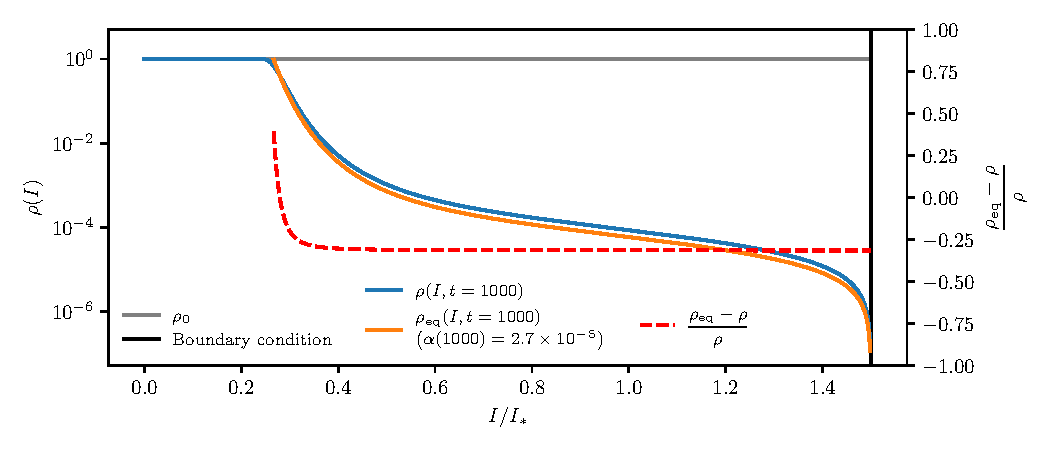
\includegraphics[width=\textwidth]{4_probing_the_diffusive_behavior/figs/final/new_stationary_distribution_s.pdf}
    \caption{Initial uniform distribution for the simulation shown in Fig.~\ref{fig:1} after numerical integration at $t=1000 \, [\text{a. u.}]$, compared to the estimate of $\rho_\mathrm{eq}$ from Eq.~\eqref{eq:equilibrium_stationary_distribution}, with $\alpha(t)$ computed with Eq.~\eqref{eq:alpha_with_time}. (Simulations parameters: $(I_\ast = 1.0\,[\sigma^2],\, \kappa = 0.33)$).}
    \label{fig:3}
\end{figure*}

%%%%%%%%%%%%%%%%%%%%%%%%%%%%%%%%%%%%%%%%%%%%%%%%%%%%%%%%%%%%%%%%%%%%%%%%%%%%%%%%

\section{Reconstruction of the diffusion coefficient of a FP process}
\label{sec:moving_the_absorbing_barrier}

%%%%%%%%%%%%%%%%%%%%%%%%%%%%%%%%%%%%%%%%%%%%%%%%%%%%%%%%%%%%%%%%%%%%%%%%%%%%%%%%

We now consider the problem of modelling the variation of the outgoing current after a change of the position $I_\mathrm{a}$ of the absorbing boundary condition, under the hypothesis that the movement is fast enough to be considered instantaneous, and the movement is performed over a short distance while the system is in the semistationary regime described in the previous section. The ultimate goal consists in defining a method to examine the information about the shape of the diffusion coefficient $D(I)$ contained in the outgoing current measured after the instantaneous movement of the boundary condition. This, in view of reconstructing the characteristics of the FP process under analysis, which corresponds to evaluating the values of the two parameters $I_\ast$ and $\kappa$ defining $D(I)$.

We define two types of outgoing current, namely \textsl{global current}, i.e.\ the outgoing current observed from a slow core erosion process while keeping the absorbing boundary condition fixed, and \textsl{recovery current}, i.e.\ the current observed after the absorbing boundary condition is instantaneously moved, and the system relaxes to a new semi-stationary regime.

We start by modelling the shape of the recovery current for a stationary system with a fixed source, both for inward and outward movements of the absorbing boundary. Furthermore, we recall that this mimics what is done experimentally when trying to measure the diffusion equation by performing scans of the position of some collimators jaws~{\cite{MESS1994279,flilleriii:pac03-rpag004,stancari2011diffusion,stancari:ipac11-tupz033,Stancari:1637929,PhysRevSTAB.16.021003,PhysRevAccelBeams.23.044802}}. Afterwards, we try to adapt the models to a system in semi-stationary regime, characterised by a source evolving with time.

%%%%%%%%%%%%%%%%%%%%%%%%%%%%%%%%%%%%%%%%%%%%%%%%%%%%%%%%%%%%%%%%%%%%%%%%%%%%%%%%

\subsection{Moving the absorbing boundary condition inwards}

%%%%%%%%%%%%%%%%%%%%%%%%%%%%%%%%%%%%%%%%%%%%%%%%%%%%%%%%%%%%%%%%%%%%%%%%%%%%%%%%

Let us consider a system in equilibrium with a constant  source $\rho(I_0, t)=1$, and an absorbing boundary condition $\rho(I_\mathrm{a}, t)=0$, and assume that the boundary condition is instantaneously moved inward to $\rho(I'_\mathrm{a}, t)=0$, with $I_0 < I'_\mathrm{a} < I_\mathrm{a}$. After this change, the equilibrium distribution varies and the new equilibrium distribution is given by
\begin{equation}
    \rho'_\text{eq}(I) = \beta \int_I^{I'_\mathrm{a}} \frac{1}{D(x)}\,\mathrm{d}x\,,
\end{equation}
where $\beta$ is a constant such that $\rho'_\text{eq}(I_0)=1$, and compared with the constant $\alpha$ of Eq.~\eqref{eq:equilibrium_stationary_distribution}, we have $\alpha < \beta$. The graphs of $\rho_\mathrm{eq}$ and $\rho'_\mathrm{eq}$ are shown in Fig.~\ref{fig:4} (top).

To apply the analytical formulae presented in the previous section, we need to compute the difference distribution $\rho^\ast(I)$. Assuming that the original system starts from the equilibrium distribution in Eq.~\eqref{eq:equilibrium_stationary_distribution}, we obtain 
\begin{align}
    \rho^\ast(I) = \rho_\text{eq}(I) - \rho'_\text{eq}(I) 
    &= \alpha \int_I^{I_\mathrm{a}} \frac{1}{D(x)}\,\mathrm{d}x - \beta \int_I^{I'_\mathrm{a}} \frac{1}{D(x)}\,\mathrm{d}x \notag \\
    &= \alpha \left( 
          \int_{I}^{I'_\mathrm{a}} \frac{1}{D(x)}\,\mathrm{d}x 
        + \int_{I'_\mathrm{a}}^{I_\mathrm{a}} \frac{1}{D(x)}\,\mathrm{d}x \right) - \beta \int_I^{I'_\mathrm{a}} \frac{1}{D(x)}\,\mathrm{d}x \notag \\
    &=  \alpha \int_{I'_\mathrm{a}}^{I_\mathrm{a}} \frac{1}{D(x)}\,\mathrm{d}x \, - (\beta - \alpha) \int_{I}^{I'_\mathrm{a}} \frac{1}{D(x)}\,\mathrm{d}x \notag \\
    &=  \rho^\ast_\text{app} - (\beta - \alpha) \int_{I}^{I'_\mathrm{a}} \frac{1}{D(x)}\,\mathrm{d}x \, .
    \label{eq:inward_difference}
\end{align}

The shape of $\rho^\ast(I)$ is shown in Fig.~\ref{fig:4} (bottom). This function, restricted to the interval $I \in [I_0, I'_\mathrm{a}]$, is increasing monotonously, with maximum in $I'_\mathrm{a}$. Given the Nekhoroshev-like form of the diffusion coefficient, the decrease to zero when $I \to I_0$ is exponentially fast, while in the region close to $I'_\mathrm{a}$, the function remains almost constant to the value $\rho^\ast_\text{app}$ that can be used as the lowest order approximation of $\rho^\ast(I)$.

\begin{figure*}[htp]
    \centering
    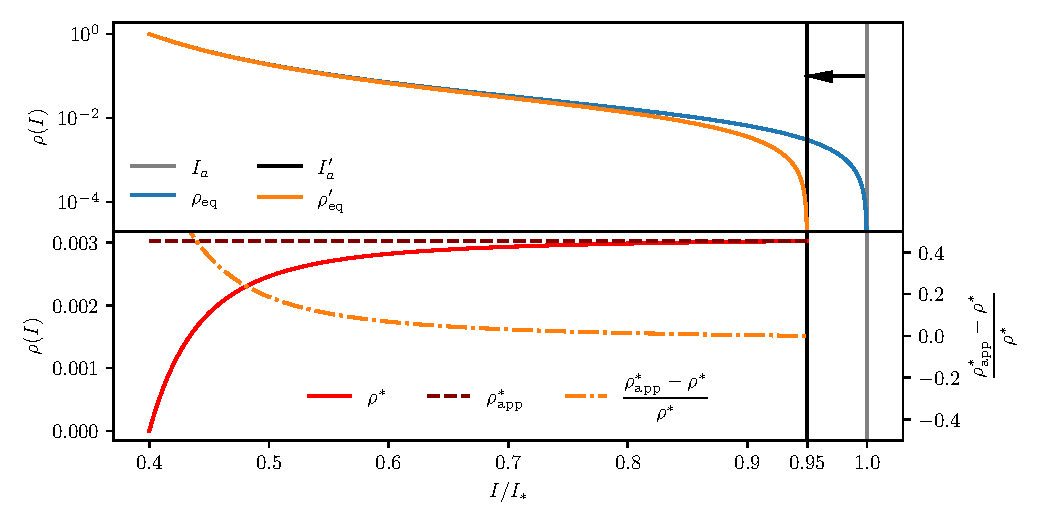
\includegraphics[width=\textwidth]{4_probing_the_diffusive_behavior/figs/final/difference_backwards_s.pdf}
    \caption{Top: Equilibrium distribution for $I_\mathrm{a}/I_\ast = 1.0$ compared with the  equilibrium distribution for $I'_\mathrm{a}/I_\ast = 0.95$. Bottom: Difference between the two equilibrium distributions. (Simulations parameters: $I_\ast = 1.0\,[\sigma^2],\, \kappa = 0.33,\, I_0/I_\ast = 0.4$).}
    \label{fig:4}
\end{figure*}

In Fig.~\ref{fig:5}, we compare the simulated current with its analytical estimate, obtained by computing the convolution with the distribution $\rho^\ast(I)$ of Eq.~\eqref{eq:inward_difference}, which are in very good agreement {(i.e.\ with a difference not greater than $10\%$)}. In the same figure, the analytical approximation based on the convolution with $\rho^\ast_\text{app}$ is shown, and even in this case the agreement is very good {(i.e.\ with a difference not greater than $10\%$)}.

\begin{figure*}[htp]
    \centering
    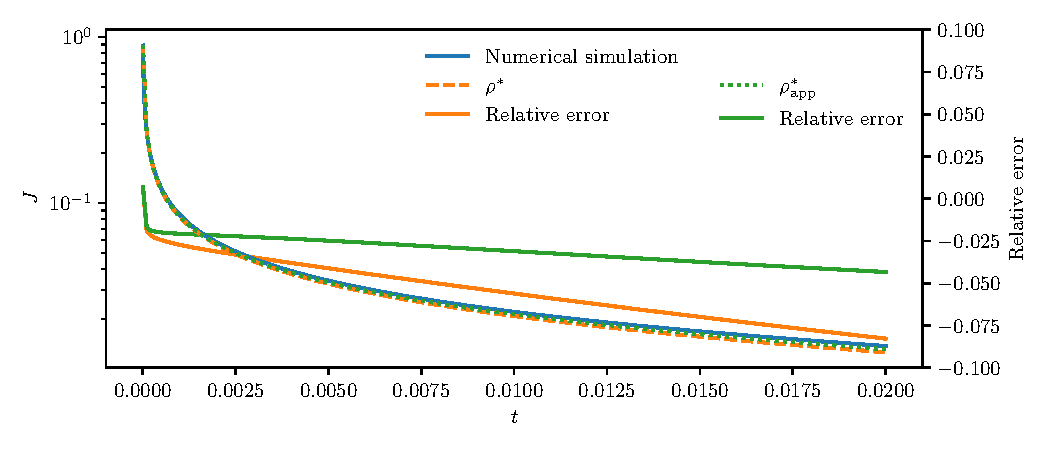
\includegraphics[width=\textwidth]{4_probing_the_diffusive_behavior/figs/final/current_backwards.pdf}
    \caption{Comparison between the current generated by the inward displacement of the absorbing boundary condition shown in Fig.~\ref{fig:4}, its analytical estimate based on $\rho^\ast(I)$, and the analytical estimate based on $\rho^\ast_\text{app}$.}
    \label{fig:5}
\end{figure*}

%%%%%%%%%%%%%%%%%%%%%%%%%%%%%%%%%%%%%%%%%%%%%%%%%%%%%%%%%%%%%%%%%%%%%%%%%%%%%%%%

\subsection{Moving the absorbing boundary condition outwards}

%%%%%%%%%%%%%%%%%%%%%%%%%%%%%%%%%%%%%%%%%%%%%%%%%%%%%%%%%%%%%%%%%%%%%%%%%%%%%%%%

Let us now consider a system in equilibrium with a constant source $\rho(I_0, t)=1$, and an absorbing boundary condition $\rho(I_\mathrm{a}, t)=0$, and assume that this boundary condition is instantaneously moved outward to $\rho(I''_\mathrm{a}, t)=0$, with $I_0 < I_\mathrm{a} < I''_\mathrm{a}$. The new equilibrium distribution is given by
\begin{equation}
    \rho''_\text{eq}(I) = \gamma \int_I^{I''_\mathrm{a}} \frac{1}{D(x)}\,\mathrm{d}x\,,
\end{equation}
where $\gamma$ is a constant such that $\rho''_\text{eq}(I_0)=1$, and compared with the constant $\alpha$ from Eq.~\eqref{eq:equilibrium_stationary_distribution}, we have $\gamma < \alpha$. The graphs of $\rho_\text{eq}(I)$ and $\rho''_\text{eq}(I)$ are shown in Fig.~\ref{fig:6} (top). 

To properly define the difference distribution in the new interval $[I_0, I''_\mathrm{a}]$, we need to extend the definition of the equilibrium distribution $\rho_\text{eq}(I)$, namely
\begin{equation}
    \rho_\text{eq}(I) = 
    \left\{\begin{array}{lr}
        \alpha \displaystyle{\int_I^{I_\mathrm{a}} \frac{1}{D(x)}\,\mathrm{d}x} \qquad & \text{if } \, I \leq I_\mathrm{a} \\
        \\
        0 \qquad & \text{if } \, I > I_\mathrm{a}\,,
    \end{array}\right.\,,
\end{equation}
which leads to the following expression for the difference distribution  
\begin{equation}
    \rho^\ast(I) = 
    \left\{\begin{array}{lr}
        - \gamma \displaystyle{\int_{I_\mathrm{a}}^{I''_\mathrm{a}} \frac{1}{D(x)}\,\mathrm{d}x + (\alpha - \gamma) \int_{I}^{I_\mathrm{a}} \frac{1}{D(x)}\,\mathrm{d}x}\ \quad &\text{if} \, I \leq I_\mathrm{a}\\
        \\
        - \gamma \displaystyle{\int_{I}^{I''_\mathrm{a}} \frac{1}{D(x)}\,\mathrm{d}x} \quad &\text{if} \, I > I_\mathrm{a}\,,
    \end{array}\right. 
    \label{eq:outward_difference}
\end{equation}
which is a negative distribution, with a minimum at $I_\mathrm{a}$ and with $\rho^\ast(I_0) = \rho^\ast(I''_\mathrm{a}) = 0$.

A plot of $\rho^\ast(I)$ is shown in Fig.~\ref{fig:6} (bottom), and we note that this distribution leads to a negative outgoing current that needs to be combined with the stationary current of the equilibrium process to obtain the actual outgoing current.

While in the interval $[I_0, I_\mathrm{a}]$ a constant approximated distribution function can be a reasonable assumption, in the interval $[I_\mathrm{a}, I''_\mathrm{a}]$ a different approximation is needed. Under the assumption that the outward step $I''_\mathrm{a} - I_\mathrm{a}$ is small, a linear approximation from $\rho^\ast(I_\mathrm{a})$ to $\rho^\ast(I''_\mathrm{a})$ can be considered, namely
\begin{equation}
    \rho^\ast_\text{app}(I) = 
    \left\{\begin{array}{lr}
        - \gamma \displaystyle{\int_{I_\mathrm{a}}^{I''_\mathrm{a}} \frac{1}{D(x)}\,\mathrm{d}x} \quad &\text{  if } \, I \leq I_\mathrm{a}\\
        \\
        - \gamma \displaystyle{\left(\frac{I''_\mathrm{a} - I}{I''_\mathrm{a} - I_\mathrm{a}} \right)} \displaystyle{\int_{I_\mathrm{a}}^{I''_\mathrm{a}} \frac{1}{D(x)}\,\mathrm{d}x} \quad &\text{  if } \, I > I_\mathrm{a} \,.
    \end{array}\right. 
    \label{eq:outward_difference_approx}
\end{equation} 

\begin{figure*}[htp]
    \centering
    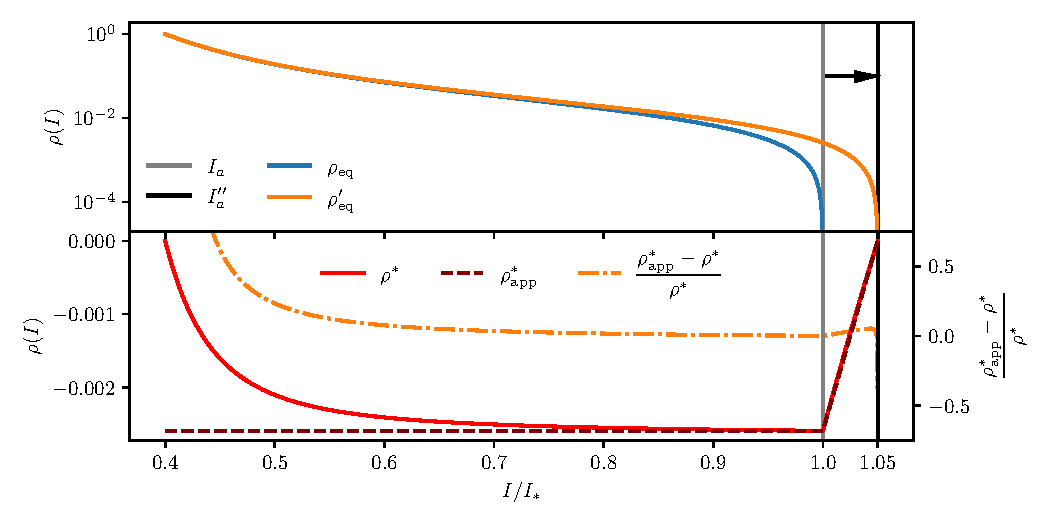
\includegraphics[width=\textwidth]{4_probing_the_diffusive_behavior/figs/final/difference_outwards_s.pdf}
    \caption{Top: Equilibrium distribution for $I_\mathrm{a}/I_\ast = 1.0$ compared with the equilibrium distribution for $I''_\mathrm{a}/I_\ast = 1.05$. Bottom: Difference between the two distributions. (Simulations parameters: $I_\ast = 1.0\,[\sigma^2],\, \kappa = 0.33,\, I_0/I_\ast = 0.4$).}
    \label{fig:6}
\end{figure*}

In Fig.~\ref{fig:7}, we compare the simulated current with its analytical estimate, obtained by computing the convolution with the distribution $\rho^\ast(I)$ of Eq.~\eqref{eq:outward_difference}, which is in good agreement {(i.e.\ with a difference not greater than $10-15\%$)}. In the same figure, the analytical approximation based on the convolution with $\rho^\ast_\text{app}$ is shown, and even in this case the agreement is excellent {(i.e.\ with a difference not greater than $5\%$)}.

\begin{figure*}[htp]
    \centering
    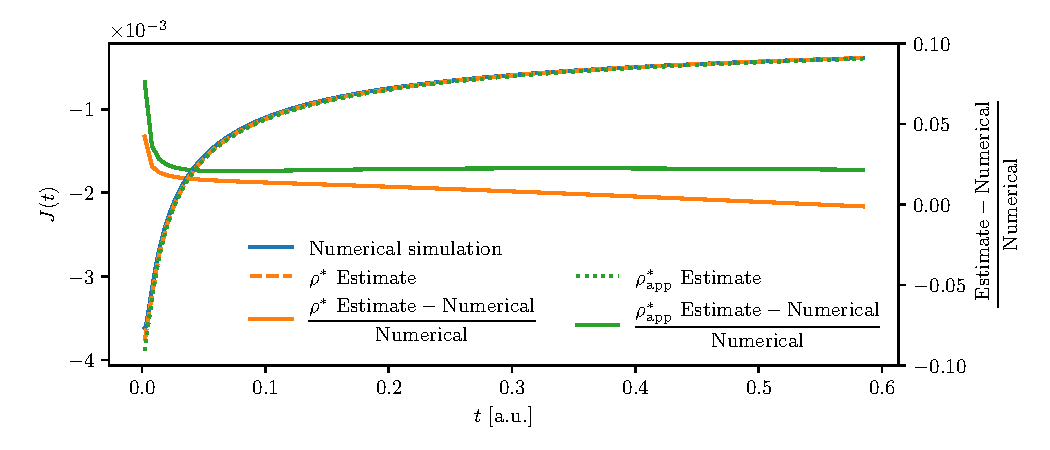
\includegraphics[width=\textwidth]{4_probing_the_diffusive_behavior/figs/final/current_outwards.pdf}
    \caption{Comparison between the current generated by the outward displacement of the absorbing boundary condition shown in Fig.~\ref{fig:6}, its analytical estimate based on $\rho^\ast(I)$, and the analytical estimate based on the approximation $\rho^\ast_\text{app}$.}
    \label{fig:7}
\end{figure*}

%%%%%%%%%%%%%%%%%%%%%%%%%%%%%%%%%%%%%%%%%%%%%%%%%%%%%%%%%%%%%%%%%%%%%%%%%%%%%%%%

\subsection{Moving the absorbing boundary condition in a semi-stationary system}
\label{subsec:Moving_the_boundary_in_a_semi_stationary_system}

%%%%%%%%%%%%%%%%%%%%%%%%%%%%%%%%%%%%%%%%%%%%%%%%%%%%%%%%%%%%%%%%%%%%%%%%%%%%%%%%

In Section~\ref{subsec:semi_stationary_regime_for_a_real_system} we have seen how it is possible to describe a diffusive process, after a transient time, as a semistationary process in which a stable core is slowly eroded over an exponentially long time, with an approximated timescale given by Eq.~\eqref{eq:peak_current_time}. If the position of the absorbing boundary condition is changed when the system is in this semi-stationary state, and the new position is close to the original one, so that it is characterised by a timescale of the same order of magnitude, the stationary part of the system, i.e.\ the relaxed part outside the stable-core, will relax to a new configuration in a time that is short compared to the timescale of the stable-core erosion.

Being the timescale of the recovery-current process orders of magnitude shorter than the evolution of the global current, the variation of the shape of the core is so slow that it can be neglected. Therefore, we can treat this situation as a source at a fixed position with a slow-varying intensity $\alpha(t)$. 

%%%%%%%%%%%%%%%%%%%%%%%%%%%%%%%%%%%%%%%%%%%%%%%%%%%%%%%%%%%%%%%%%%%%%%%%%%%%%%%%

\subsubsection{Normalizing a recovery current}

%%%%%%%%%%%%%%%%%%%%%%%%%%%%%%%%%%%%%%%%%%%%%%%%%%%%%%%%%%%%%%%%%%%%%%%%%%%%%%%%

Thanks to the previous assumptions, one can define a normalisation procedure to be applied to the recovery current to make it independent of the characteristics of the global current. We are interested in reducing the problem to the ideal case of a constant source at $I_0$ and a constant unitary outgoing current at the absorbing boundary condition $I_\mathrm{a}$, instead of a system with a slow-varying global current $\alpha(t)$. This approach is tested by simulating the same Nekhoroshev-like FP system twice: first, by keeping the absorbing boundary fixed; second, by executing some instantaneous changes of the absorbing boundary position. With this approach, we gather information on the value of the semi-stationary current $\alpha(t)$, thus enabling the transformation of the process with a moving boundary to a system with a fixed source.

We define the normalised recovery current as the current obtained in the measurement with the moving absorbing barrier divided by the current $\alpha(t)$, obtained in the measurement with fixed boundary. The normalised recovery current has a unitary value when the absorbing boundary condition is not changed and has normalised maximum and minimum, respectively, for the inward and outward movements of the absorbing boundary condition. The behaviour of the normalised recovery current can be related to the ideal stationary systems described above, for which analytical approximations are known.

In Fig.~\ref{fig:fixed-vs-moved-boundary}, an example of such a procedure is shown (centre) together with the evolution of the outgoing current (top) and the corresponding variation of the position of the boundary condition (bottom). It is worth mentioning that for every change of $I_\mathrm{a}$ the value of $\alpha(t)$ changes according to Eq.~\eqref{eq:alpha_with_time}, although for small variations of the absorbing boundary condition, a Taylor expansion can be applied.

\begin{figure*}[htp]
    \centering
    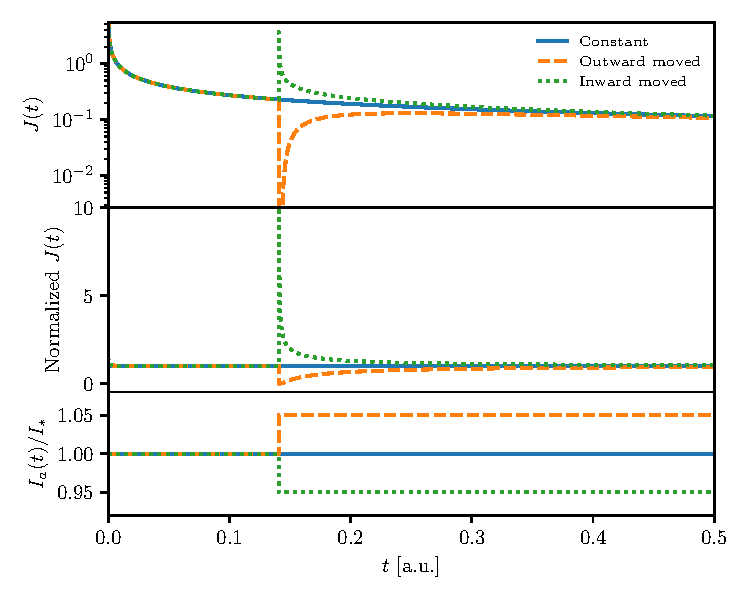
\includegraphics[width=\textwidth]{4_probing_the_diffusive_behavior/figs/final/global_vs_moving_current.pdf}
    \caption{Top: Evolution of the outgoing current for three diffusive processes with different boundary conditions. Middle: Evolution of the normalized outgoing current. Bottom: Changes to the absorbing boundary condition in the three scenarios. (Simulations parameters: $I_\ast = 1.0\,[\sigma^2], \, \kappa = 0.33$).}
    \label{fig:fixed-vs-moved-boundary}
\end{figure*}

%%%%%%%%%%%%%%%%%%%%%%%%%%%%%%%%%%%%%%%%%%%%%%%%%%%%%%%%%%%%%%%%%%%%%%%%%%%%%%%%

\subsubsection{Normalizing a recovery current without knowledge of the global current}

%%%%%%%%%%%%%%%%%%%%%%%%%%%%%%%%%%%%%%%%%%%%%%%%%%%%%%%%%%%%%%%%%%%%%%%%%%%%%%%%

Whenever it is not possible to repeat two complete measurements on the same process, i.e.\ one with and one without changes in the boundary condition position, the normalisation procedure defined previously needs to be adapted.

Ideally, the best strategy consists of waiting long enough after each change of the position of the absorbing boundary to reach an equilibrium and to accomplish the recovery process so that the outgoing current measured before the change of boundary position and after the long wait is a pure global current. This would approximately correspond to a complete relaxation of the difference distribution resulting from the boundary movement. Hence, in this way, the outgoing current can be used to reconstruct the shape of the global current and to perform the normalisation procedure.

However, some additional hurdles should be considered: Since we do not have prior knowledge of the value of $D(I)$, we do not know the timescales of the recovery currents or those of the core-eroding process. Furthermore, even though a good fraction of the recovery process is achieved very quickly, a complete recovery, corresponding to a complete relaxation of the difference distribution $\rho^\ast$, could take an exponentially long time, possibly beyond the computing capabilities. Hence, it might not be possible to perform such a long measurement in a particle accelerator. Therefore, it is necessary to define a protocol that enables quantitative criteria to establish whether or not an assumed recovery time is long enough to ensure a meaningful reconstruction of the behaviour of the FP process, possibly including an estimate of the uncertainty in the reconstruction of the global current.

A possible solution, compatible with these constraints, consists of the combination of three movements of the boundary condition, where, for each value of the action to be probed, an outward-inward-outward sequence of movements is performed. These three steps must be performed with a fixed movement size $\Delta I$ and with a fixed relaxation time $\Delta t$ between the movement of the boundary condition and the next. The optimal values for $\Delta I$ and $\Delta t$ are discussed in the next section. A visualisation of this protocol is provided in Fig.~\ref{fig:9} (bottom), where the change in boundary condition in three steps is highlighted and repeated three times, and the corresponding evolution of the outgoing current is given (top), calculated from numerical simulations. For comparison, the situation corresponding to the constant position of the boundary condition is also shown.

We remark that variants of the proposed three-step movement are indeed possible and that this proposal is also motivated by the wish not to introduce unnecessary complications. It is also important to stress that the assumption of performing small and equal movements of the position of the absorbing barrier for the three steps implies that also $\Delta t$ should be the same for the steps, since the relaxation time should be approximately the same for all steps. 

This three-step sequence of absorbing-barrier changes is performed at different values of the global current, and this basic sequence can be repeated by performing it at different action values. The resulting sequence of alternating recovery currents provides an approximation of the evolution of the global current with a sequence of upper- and lower-bound values at different times, which can be interpolated and used for the construction of a global current estimate. These limits provide a degree of uncertainty directly related to the chosen value $\Delta t$, as the longer $\Delta t$ is, the lower the degree of uncertainty in the reconstruction of the global current. A more detailed discussion of a possible quantitative definition of the optimal choice of the relaxation timescale $\Delta t$, together with the effects of using shorter relaxation times, is discussed in the next section.

To reconstruct the global current, an upper- and lower-bound estimate are derived by considering the last values of the inward and outward recovery currents, respectively. Two extra points are added to the upper- and lower-bound estimate, with the goal of covering the maximum time span for reconstructing the global current: The last measured global current value before the first boundary movement is added to both estimates; the last value of the last recovery current measured, which, being an outward recovery current, was already part of the lower-bound estimate, is also added to the upper-bound estimate. This explains why in Fig.~\ref{fig:protocol} (centre) the estimates coincide at the beginning and end of the interpolation interval. The two sets of upper-bound and lower-bound points are each interpolated with a univariate cubic spline and the average function of these two interpolating functions is taken as the estimate of the global current. 

We remark that the univariate cubic spline is taken with a number of knots so that the second derivative does not change sign. This ensures that the resulting global current estimate meets the expected features of the actual global current. In particular, it avoids local oscillations that might be generated by a simple interpolation of the upper-bound and lower-bound points. The result of this approach is shown in Fig.~\ref{fig:protocol} where a fraction of the data presented in Fig.~\ref{fig:9} is used to reconstruct the global current, and an excellent general agreement (i.e,\ with a difference not greater than $5\%$) with the actual global current is clearly visible.
%
\begin{figure*}[htp]
    \centering
    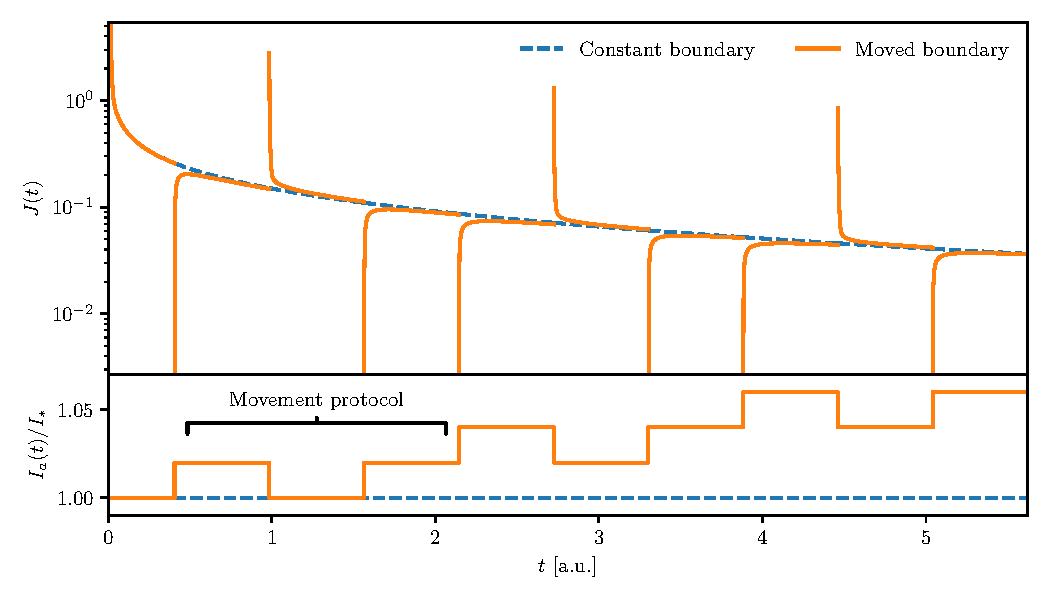
\includegraphics[width=\textwidth]{4_probing_the_diffusive_behavior/figs/final/the_protocol.pdf}
    \caption{Example of the proposed three-step protocol with a direct comparison between the condition with and without the variations in the position of the absorbing boundary condition. In this figure, the protocol is executed three times. The top plot shows the evolution of the outgoing current, while the bottom one shows the corresponding evolution of the position of the absorbing boundary condition. Note how the repetition of the three-step protocol moves progressively the absorbing boundary outwards. (Simulations parameters: $I_\ast = 1.0\,[\sigma^2],\,\kappa = 0.33$).}
    \label{fig:9}
\end{figure*}
%
\begin{figure*}[htp]
    \centering    
    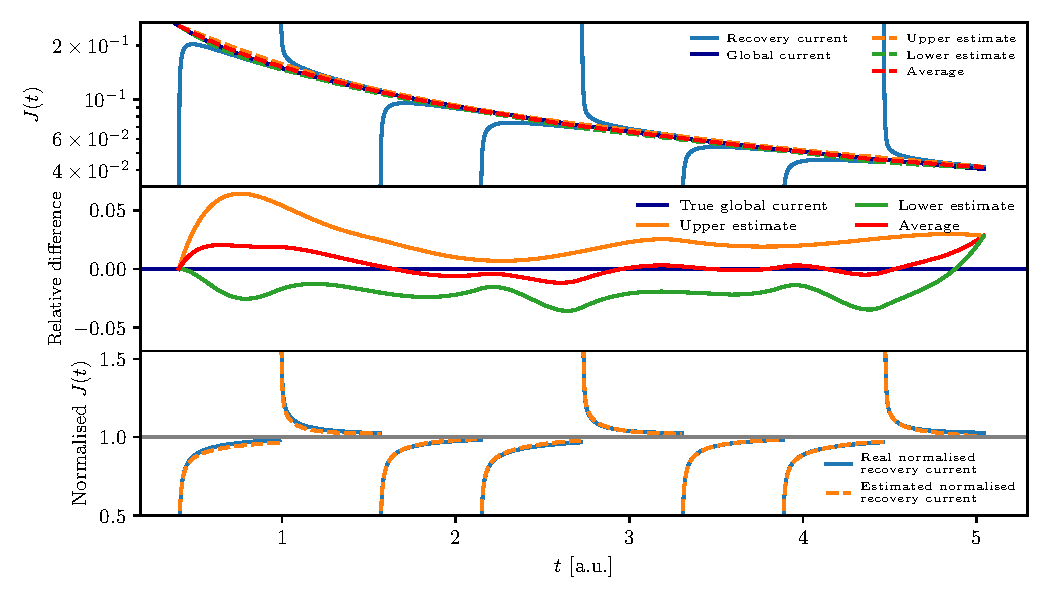
\includegraphics[width=\textwidth]{4_probing_the_diffusive_behavior/figs/final/the_interpolation.pdf}
    \caption{Example of the reconstruction process of the global current applied to a fraction of the data shown in Fig.~\ref{fig:9}. Top: Outgoing current from the process with constant boundary (dark blue) and with varying boundary conditions (light blue), along with the three components of the interpolation process. Middle: Relative difference, between the lower, average, or upper estimate of the global current and the true global current, of the interpolation procedure. Bottom: Comparison between the actual recovery current and the reconstructed one.}
    \label{fig:protocol}
\end{figure*}

%%%%%%%%%%%%%%%%%%%%%%%%%%%%%%%%%%%%%%%%%%%%%%%%%%%%%%%%%%%%%%%%%%%%%%%%%%%%%%%

\subsection{Reconstructing $D(I)$ from the normalized recovery currents}

%%%%%%%%%%%%%%%%%%%%%%%%%%%%%%%%%%%%%%%%%%%%%%%%%%%%%%%%%%%%%%%%%%%%%%%%%%%%%%%

After the proposed reconstruction protocol is performed, a series of normalised recovery currents, obtained for different positions of the boundary condition, are available. All these curves are then used to reconstruct the shape of $D(I)$ using a fit procedure.

Thanks to the normalisation procedure, every normalised recovery current can be considered as an individual and independent relaxation process, as in a system in equilibrium with a fixed source. Therefore, we can consider as expected current the convolution of the analytical current, presented in Eq.~\eqref{eq:thecurrent}, with one of our approximated difference distribution $\rho^\ast$, {according to Eq.~\eqref{eq:current_convolution}}. From a normalised recovery current obtained from an inward movement, we expect a relaxation curve characterised by an equivalent process with an initial distribution given by Eq.~\eqref{eq:inward_difference}, where the value of $\rho^\ast_\text{app}$ is calculated considering $\alpha=1$, due to the normalisation performed, the integral being calculated over the appropriate action interval. Likewise, for a recovery current from an outward movement, we expect a curve characterised by an equivalent process with an initial distribution given by Eq.~\eqref{eq:outward_difference_approx}, where we consider $\gamma=1$, due to the normalization performed, the integral being computed over the appropriate action interval. Assuming a Nekhoroshev-like form for $D(I)$, the goal is to determine the values of the two parameters $I_\ast$ and $\kappa$, which is obtained by a standard non-linear least squares algorithm applied to the currents obtained during the execution of the proposed protocol. {The strong non-linearity of the functions involved in the least-squares fit makes the reconstruction of $I_\ast$ and $\kappa$ a difficult task, and alternative approaches have been tried. A possibility consists in performing a coarse scan of the $(I_\ast, \kappa)$ parameter space to identify an initial guess of the model parameters, and then performing a finer scan around the initial guess. In this approach, the distance between the numerical value of the recovery current and the one obtained from the analytical model for a given pair of $(I_\ast, \kappa)$ values is evaluated, and the minimum provides either the initial estimate of the parameters or their optimal value. This strategy has been successfully applied to the analysis of beam data reported in~\cite{montanari:ipac22-mopost043}. Another aspect of the fit is the strong correlation between the model parameters, typically of the order of a Pearson product-moment coefficient of $0.9$, which is likely linked with the strongly non-linear function to be minimised. The impact of the strong correlation between the model parameters can be mitigated by the approach based on parameter scanning rather than looking for the minimum with standard routines to perform numerical optimisation.}

%%%%%%%%%%%%%%%%%%%%%%%%%%%%%%%%%%%%%%%%%%%%%%%%%%%%%%%%%%%%%%%%%%%%%%%%%%%%%%%%

\section{Numerical results}
\label{sec:numerical_results}

%%%%%%%%%%%%%%%%%%%%%%%%%%%%%%%%%%%%%%%%%%%%%%%%%%%%%%%%%%%%%%%%%%%%%%%%%%%%%%%%

To test the validity of the proposed procedure and obtain a complete overview of its performance and limitations in reconstruction of $D(I)$, several numerical simulations of diffusive processes with a Nekhoroshev-like diffusion coefficient have been performed using the protocol described in Section~\ref{sec:moving_the_absorbing_barrier}. Particular emphasis is placed on establishing the reliability of the proposed procedure as a function of the values of $\Delta I$ and $\Delta t$ used in the protocol of variation of the position of the boundary conditions.

%%%%%%%%%%%%%%%%%%%%%%%%%%%%%%%%%%%%%%%%%%%%%%%%%%%%%%%%%%%%%%%%%%%%%%%%%%%%%%%%

\subsection{Simulation parameters}

%%%%%%%%%%%%%%%%%%%%%%%%%%%%%%%%%%%%%%%%%%%%%%%%%%%%%%%%%%%%%%%%%%%%%%%%%%%%%%%%

As an initial condition, we consider the distribution in Eq~\eqref{eq:initial_distribution}, and note that all action variables are {dimensionless, and expressed either in units of sigma of the beam or in units of $I_\ast$}. We then consider a Nekhoroshev-like diffusive system characterised by the parameters obtained from the studies reported in Ref.~\cite{bazzani2020diffusion}, namely $I_\ast = 20.0\,[\sigma^2]$, $\kappa = 0.33$. Such a system, as can be seen from Figs.~\ref{fig:1} and~\ref{fig:3}, is compatible with the semi-stationary regime and hence with the application of the proposed procedure.

Different values of the starting position $I_\mathrm{a}/I_\ast$ of the absorbing boundary condition have been considered. Although most of our assumptions are valid for the $I_\mathrm{a}/I_\ast < 1$ regime, we also consider starting positions near $I_\ast$ and beyond $I_\ast$, i.e.\ in the saturation region of $D(I)$, to evaluate how robust the method is under non-ideal conditions.

For each configuration, after an initial time delay when a semi-stationary regime is reached, ten repetitions of the three-step protocol (outward-inward-outward), shown in Fig.~\ref{fig:9}, have been performed. Several values of $\Delta I$, i.e.\ the action change of the position of the boundary condition, have been used to assess the presence of an optimal value for the reconstruction procedure. We observe that at the end of a simulation, the position of the absorbing boundary condition has changed from $I_\mathrm{a}/I_\ast$ to $(I_\mathrm{a} + 10\Delta I) / I_\ast$. 

Several relaxation time values $\Delta t$ have been considered to evaluate reconstruction performance at different levels of equilibrium. We remark that an empirical relaxation time has been defined as the time for which a normalised recovery current is expected to recover the $99.9\%$ of the value of the original global current. Such an ideal time is computed using full knowledge of $D(I)$, using our analytical current estimate Eq.~\eqref{eq:thecurrent}, and considering an outward movement of the absorbing boundary condition of size $\Delta I$ from the initial position of the absorbing boundary. It is stressed that, in general, we should assume that such relaxation time is not known when reconstructing the value of the diffusion coefficient. It is also worth mentioning that a criterion based on a complete $100\%$ recovery of the global current cannot be used in practice, as this would require exponentially long simulation times, needed to reach the relaxation of the inner part of the distribution, with negligible differences with respect to the $99.9\%$ case. Different fractions of this ideal time have been used when performing our procedure, and we evaluate how times shorter than the ideal relaxation time impact the quality of our final fit, as the system is still in a non-equilibrium regime when the next absorbing boundary movement occurs.

When working with the data sets generated by the various numerical simulations, a post-processing step is performed on the normalised recovery currents before executing the final fit procedure for reconstructing $D(I)$. It consists of selecting a fraction of the data representing the normalised recovery currents, i.e.\ only the normalised recovery current data up to a given percentage of the full recovery. For example, if we decide to filter out normalised data beyond the $90\%$ recovery, it means that we discard values that are lower than $1.1$ for inward normalised recovery currents and values that are higher than $0.9$ for outward normalised recovery currents. We recall that, in the context of a normalised recovery current, a full recovery implies a value of $1.0$ as a normalised recovery current.

This post-processing step is shown in Fig.~\ref{fig:postprocessing}, where two different values of the fraction of the relaxation time between boundary movements are used in the numerical simulations. In both simulations, the boundary movement starts after an equal waiting time. In the left plot, the normalised recovery currents, reported in Fig.~\ref{fig:protocol}, are shown together with two different filtering levels. On the right, the same system is simulated using a shorter fraction of the relaxation time, and the recovery currents are shown together with the same filtering levels presented in the left plot. The much shorter time leads to only a partial recovery of the currents between boundary condition changes. For these sets of normalised recovery currents, the filtering levels displayed lead to almost no data reduction.
%
\begin{figure*}[htp]
    \centering 
    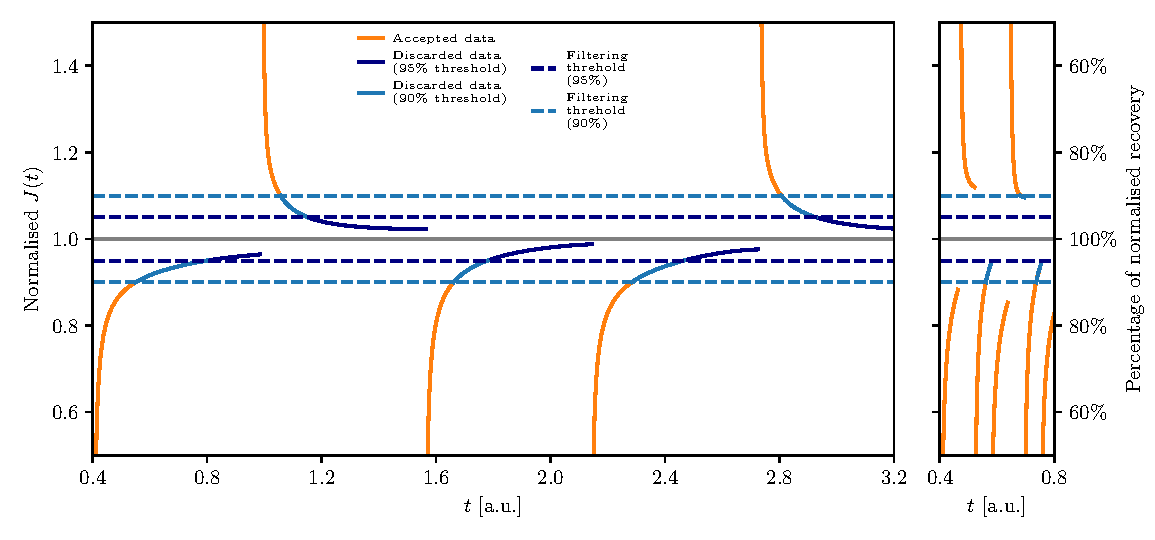
\includegraphics[width=\textwidth]{4_probing_the_diffusive_behavior/figs/final/the_discarded_data.pdf}
    \caption{Left: normalized recovery current, shown already in Fig.~\ref{fig:protocol}, together with two filtering levels. The boundary movements are performed after an initial evolution time $t=0.4 \, [\text{a. u.}]$, and the relaxation time $\Delta t$ between one boundary movement and the next one is equal to $\Delta t=0.58 \, [\text{a. u.}]$. Right: the same system is simulated with the same initial evolution time $t=0.4 \, [\text{a. u.}]$ and one order of magnitude shorter relaxation time $\Delta t=0.058 \, [\text{a. u.}]$, the resulting normalized recovery currents have not relaxed long enough to reach the $95\%$ filtering level. When the selected filtering level is not reached by the normalized recovery currents, the whole dataset is used for the fit reconstruction and no parts are discarded.}
    \label{fig:postprocessing}
\end{figure*}
%

By selecting different levels of data filtering, it is possible to evaluate how this choice affects the accuracy of the reconstruction of $D(I)$. It should be noted that our analytical approximation of Eq.~\eqref{eq:thecurrent} performs best when describing the evolution of a distribution near the absorbing boundary condition~\cite{montanari:ipac2021:tupab233}. Furthermore, the recovery current features an exponential-like decay that makes the analytical approximation less accurate over long timescales. For this reason, investigating the dependence of the reconstruction performance on the fraction of data selected is very relevant.

%%%%%%%%%%%%%%%%%%%%%%%%%%%%%%%%%%%%%%%%%%%%%%%%%%%%%%%%%%%%%%%%%%%%%%%%%%%%%%%%

\subsection{Analysis of the reconstruction performance}

%%%%%%%%%%%%%%%%%%%%%%%%%%%%%%%%%%%%%%%%%%%%%%%%%%%%%%%%%%%%%%%%%%%%%%%%%%%%%%%%

Numerical exploration of the FP process involves a scan of several simulation parameters, leading to a large hyperspace of possible configurations. For this reason, we focus on the most ideal configurations, i.e.\ those that provide the best reconstruction performance, and then show how the other parameters affect the reconstruction accuracy of $I_\ast$ and $\kappa$.

After each execution of the proposed three-step protocol described in Section~\ref{sec:moving_the_absorbing_barrier} and shown in Fig.~\ref{fig:9}, we end up with two outward and one inward recovery currents. In every configuration explored, we observe better reconstruction results when only the recovery currents from the outward step are considered. On the other hand, considering only the inward recovery currents or all currents simultaneously, poorer performance and numerical instabilities are observed. This is explained by the fact that when the position of the absorbing boundary is moved inward, we are cutting in a distribution that is not necessarily in the perfect equilibrium configuration defined in our approximations. On the other hand, when we move the boundary condition outward, we obtain a much more reliable observable of the distribution that populates the new available action interval, when evolving towards the new equilibrium state. It is possible to observe this behaviour in Fig.~\ref{fig:all_different_time}, where the relative error in the reconstruction of $\kappa$ and $I_\ast$ is shown for the three types of fit as a function of the fraction of the ideal relaxation time $\Delta t$ for two values of $I_\mathrm{a}/I_\ast$, representing the inner part of the stable-core region (left) and close to the regime change of $D(I)$ (right). In the inner region, even small fractions of the relaxation time provide a good reconstruction of the fit parameters {(i.e.\ with a difference not greater than $10-15\%$)}. Furthermore, the three types of analysis, based on outward-only, inward-only, and inward and outward recovery currents, provide results with comparable accuracy for longer fractions of the relaxation time.  
%
\begin{figure*}[htp]
    \centering
    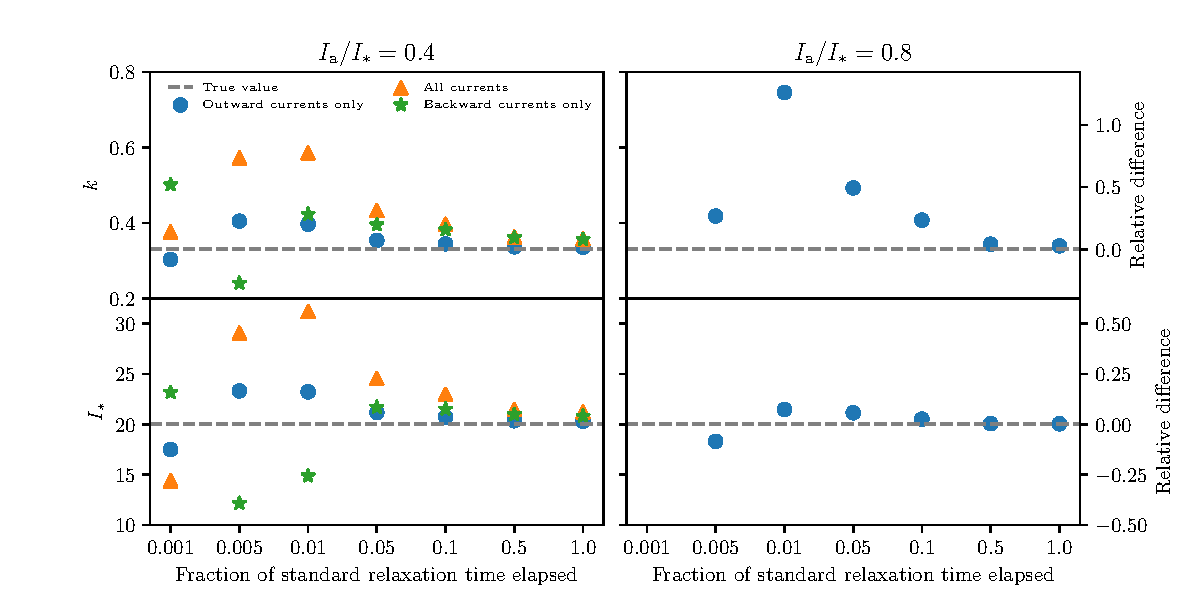
\includegraphics[width=\textwidth]{4_probing_the_diffusive_behavior/figs/final/better_plot.pdf}
    \caption{Fit results for $I_\ast$ and $\kappa$ as a function of the relaxation time $\Delta t$ for two values of $I_\mathrm{a}/I_\ast$, using different subsets of the numerical data. Left: for $I_\mathrm{a}/I_\ast=0.4$, a good reconstruction performance  {(i.e.\ with a difference not greater than $20\%$)} is observed even for short fractions of the ideal relaxation time. A rather similar performance is observed for the three types of analysis, the one based on the outward currents having the best performance. Right: for $I_\mathrm{a} / I_\ast=0.8$, only the cases corresponding to longer fractions of the relaxation time feature a good performance. Moreover, only the analysis based on the outward currents is displayed, as the other two features either failures or large errors in the fit. (Simulation parameters: initial $I_\mathrm{a}/I_\ast=0.4$, boundary step $\Delta I =0.1 \sigma^2$, 10 repetitions of the three-step procedure, data up to a maximum current recovery of $90\%$).}
    \label{fig:all_different_time}
\end{figure*}
%

However, in the transition region, only longer fractions of relaxation time provide a good reconstruction of the fit parameters  {(i.e.\ with a difference not greater than $20\%$)} and the only applicable type of analysis is that based on outward recovery currents. The other two analyses feature failures or larger errors in the fit, {which are generated by the behaviour of the inward recovery current}. On the basis of the observed behaviour, in the next plots, we will only display results from the reconstruction based on the outward recovery currents. {The reasons for the poor performance of the reconstruction of $I_\ast$ and $\kappa$ when inward recovery currents are considered are at least twofold. The first reason stems from the fact that by cutting the distribution with the inward movement of the boundary condition, the system enters a non-equilibrium regime, in which the recovery current features sizeable variations. If enough time is elapsed, the system reaches a new equilibrium, and the recovery current is much more reliable for the reconstruction of $I_\ast$ and $\kappa$, as observed in Fig.~\ref{fig:all_different_time}. The second reason is of purely numerical origin, but somewhat linked to the first one, as when an inward step is performed, the equilibrium distribution is cut and the sharp edge needs to be smoothed by applying a logistic function to the cut distribution (see the discussion in Appendix~\ref{app_sec:numerical_integration_with_crank_nicolson}). This has potentially harmful effects on the generated recovery current, which is subsequently used to reconstruct the model parameters. Note that the first argument is even more applicable to the case of data from beam experiments, as observed from the data analyses carried out recently and discussed in Ref.~\cite{montanari:ipac22-mopost043}.}

In Fig.~\ref{fig:different_position}, the reconstruction error for the two fit parameters is shown as a function of the starting position of the absorbing boundary $I_\mathrm{a}/I_\ast$. 
%
\begin{figure*}[htp]
    \centering
    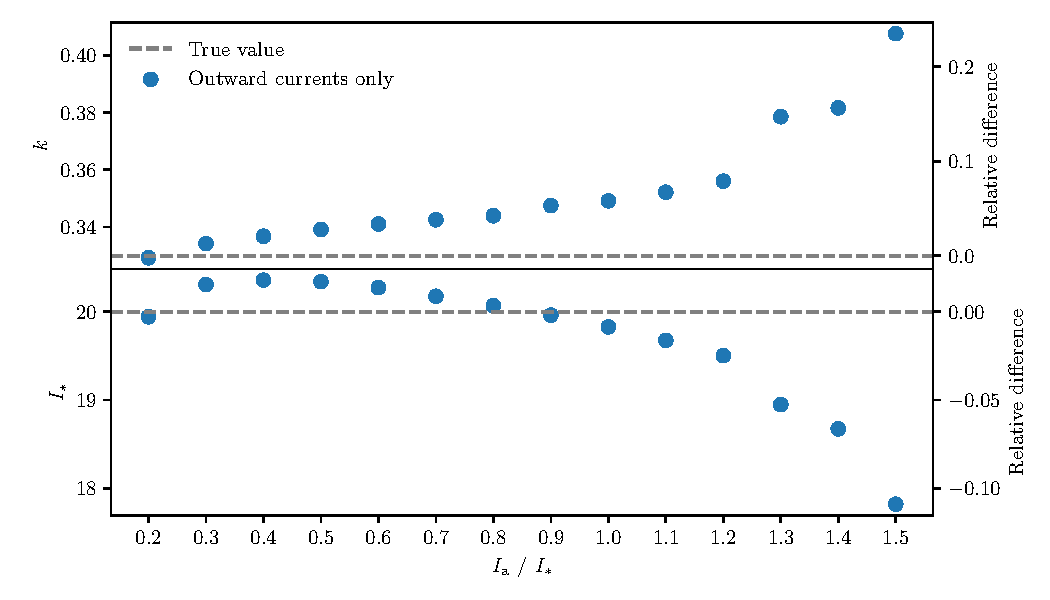
\includegraphics[width=\textwidth]{4_probing_the_diffusive_behavior/figs/final/different_position.pdf}
    \caption{Fit results for $I_\ast$ and $\kappa$ as a function of the initial value of $I_\mathrm{a}/I_\ast$. The reconstruction performance is excellent for $I_\mathrm{a}/I_\ast \leq 1$, while for larger values the relative error increases. (Simulation parameters: boundary step $\Delta I=0.1 \sigma^2$, relaxation time $\Delta t=0.5$, 10 repetitions of the three-step procedure, data up to a maximum current recovery of $90\%$).}
    \label{fig:different_position}
\end{figure*}
%
The performance is excellent for $I_\mathrm{a}/I_\ast \leq 1$ {(i.e.\ with a difference not greater than $5\%$)}, while outside this region the reconstruction error increases. This behaviour is to be expected, as a recovery current carries mainly local information about $D(I)$. Therefore, if only the region $I_\mathrm{a}/I_\ast > 1$ is sampled, the information about $D(I)$ reflects only its quasi-linear regime (see Fig.~\ref{fig:1}). Such incomplete information inevitably affects the performance of the final fit, as it prevents an accurate reconstruction of the strongly non-linear part of the diffusion coefficient. This result also suggests that after the fit parameters have been determined, one can verify whether the action interval explored was suitable for an accurate reconstruction of the functional form of the diffusion coefficient.

The plots in Fig.~\ref{fig:different_position} provide some insight into the dependence of the reconstruction performance as a function of a single parameter while the others are kept fixed. However, in the following figures, the relative error of the reconstruction procedure is shown as a function of two parameters. The colour code represents the relative difference between the reconstructed values (from the proposed protocol) and the true values (used in numerical simulations of the FP processes) of $I_\ast$ and $\kappa$ that describe $D(I)$. The scale is limited to a relative difference of $20\%$, which is assumed as a threshold to identify poor performance. Note that white cells represent cases in which the reconstruction procedure failed.

Figure~\ref{fig:different_cut} shows the relative error as a function of the cut in recovery current performed during post-processing and $I_\mathrm{a}/I_\ast$. The performance of the reconstruction approach improves when the recovery currents are cut. This depends on the fact that our approach is local, i.e.\ accurate to describe the system's behaviour close to the boundary condition. The longer the recovery time, the less local the information gathered from the current. For this reason, the plots on reconstruction performance are based on recovery currents cut at $90\%$. 

\begin{figure*}[htp]
    \centering
    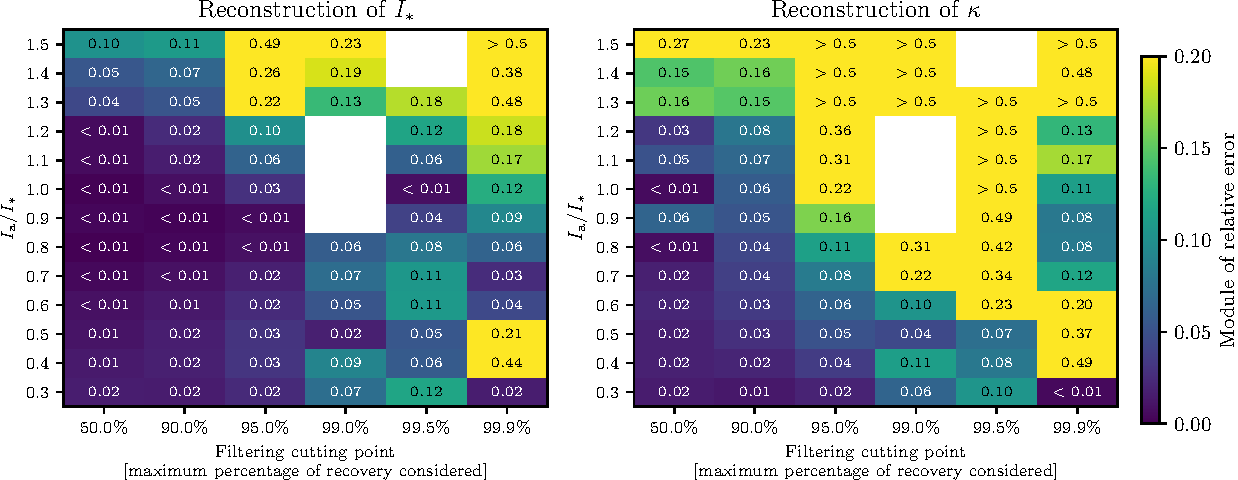
\includegraphics[width=\textwidth]{4_probing_the_diffusive_behavior/figs/final/MULTI_different_filter.pdf}
    \caption{2D view of the reconstruction performance as a function of the cut in the recovery current, as applied in Fig.~\ref{fig:postprocessing}, and of the initial value of $I_\mathrm{a}/I_\ast$. It is clearly seen how certain values of the cut provide a consistent increase in reconstruction performance. White regions indicate a failure in convergence in the final fit procedure. (Simulation parameters: relaxation time $\Delta t=1$, boundary step $\Delta I=0.1 \sigma^2$, 10 repetitions of the three-step, data up to a maximum current recovery of $90\%$).}
    \label{fig:different_cut}
\end{figure*}

Regarding the reconstruction performance as a function of the relaxation time $\Delta t$, Fig.~\ref{fig:different_time} shows the behaviour, including the dependence on $I_\mathrm{a}/I_\ast$. In this case, the longer the relaxation time, the better the reconstruction performance. In particular, longer relaxation times allow for a better reconstruction even for large values of $I_\mathrm{a}/I_\ast$. It should be noted that, in the case of short relaxation times, good overall performance can only be achieved by working at $I/I_\ast \ll 1$.
%
\begin{figure*}[htp]
    \centering
    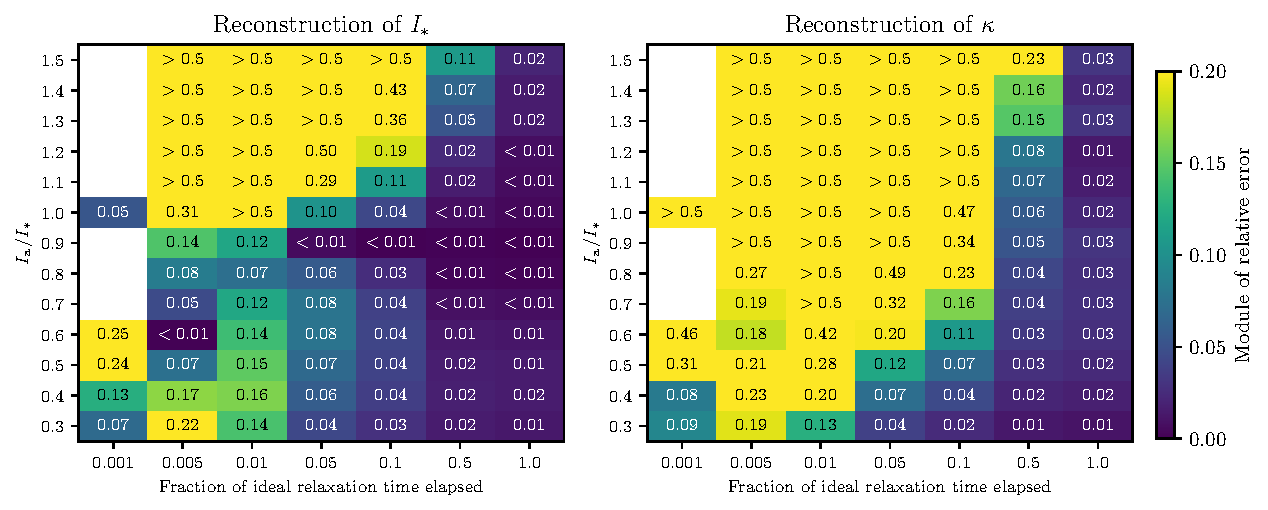
\includegraphics[width=\textwidth]{4_probing_the_diffusive_behavior/figs/final/MULTI_different_time.pdf}
    \caption{2D view of the reconstruction performance as a function of the relaxation time $\Delta t$ and the initial value of $I_\mathrm{a}/I_\ast$. It is clearly seen how the reconstruction performance improves for longer relaxation times. However, the method proves to be rather robust for fractions of ideal time up to $5\%$ provided $I_\mathrm{a}/I_\ast < 0.6$. White regions indicate a failure in convergence in the final fit procedure. (Simulation parameters: boundary step $\Delta I=0.1 \sigma^2$, 10 repetitions of the three-step procedure, data up to a maximum current recovery of $90\%$, if smaller values of $\Delta t$ lead to a normalized recovery below $90\%$, all the normalized recovery current data are used for the reconstruction).}
    \label{fig:different_time}
\end{figure*}
%
Combining the results of the last two analyses, one concludes that the best approach to an accurate determination of $I_\ast$ and $\kappa$ consists of increasing the relaxation time between successive changes in the position of the boundary condition and cutting the data from the recovery currents. 

Figure~\ref{fig:different_nsamples} shows the 2D plot of reconstruction performance as a function of the number of repetitions of the three-step procedure and $I_\mathrm{a}/I_\ast$. It can be seen with the higher number of repetitions how the performance improves. This is naturally linked to the fact that repeating the three-step procedure implies sampling a larger extent of the phase space, thus probing more accurately the behaviour of the diffusion coefficient as a function of the action. It is also clearly visible that from six repetitions of the three-step procedure, a good reconstruction is obtained for $I_\mathrm{a}/I_\ast < 1$.

\begin{figure*}[htp]
    \centering
    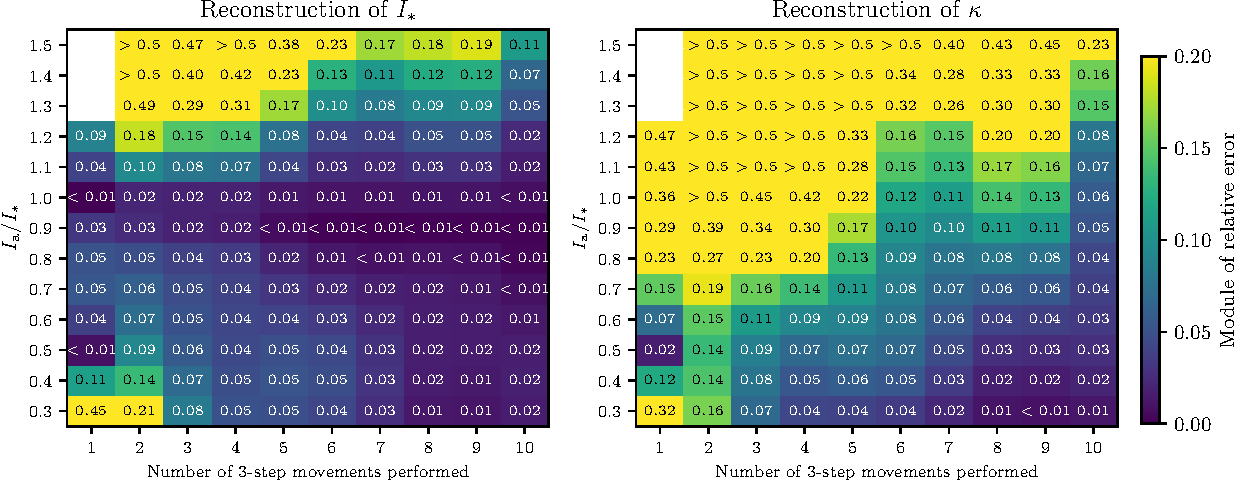
\includegraphics[width=\textwidth]{4_probing_the_diffusive_behavior/figs/final/MULTI_different_samples.pdf}
    \caption{2D view of the reconstruction performance as a function of the number of three-step movements and of $I_\mathrm{a}/I_\ast$ starting positions. It is clearly seen how the performance increases with the number of three-step movements, as larger regions of phase space are explored (as in Fig.~\ref{fig:9}). White regions indicate a failure in convergence in the final fit procedure. (Simulation parameters: relaxation time $\Delta t=0.5 \, [\text{a. u.}]$, boundary step $\Delta I=0.1 \sigma^2$, which is $\Delta I / I_\ast = 0.005$, data up to a maximum current recovery of $90\%$ is considered).}
    \label{fig:different_nsamples}
\end{figure*}

Finally, the impact of $\Delta I$ is shown in Fig.~\ref{fig:different_movement_module}, where the performance is represented as a function of $\Delta I$ and $I_\mathrm{a}/I_\ast$ is represented.  We see that performance is not strongly affected by the choice of $\Delta I$, i.e.\ relative error fluctuations are less than $10\%$ for differences of an order of magnitude in $\Delta I$. However, it is important to highlight two facts that could suggest a choice in the size of the change in position of the absorbing boundary condition: (1) the ideal relaxation time is directly proportional to the size of the absorbing boundary movement; (2) a too small $\Delta I$ could lead to a too local sampling in the action space, thus negatively affecting the final reconstruction of $D(I)$. 

\begin{figure*}[htp]
    \centering
    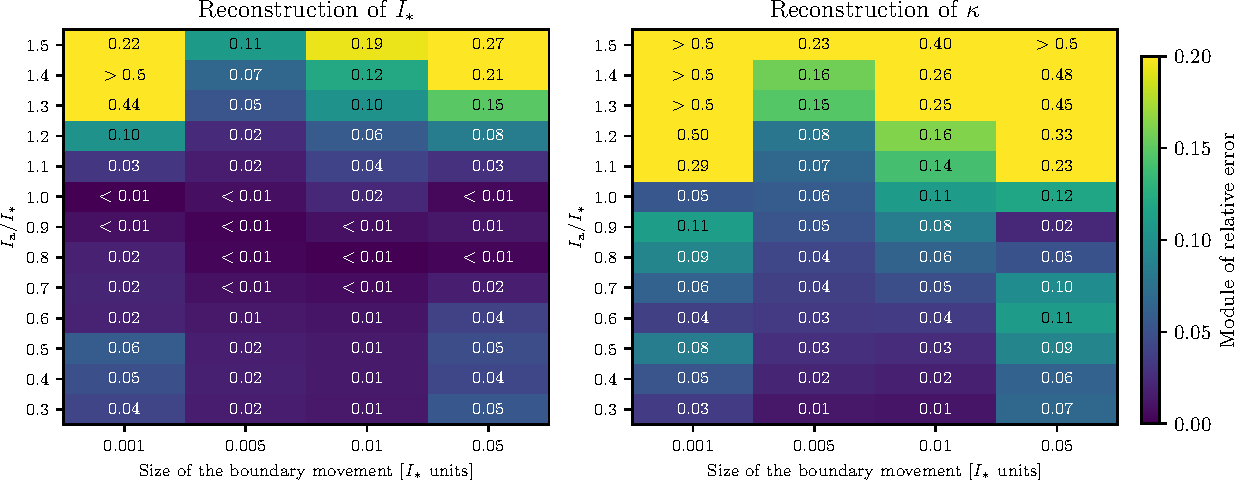
\includegraphics[width=\textwidth]{4_probing_the_diffusive_behavior/figs/final/MULTI_different_step_size.pdf}
    \caption{2D view of the reconstruction performance as a function of $\Delta I$ and $I_\mathrm{a}/I_\ast$. The  best performance is achieved for $\Delta I = 0.005 \sigma^2$, but the dependence on $\Delta I$ is very weak (Simulation parameters: relaxation time $\Delta t=0.5 \, [\text{a. u.}]$, 10 repetitions of the three-step procedure, data up to a maximum current recovery of $90\%$).}
    \label{fig:different_movement_module}
\end{figure*}

%%%%%%%%%%%%%%%%%%%%%%%%%%%%%%%%%%%%%%%%%%%%%%%%%%%%%%%%%%%%%%%%%%%%%%%%%%%%%%%%

\section{Final remarks}
\label{sec:conclusions}

%%%%%%%%%%%%%%%%%%%%%%%%%%%%%%%%%%%%%%%%%%%%%%%%%%%%%%%%%%%%%%%%%%%%%%%%%%%%%%%%

Beam-halo scans, performed with movable collimator jaws, have been used intensively for probing the diffusive behaviour of the beam halo in circular accelerators and seem to be a very useful tool for probing this special regime of beam dynamics in the absence of beam instrumentation capable of providing diagnostic tools to study beam-halo dynamics.

{The main result of this chapter} is the identification of an efficient protocol for testing the shape of {a diffusion coefficient consistent with the stability time estimate of the Nekhoroshev theorem}. The protocol has been scrutinised by means of detailed numerical simulations, {but} it is clear that eventually it should be tested with beam measurement data. Two aspects should be highlighted: although the framework presented in this article is one-dimensional, i.e.\ considering non-linear beam dynamics in one degree of freedom, we believe that it can be applied to cases representing systems with two degrees of freedom (as shown in Ref.~\cite{bazzani2020diffusion}). Furthermore, the proposed approach does not rely on previous knowledge of the beam distribution, which is a clear advantage for applications. 
 
The proposed protocol relies on the idea that it is possible to separate the measured outgoing current into a global current, i.e.\ the general outgoing current loss that is measured from the exponentially slow erosion of the stable core of the beam, and a recovery current, i.e.\ the current following a change of the position of the boundary condition, which corresponds to a non-equilibrium state. By performing an alternating three-step sequence of outward-inward-outward boundary-condition changes, which can easily be done by means of collimator scans, it is possible to reconstruct the global current of the erosion process and use that to normalise the recovery currents. Each normalised recovery current ultimately contains local information on the diffusion coefficient without the need of prior knowledge on the form of the initial distribution in action space and can be used for estimating its global shape.

The performance of this protocol has been tested by means of many numerical simulations of Fokker-Planck processes performed in various configurations to evaluate the reliability and limits of our approach. The protocol was shown to be capable of reconstructing with precision and good accuracy  {(i.e.\ with an error not greater than $10-15\%$)} the parameters of the diffusion coefficient when performed in a phase-space region where the diffusion coefficient has an exponential evolution, i.e.\ for $I/I_\ast < 1$, the relaxation time between changes in the boundary conditions is long enough so that the system reaches an equilibrium state and multiple amplitudes have been probed. For this last condition, the optimal number of amplitudes to be sampled is highly dependent on the detail of the diffusion process; however, from the simulations it appears that about six sequences of three-step absorbing boundary changes covering the $I / I_\ast < 1$ region is a good choice. 

The analysis also highlighted how a good reconstruction performance can be achieved by considering only the outgoing recovery currents in the final fitting reconstruction and by discarding part of the recovery current data beyond a certain level, as it is more prone to reconstruction errors and more difficult to characterise with our analytical formulas. It is worth stressing that the reconstruction performance proves to be good even if the optimal conditions are not fully met. Most importantly, the procedure provides useful information on possible shortcomings present in the data set under consideration, such as a high uncertainty band in the global current reconstruction, or a reconstructed value of $I_\ast$ that indicates that the probed phase-space region is outside the optimal interval $I / I_\ast < 1$. In these cases, the protocol should be re-applied in better conditions, e.g.\ by adjusting the range of actions probed to satisfy the condition $I / I_\ast < 1$.

Thanks to the positive and encouraging results of the analysis presented here, we are confident that the measurement protocol is a powerful tool for probing the non-linear diffusive behaviour in an accelerator like the LHC, although it should be stressed that it is of general applicability in any circular accelerator. Therefore, the logical next step is the proposal of a dedicated beam measurement, at the LHC or elsewhere, performed in the optimal conditions considered in this Chapter, which will complete the investigations presented in this Chapter. In the meantime, available data from collimator scans collected at the LHC (but not with the proposed protocol), have been analysed under the assumption of the proposed functional form for the diffusion coefficient. Very promising results have been obtained that support pursuing this line of research, and will be presented in the next Chapter.
\chapter{Diffusion measurements at the CERN LHC}\label{ch:diffusion_meas}
\noindent\textsf{The content of this chapter, with the due adaptations, has resulted in the proceedings by C.\ E.\ Montanari, A.\ Bazzani, M.\ Giovannozzi, A.\ A.\ Gorzawski, and S.\ Redaelli \textit{\citetitle{montanari:ipac22-mopost043}}, which were presented as a poster at IPAC'22 in June 2022~(Ref.~\cite{montanari:ipac22-mopost043}).}

\vspace{3em}

In Chapter~\ref{ch:probing}, we presented an optimal method to measure the diffusion coefficient of a beam halo, based on the characteristics of the outgoing current, given by a Fokker-Planck equation with a Nekhoroshev-like diffusion coefficient. In this chapter, we apply this method to the available LHC collimator scan data, which was gathered during Run~2, however, not using the optimized measurement protocol devised in the previous chapter.

As this measurement campaign was tailored to a different model of diffusion, the data was gathered with a different protocol, which inevitably does not meet all the optimal requirements highlighted in the previous chapter. This inevitably required an adjustment of the reconstruction procedure to account for the differences between the optimal and the actual measurement protocol.

The chapter is structured as follows. In Section~\ref{sec:4:collimation}, we present the LHC collimation system. In Section~\ref{sec:4:analysis}, we present the collimator scan data and the diffusion coefficient reconstruction, together with the necessary adjustments applied to the reconstruction procedure to account for the differences between the optimal and the actual measurement protocol. Finally, some conclusive remarks are given in Section~\ref{sec:4:remarks}.

\section{The LHC collimation system}\label{sec:4:collimation}

The LHC layout~\cite{Bruning:782076} can be summarized in a geometric scheme composed of eight straight insert regions (IR) and eight circular arc segments. A simple scheme of this layout is reported in Fig.~\ref{fig:lhc_layout}, left. Within this circular scheme, the main particle physics experiments are located in IR1, IR2, IR5 and IR8, namely, ATLAS~\cite{TheATLASCollaboration_2008}, ALICE~\cite{Alessandro:879894}, CMS~\cite{Chatrchyan:1129810}, and LHCb~\cite{Alves:1129809}. In these four IRs, the two beams intersect and interact in what is referred to as an Interaction Point (IP). The RF cavities for accelerating the beams are in IR4 and IR6 hosts the beam extraction system. Finally, IR3 and IR7 are dedicated, respectively, to the longitudinal and transverse collimation system.

\begin{figure}[hpt]
    \centering
    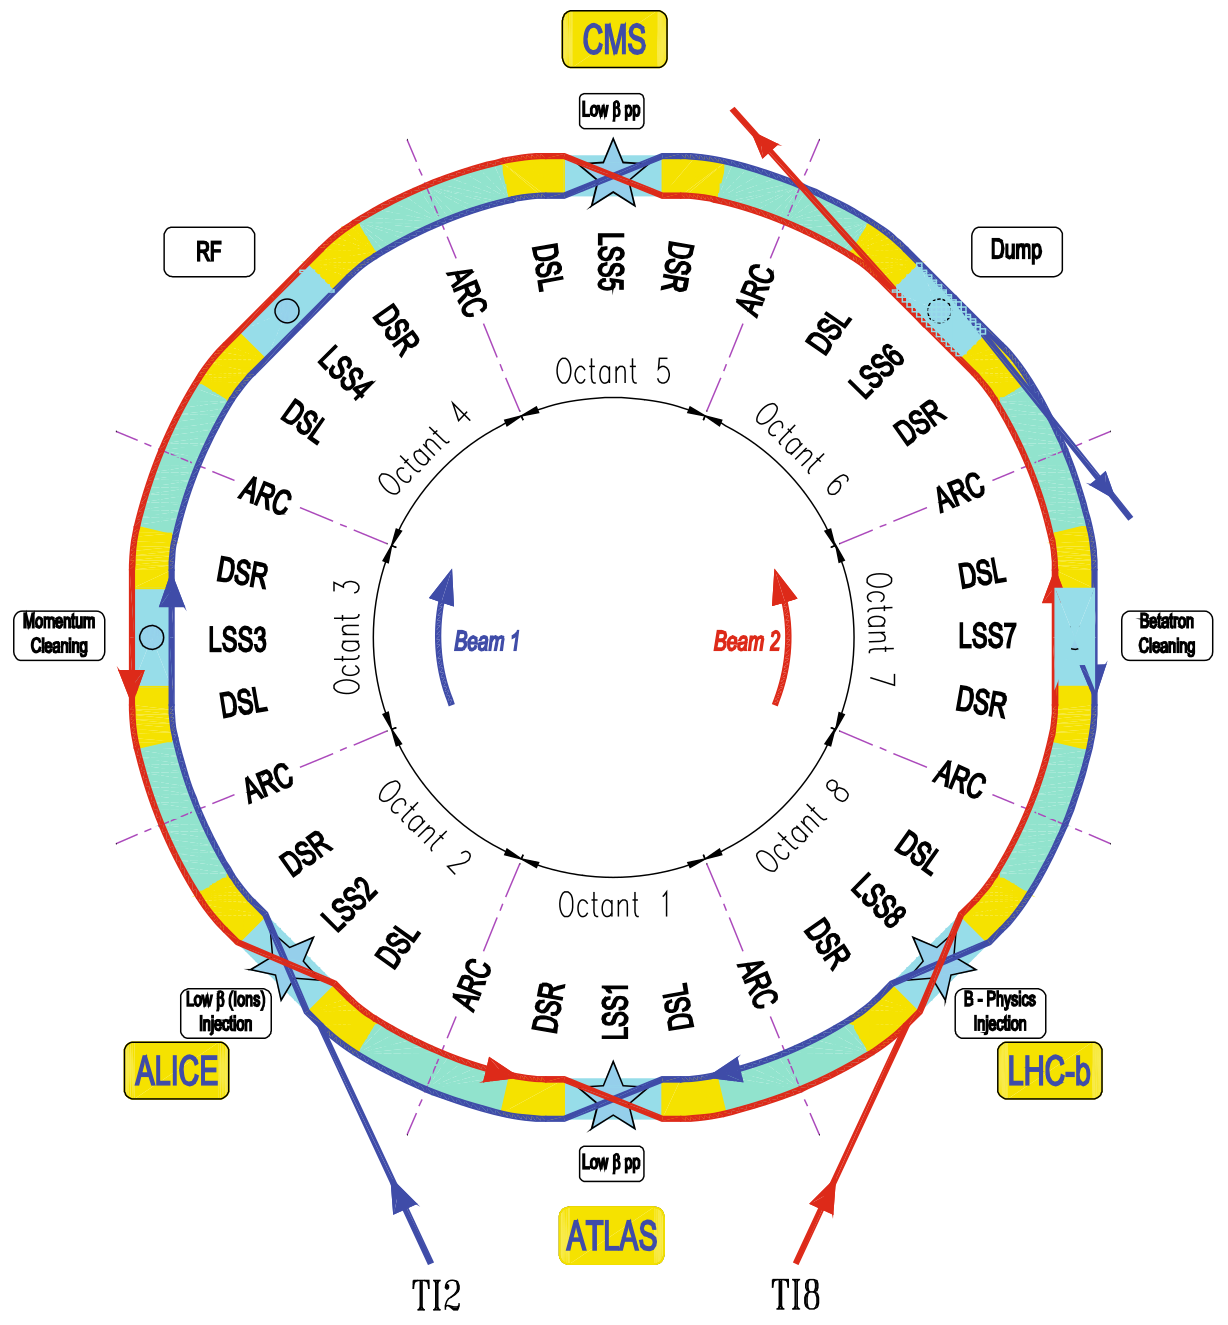
\includegraphics[width=0.49\textwidth]{5_Diffusion_measurement_LHC/figs/layout.png}
    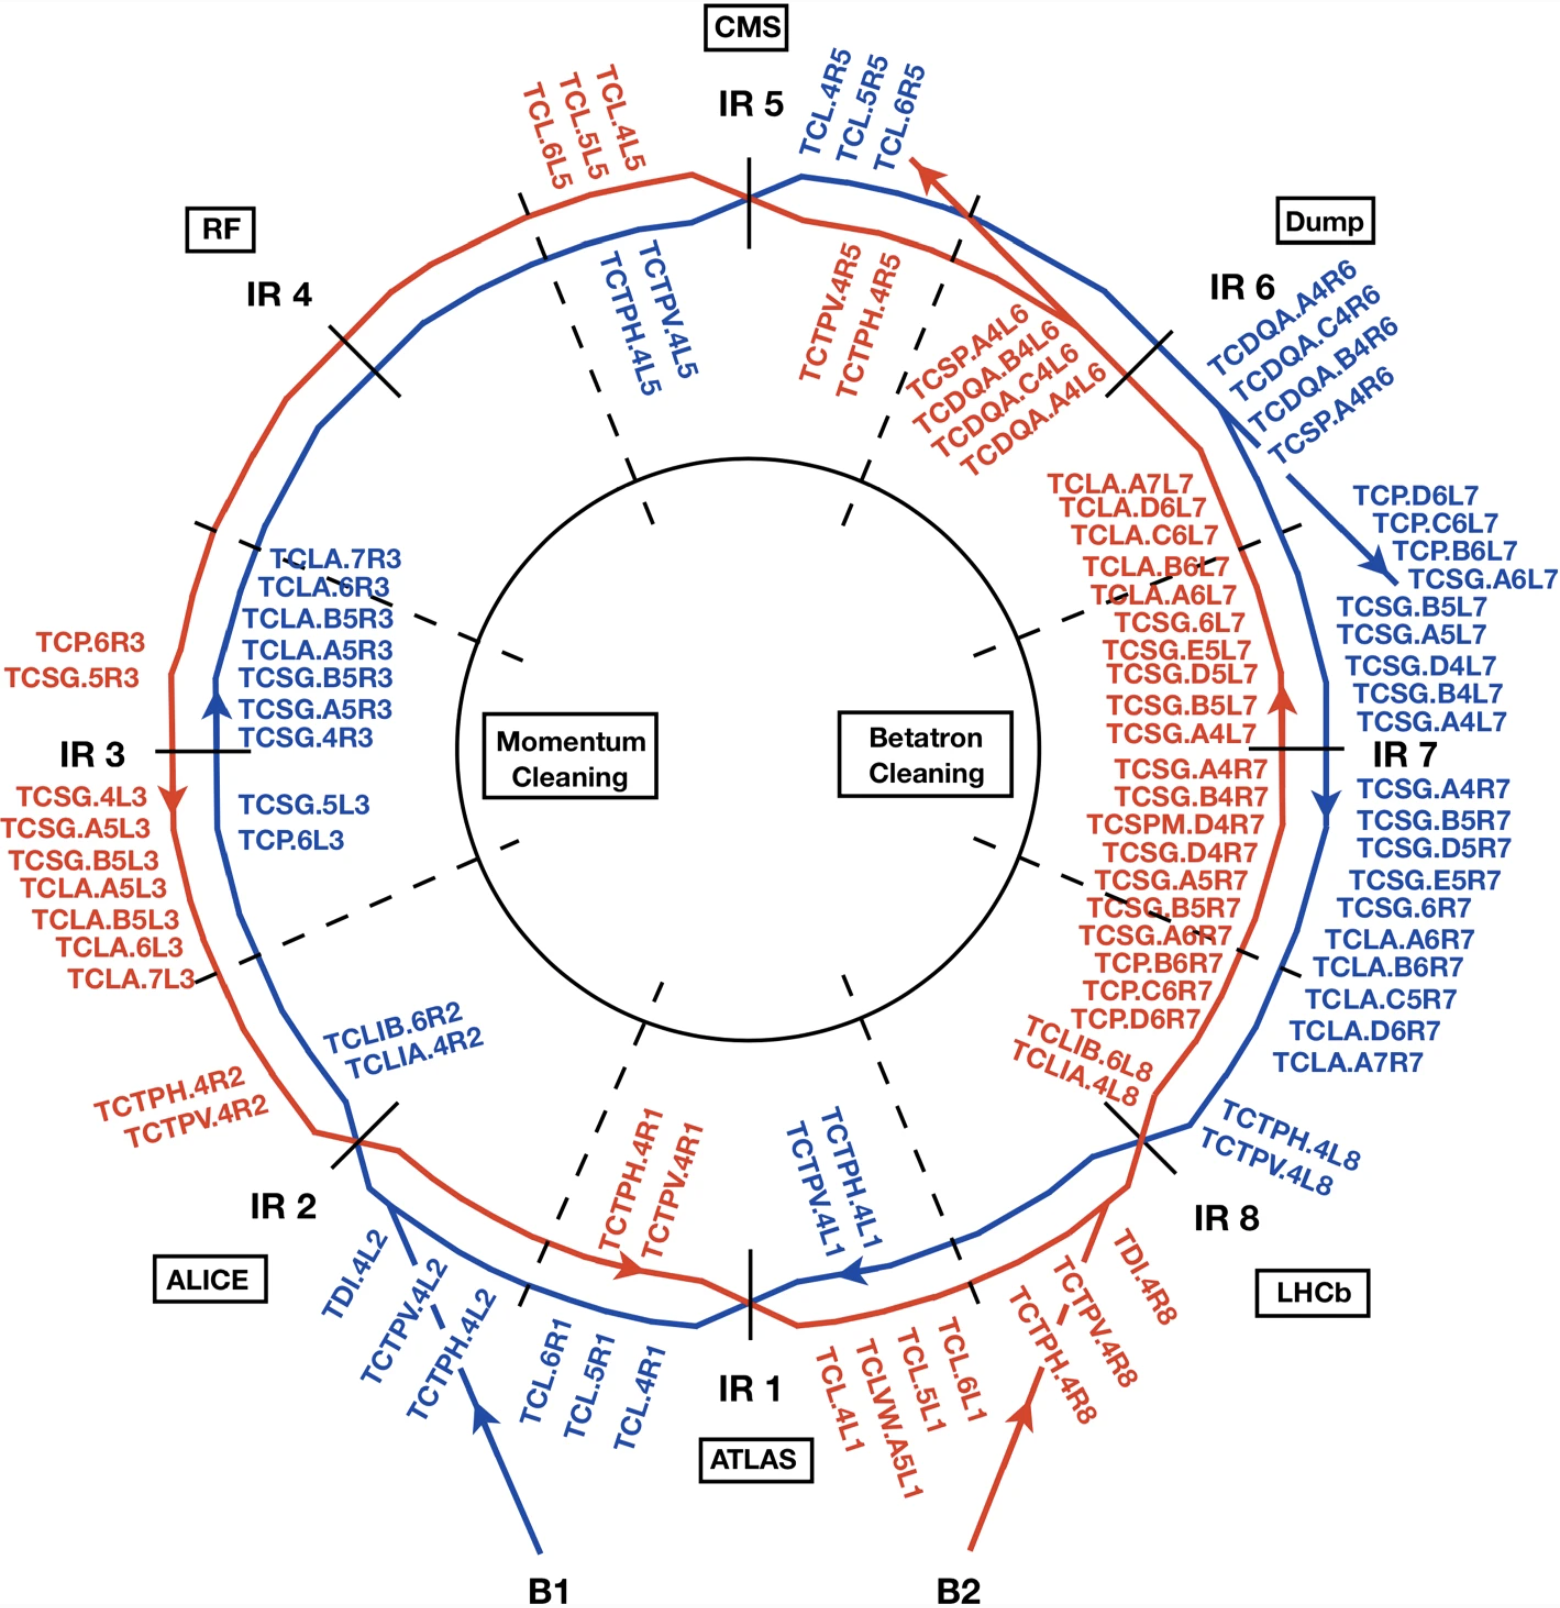
\includegraphics[width=0.49\textwidth]{5_Diffusion_measurement_LHC/figs/coll_scheme.png}
    \caption{Left, layout of the LHC. The ring follows an eightfold symmetry. Each octant hosts a Long Straight Sector (LSS) surrounded by two Dispersion Suppressor regions (DSR and DSL). Each octant is connected by an arc (ARC). (From Ref.~\cite{Bruning:782076}). Right, LHC collimation system layout in blue and red for Beam~1 and Beam~2, respectively. (From Ref.~\cite{azzopardi:crosstalk})}
    \label{fig:lhc_layout}
\end{figure}

The LHC collimation system is a fundamental component of machine operation and safety~\cite{1590664, Assmann:972336}. It has multiple functions, such as cleaning the beam halo, protecting the machine against unexpected and anomalous losses~\cite{BRUCE201719}, and reducing the background noise in experimental IPs~\cite{Bruce:1646958, Bruce:2686581}.

The collimation system counts more than 120 individual collimators. Most of these collimators are movable devices made up of two movable jaws made of solid material, which can be brought at different distances from the circulating beam~\cite{Bertarelli:794628}. A summary of the various collimators positioned along the LHC layout is reported in Fig.~\ref{fig:lhc_layout}, right. These jaws are straight and parallel to the beam and have a tapering at both ends, along the axis of the beam. The distance between the start and end of the tapering, where the jaw material is straight, is called the active length of the collimator. Some photos and schemes of these LHC collimators are reported in Fig.~\ref{fig:collimator_pics}.

\begin{figure}[hpt]
    \centering
    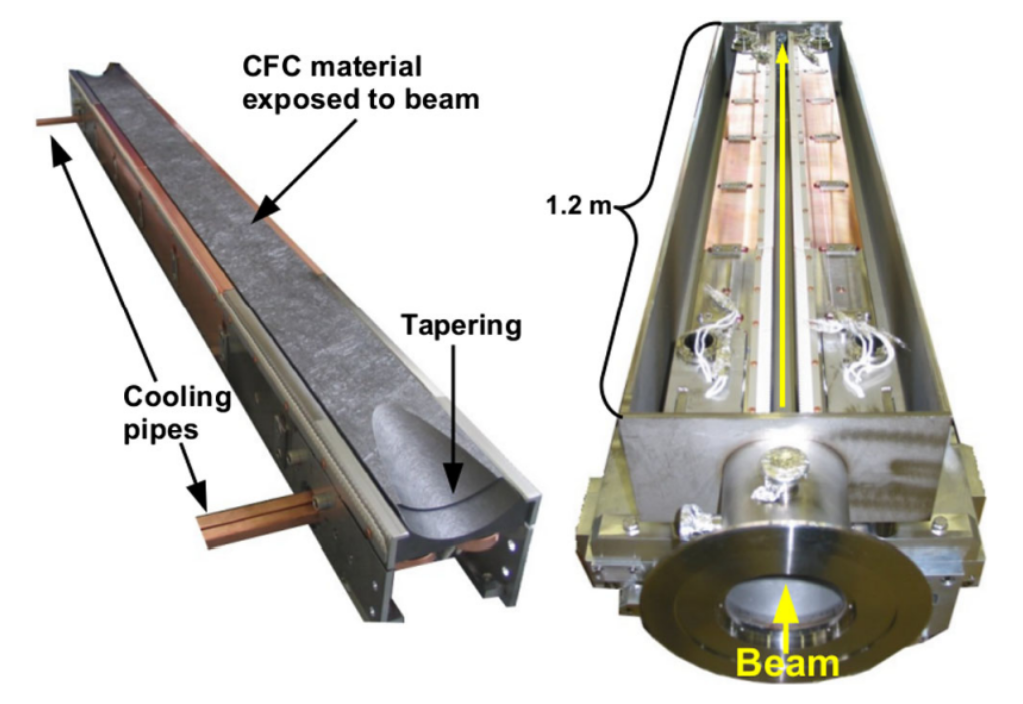
\includegraphics[width=0.75\textwidth]{5_Diffusion_measurement_LHC/figs/collimator_pics.png}
    \caption{Left picture, jaw of a secondary collimator, made of carbon-fiber composite (CFC) and water cooled through copper pipes. Right picture, two collimator jaws are installed in a collimator tank. (From Ref.~\cite{bruce2014simulations})}
    \label{fig:collimator_pics}
\end{figure}

At IR7, where the betatronic collimation system is located, we have an effective cleaning stage of halo particles that happen to have an excessively large amplitude of the betatron oscillation. This is called \textit{betatron cleaning}. To achieve effective betatron cleaning, we require that the magnetic lattice optics in the collimation region has very low dispersion and high $\beta$ function values. With such an optics setup, particles with high transverse displacement also feature high betatron displacement.

In IR3, instead, a \textit{momentum cleaning} of particles takes place. In that region, conversely, a high dispersion value is kept, so that the high transverse displacement is mainly caused by high momentum offset.

To safely clean the beam halo without damaging the magnets or other components of the machine, the LHC collimation system works on the basis of a multistage process. This multistage process consists of a \textit{hierarchy} of individual collimators with the purpose of progressively cleaning and controlling the loss of particles. A scheme of this hierarchy is presented in Fig.~\ref{fig:collimator_hierarchy}.

\begin{figure}[hpt]
    \centering
    \def\svgwidth{1.0\columnwidth}
    \import{5_Diffusion_measurement_LHC/figs}{hierarchy.pdf_tex}
    \caption{Scheme of the multistage collimation system in the LHC. The hierarchy includes primary (TCP), secondary (TCSG) and tertiary (TCT) collimators and shower absorbers (TCLA). Particles in the primary halo interact with the TCP and are scattered to the TCSGs. The hadronic showers coming from the TCSGs are finally absorbed by the TCLAs, and TCTs are in place to protect the aperture bottlenecks of the triplet quadrupoles. Part of the secondary halo interacts with the ionization chambers of the BLMs, and provide an indirect measurement of the primary halo. (Scheme based on Ref.~\cite{Hermes:2241364})}
    \label{fig:collimator_hierarchy}
\end{figure}

Primary collimators, which are also known as \textit{Target Collimator Primary} (TCP), are those placed closest to the edge of the beam and form the first stage of collimation. The purpose of this first collimation stage is to intercept and dispose of beam halo particles, i.e.\ it is the stage at which the beam halo actually gets intercepted above a certain threshold. When interacting with the primary collimator matter, the primary particles may exhibit various scattering behaviours, from acquiring an angular kick to depositing energy and producing secondary particles. 

These particles, scattered by the TCPs, form the secondary halo, which is then tackled by the secondary collimators \textit{Target Collimator Secondary-Graphite} (TCSG). The particles leaving the collimator finally form the tertiary halo, which finally interacts with the active absorbers, \textit{Target Collimator Long Absorber} (TCLA), which are installed downstream of the TCSGs, and \textit{Target Collimator Tertiarys} (TCTs), which make up a third final collimation stage for local protection for the aperture bottlenecks in the machine, i.e.\ in the triuplet quadrupoles.

Such a hierarchy offers various advantages over a simple single-stage collimation system. It ensures that particles that have been incorrectly outscattered at larger amplitudes and modified energies, constituting the so-called \textit{secondary beam-halo}, will be mainly absorbed by the next stages of collimation and not by other fragile parts of the machine. Moreover, the interaction of beam-halo particles with the primary collimator produces hadronic showers whose products can reach the cold magnets downstream of the cleaning region, possibly leading to unwanted quenches.

In IR7, there are 3 sets of collimators that cover the horizontal, vertical, and skew planes, as they have been shown to provide satisfactory cleaning~\cite{Jeanneret:368725}. The collimator hierarchies for these planes are, respectively, denominated by the letters C, D, and B. That is, the horizontal target primary collimator is called TCP.C. In IR3, the dispersion is only in the horizontal plane and only one set of collimators is installed to perform the longitudinal cleaning.

A multi-stage collimation system allows one to distribute the beam loads over a large controlled area. However, it also leads to a significant increase in the machine impedance, i.e.\ the level of self-interaction of the charged particle beam, mediated by the machine environment~\cite{Wiedemann2007}, which can be an important cause of beam instability and losses. Collimators are the single highest contributors of LHC impedance at top energy~\cite{Mounet:1451296}, as their resistive wall tends to be the element closest to the beam. Therefore, a multi-stage collimation system has to be configured so that it balances beam load distribution and impedance contributions efficiently. Active studies are ongoing to optimize the collimation system to minimize the beam losses and the machine impedance, see, e.g.\ Ref.~\cite{Antipov:2648423}.

The secondary particle showers represent the point of observation to measure the amount of primary particles absorbed by the TCPs. To quantify this amount, the LHC is equipped with multiple ionization chambers, which make up the beam loss monitor (BLM) system~\cite{blmSystem1, blmSystem2}. The charged particles that pass through the ionization chambers finally provide a measure of \SI{}{Gy \per s}, which can be converted into a corresponding measure of \SI{}{protons \per s} lost using a measured calibration factor, evaluated by controlled collimator-induced losses~\cite{arek}, which are also quantified in parallel by the \textit{DC Beam Current Transformer} (DCBCT)~\cite{Denard:1213275}, which measures the number of protons in the circulating beam by measuring the magnetic field, induced by the moving beam. A picture of an LHC BLM is presented in Fig.~\ref{fig:blm}. The calibrated BLM data are the precise loss signal that we finally expect to use to reconstruct the diffusion behaviour in the transverse plane.

\begin{figure}[hpt]
    \centering
    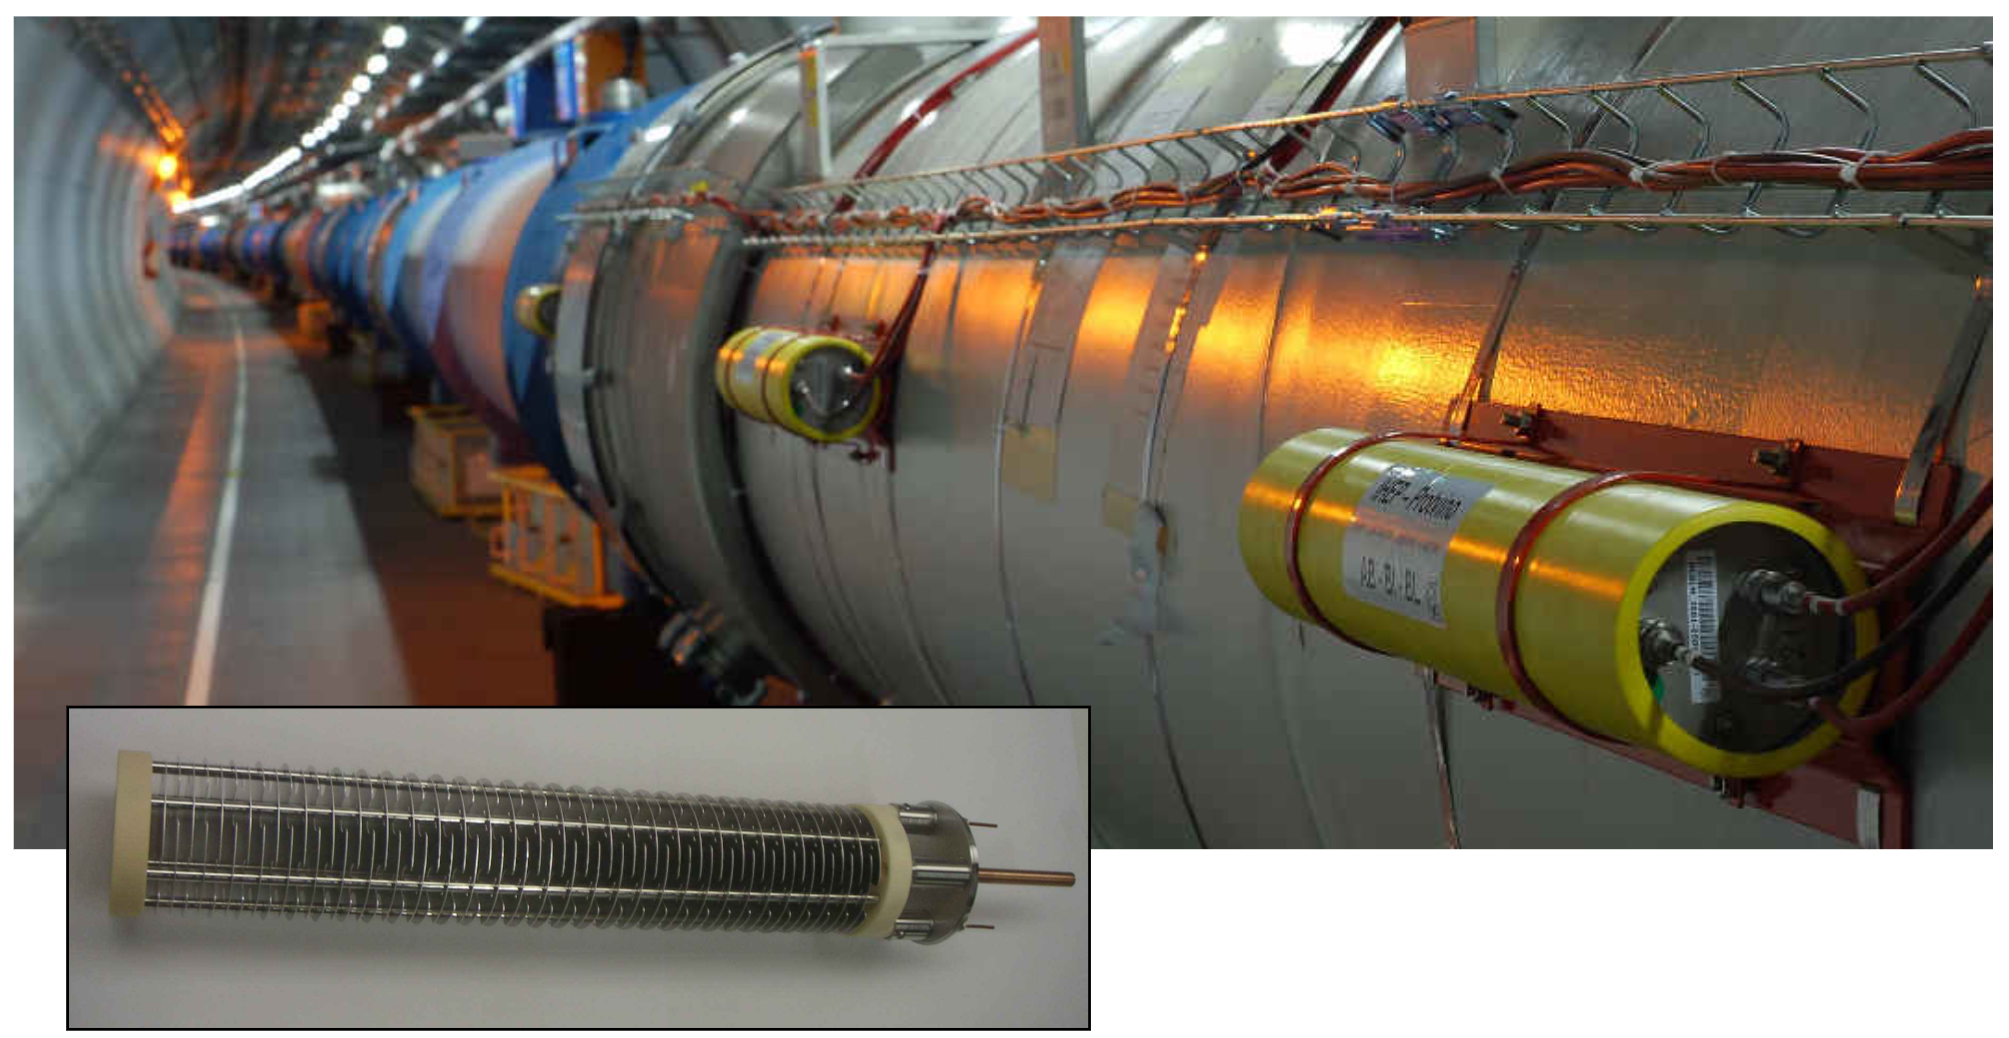
\includegraphics[width=0.75\textwidth]{5_Diffusion_measurement_LHC/figs/blm.png}
    \caption{Top picture, ionization chambers of the LHC BLM system, mounted on the side of the LHC Magnets. Bottom picture, inner structure of a BLM ionization chamber. (From Ref.~\cite{blmonline})}
    \label{fig:blm}
\end{figure}
%
\section{Analysis of experimental data}\label{sec:4:analysis}
%
Between 2016 and 2018, collimator scans were performed at the CERN LHC with physics beams at \SI{6.5}{TeV}~\cite{PhysRevAccelBeams.23.044802}. During these scans, one of the jaws of the primary collimators in IR7 was moved inward and outward in small steps, starting at $~5\sigma_\text{nom}$, where the nominal sigma value $\sigma_\text{nom}$ is evaluated for a nominal emittance $\varepsilon_\text{nom} =$ \SI{3.5}{\micro\meter}.

The scan was performed after executing a beam-based alignment~\cite{valentino2012semiautomatic} of the collimator, which is a procedure in which the TCP jaws are progressively positioned closer to the beam until the halo is touched. By performing such a procedure, one is sure that the centre of the collimator gap is precisely positioned around the local closed orbit.

The measurement is performed with the local beam loss monitoring (BLM) system and is provided in unit of \SI{}{Gy \per s} with \SI{1}{Hz} sampling rate, processed over different \textit{Running Sums} (RS), evaluated by a real-time processing system implemented on FPGA~\cite{4179157}. In this implementation, a time window is moved over the signal sampled by the device, and the maximum peak measured in the time window is considered the final measurement, which is finally reported in \SI{}{Gy \per s}, RSs range from a minimum of \SI{40}{\micro s} to a maximum of \SI{83.89}{s}. A list of the various RS defined in the measurement system is presented in Table~\ref{tab:rs_scheme}.

\begin{table}[hpt]
    \centering
    \scalebox{0.80}{
    \begin{tabular}{c|c|c|c|c|c|c}
    \toprule
        \multirow{2}{*}{\makecell{Signal\\Name}} & \multicolumn{2}{c|}{Time Windows} & \multicolumn{2}{c|}{Refreshing} & \multicolumn{2}{c}{Data formats} \\
        \cline{2-7}
        & \makecell{Number\\of \SI{40}{\micro s}\\steps} 
        & \makecell{Duration\\$[$\SI{}{ms}$]$} 
        & \makecell{Number\\of \SI{40}{\micro s}\\steps} 
        & \makecell{Duration\\$[$\SI{}{ms}$]$} 
        & FPGA/VME 
        & \makecell{Measurement\\and Logging DB\\(rate: \SI{1}{Hz})\\$[$\SI{}{Gy \per s}$]$}\\
        \midrule
        RS01 & $1$ & $0.04$ & $1$ & $0.04$ & \multirow{8}{*}{\makecell{Maximum of\\sum values\\observed\\from the\\last\\readout}} & \multirow{8}{*}{\makecell{Maximum of\\sums\\normalized\\to window\\length}} \\
        RS02 & $1$ & $0.08$ & $1$ & $0.04$ & & \\
        RS03 & $2$ & $0.32$ & $1$ & $0.04$ & & \\
        RS04 & $8$ & $0.64$ & $1$ & $0.04$ & & \\
        RS05 & $16$ & $2.56$ & $2$ & $0.08$ & & \\
        RS06 & $64$ & $10.24$ & $2$ & $0.08$ & & \\
        RS07 & $256$ & $81.92$ & $64$ & $2.56$ & & \\
        RS08 & $16384$ & $655.36$ & $64$ & $2.56$ & & \\
        \midrule
        RS09 & $32768$ & $1310.72$ & $2048$ & $81.92$ & \multirow{4}{*}{\makecell{\footnotesize Last calculated\\ \footnotesize sums observed\\\footnotesize in the last\\\footnotesize readout}} & \multirow{4}{*}{\makecell{\footnotesize Last calculated\\\footnotesize sum normalized\\\footnotesize to window length}} \\
        RS10 & $131072$ & $5242.88$ & $2048$ & $81.92$ & & \\
        RS11 & $524288$ & $20971.52$ & $16384$ & $655.36$ & & \\
        RS12 & $2097152$ & $83886.08$ & $16384$ & $655.36$ & & \\
    \bottomrule
    \end{tabular}
    }
    \caption{Specifications of the various Running Sums (RSs) that are defined in the FPGA based data gathering system of the BLMs. (Ref.~\cite{rsdeftable})}
    \label{tab:rs_scheme}
\end{table}

\begin{figure}[hpt]
    \centering
    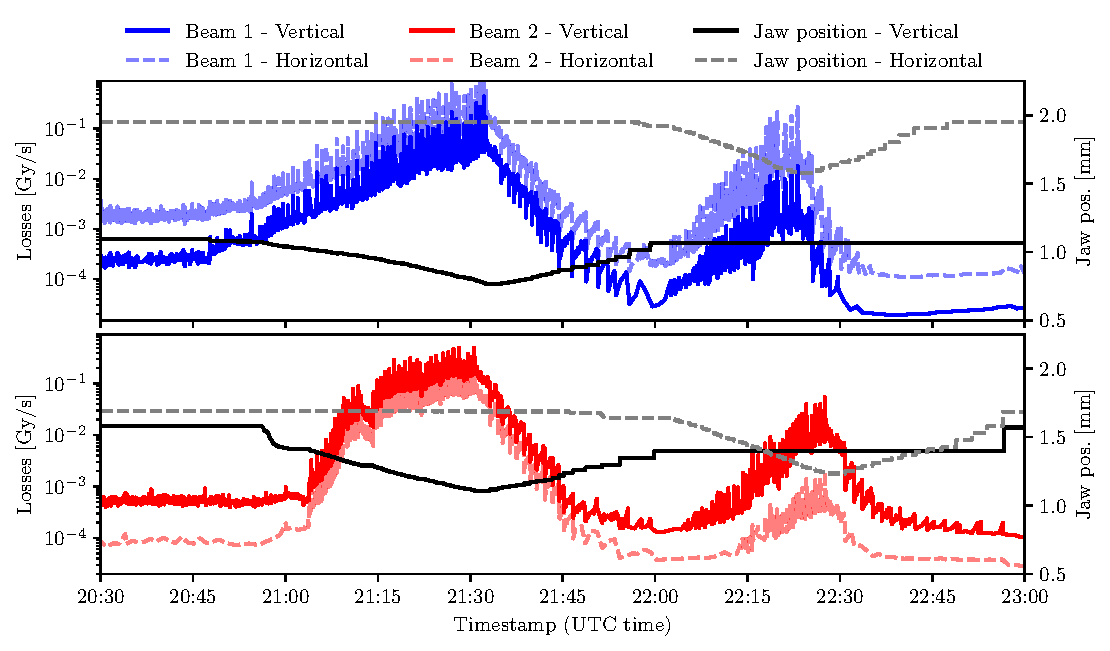
\includegraphics[width=\textwidth]{5_Diffusion_measurement_LHC/figs/raw.pdf}
    \caption{Beam loss data from the two separate BLM monitors corresponding to the TCPs on the vertical and horizontal planes, using RS06 (i.e.\ the maximum spike over a time window of \SI{10.24}{ms}), for Beam~1 and Beam~2, and positions of IR7 TCP jaws measured in the vertical and horizontal plane for the collimator scans carried out in fill 6052. The data acquired represent a complete collimator scan on both planes. The jaw positions are considered from the beam centre position, measured after a beam-based alignment. (Data from Ref.~\cite{PhysRevAccelBeams.23.044802})}
    \label{fig:raw_data}
\end{figure}

The IR7 TCPs dedicated to the vertical plane and to the horizontal plane (namely, TCP.D and TCP.C) were used to perform a collimator scan of the beam halo on both Beam~1 and Beam~2, performing a sequence of inward steps, with pauses of a few seconds between each step, followed by a train of outward steps, with pauses ranging from $\sim30$ seconds to almost two minutes between steps. The scraping was first performed on the vertical plane and then on the horizontal plane. 

During the scraping, the BLM data were recorded by the ionization chambers placed after the collimator hierarchy. Two dedicated sets of BLMs are placed for the two separate planes and are considered in our analysis depending on the plane that is undergoing scraping. In Fig.~\ref{fig:raw_data} we present the data collected during fill 6052 of type RS06, i.e.\ sampling the maximum spike measured by the BLM over a time window of \SI{10.24}{ms}. Here, the collimator jaw positions are reported in millimetres from the centre of the beam, measured after the beam-based alignment. The two different BLM planes reading is reported.

It should be noted that these collimator scans were not performed using an optimal protocol such as that proposed in the previous chapter. In fact, complete inward scans, followed by outward scans, were used instead of a sequence of in/out steps. Furthermore, jaw movements were not always performed leaving enough time for the system to relax to its equilibrium state. This can be observed from the fact that, between most outward steps, the loss signal still has a non-negligible positive first derivative when the next collimator outward step is performed, suggesting that a recovery current process was still ongoing when the jaw was moved, as the expected global current process has negative or close to zero first derivative. This suggests that an ideal resting time between steps was not archived before the next collimator step.

Due to these two characteristics of the measurement protocol used during the collimation scan, some of the working hypothesis made in the previous chapter, which ultimately allow the reconstruction of $D(I)$ by fitting the normalized recovery current, may not hold. More specifically, we lack the upper bound to reconstruct the global current, and we cannot be sure that the beam tail distribution after an outward step follows Eq.~\eqref{eq:outward_difference}.

To address these characteristics and shortcomings of the data, we had to consider only a subset of the data and modify some of the elements of the fitting procedure. 

To address the lack of alternating jaw movements, we selected a region of interest (ROI) in which many outward steps were performed with almost regular sampling, with loss signals exhibiting the features we expect to see from a recovery current. This decision is motivated by the fact that the simulation study presented in the previous chapter shows how recovery currents induced by outward steps are much more reliable for reconstruction purposes than those induced by inward steps. 

In Fig.~\ref{fig:first} we present the portion of the data collected in Fill 6052 that we finally selected. Unfortunately, only the scraping performed in the vertical plane meets our quality requirements to apply the fitting of our diffusive model.

\begin{figure}[hpt]
    \centering
    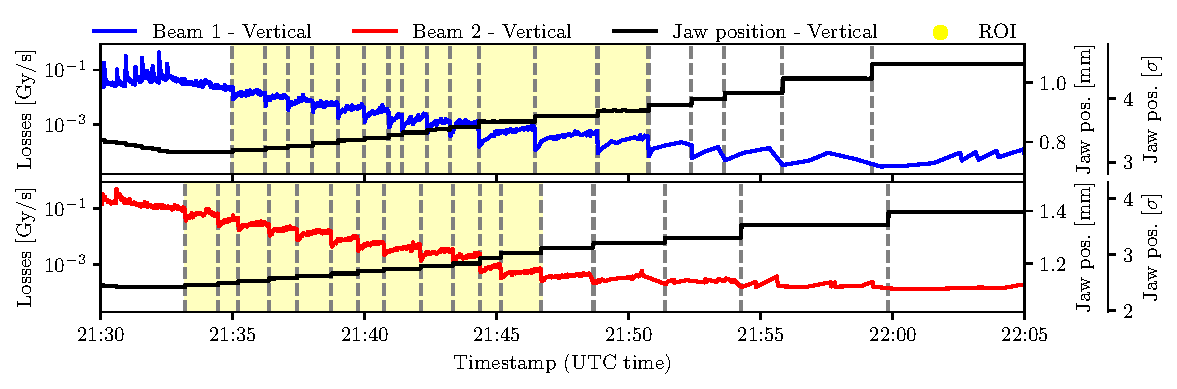
\includegraphics[width=\textwidth]{5_Diffusion_measurement_LHC/figs/first.pdf}
    \caption{Selected data from Fill 6052 (i.e.\ Fig.~\ref{fig:raw_data}). The data shown correspond to outward jaw movements in the vertical plane. The yellow-marked region of interest (ROI) represents a subset of data meeting our quality requirements for applying the fitting of our diffusive model. The jaw positions are considered from the beam centre position, measured after a beam-based alignment. A corresponding position measured in $\sigma$ units is also reported. (Data from Ref.~\cite{PhysRevAccelBeams.23.044802})}
    \label{fig:first}
\end{figure}

The measured collimator jaw position is converted to measured beam sigma units $\sigma$ using the nominal optical parameters and the measured value of the beam emittance, taking into account the position of the beam centre. The nominal optical parameters were considered as the measured $\beta$-beating level, i.e.\ the difference between the measured optical functions and the expected nominal values, was in the few percent level as expected from regular LHC operation~\cite{PhysRevAccelBeams.20.054801}.  To convert the \SI{}{Gy \per s} units of the BLM signal to \SI{}{protons \per s}, we used a calibration factor $F$~\cite{arek} dependent on the TCP jaw position. This calibration factor $F$ is calculated from the BLM loss data and the intensity lost recorded by the DCBCTs during the collimator steps. The coefficient reads 
\begin{equation}
    F = \left(-9.0\times10^{-14}\sigma + 6.2\times10^{-13}\right)^{-1} \,,
\end{equation}
where $\sigma$ is the position of the collimator jaw in sigma units.

The absence of alternating jaw movements implies a lack of information for constructing an upper-bound estimate of the global current. Moreover, since the jaw movements were not always performed to allow enough time for the system to relax to its semi-stationary state, we cannot make strong assumptions on the global current value by only interpolating the end points of the outward recovery currents. 

To address this issue, we define an initial estimate of the global current shape $J_\text{eq}^{\text{est}}(t)$, by constructing a Cubic Spline Interpolation (CSI) passing through the end points of the sequence of outward recovery currents, following the same methodology as presented in the previous chapter. This ``fundamental CSI'', has the features we expect to observe from a global current we expect to observe from a Nekhoroshev-like Fokker-Planck process. However, by just interpolating the end points, it does not take into account missing recovery due to collimator steps being performed too quickly.

To include this missing information, the fundamental CSI has been multiplied by different constant terms to represent possible different levels of partial recovery of $J_\mathrm{R}(t)$. This procedure is shown in Fig.~\ref{fig:second}. One can see how the fundamental CSI represents the initial lowest estimate of global current, while the different multiplicative constants introduce different gap levels after the terminating points of the recovery currents. This multiplicative can then be treated as a free parameter for reconstructing missing information.

%
\begin{figure}[hpt]
    \centering
    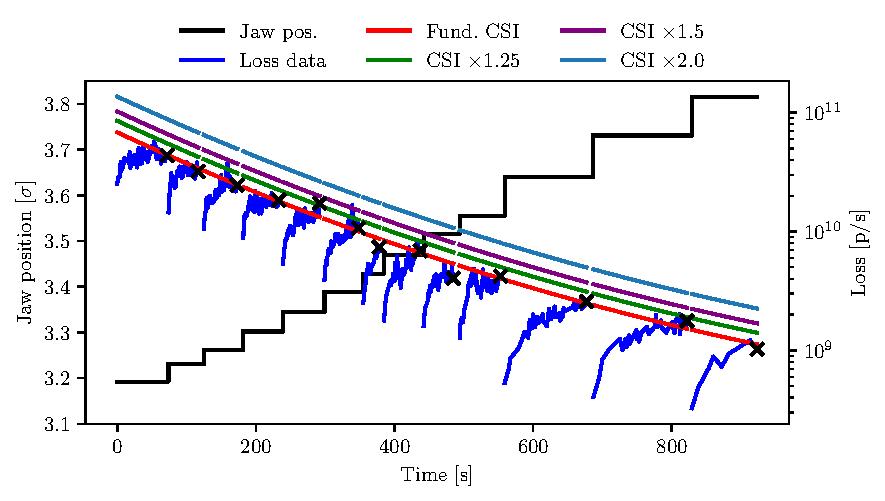
\includegraphics[trim={0 2.5mm 0 3mm}, clip, width=\columnwidth]{5_Diffusion_measurement_LHC/figs/second_bis.pdf}
    \caption{Possible estimates of $J_\mathrm{eq}(t)$ for Beam~1 data. An initial estimate is made starting from a Cubic Spline Interpolation (CSI) with positive second derivative passing through the end points of the measured recovery currents (red line). The various curves are obtained by multiplying the fundamental CSI by a constant term, and represent estimates of the partial recovery currents. The multiplicative constant considered is reported in the plot legend.}
    \label{fig:second}
\end{figure}
%

Finally, the rapid sequence of jaw movements introduces another issue: the difference distribution $\rho^\ast$ cannot be described with certainty by Eq.~\eqref{eq:outward_difference}, or its approximated form by Eq.~\eqref{eq:outward_difference_approx}. To address this issue, we replace the $D(I)$-dependent integral terms in Eq.~\eqref{eq:outward_difference_approx} with the approximation
\begin{equation}
    \rho_{\mathrm{app}}^{\ast}(I)= \begin{cases} -M & \text { if } I\leq I_{\mathrm{a}}\\ -\left(\frac{I_{\mathrm{a}}^{\prime }-I}{I_{\mathrm{a}}^{ \prime}-I_{\mathrm{a}}}\right) M & \text { if } I>I_{\mathrm{a}}  \end{cases} \, ,
    \label{eq:approximated_distribution_beam}
\end{equation}
where $M$ is a fixed constant for each jaw movement that represents an unknown amount of out-of-equilibrium distribution.

A scan is performed on different combinations of the multiplicative factor of the CSI and of $M$, while keeping track of the $\chi^2$ achieved by the fitting routine that determines the values of the model parameters $\kappa, I_\ast$. The result of this procedure is shown in Figs.~\ref{fig:fourth} and~\ref{fig:fifth}, where one can observe the existence of an optimal configuration of parameters and the good reconstruction performance achieved by such a configuration. The optimal fit results for Beam~1 and Beam~2 data are reported in Table~\ref{tab:fit_results}.

\begin{figure}[hpt]
    \centering
    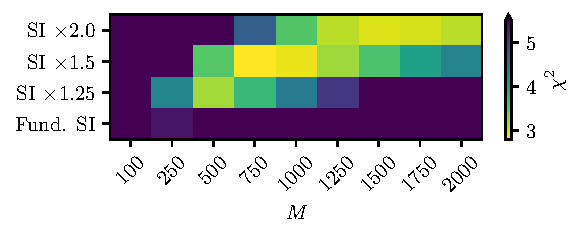
\includegraphics[trim={0 2.5mm 0 1.5mm}, clip, width=0.98\columnwidth]{5_Diffusion_measurement_LHC/figs/fourth.pdf}
    \caption{Fit performance of $\kappa$ and $I_\ast$ for Beam~1 data, using different combinations of CSI multiplicative constants and values of $M$ for Eq.~\eqref{eq:approximated_distribution_beam}. The color map shows the existence of an optimal pair of values at (CSI $\times 1.5$, $750$).}
    \label{fig:fourth}
\end{figure}
%
\begin{table}[hpt]
    \centering
    \begin{tabular}{lcccc}
        \toprule
        Beam / Plane & CSI & $M$ & $\kappa$ & $I_\ast\ [\sigma]$ \\
        \midrule
        Beam~1 / V & $\times1.5$ & $750$ & $0.59\pm0.03$ & $21\pm2$ \\
        Beam~2 / V & $\times1.5$ & $1000$ & $0.85\pm0.02$ & $39\pm8$ \\
        \bottomrule
    \end{tabular}
    \caption{Results of the fit procedure of $\kappa$ and $I_\ast$ for the selected data in the vertical plane, along with corresponding setup obtained for the CSI multiplicative constant and $M$ value for \eqref{eq:approximated_distribution_beam}.}
    \label{tab:fit_results}
\end{table}
%

Note that the values reported in~\cite{bazzani2020diffusion}, namely $\kappa=0.33 $ and $I_\ast \simeq 21$, were obtained for Beam~2 and considering the diffusion in the vertical plane. It should be stressed that these previous measurements were performed with non-colliding bunches, whereas in the beam measurements analysed here, beam-beam effects were present.

\begin{figure}[hpt]
    \centering
    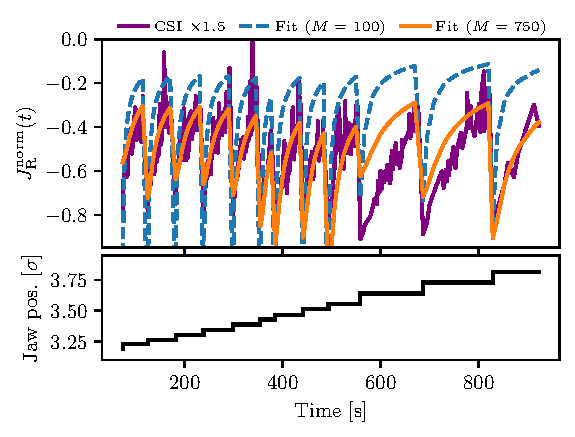
\includegraphics[trim={0 2.5mm 0 3mm}, clip, width=0.95\columnwidth]{5_Diffusion_measurement_LHC/figs/fifth.pdf}
    \caption{Fit results for Beam~1 data for two $M$ values, considering the recovery current obtained by using the optimal CSI multiplicative constant $\times 1.5$. The optimal $M$ value (orange) outperforms a lower $M$ value (blue) and manages to reconstruct the shape of the recovery currents.}
    \label{fig:fifth}
\end{figure}
%
\section{Final remarks}\label{sec:4:remarks}
%
Despite the differences between the approach used to collect the data during LHC Run~2 and the optimal one suggested by the numerical studies performed on the Nekhoroshev-like Forkker-Planck diffusive model, we were able to analyse the loss signal measured by the BLMs during collimator scans, and obtain a promising reconstruction of the recovery currents, which are ultimately the indicator of diffusive-like behaviour.

To address missing information in the data, due to the different measurement protocol used, we had to adapt some of the key elements of our fitting procedure. That is, we had to define a new method for reconstructing the global current estimate and we had to consider a different form for the difference distribution $\rho^\ast$. This led to good reconstruction performances and promising insights into the global diffusive behaviour of the LHC beam halo.

Future collimator scans during the LHC Run~3 will focus on acquiring beam data using the proposed optimized experimental method, to characterize more accurately the presence of non-linear diffusive behaviour. 

\chapter{Diffusive model application on wire compensators losses}

\section{LHC beam-beam wire compensators fundamentals}

One of the most significant limits in the present LHC design and future HL-LHC design is given by the electromagnetic interactions between the two counter-rotating beams in the shared sections of the machine, the interaction points~\cite{Arduini_2016}. These interactions lead to the so-called \textit{beam-beam effects}, and can be distinguished as head-on beam-beam effects, which occurs when the beam bunches are overlapping in the interaction point, and long-range beam-beam effects, caused by having the two beams close together for the whole length of the shared region.

In the LHC, the beams are set in collision with a small \textit{crossing angle}, which has both the purpose of separating bunches immediately upstream and downstream of the collision point~\cite{Arduini_2016} and to reduce the presence of long-range beam-beam effects, since smaller angles imply smaller beam separation. However, an increase in crossing angle also implies a reduction in integrated luminosity, that is, the total number of collisions that have occurred over a given period of time, typically measured in inverse femtobarns \SI{}{fb}$^{-1}$~\cite{Herr:941318}, as the bunches overlap decreases. A schematic visualization of two different crossing angles and their consequent effect on beam separation and bunch overlap is presented in Fig.~\ref{fig:crossing-angles}. The nominal full crossing angle for the LHC is set at $\theta_c =$ \SI{285}{\micro\radian}, while for HL-LHC the expected baseline parameter will be set at $\theta_c =$ \SI{500}{\micro\radian}~\cite{BejarAlonso:2749422}. 

\begin{figure}[hpt]
    \centering
    \def\svgwidth{1.0\textwidth}
    \import{5_wire_compensators_LHC/figs/}{crossing_angle_basics.pdf_tex}
    \caption{Schematic visualization of two different crossing angles and their consequent effect on beam separation and bunch overlap. As $\theta_{c1} > \theta_{c2}$, the bunches are more separated in the first case (left), while the bunch overlap is larger in the second case (right). The long-range beam-beam effects are also more significant in the second case.}
    \label{fig:crossing-angles}
\end{figure}

To address long-range beam beam effects, while maintaining a small crossing angle, a corrective approach based on electromagnet lenses was presented in~\cite{Koutchouk:692058}. The core concept of this approach is to compensate for the perturbation pattern given by long-range effects by using DC wires. The idea of using DC wires specifically comes from the observation that these long-range effects were similar to the $1/r$ dependence similar to the electric field potential given by a simple wire~\cite{PhysRevSTAB.5.074001}. A sketch of the concept of compensation given by the BBCW is presented in Fig.~\ref{fig:wire-baseline}.

\begin{figure}[hpt]
    \centering
    \def\svgwidth{1.0\textwidth}
    \import{5_wire_compensators_LHC/figs/}{crossing_angle_kick.pdf_tex}
    \caption{Left, sketch of the long-range beam-beam effects felt by Beam~2 from Beam~1, following the weak-strong approximation (i.e.\ we consider the effect of Beam~1 on Beam~2 and not vice versa). Right, sketch of the principle of the compensation given by the BBCW. The long-range beam-beam effects (red arrow) are compensated by the DC wires (green arrow), which are placed in the beam path before and after the interaction point.}
    \label{fig:wire-baseline}
\end{figure}

The resulting tool is referred to as \textit{``beam-beam wire compensator''} (BBCW), and it has been tested in multiple iterations on various accelerator complexes (a complete list of experimental applications up to early 2022 is available in~\cite{axel.wires}).

In the LHC, the BBCW are installed for Beam~2 only, as it was the only beam that was expected to operate with a coronograph~\cite{Goldblatt:2313940}, which is a device that is expected to allow transverse beam halo measurements in the future. The wires are embedded in the tertiary collimators placed before and after IP1 and IP5~\cite{Rossi:2696270}. These collimators are still part of the collimator hierarchy, presented in Section~\ref{sec:collimation}, with the primary and secondary components placed in IR3 and IR7, and are placed near the IPs to locally protect the experiments from potentially damaging losses.

A collimator hosts two separate wires (one per jaw), and each wire can carry up to \SI{350}{\ampere}. These two separate wires are cabled in series so that they have the same polarity. This configuration enables a specific 2-jaw powering setup with the characteristics of doubling the odd multipolar strength of the kick, while the even ones cancel out. This choice is motivated by the need to compensate for octupolar resonances~\cite{Poyet:2703503}. The two possible configurations are presented in Fig.~\ref{fig:wire-configs}. The first one, called the \textit{single wire} configuration, only powers up the internal wires. The second one, referred to as \textit{quadrupolar configuration}, powers up both wires.

\begin{figure}[hpt]
    \centering
    \def\svgwidth{1.0\textwidth}
    \import{5_wire_compensators_LHC/figs/}{crossing_angle_configs.pdf_tex}
    \caption{Left, sketch of the single wire configuration, where only one wire per pair is powered up. Right, quadrupolar configuration, where both wires in the pairs are powered up to compensate the octupolar resonances.}
    \label{fig:wire-configs}
\end{figure}

\section{Overview of experimental data}

For the application of our diffusive framework, we consider the experimental data gathered at the CERN LHC during the 2018 LHC Machine Development (MD) programme, during the BBCW measurements campaign~\cite{Poyet:2703503}. More specifically, we consider the data gathered during fill 7386, as it has the configuration closest to an operational scenario.

During this MD measurement, the BBCW prototypes installed for Beam~2 were tested in various long-range beam-beam dominated scenarios. Starting from low intensity fills for validating the BBCW configuration, up to high-intensity fills, such as the one we are considering. 

During fill 7386, three trains of symmetric bunches were tested at flat top energy with beams colliding at different crossing angles, smaller than the nominal one in order to have strong long-range beam-beam effects. During this operational-like fill, the wire compensators were set in the quadrupolar configuration. The loss signals measured by the BLMs for the two beams are shown in Fig.~\ref{fig:wire-data}, note that the measurement unit is in \SI{}{protons \per s}, as we are considering calibrated losses. Along with the BLM data, the beam intensity measured by the BCTs, the wire power, the octupole power, and the crossing angles are also reported. 

\begin{figure}[hpt]
    \centering
    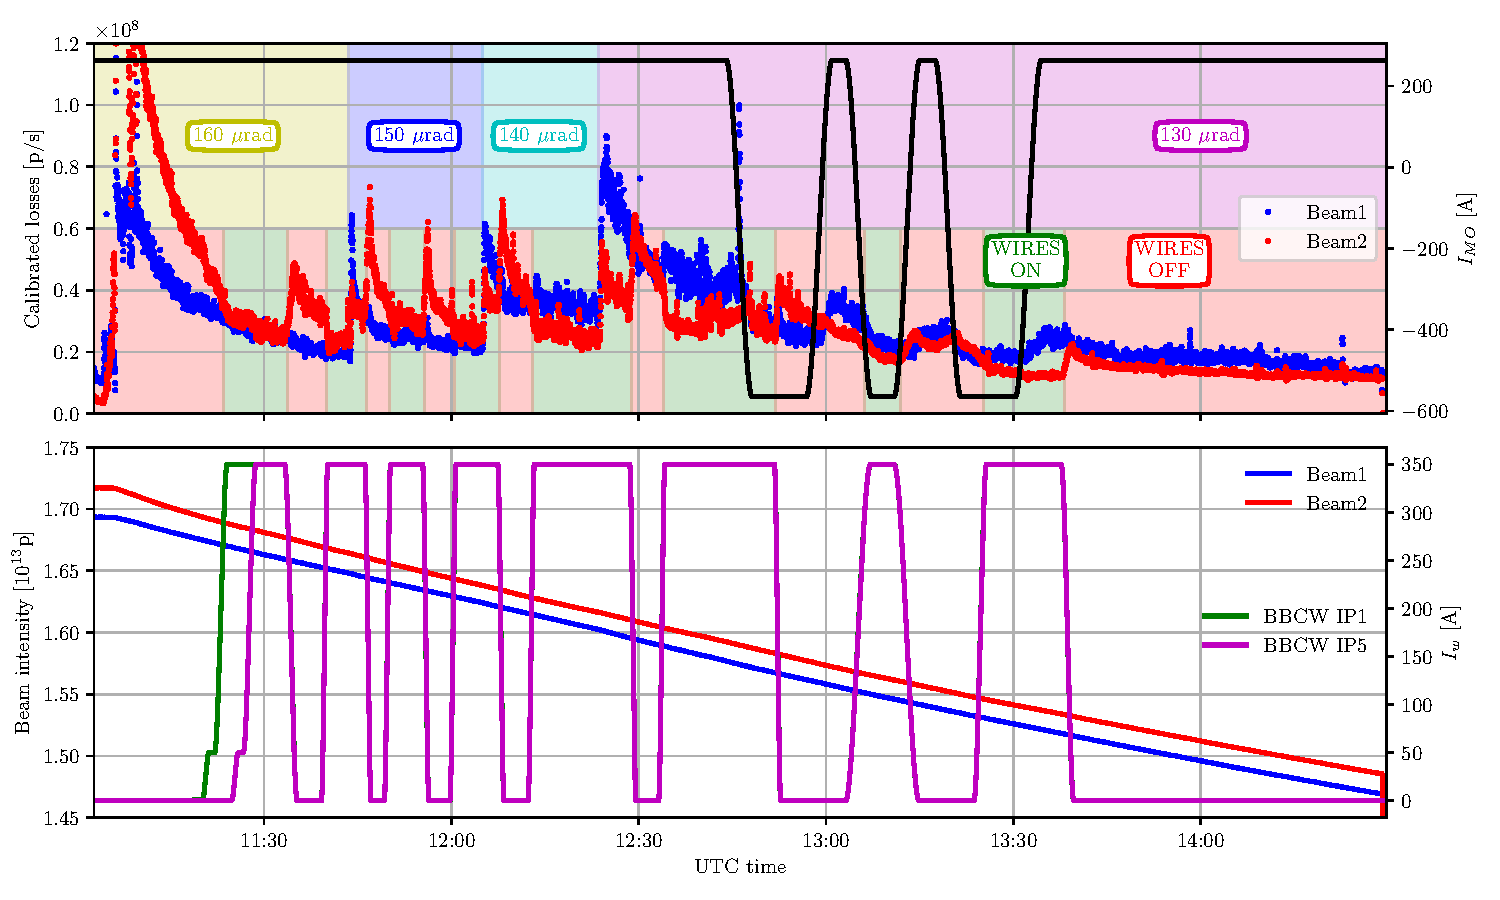
\includegraphics[width=1.0\textwidth]{5_wire_compensators_LHC/figs/wire_summary.pdf}
    \caption{Overview of the data gathered during fill 7386. BLM calibrated losses and BCT beam intensity measurements were taken at different combinations of crossing angles, wire power, and octupole power.}
    \label{fig:wire-data}
\end{figure}

The BLM data for Beam~1 and Beam~2 in units of \SI{}{protons \per s} represents a high-precision measure of protons lost over time. Instead, the BCT data provide a measurement of the intensity of the beam in number of protons over time. Such measurement is not particularly precise, and, qualitatively, it can be seen from the plot how the intensity measured does not distinguish the different regimes of losses highlighted by the BLM data, and maintains a steady linear decrease. This difference in precision makes the BLM data a fundamental tool for inspecting the different regimes of losses in the transverse plane.  

BBCW and octupole magnets power state is reported in Ampere units.  BBCW wires can be found in either an \textit{off} state, namely at \SI{0}{\ampere}, or in an \textit{on} state, namely at \SI{350}{\ampere}. Instead, the octupoles are found at two different amperage values, namely $260$ and \SI{-560}{\ampere}. It is important to highlight how the switch of state for both systems is not instantaneous but requires instead a non-negligible amount of time; this will be thoroughly discussed in the next section.

It is possible to see how the data provide a various number of crossing angle configurations, along with on-off alternations of both BBCW power and octupoles current. Qualitatively, one can see how the BBCW equipped in Beam~2 do lead to a lower BLM loss signal when they are turned on, while turning them off leads to a strong peak in the losses measured by the BLMs.

We will now discuss how our diffusive framework can be applied to this loss signal, along with some necessary considerations on how one must preprocess and interpret these data, before applying the model. 

\section{Application of the diffusive model}

Let us consider the Fokker-Planck equation presented in Eq.~\eqref{eq:fp}, with the Nekhoroshev-like functional diffusion coefficient of Eq.~\eqref{eq:diffusion}. We recall that the system is fully characterized by the three free parameters $\epsilon$, $I_\ast$, and $\kappa$.

To apply this model to the BLM data and reconstruct $D(I)$ for the various states of the system, we perform a fitting approach inspired by the procedure used in the work of Bazzani et al.~\cite{bazzani2020diffusion}, where the same Fokker-Planck model is used to reconstruct the normalized intensity of the beam, evaluated over the number of turns.

Starting from the BLM and BCT data we have at hand, we want to construct a measure of the normalized intensity of the beam over the number of turns. To archive this, we first convert the measurements from seconds to the number of turns, considering that in LHC Run2, a reference proton at \SI{6.5}{TeV} performs 11245 turns every second. To then evaluate the relative intensity lost over an interval $[N_0, N_1]$, as the BCT data are not precise enough to highlight fine differences in loss rates, we consider as the amount of protons lost the integrated BLM signal, and we take the BCT value registered at $N_0=3.5\times10^6$ turns as the reference intensity, as it is the moment at which the first peak in BLM losses was measured. This procedure is illustrated in Fig.~\ref{fig:blm-to-intensity}.

\begin{figure}[hpt]
    \centering
    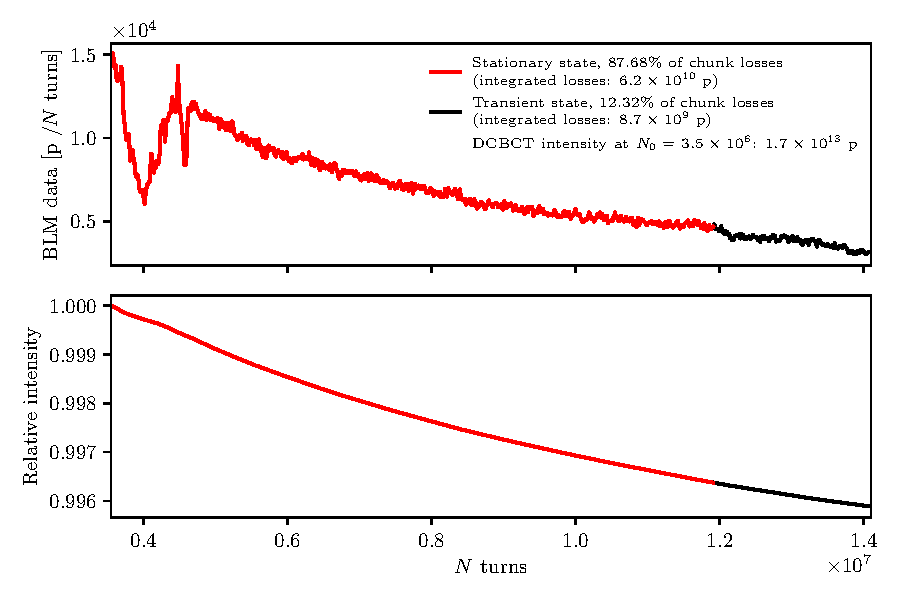
\includegraphics[width=1.0\textwidth]{5_wire_compensators_LHC/figs/stationary_transient_example_chunk.pdf}
    \caption{Example of the procedure used to evaluate the relative intensity lost over an interval $[N_0, N_1]$. The BLM signal is integrated over the interval, and the BCT value registered at $N_0=3.5\times10^6$ turns is used as the reference intensity. A comparison between the integrated losses measured in the stationary state of the chunk and the transient state is also reported. As the losses in the transient state are much lower than the losses in the stationary state, our working hypothesis still holds.}
    \label{fig:blm-to-intensity}
\end{figure}

Along with the various assumptions made to enable the application of the Nekhoroshev estimate, such as the averaging principle on the angular variables, it is important to note that this model has the strong hypothesis that $D(I)$ does not evolve over time. This implies that the magnetic lattice of the accelerator must not manifest stronger variations than the ones given by the small stochastic perturbation. Such a strong assumption requires some preliminary consideration on the BLM loss signal we have at hand.

When the BBCW, the crossing angle, and the octupoles are in a stationary state, we can state that the parameters of the Fokker-Planck equation can be considered as constant over time, since the magnetic lattice does not undergo significant variations. We can define this state as stationary and have the beam distribution $\rho(I, t)$ following the evolution defined by the Fokker-Planck equation.

When instead a variation in any of the elements occurs, e.g.\ a BBCW is switched on or the crossing angle is varied, we have the parameters of the Fokker-Planck equation will vary as well into a new value. Such variation does not necessarily happen in a negligible time. As can be seen in Fig.~\ref{fig:transient-state}, the BBCW DC current being switched on to the target voltage takes a significant number of seconds, leading to a time interval in which the system is undergoing a transient state. During such a transient state, we cannot make assumptions about the evolution of the transverse beam or the evolution of the values of $\epsilon$, $I_\ast$, and $\kappa$, and therefore we are forced to discard these data slices.

\begin{figure}[hpt]
    \centering
    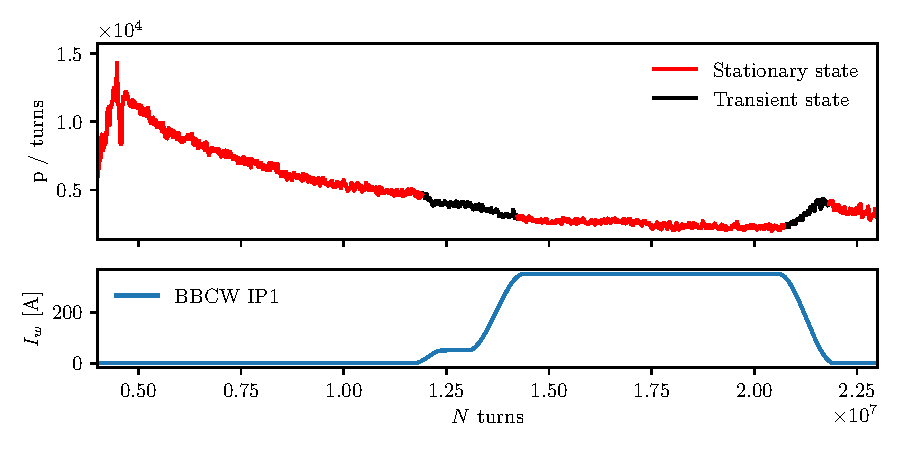
\includegraphics[width=1.0\textwidth]{5_wire_compensators_LHC/figs/stationary_transient.pdf}
    \caption{Visualization of the difference between stationary state and transient state for a slice of data. We define as stationary state the time interval in which all the parameters of the system are in a steady state, while the transient state is the time interval in which the system is undergoing a variation. Here, the BBCW DC current is switched on to the target voltage, causing a transient state along the process.}
    \label{fig:transient-state}
\end{figure}

In Fig.~\ref{fig:chunks}, we show the BLM data for Beam~1 and Beam~2 divided into enumerated chunks where the system is in the stationary state. We can see how the stationary states are generally longer than the transient states, except for the part where the octupoles change state.

\begin{figure}[hpt]
    \centering
    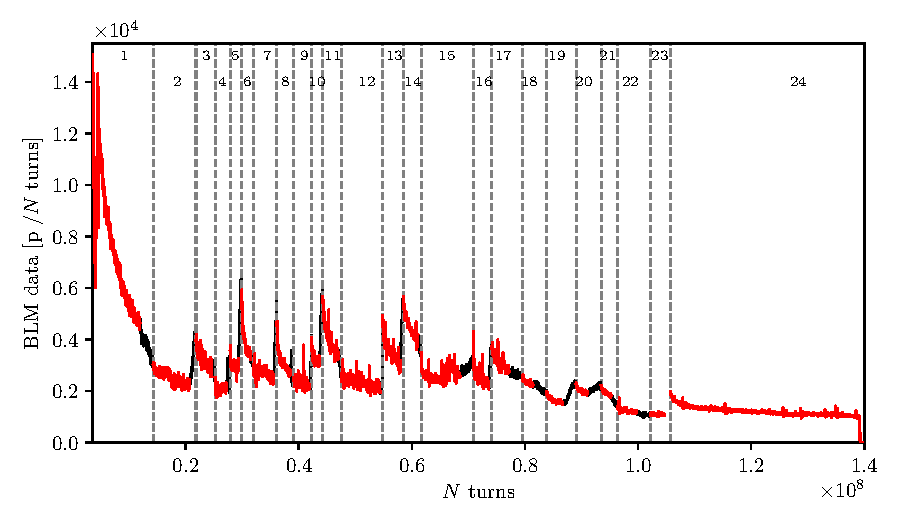
\includegraphics[width=1.0\textwidth]{5_wire_compensators_LHC/figs/chunks_names.pdf}
    \caption{Experimental data of Beam~2 divided in chunks, where each chunk is in a stationary state. Each chunk is characterized by a different set of parameters, and the system is in a transient state when the parameters are changed. Each chunk has a number assigned, which will be used to identify it for the rest of the analysis. Red corresponds to stationary state data, while black represents transient state data.}
    \label{fig:chunks}
\end{figure}

We assume that the beam distribution at the end of a stationary state can be used as the initial condition of the next stationary state. Therefore, we completely neglect the transient state losses between the two stationary states. To justify this approach, however, we must know that the integrated loss in the transient state must not be significantly comparable to the integrated loss in the stationary state.

In Fig.~\ref{fig:wire_loss_comp}, this comparison is shown for each individual chunk, and it is possible to see how the interval where the octupole state is changed has higher relative transient losses. Such comparable losses led us to the decision not to inspect this chunk of data characterized by varying octupoles, and we performed our fitting procedure only to the data up to those variations.

\begin{figure}[hpt]
    \centering
    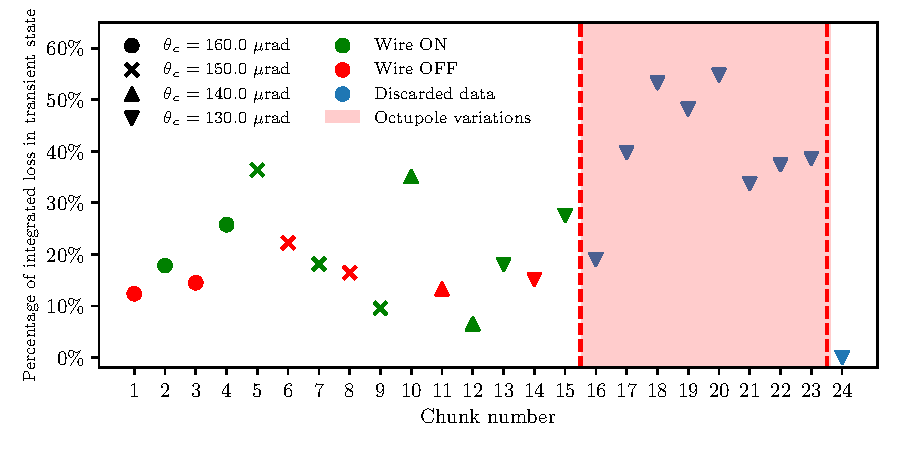
\includegraphics[width=1.0\textwidth]{5_wire_compensators_LHC/figs/losses_comparison.pdf}
    \caption{Comparison of the integrated losses in transient state and in stationary state for each chunk of data. The chunk numbers follow the nomenclature defined in Fig.~\ref{fig:chunks}. A higher relative loss in the transient states can be seen for the chunk where the octupoles are changed.}
    \label{fig:wire_loss_comp}
\end{figure}

Now that we have defined the data we will use for the fitting procedure, we can define the initial beam distribution we will use for the fitting. We consider a Gaussian beam distribution with unitary $\sigma$, which in action variables reads as a negative exponential distribution $\rho_0(I) = \exp(-I)$. To fit the data, we use the same procedure as in the work of Bazzani et al.~\cite{bazzani2020diffusion}, that is, we scan the values $\kappa$ and $I_\ast$, and integrate the evolution of the FP equation over the number of turns. The $\epsilon^2$ parameter is then fixed by requiring that the initial and final values of the relative intensity, evaluated at the beginning and at the end of the chunk, are equal.

As we assume that the beam distribution at the end of a stationary state can be used as the initial condition of the next stationary state, we can use the evolved beam distribution as the initial condition for the next chunk. This procedure, iterated for all chunks, finally gives us the reconstructed $D(I)$ for the various states of the system.

\section{Numerical results}

We performed the fitting procedure for the data of both Beam~1 and Beam~2. As the wires are installed on Beam~2 only, we do not expect to observe a significant difference between $D(I)$ reconstructed on the Beam~1 chunks with wire on and wire off. However, the data of Beam~1 is useful for both understanding the effects of different crossing angles on the system and establishing the characteristics of the results provided by the fitting procedure.

\subsection*{Beam~1 data}

We first consider the data of Beam~1 divided in chunks only where the crossing angle is varied. In Fig.~\ref{fig:reconstruction_1}, we show the relative intensity loss, along with the fit reconstruction. Note that we considered Beam~1 data up to the point at which the octupole current is varied. In Fig.~\ref{fig:reconstruction_2}, we show the reconstructed $D(I)$ for the various crossing angles.

We can see how $D(I)$ increases as the crossing angle is lowered, as expected from the fact that long-range beam-beam effects are more important, and we can also observe how in general the fitting procedure manages to reproduce the data quite well. %The evolution of the three parameters, $\epsilon$, $I_\ast$, and $\kappa$, is shown in Fig.~\ref{fig:parameters_1}. No significant patterns can be observed in the evolution of the parameters.%; however, the resulting $D(I)$ given by the three parameters increases as the crossing angle is lowered.

\begin{figure}[hpt]
    \centering
    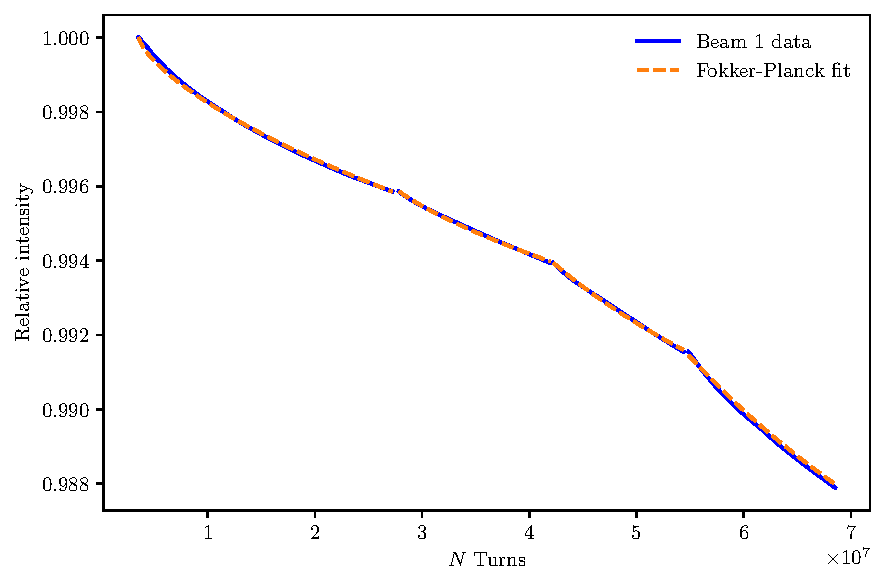
\includegraphics[width=1.0\textwidth]{5_wire_compensators_LHC/figs/losses_b1.pdf}
    \caption{Relative loss of intensity for the data of Beam~1 divided in chunks where the crossing angle is varied. The fit reconstruction is also shown. A good agreement between the data and the fit is observed.}
    \label{fig:reconstruction_1}
\end{figure}

\begin{figure}[hpt]
    \centering
    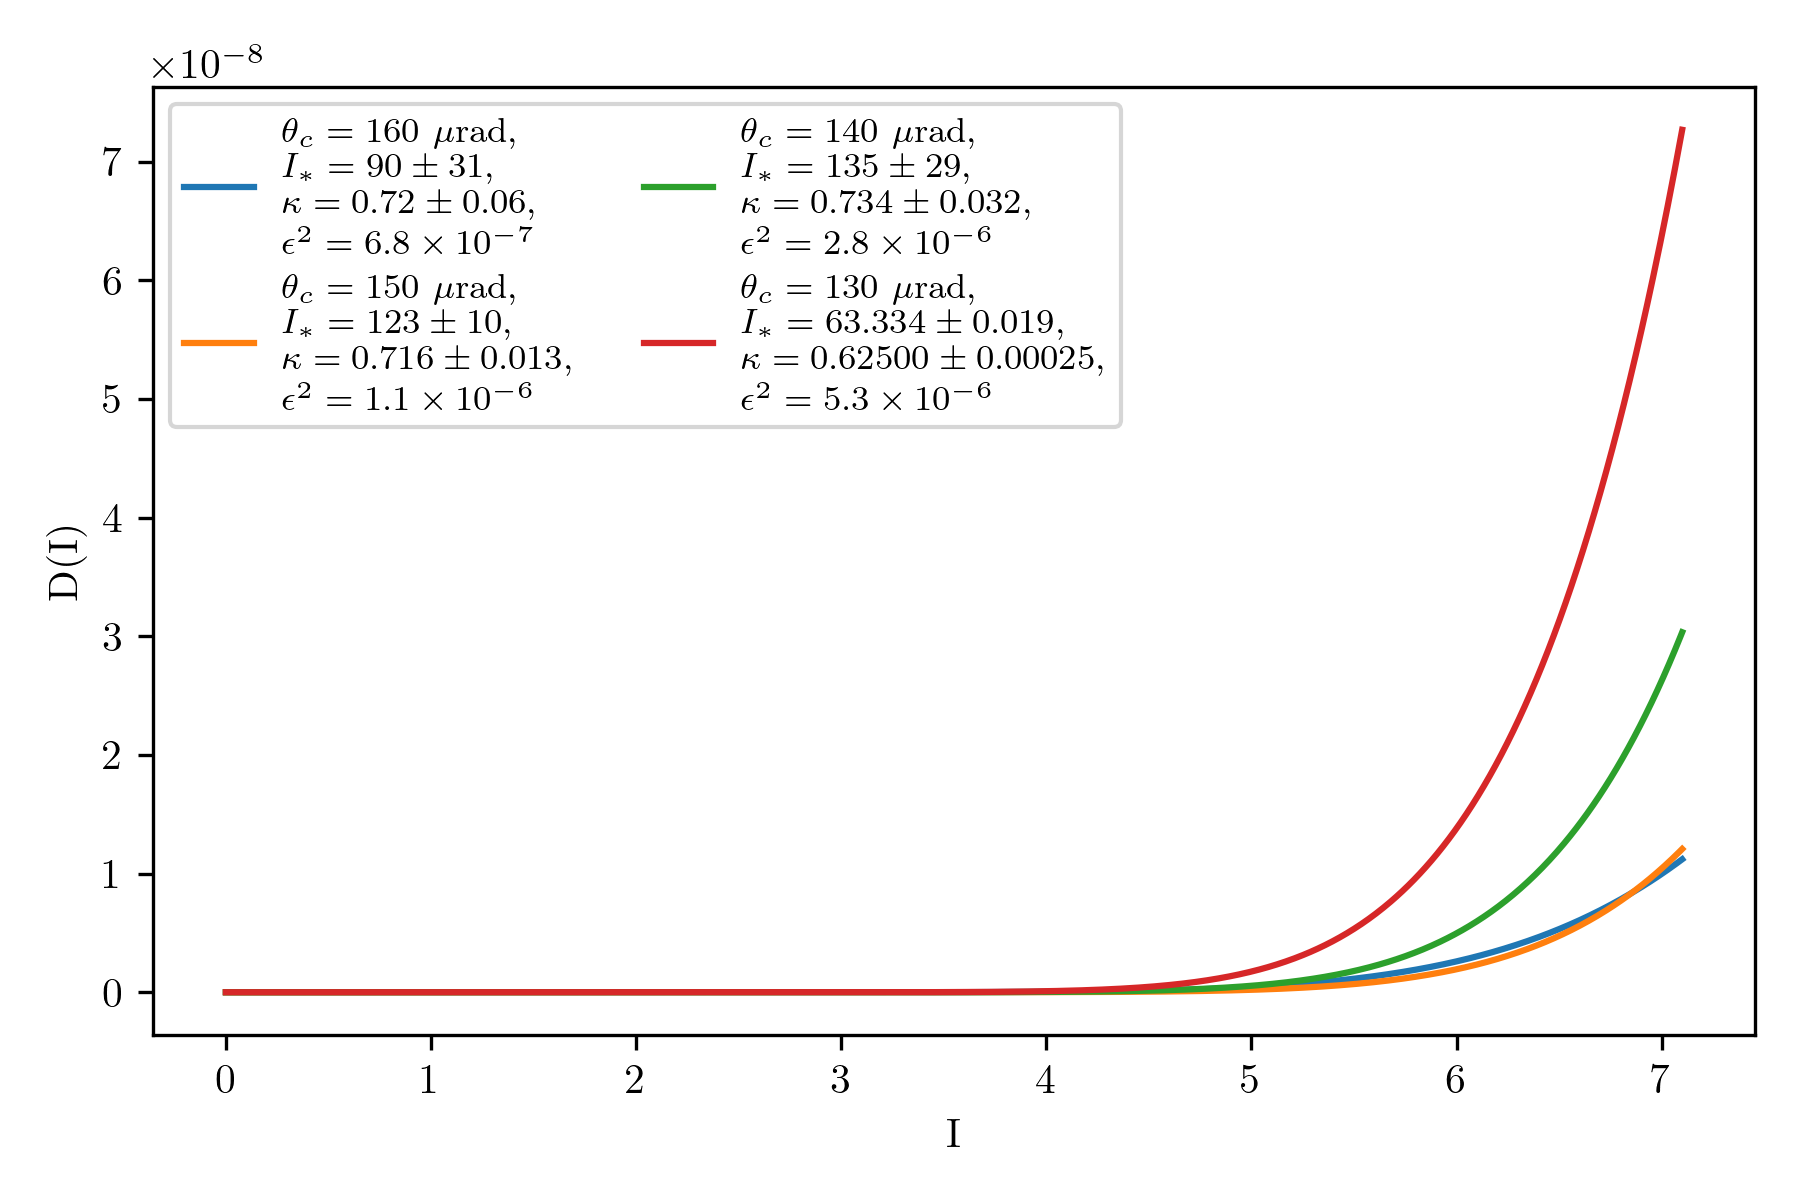
\includegraphics[width=1.0\textwidth]{5_wire_compensators_LHC/figs/fokker_planck_b1_D.png}
    \caption{Reconstructed $D(I)$ for the data of Beam~1 divided in chunks where the crossing angle is varied. The $D(I)$ increases as the crossing angle is lowered.}
    \label{fig:reconstruction_2}
\end{figure}

%\begin{figure}[hpt]
%    \centering
    % \includegraphics[]{}
%    \caption{Evolution of the three parameters, $\epsilon$, $I_\ast$, and $\kappa$, for the data of Beam~1 divided in chunks where the crossing angle is varied. No significant patterns can be observed in the evolution of the parameters.}
%    \label{fig:parameters_1}
%\end{figure}

If we instead consider the data of Beam~1 divided in chunks where the wire compensators are switched on and off, we can see how the $D(I)$ reconstructed, presented in Fig.~\ref{fig:reconstruction_3}, while manifesting differences, does not show a consistent different diffusion value between the two states. Moreover, extreme differences are also obtained from the $D(I)$ reconstructed from the full chunk also at lower $I$ values. This suggests that the fitting procedure might be affected by overfitting when the chunks are too small and not rich enough in information.

A comparison of the $\chi^2$ values of the fit for the two different chunking methods is shown in Fig.~\ref{fig:chi2}. We can see that the $\chi^2$ values are mostly lower when smaller chunks are considered, but not consistently. This suggests that, as no consistent differences can be observed in the reconstructed $D(I)$ between the wire-on and wire-off states, and as overfitting issues are observed at some fitting chunks, that, indeed, the BBCW on Beam~2 is not significantly affecting the beam dynamics on Beam~1.

\begin{figure}[hpt]
    \centering
    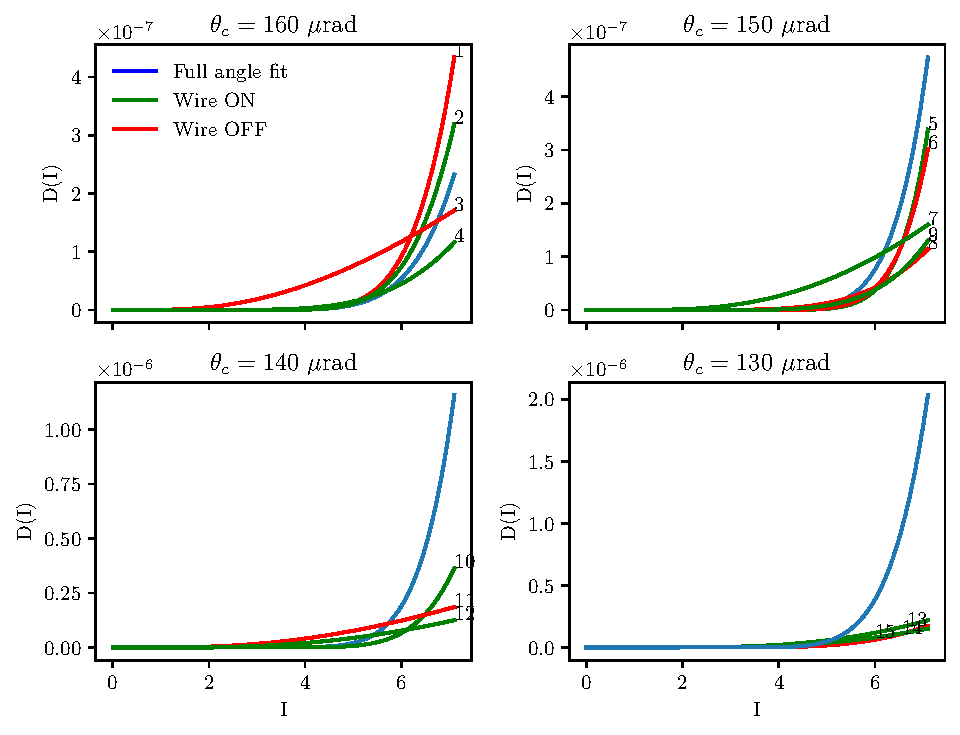
\includegraphics[width=1.0\textwidth]{5_wire_compensators_LHC/figs/fokker_planck_b1_turbo_bis.pdf}
    \caption{Reconstructed $D(I)$ for the data of Beam~1 divided in chunks where the wire compensators are switched on and off, compared with the $D(I)$ reconstructed using the full chunk corresponding to the crossing angle. The $D(I)$ does not show a consistent different diffusion value between the two states and, in multiple situations, the values obtained for $D(I)$ on the smaller samples obtain extremely different results from the full fitting result for low values of $I$. This suggests overfitting issues. The numbers follow the nomenclature in Fig.~\ref{fig:chunks}.}
    \label{fig:reconstruction_3}
\end{figure}

\begin{figure}[hpt]
    \centering
    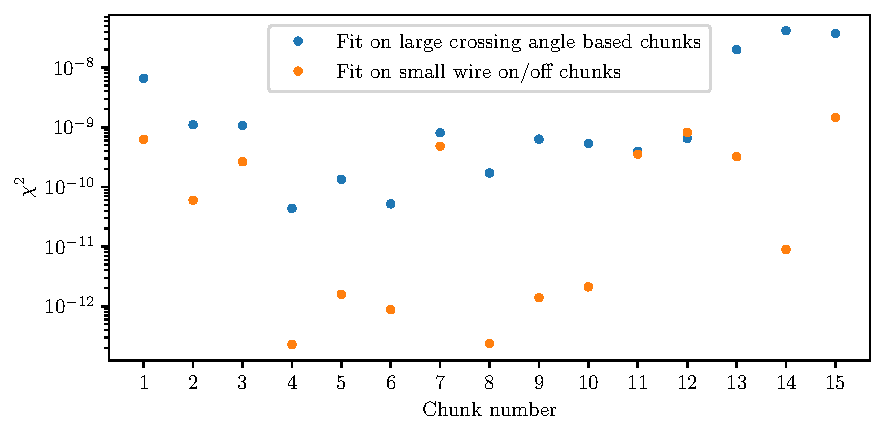
\includegraphics[width=1.0\textwidth]{5_wire_compensators_LHC/figs/chi2_b1.pdf}
    \caption{Comparison of the $\chi^2$ values of the fit for the two different chunking methods. The $\chi^2$ values are mostly lower when smaller chunks are considered, but not consistently so. The numbers follow the nomenclature in Fig.~\ref{fig:chunks}.}
    \label{fig:chi2}
\end{figure}

\subsection*{Beam~2 data}

We now inspect the data of Beam~2, where the wires are installed. We consider the data divided in chunks as presented in Fig.~\ref{fig:chunks}. In Fig.~\ref{fig:reconstruction_4}, we show the relative intensity loss, along with the fit reconstruction. In Fig.~\ref{fig:reconstruction_5}, we show the reconstructed $D(I)$ for the various crossing angles and the various wire states.

It can be seen that, in general, the fit reconstruction is able to reproduce the data quite well. Furthermore, it is possible to see how the reconstructed $D(I)$ is consistently different when the wires are switched on and off, with generally higher diffusion values when the wires are off. This is in agreement with the expectation that the wires are able to reduce the long-range beam-beam effects and thus the diffusion. Moreover, it is possible to see how such a reconstructed $D(I)$ for wire on states also has lower values for low $I$ amplitudes. This suggests that indeed the BBCWs might provide a better long-term stability of the beam.

The values of the two parameters, $I_\ast$ and $\kappa$, are shown in Fig.~\ref{fig:parameters_3}. Also in this case, no significant patterns can be observed in the evolution of the parameters for the different states of the system.

%To quantify the effects of the wires on the long-term beam dynamics, we can take the various reconstructed $D(I)$ for one of the crossing angles and consider the evolution of the relative intensity and emittance of a Gaussian distribution with a Fokker-Planck evolution over a number of turns of a higher order of magnitude. In Fig.~\ref{fig:evolution}, we show the evolution of the relative intensity and emittance for the various $D(I)$ reconstructed for the crossing angle of \SI{150}{\micro\radian}. We can see how the wires are able to archive a lower relative intensity. The emittance appear to decrease faster for cases where $D(I)$ is higher, this is due to the functional shape of $D(I)$ that, we recall, implies a semi-stationary distribution following Eq.~\eqref{}, which can be seen in Fig.~\ref{}. Such distribution describes a slow erosion that implies a reduction in emittance.

\begin{figure}[hpt]
    \centering
    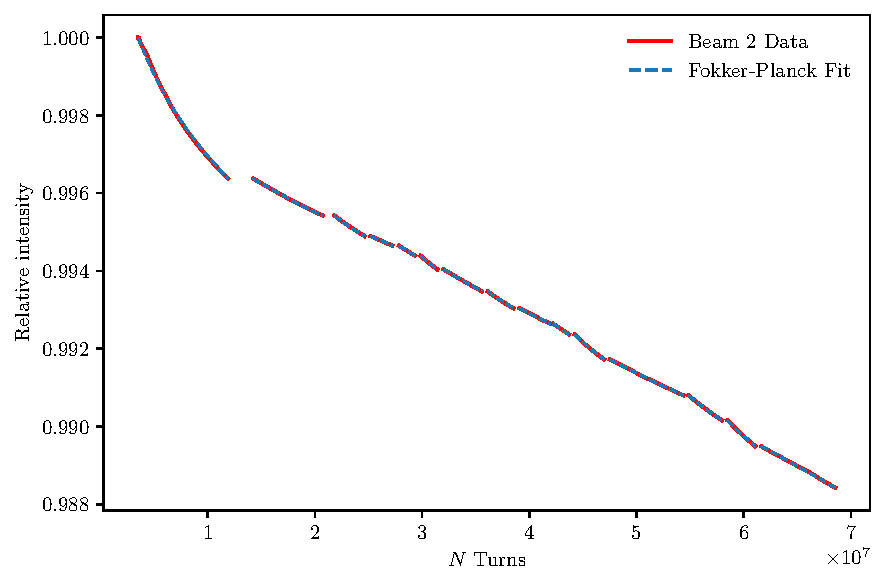
\includegraphics[width=1.0\textwidth]{5_wire_compensators_LHC/figs/losses_b2.pdf}
    \caption{Relative intensity loss and fit reconstruction for the data of Beam~2 divided in chunks, following the nomenclature of Fig.~\ref{fig:chunks}. 
    The fit reconstruction is able to reproduce the data quite well.}
    \label{fig:reconstruction_4}
\end{figure}

\begin{figure}[hpt]
    \centering
    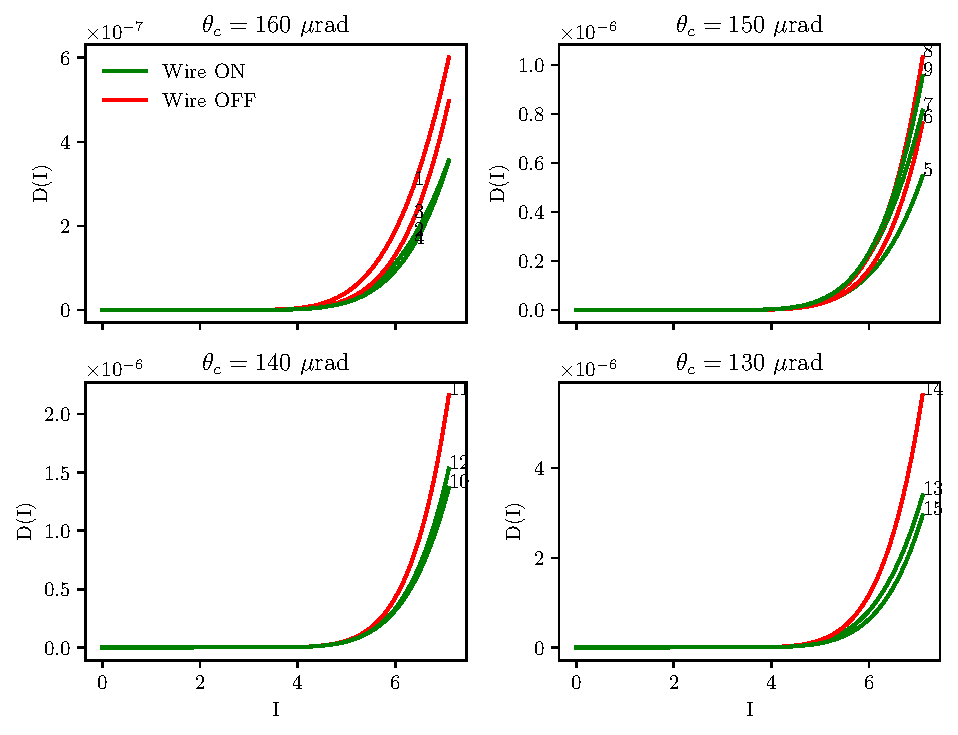
\includegraphics[width=1.0\textwidth]{5_wire_compensators_LHC/figs/fokker_planck_b2_2.pdf}
    \caption{Reconstructed $D(I)$ for the data of Beam~2 divided in chunks, following the nomenclature of Fig.~\ref{fig:chunks}. It can be seen how the reconstructed $D(I)$ is consistently different when the wires are switched on and off, with in general higher diffusion values when the wires are off. The only exception is given by chunk 6, with a crossing angle of $\theta_c=$\SI{150}{\micro\radian}.}
    \label{fig:reconstruction_5}
\end{figure}

\begin{figure}[hpt]
    \centering
    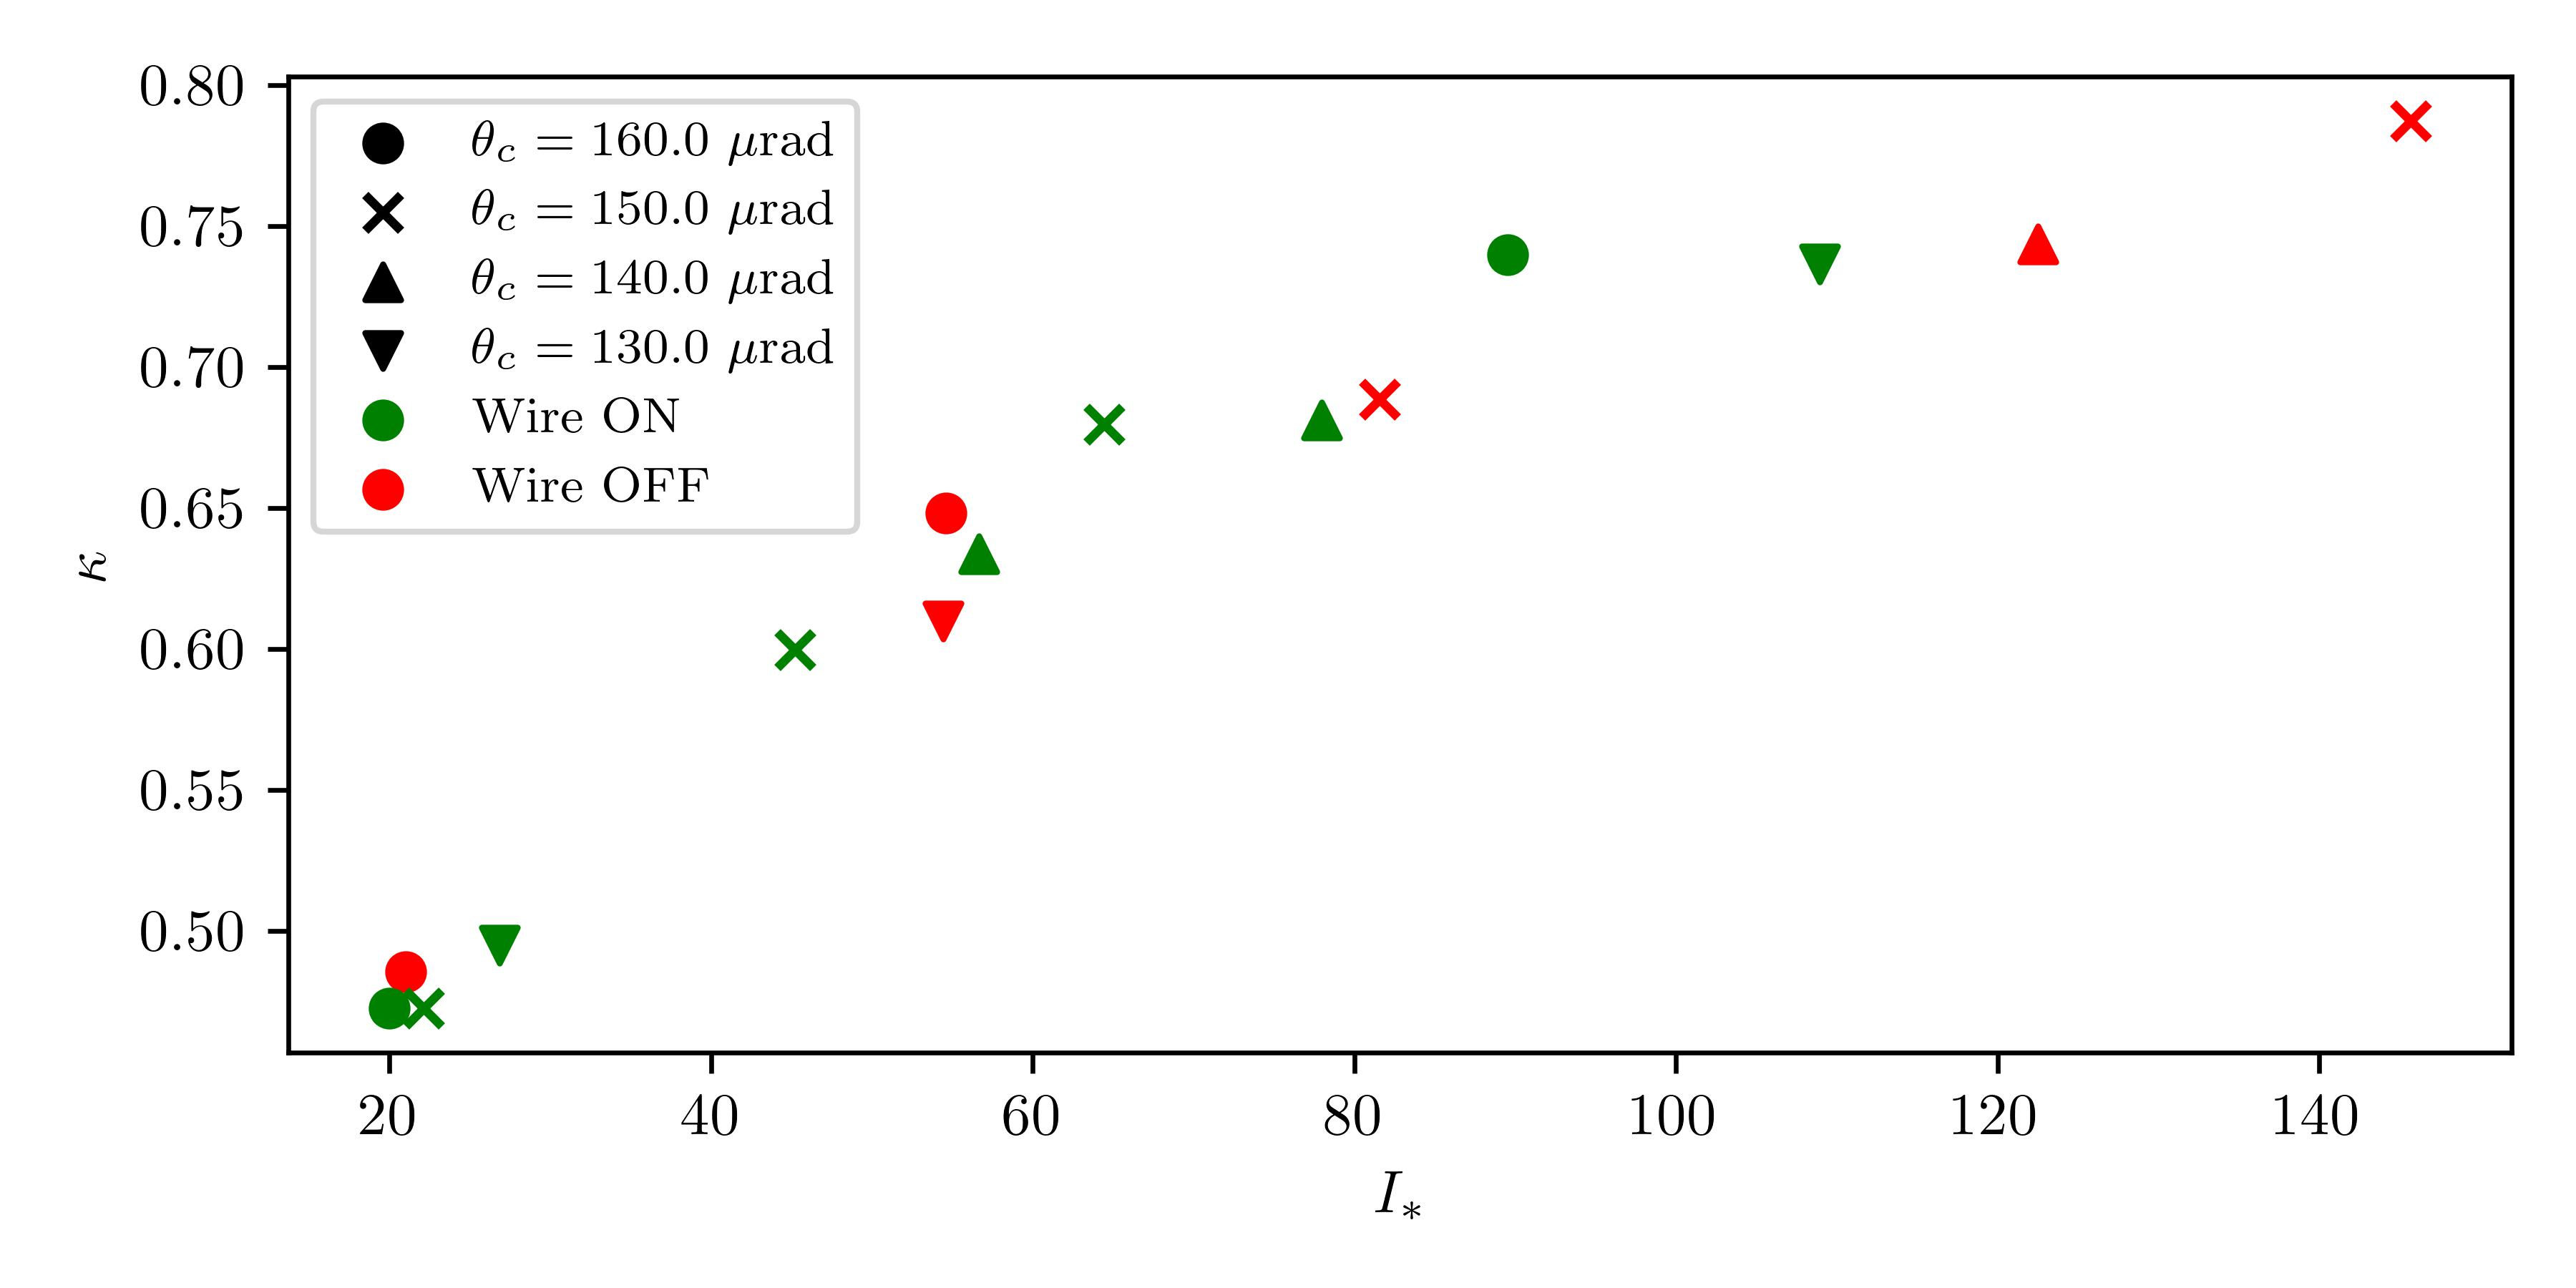
\includegraphics[width=1.0\textwidth]{5_wire_compensators_LHC/figs/fokker_planck_b2.jpg}
    \caption{Evolution of the parameters $I_\ast$, and $\kappa$, for the data of Beam~2 divided in chunks, following the nomenclature of Fig.~\ref{fig:chunks}. No significant patterns can be observed in the evolution of the parameters.}
    \label{fig:parameters_3}
\end{figure}

%\begin{figure}[hpt]
%    \centering
%    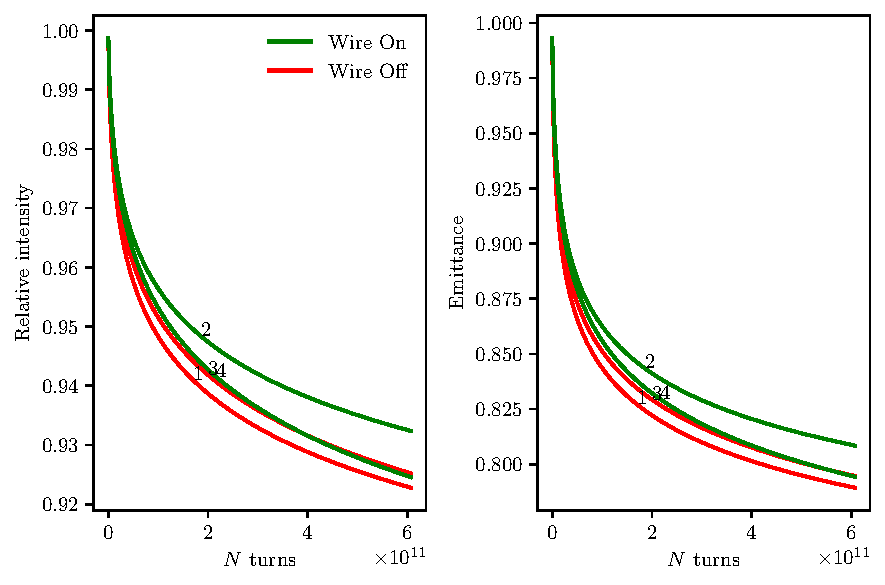
\includegraphics[width=1.0\textwidth]{5_wire_compensators_LHC/figs/sim_emittance.pdf}
%    \caption{Evolution of the relative intensity and emittance for the various $D(I)$ reconstructed for the crossing angle of \SI{160}{\micro\radian}. The evolution is obtained by simulating a Fokker-Planck process, with a Gaussian distribution as initial condition. A lower $D(I)$ yields lower relative losses and lower emittance decrease.}
%    \label{fig:evolution}
%\end{figure}

\section{Final remarks}

We have performed an initial study of the effects of the BBCWs on the long-term beam dynamics of the LHC using our diffusive framework. We have used the data of the LHC Beam~1 and Beam~2, taken during an MD measurement campaign of Run2, and we have reconstructed the $D(I)$ of various system configurations. Ultimately, we have found that the wires are able to reduce the long-range beam-beam effects and thus the diffusion. Moreover, we have observed that our model suggests that the wires are consistently able to archive a lower intensity loss. As expected, the model did not highlight significant BBCWs effects on Beam~1.

As pointed out in the overview of the experimental data, a large portion of the data had to be discarded because of the large amount of losses occurring during transient periods. Moreover, multiple chunks considered in the analysis are characterized by a very short time span, which might be too short to be representative of the long-term beam dynamics. This is a limitation of the data that might have had a significant impact on the results.

However, the promising results obtained in the fit reconstruction seem to suggest that this diffusive framework can provide some insight into the long-term effects of BBCWs on beam dynamics. This has motivated us to consider a different data gathering strategy for the scheduled MD measurements of LHC Run3. More specifically, we planned to measure the BLM losses while keeping the BBCWs on and off for longer time spans, in order to better characterize the long-term effects of the wires.

Additionally, we planned to perform collimation scans with BBCWs on and off, in order to directly inspect the beam tail population and measure $D(I)$ following the protocol presented in Chapter~\ref{ch:probing}. The purpose was to compare the values obtained with the two different methodologies.

Both of these strategies in the data gathering have been successfully implemented during the MD measurement campaign of LHC Run3~\cite{}, and the results will be presented in a future work.

\part{Dynamic indicators for detecting regular and chaotic motion}\label{part:dyn}

\chapter{Overview of dynamic indicators}\label{ch:overview_of_dynamic_indicators}
\noindent\textsf{The content of this chapter, with the due adaptations, has resulted in the article by A.\ Bazzani, M.\ Giovannozzi, C.\ E.\ Montanari, G.\ Turchetti \textit{``Performance analysis of indicators of chaos for non-linear dynamical systems''}, currently under internal peer review.}

\vspace{3em}

After investigating the applicability of a Nekhoroshev-like diffusive models to the study of beam loss data, we now switch our focus to the topic of single-particle tracking and, consequently, to the problem of characterising the long-term dynamics of non-linear symplectic maps, which of course includes realistic accelerator one-turn maps.

In this chapter, we focus on the identification of chaotic behaviour in the orbits of complex dynamical systems by using dynamic indicators. Dynamic indicators have been already proposed, and new ones have been designed with the goal of enhancing the detection of chaos in numerical simulations. The difficulty lies in forecasting chaotic behaviour by analysing orbits of a restricted length. To inspect the properties of these indicators, and assess which ones are the best performing, we carry out an accurate analysis of the performance of the indicators briefly introduced to classify the orbits of a 4\textsc{d} modulated polynomial symplectic map, namely a 4\textsc{d} H\'enon map that is considered a reference model for several applications. 

The chapter is structured as follows. In Section~\ref{sec:dyn:intro}, we give a brief introduction on the topic of chaos indicators, as well as a summary of the dynamic indicators under analysis; in Section~\ref{sec:dyn:review} we define mathematically and discuss in some detail the chaos indicators considered; in Section~\ref{sec:dyn:numerical_implementations} we discuss their numerical implementation; in Section~\ref{sec:dyn:results} we present the numerical results and rank the different indicators in terms of classification efficiency, in particular, studying their predictive power. Finally, some conclusions are drawn in Section~\ref{sec:dyn:conc}. In addition, we report some detail on the computational cost of implementing indicators using parallel computing facilities in Appendix~\ref{app:computing}, while some considerations on the time dependence of indicators are presented in Appendix~\ref{app:timedep}. 

\section{\label{sec:dyn:intro}Introduction}
%
The study of the long-term evolution of Hamiltonian systems is a very difficult task from both a theoretical and a numerical point of view. The KAM theory~\cite{KAM4} cannot be used to solve the stability problem for Hamiltonian systems in more than two dimensions. Therefore, great effort has been devoted to improving time stability estimates after the celebrated Nekhoroshev theorem~\cite{Nekhoroshev:1977aa}. However, the existence of chaotic layers in phase space strongly affects the long-term evolution of the orbits, and for this reason, numerical indicators have been proposed to detect the chaotic character of orbits using a limited number of time iterations. 

For a given Hamiltonian model, one has to tackle the problem of comparing the performance of the various indicators to assess which one provides the optimal classification of the orbits. In applications, this task must be accomplished taking into account the characteristics of the physical problem under consideration. For instance, in the field of accelerator physics, the study of the charged-hadron motion in the magnetic lattice of a circular accelerator is often devoted to the determination of the region of phase space in which bounded motion occurs. The extent of such a region is called dynamic aperture and involves studying the stability of orbits of a 6D polynomial symplectic map in a neighbourhood of an elliptic fixed point, up to $10^8-10^9$ iterations~(see, e.g.,~\cite{Bazzani:262179}). An exhaustive analysis of the phase-space topology is clearly beyond the current computational capabilities. Therefore, indicators of chaos turn out to be extremely useful to reduce the amount of computational time needed to assess the character of orbits (regular or chaotic). This task may be affected by the presence of orbit diffusion in phase space, which occurs in chaotic layers. The presence of small stochastic effects, which naturally arise in physical systems, may prevent orbit trapping near regular regions, the so-called stickiness phenomenon~\cite{Kandrup1999DiffusionAS,SZEZECH2005394}, thus inducing diffusive behaviour in phase space. 

It is worth noting that polynomial symplectic maps are not only central for the analysis of accelerator physics problems, as they are also present in other domains and have been intensively studied to understand the phase space structure of Hamiltonian systems~\cite{Turaev2003}, and are a fundamental tool for long-term integration of orbits~\cite{Bazzani:262179}. 

The main result of this chapter is to show that it is possible to determine a classification performance ranking of the main commonly used chaotic indicators when applied to a generic 4\textsc{d} cubic polynomial symplectic map of H\'enon-like form (see, e.g., ~\cite{Bazzani:262179}), which is an excellent prototype dynamical system for applications.

The indicators of chaos are typically based on the existence of positive Lyapunov characteristic exponents, and their numerical performance is strongly affected in the regions where sticky orbits are present.

The family of Fast Lyapunov indicators ($FLI$)~\cite{Froeschle1997} has been proposed to distinguish the regions of regular and chaotic motion for symplectic maps~\cite{SZEZECH2005394}. They also proved to be suitable for distinguishing resonant regions in phase space and to visualise the Arnold web of resonances where slow diffusion occurs~\cite{Arnold:937549}. These indicators are based on the evolution of an initial deviation vector and provide the linear response of the tangent map along an orbit. When considering one or more initial deviation vectors, the result depends on the direction of the initial deviation vectors. To overcome this, the linear response to a random displacement vector with zero mean value and unit variance was recently proposed~\cite{Turchetti2017}. The trace of the corresponding covariance matrix defines the square Lyapunov Error ($LE$), which is similar to $FLI$. Furthermore, the invariants of the covariance matrix of order $k>1$ are asymptotically related to the sum of the first $k$ Lyapunov exponents. However, unlike the Generalized Alignment Index ($GALI^{(k)}$) indicators~\cite{Bountis2007,Skokos2015}, these invariants do not depend on the initial deviations~\cite{Skokos2008}. Recently, a couple of approaches have been proposed to improve the performance of some indicators, namely applying the Weighted Birkhoff averaging~\cite{Das_2017} or the Mean Exponential Growth of Nearby Orbit ($MEGNO$)~\cite{Cincotta1996}, which is used to filter the oscillations and to improve the accuracy by averaging on map iterations~\cite{Gozdziewski01,Mestre2011}.

To calculate the sensitivity to small deviations along an orbit, the Reversibility Error Method ($REM$) can be used~\cite{Panichi2016,Panichi2017}. In this case, the linear response to the forward evolution in the presence of small random noise is considered, followed by the unperturbed backward evolution. The covariance matrix of the random process, which provides the final deviation from the initial condition in the limit of zero noise amplitude, can be computed, and its invariants quantify the violation of reversibility. The first invariant for the forward-backward process $BF$ is the square of the reversibility error, which is equal to the sum of the squares of Lyapunov errors computed at each iteration of the map. This invariant can be compared with the results for $REM$, when the stochastic perturbation is generated by the finite numerical precision present in both the forward and backward directions. 

Finally, a completely different indicator introduced by J.Laskar~\cite{Laskar1999,Laskar2003} is represented by the Frequency Map Analysis $FMA$, which computes the variation of the main frequency of a given orbit considering different orbit lengths to detect the chaotic character. 
%
\section{Definition and main properties of indicators of chaos} \label{sec:dyn:review}
%
\subsection{Frequency Map Analysis\label{subsec:dyn:fma}}
%
Originally introduced by J.~Laskar in the field of celestial mechanics, the Frequency Map Analysis ($FMA$) rapidly expanded outside the initial domain of application (see, e.g., \cite{laskar1995frequency,lega1996numerical,papaphilippou1996frequency,papaphilippou1998global,Laskar1999, Papaphilippou1999, laskar2000application,PhysRevSTAB.4.124201,1288929,Papaphilippou:PAC03-RPPG007,Laskar2003,PhysRevSTAB.6.114801,shun2009nonlinear,PhysRevSTAB.14.014001,papaphilippou2014,tydecks:ipac18-mopmf057,PhysRevAccelBeams.22.071002} for a selected list of references, with special emphasis on accelerator-related applications) is a numerical method to inspect the global dynamics of multidimensional Hamiltonian systems, taking advantage of the quasiperiodicity of regular orbits located on KAM tori.

Given a Hamiltonian system $H(I,\theta) = H_0 (I) + \varepsilon H_1 (I, \theta)$, where for $\varepsilon=0$ the Hamiltonian $H_0(I)$ is integrable and $(I, \theta$ are action angle variables in $\mathbb{R}^n \times \mathbb{T}^n$, where $\mathbb{T}$ represents a one-dimensional torus. %with equations of motion given for $j=1,\ldots,n$:
%\begin{equation}
%    \dot{I_j}=0,\quad \dot{\theta_j} = \frac{\partial %H_0(I)}{\partial I_j} = \nu_j(I).
%\end{equation}
If the system is nondegenerate,
\begin{equation}
    \operatorname{det}\left(\frac{\partial \nu(I)}{\partial I}\right)=\operatorname{det}\left(\frac{\partial^2 H_0(I)}{\partial I^2}\right) \neq 0 \,,
\end{equation}
the application
\begin{equation}
    \begin{array}{r}
    F: I\in \mathbb{R}^{n} \longrightarrow \nu\in \mathbb{R}^n 
    \end{array}
\end{equation}
is a diffeomorphism on its image. This means that the invariant tori are equally identified by the action variables $I$ or by their corresponding frequency vector $\mathbf{\nu}$. For a nondegenerate system, when $\varepsilon$ is sufficiently small, the KAM theorem~\cite{KAM1,KAM2,KAM3}, states that there still exists a set of initial conditions of positive measure that correspond to regular orbits on invariant tori, for which, according to Pöschel~\cite{Poschel1982}, a similar diffeomorphism still applies.

Based on this theoretical framework, it is possible to distinguish between regular orbits on the KAM tori, which feature a discrete structure for Fourier components defined by the harmonic of the fundamental frequencies, and chaotic orbits, which exhibit a complex structure in the Fourier spectrum~\cite{1288929}. In this sense, $FMA$ is a technique that performs numerical evaluations of the frequency vector $\vb{\nu}$ from a time series corresponding to a certain interval $[i, i+n]$, for different values of $i$. In case of a regular orbit lying on a KAM tori, the frequency vectors for various $i$ will agree up to the precision of the numerical method used to determine the frequency. On the other hand, a chaotic orbit will have $\vb{\nu}$ that evolves over different intervals, showing fluctuations in frequency space~\cite{laskar2000application}.

To achieve an accurate numerical evaluation of fundamental frequencies, multiple studies have been carried out to improve standard algorithms such as the Fast Fourier Transform (FFT) or the Average Phase Advance (APA)~\cite{laskar1992measure,Laskar1999, Bartolini:316949,bartolini1998computer}. In the work of Bartolini et al.~\cite{Bartolini:292773}, the fundamental frequency is evaluated using an FFT combined with a Hanning filter and an interpolation algorithm, resulting in a closed-form formula for the fundamental frequency. In recent studies~\cite{russo:ipac2021-thpab189}, the frequency determination carried out using the average phase advance algorithm is improved by applying the weighted Birkhoff averaging~\cite{Das_2018}, which will be used in the sequel to perform the evaluation of $FMA$.
More precisely, we define $FMA_n$ as the Euclidean distance between two vectors defined by the fundamental frequencies $\nu_1$ and $\nu_2$, evaluated respectively over the time intervals $[0, n/2]$ and $[n/2, n]$ of the orbit. An initial condition on a KAM torus has $FMA_n$ converge to zero when $n\to \infty$. In contrast, an initial condition in a chaotic layer will converge to an asymptotic value for $FMA_n$ bounded away from zero.
%
\subsection{Lyapunov Error invariants\label{subsec:dyn:le}}
%
Let $M(\xbf,n)$ be a time-dependent symplectic map with $\xbf\in \mathbb{R}^{2d}$ where the first $d$ components of $\xbf$ are the space coordinates and the last $d$  their conjugate moments. Denoting by $DM$ the Jacobian matrix $(DM)_{ij}=\partial M_i/\partial x_j$ and by $\xbf_n$ the orbit after $n$ iterations, the corresponding tangent map $\Lop_n(\xbf)$ is defined by 
%
\begin{equation}
  \begin{aligned}
  &\xbf_n =M(\xbf_{n-1},n-1) \equiv M_n(\xbf) \,,   &\xbf_0=\xbf;& \\ \\
  &\Lop_n(\xbf) = DM(\xbf_{n-1}, n-1) \,\Lop_{n-1}(\xbf)  \equiv DM_n(\xbf) \,,     &\Lop_0=\Iop \, , &
  \end{aligned}
  \label{eq2-1}
\end{equation}
%
where $M_n(\xbf)= M(\xbf,n-1)\circ M_{n-1}(\xbf)$ with $M_0(\xbf)=\xbf$.

For any initial condition $\xbf$, consider a small stochastic deviation $\eps\boldsymbol{\xi}$ where
$\boldsymbol{\xi}$ is a unit random vector with $\mean{\boldsymbol{\xi}}=0$ and a unit covariance matrix $\mean{\boldsymbol{\xi}\,\boldsymbol{\xi}^T}=\Iop $, where the suffix $^T$ denotes the transposed vector. Letting $\ybf_n=M(\ybf_{n-1},n-1)$ be the orbit with initial condition $\ybf_0=\xbf_0+\eps\boldsymbol{\xi}$ the linear response $\boldsymbol{\Xi}_n(\xbf)$, initialised by $\boldsymbol{\Xi}_0=0$ is given by 
%
\begin{equation}
  \begin{split}
    \boldsymbol{\Xi}_n (\xbf) &= \lim_{\eps \to 0}\,\frac{\ybf_n-\xbf_n}{ \eps} \\
    %\lim_{\eps \to 0}\,{M(\ybf_{n-1},n-1) - M(\xbf_{n-1},n-1) \over \eps}=
     &= DM(\xbf_{n-1},n-1)\,  \times   \lim_{\eps \to 0} \frac{\ybf_{n-1}-\xbf_{n-1}}{ \eps} \\
     &= DM(\xbf_{n-1},\,n-1)  \boldsymbol{\Xi}_{n-1} \\
     &= \Lop_n(\xbf)\,\boldsymbol{\xi} \,.
  \end{split}
  \label{eq2-2}
\end{equation}
%
The random vector $\boldsymbol{\Xi}_n$ has zero mean and covariance matrix
%
\begin{equation}
    \Sigma^2_n(\xbf)= \mean{\boldsymbol{\Xi}_n(\xbf)\boldsymbol{\Xi}_n^T(\xbf)}= \Lop_n(\xbf)\Lop_n^T(\xbf) \,.
    \label{eq2-3}
\end{equation}
%
Oseledet theorem~\cite{Oseledets1961} states that the limit
\begin{equation}
    \lim_{n\to\infty}(\Lop_n^T\Lop_n)^{1/2n}= \Wop\,e^{\Lambda}\,\Wop^T 
\end{equation}
exists, where $\Wop$ is an orthogonal symplectic matrix and $\Lambda$ is diagonal with entries $\lambda_j(\xbf)$ ordered in a decreasing sequence in $j$.

The diagonal entries of $\Lambda$ are the Lyapunov exponents, and the columns of $\Wop$ the corresponding Lyapunov vectors. Since the eigenvalues of $\Lop_n^T\Lop_n$ are the same as those of the covariance matrix $\Lop_n\Lop_n^T$, the two matrices have the same characteristic polynomial. Then consider the corresponding invariants $I_n^{(k)}(\xbf), k=1,\ldots,2d$, i.e., the coefficients of the characteristic polynomial. The first invariant $I^{(1)}_n(\xbf)$, is given by the trace of the covariance matrix, namely,
%
\begin{equation}
  I^{(1)}_n(\xbf)\equiv \Tr\bigl(\Sigma^2_n(\xbf)\bigr)= \Tr\bigl(\Lop_n^T(\xbf)\,\Lop_n(\xbf)\bigr)=LE_n^2(\xbf) \,,
   \label{eq2-5}
\end{equation}
%
which is the square of the Lyapunov error $LE_n(\xbf)$. Note that it does not depend on the initial deviation vector or on the chosen orthogonal reference frame, and its asymptotic behaviour is determined by the first, i.e., largest, Lyapunov exponent $\lambda_1$.

The other invariants $I^{(k)}$ are the sum of all products that combine $k$ distinct eigenvalues if they are simple. The geometric interpretation is straightforward. Letting $\ebf_j$ be the standard base vectors, we have $\Lop_n=(\ebf_{1\,\,n},\ldots,\ebf_{2d\,\,n})$where $\ebf_{j\,\,n}=\Lop_n\,\ebf_j$. %  is   the image of the base vector $j$  by the tangent map.
As a consequence, the invariant $I_n^{(k)}(\xbf)$ is the sum of the squared volumes of the $\genfrac(){0pt}{2}{2d}{k}$ parallelotopes whose sides are the vectors $\ebf_{j_1\,\,n}(\xbf),\ldots,\ebf_{j_k\,\,n}(\xbf)$.

The difference with respect to $GALI^{\,(k)}_{\,n}$ indicators (see Section~\ref{subsec:dyn:other}), is that the $I^{(k)}_n(\xbf)$ are  independent of the initial displacements. 

For a symplectic map, $\Lop_n(\xbf)$ is a symplectic matrix, and $\Sigma^2_n(\xbf)=\Lop_n(\xbf)\,\Lop_n^T(\xbf)$ is symplectic and positive definite. As a consequence, ordering the eigenvalues in a decreasing sequence, we have $e^{\lambda_{j;n}}e^{\lambda_{2d-j+1;n}}=1$. The asymptotic behaviour of the invariant $I_n^{(k)}, k\le 2d$ is given by 
%
\begin{equation}
  \lim_{n\to \infty}\,\frac{1}{2n}\,\log I^{(k)}_n(\xbf) = \lambda_1(\xbf)+\ldots+\lambda_k(\xbf) \, .
  \label{eq2-7}
\end{equation}
%

In a region of chaotic motion, $\lambda_{j\,\,n}(\xbf)$ are positive for $j\le d$ just as their limit $\lambda_j(\xbf)$,  so that $I_n^{(k)}(\xbf)$ has exponential growth with $n$, for $n$ sufficiently large. In a region of regular motion, $I^{(k)}_n(\xbf)$ grows according to a power law $I^{(k)}_n(\xbf) \sim n^{2k}$ for $k\le d$ as all Lyapunov exponents vanish.
%
\subsection{Fast Lyapunov Indicator and Weighted Birkhoff averaging\label{subsec:dyn:fli}}
%
The Fast Lyapunov Indicator~\cite{Froeschle1997}, is one of the best known dynamic indicators, due to its straightforward implementation and its sensitiveness to the detection of chaotic structures~\cite{Lega2016fli}. Given $M(\vb{x}, n)$, its tangent map $\Lop_n(\xbf)$, and an arbitrary initial unitary deviation vector $\boldsymbol{\xi}$, $FLI$ is defined for $n\geq1$, as:
\begin{equation}
    FLI_n(\vb{x}_0, \boldsymbol{\xi}) = \ln{\norm{\Lop_n(\xbf_0) \boldsymbol{\xi}}} \, ,
    \label{eq:fli}
\end{equation}
i.e., the logarithm of the linear response $\boldsymbol{\Xi}_n(\xbf)$, calculated for an arbitrary fixed deviation vector. The quantity $FLI_n/n$ tends to the largest Lyapunov exponent as $n\to \infty$. Therefore, in a region of regular motion, this quantity tends to zero, whereas in a region of chaotic motion it takes a positive value.

It is possible to take advantage of the properties of the logarithm in Eq.~\eqref{eq:fli} to avoid overflows for large values of $n$, and to express the limit $FLI_n/n$ as an average along the trajectory $\xbf_n$~\cite{Alligood1996}:
%
\begin{equation}
\begin{aligned}
    \frac{FLI_n(\vb{x}_0, \boldsymbol{\xi})}{n} &= \sum_{i=0}^{n-1} \frac{\ln{\norm{\vb{y}_i-\vb{x}_i}}}{n},\\ 
    \vb{y}_i &= DM(\vb{x}_{i-1}, i-1)\frac{\vb{y}_{i-1}-\vb{x}_{i-1}}{\norm{\vb{y}_{i-1}-\vb{x}_{i-1}}} \,,\\
    \vb{y}_1 &= DM(\vb{x}_0, 0)\boldsymbol{\xi}\,.
    \label{eq:fli_mean}
\end{aligned}
\end{equation}
%
In the work of Das et al.~\cite{Das_2017}, it is presented how the application of the Weighted Birkhoff averaging method $\mathrm{WB}_n$~\cite{Das_2018} in the evaluation of $FLI$ can lead to superconvergence properties when applied to oscillating time series. Instead of considering equal weighting $(1/n)$, the Weighted Birkhoff averaging method uses a weighting function $w\left(\frac{i}{n}\right)$, which acts similarly to a window function in spectral analysis. A function $w(t)$ that proved to be very effective in improving the convergence of quasiperiodic time series averages~\cite{Das_2018} reads as follows:
%
\begin{equation}
    w(t):= 
    \begin{cases}
        \exp \left[-\frac{1}{t(1-t)}\right], & \text { for } t \in(0,1) \\ 
        0, & \text { for } t \notin(0,1)
    \end{cases} \,.
    \label{eq:birkhoff}
\end{equation}
%
Replacing the standard mean with $w(t)$ in Eq.~\eqref{eq:fli_mean} leads to the weighted Fast Lyapunov Indicator $FLI_n^{WB}$:
%
\begin{equation}
    FLI_n^{WB}(\vb{x}_0, \boldsymbol{\xi}) = \sum_{i=0}^{n-1} w\left(\frac{i}{n}\right) \ln{\norm{\vb{y}_i}} \, .
    \label{eq:fli_birkhoff}
\end{equation}
%
We expect that $FLI_n^{WB}(\vb{x}_0, \boldsymbol{\xi})$ converges faster than $FLI_n(\vb{x}_0, \boldsymbol{\xi})/n$ to their common limit in the case of regular orbits, at least.

To simplify the notation, in the numerical analysis we refer to $FLI_n(\vb{x}_0, \boldsymbol{\xi})/n$ and $FLI_n^{WB}(\vb{x}_0, \boldsymbol{\xi})$ as $FLI_n(\boldsymbol{\xi})/n$ and $FLI_n^{WB}(\boldsymbol{\xi})$, respectively, specifying the choice made for the initial unitary displacement $\boldsymbol{\xi}$. 
%
\subsection{Backward-Forward reversibility error\label{subsection:bf}}
%
The reversibility error is obtained by computing the linear response of the dynamics to small additive stochastic perturbations on the orbit after $n$ forward iterations $n$ followed by $n$ backward iterations 
%
\begin{equation}
 \begin{split}
   &\ybf_{n'}  = M(\ybf_{n'-1},n'-1) +\eps\boldsymbol{\xi}_{n'} \, ,  \quad \ybf_0=\xbf \, , \quad 1\le n'\le n \, ; \\ 
   &\ybf_{n'} = M^{-1}(\ybf_{ n'-1}, 2n-n')+\eps   \boldsymbol{\xi}_{n' } \, , \quad n+1\le n'\le 2n \, .
  \end{split}
\label{eq2-8}
\end{equation}
%
where $\boldsymbol{\xi}_{n'}$ are random vectors with zero mean and unit covariance matrix $\langle\boldsymbol{\xi}_{n'}\rangle=0$  and $\langle\boldsymbol{\xi}_{n'} \boldsymbol{\xi}_{n''}^T\rangle=\delta_{n' n''}$.
%Using the numerical finite precision as additive noise is a natural choice, but one can use an additional noise. Random displacement in backward iterations can be chosen equal to zero by setting
$\boldsymbol{\xi}_{n'}=0$ for $n'>n$. We denote by $\xbf_{n'}$ the orbit when random deviations are absent $\eps=0$. This orbit
enjoys the symmetry property $\xbf_{n'}= \xbf_{2n-n'}$ for $n+1\le n'\le 2n$, so the reversibility condition $\xbf_{2n}=\xbf$ is satisfied.

The linear response for the $BF$ process is defined by 
%
\begin{equation}
 %\begin{split}
   \boldsymbol{\Xi}^{BF}_{n'}(\xbf)  = \lim_{\eps\to 0}\frac{\ybf_{n'}-\xbf_{n'}}{ \eps},  \quad \qquad  1\le n'\le 2n,  %\\ \\
%   \boldsymbol{\Xi}^{BF}_{n'}(\xbf)   &= \lim_{\eps\to 0}{\ybf_{n'}-\xbf_{2n-n'}\over \eps}   \qquad n\le n'\le 2n \\ \\ 
  %\end{split}
\label{eq2-9}
\end{equation}  
%
and the cumulative random deviation $\boldsymbol{\Xi}^{BF}_{n'}(\xbf)$satisfies the recurrence 
%
\begin{equation}
  \begin{aligned}
  & \boldsymbol{\Xi}_{n'}^{BF} = DM(\xbf_{n'-1},n'-1)\,\boldsymbol{\Xi}_{n'-1}^{BF}(\xbf)+ \boldsymbol{\xi}_{n'} \, , \quad 1\le n'\le n;\\ 
    & \boldsymbol{\Xi}_{n'}^{BF} = DM^{-1}(\xbf_{2n-n' +1},2n-n')\, \boldsymbol{\Xi}_{n'-1}^{BF}    + \boldsymbol{\xi}_{n'} \, , \quad n+1 \le n'\le 2n \, .
  \end{aligned}
\label{eq2-10}
\end{equation}
%

From the recurrence relation of the tangent map~\eqref{eq2-1} evaluated for $n'$ and from the equality $DM^{-1}(M(\xbf,k),k))\,DM(\xbf,k)=\Iop$ for $k=2n-n'$ it follows 
%
\begin{equation}
  \begin{split}
  DM(\xbf_{n'-1},\,n'-1) &= \Lop_{n'}(\xbf)\,\Lop_{n'-1}^{-1}(\xbf) \, , \\
  DM^{-1}(\xbf_{2n-n' +1},2n-n') &= \Bigl(DM(\xbf_{2n-n'},2n-n')\,\Bigr)^{-1} \\
  &= \Lop_{2n-n'}(\xbf)\,\Lop^{-1}_{2n-n'+1}(\xbf) \, .
  \end{split}
\label{eq2-11}
\end{equation}
%
Replacing Eq.~\eqref{eq2-11} in Eq.~\eqref{eq2-8} we obtain the final result
%
\begin{equation}
    \begin{split}
      \boldsymbol{\Xi}_{n}^{BF}(\xbf) & = \,\Lop_n(\xbf)\,\sum_{k=1}^n\,\Lop_k^{-1}(\xbf) \,\boldsymbol{\xi}_k \,; \\  
       \boldsymbol{\Xi}_{2n}^{BF}(\xbf) &= \Lop_n^{-1}(\xbf)\,\boldsymbol{\Xi}_{n}^{BF}(\xbf)+ \sum_{k=0}^{n-1}\,\Lop^{-1}_k(\xbf)\,
      \boldsymbol{\xi}_{2n-k} \\ % = \\
      &  =\sum_{k=1}^{n-1}\,\Lop_k^{-1}(\xbf)\,(\boldsymbol{\xi}_k+\boldsymbol{\xi}_{2n-k}) \,+
     \,\boldsymbol{\xi}_{2n}+ \Lop_n^{-1}(\xbf) \boldsymbol{\xi}_n .
     \end{split}
  \label{eq2-12}
  \end{equation}
%
If random deviations are present only in the forward process, the covariance matrix of $\boldsymbol{\Xi}^{BF}_{2n}$ is given by 
%
\begin{equation}
    \Sigma^{2\,\,BF}_n(\xbf) = \parmean{  \boldsymbol{\Xi}^{BF}_{2n}(\xbf)\bigl(\boldsymbol{\Xi}^{BF}_{2n}(\xbf)\bigr)^T} =\sum_{k=1}^n \,\bigl( \,\Lop_k^T(\xbf)\Lop_k(\xbf)\,\bigr)^{-1}\, .
\label{eq2-13}
\end{equation}
%
If random deviations are present both in the forward and backward processes, we define $\Sigma^{2\,\,BF}_n$ as $1/2$ the covariance matrix of $\boldsymbol{\Xi}^{BF}_{2n}$, and the result is the r.h.s. of Eq.~\eqref{eq2-13} where the last term of the sum $(\Lop_n^T\Lop_n)^{-1}$ is replaced by $\frac{1}{2}\, \Iop+\frac{1}{2} (\Lop_n^T\Lop_n)^{-1}$ due to the boundary condition, and asymptotically, for $n\to \infty$ the difference is negligible. 
\begin{comment}
Finally, to get another indicator, one can reverse the previous process by considering first the backward evolution defined by the map $M^{-1}(\xbf,-k)$  followed by the $F$ evolution (see the Appendix for more details). 
\end{comment}

The invariants of the matrix $\Sigma^{2\,\,BF}_n$ provide
information on the effect of small random perturbations along the orbits. If the map $M$ is symplectic, both $\Lop_n$ and $\Lop_n^T\Lop_n$ are symplectic matrices and the trace of$\Lop_n^T\Lop_n$ and its inverse are equal. As a consequence, it is not difficult to check that the trace of $\Bigl(\sum_{n'}\,\bigl(\Lop_{n'}^T\,\Lop_{n'}\bigr)^{-1}\,\Bigr)^k$ and of $\Bigl(\sum_{n'}\, \Lop_{n'}^T\,\Lop_{n'}\,\Bigr)^k$ are equal and the invariants of the covariance matrices of the $BF$ process become
%
\begin{equation}
   I^{(k)\,\,BF}_n(\xbf)= I^{(k)} \parton{\sum_{k'=1}^n\,\Bigl(\Lop_{n'}^T(\xbf)\,\Lop_{n'}(\xbf)\,\Bigr)^{-1}} =I^{(k)} \parton{\sum_{k'=1}^n\,\Lop_{n'}^T(\xbf)\,\Lop_{n'}(\xbf)\,} \, .
%    I^{(k)\,\,FB}_n(\xbf)& = I^{(k)} \parton{\sum_{k'=1}^n\,\Bigl(\Lop_{-n'}^T(\xbf)\,\Lop_{-n'}(\xbf)\,\Bigr)^{-1}} \\% = \\
%  & =  I^{(k)} \parton{\sum_{k'=1}^n\,\Lop_{-n'}^T(\xbf)\,\Lop_{-n'}(\xbf)\,} .
\label{eq2_18}
\end{equation}
%

The first invariant has a very simple relation to the Lyapunov error $LE_n(\xbf)$. Explicitly, we have the following.
%
\begin{equation}
   \Bigl(E^{BF}_n (\xbf))\Bigr)^2  \equiv I^{(1)\,\,BF}_n(\xbf) = \sum_{n'=1}^n \,\Tr \Bigl(\Lop^T_{n'}(\xbf)
   \Lop_{n'}(\xbf) \Bigr) =  \sum_{n'=1}^n \,  \Bigl(LE_n (\xbf))\Bigr)^2 \,. 
%   \Bigl(E^{FB}_n (\xbf))\Bigr)^2 \equiv I^{(1)\,\,FB}_n(\xbf) &= \sum_{n'=1}^n \,\Tr \Bigl(\Lop^T_{-n'}(\xbf)
%  \Lop_{-n'}(\xbf) \Bigr) \\
%   &=  \sum_{n'=1}^n \,  \Bigl(LE_{-n} (\xbf))\Bigr)^2 \,.
\label{eq2_19}
\end{equation}
%
\begin{comment}
For an integrable map with $d=1$, given by  $M(\xbf)= \Rop(\Omega)\xbf$  with
$\Omega=\Omega(\frac{1}{ 2}  \xbf\cdot \xbf)$
one has $\Tr(\Lop_n^T\Lop_n)= 2 +\left( \xbf\cdot\xbf\,\,\Omega'\,\,n\right)^2$ and in this case
$LE_{-n}=LE_n$ and $E^{BF}_n =LE_{-n}$. For a generic orbit of a non-integrable system,
$LE_n$ and $LE_{-n}$ differ, although asymptotically the difference is usually negligible. 

Adding a weak dissipation, the fixed and periodic elliptic points become attractive, and the Lyapunov errors
$LE_n$ and $LE_{-n}$ and the $FB$ and $BF$ reversibility errors are substantially different,
and this is also the case for higher-order invariants.
\end{comment}

We conclude by observing that the $BF$ reversibility error analysis can be applied to investigate the effect of rounding errors in numerical computations~\cite{PANICHI201653}. Letting $M_\eps$ be the map evaluated with roundoff errors and $M_\eps^{-1}$ its inverse, we have $M^{-1}_\eps(M_\eps(\xbf))= \xbf+ O(\eps)$. In the IEEE 754 international standard, the precision of a real number is $\eps\sim 10^{-16}$. Iteration with rounding is defined by Eq.~\eqref{eq2-8} where $\eps\xi_{n'}$ is missing, but $M$ is replaced by $M_\eps$. The matrix $\frac{1}{ 2}\, \boldsymbol{\Xi}_{2n}^{BF}\,\bigl(\boldsymbol{\Xi}_{2n}^{BF}\bigr)^T$, whose average defines the covariance matrix of the $BF$ reversibility error, is replaced by 
%
\begin{equation}
  \Xop_{2n}^{BF}(\xbf)= \frac{1}{ 2}\,\frac{ \ybf_{2n}-\xbf}{ \eps}\,\frac{(\ybf_{2n}-\xbf)^T}{\,\eps} \,.
\label{eq2_20}
\end{equation}  
%
This matrix has a non-zero eigenvalue, with eigenvector $\ybf_{2n}-\xbf$, and a null eigenvalue of multiplicity $2d-1$ with eigenspace orthogonal to $\ybf_{2n}-\xbf$. The noise-induced Reversibility Error Method ($REM$) squared is the non-zero eigenvalue of such a matrix, equal to is trace and given by  
%
\begin{equation}
    \Bigl(REM_n^{BF}(\xbf)\Bigr)^2 = \Tr\Bigl(   \Xop_{2n}^{BF}(\xbf)\Bigr) = \frac{1}{ 2} \,\, \frac{\ybf_{2n}-\xbf}{ \eps} \cdot \frac{\ybf_{2n}-\xbf}{ \eps} \,.
\label{eq2_21}
\end{equation}
%
%  which is the analogue of ${1\over 2}\, \boldsymbol{\Xi}\cdot\boldsymbol{\Xi}$ before taking the average, which leads to
%   $\bigl(E_{n}^{BF}(\xbf)\bigr)$.

The main difference is that $REM$, due to rounding, is the result of a single realization with a pseudorandom error and, therefore, is affected by large fluctuations when we vary $n$ or $\xbf$. These fluctuations are absent for the $BF$ reversibility error previously defined, since averaging over the random deviations is carried out. The other relevant difference is that the higher-order $REM$ invariants are zero.
\begin{comment}
We can define the indicator $REM$ for the FB process in the same way starting from the recurrence~\eqref{eq2-14} where $\boldsymbol{\xi}_{n'}$ is set to 0 and $M$ is replaced by $M_\eps$. The corresponding error is denoted by $REM_n^{FB}(\xbf)$.   %The major difference between $E^{BF}_n(\xbf)$ and
  % $REM_n^{BF}(\xbf)$ is that the first one is the result of an averaging process over the random
  % deviations whereas the second is the result of a  unique realization of a pseudo-random process.
In this case, $REM_n^{FB}(\xbf)$ is also close to $E^{FB}_n(\xbf)$ if fluctuations are washed out, for example, with a moving average in $n$. 
\end{comment}

Note that the implementation of $REM$ is trivial since it does not require the evaluation of the tangent map and the computational cost is just twice the cost of the orbit computation, provided that the inverse map is explicitly known. %This method has been used successfully in celestial mechanics. 
%
\subsection{$GALI^{(k)}$ indicators\label{subsec:dyn:other}}
%
  %Among the variational indicators  the fast Lyapunov indicator  was  first introduced by Froechelet et al.,
  %being  defined as
  %$FLI_{\,n}=\log \Vert\Lop_n(\xbf)\etabf\Vert$,  where $\etabf$ is a given unit vector.
  %The advantage of $E_n$ with respect to $FLI_{\,n}$ is its independence from the initial vector.
  %\\
The $k$-order indicators $GALI^{(k)}$ use the volumes of parallelotopes whose sides are normalized images of the $k$ linearly independent vectors $\boldsymbol{\eta}_j$ with $1\le j\le k$.
%
%\begin{equation}
%  \hskip -.2 truecm 
%  GALI^{(k)}_n ( \xbf)= \Vert \etabf_{1\,\,n}(\xbf)\wedge \cdots \wedge \etabf_{k\,\,n}(\xbf) \Vert
%  \quad \etabf_{j\,\,n }(\xbf)= {\Lop_n(\xbf) \etabf_j \over \Vert \Lop_n(\xbf) \etabf_j \Vert}
%  \label{eq2_22}
%\end{equation}
%
\begin{equation}
  GALI^{(k)}_n ( \xbf)= \left \Vert \frac{\Lop_n(\xbf) \boldsymbol{\eta}_1 }{ \Vert \Lop_n(\xbf) \boldsymbol{\eta}_1 \Vert}
    \wedge \ldots \wedge \frac{\Lop_n(\xbf) \boldsymbol{\eta}_k}{ \Vert \Lop_n(\xbf) \boldsymbol{\eta}_k\Vert} \right \Vert \,,
  \label{eq2_22}
\end{equation}
%
where $\wedge$ stands for the external product of two vectors. Their asymptotic behaviour for chaotic orbits, whose first $d$ Lyapunov exponents are positive, is given by
\begin{equation}
    GALI^{(k)}_n \sim e^{-n\,\bigl((\lambda_1-\lambda_2) +\ldots+(\lambda_1-\lambda_k)\,\bigr)}  \,.
\end{equation}
where we assume a decreasing order for the exponents.

For regular, quasi-periodic  orbits,  whose Lyapunov exponents vanish, the $GALI^{(k)}$ indicators decay following a power law. We recall that the Lyapunov error invariants $I_n^{(k)}$ grow exponentially with a coefficient given by the sum of the first $k$ Lyapunov exponents for chaotic orbits, or according to a power law for regular orbits. %Growth, rather than decay with $n$, is the first significant difference with the indicators $GALI^{(k)}$. The second significant difference between the indicators $LE$ and $RE$ with respect to $GALI^{(k)}$ is their invariance with respect to the choice of the initial deviation vectors.
\begin{comment}
Regarding the indicators of reversibility error, the origin in the 
literature can be found in~\cite{} with respect to rounding. We first introduce the reversibility error as the linear response to additive noise~\cite{} to provide a plausible justification for the reversibility breakdown due to rounding. For Hamiltonian systems, the reversibility error is simply related to the Lyapunov error according to the following intuitive result.
\begin{equation}
    \bigl(\,E^{BF}_n(\xbf)\,\bigr)^2 =LE^2_1(\xbf) + LE^2_2(\xbf) +\ldots+LE^2_n(\xbf)\,.
\end{equation}
\end{comment}
%
\subsection{Introducing filters}
%
We conclude by remarking that the introduction of a filter such as $MEGNO$ that drastically reduces the numerical oscillations of the indicator of chaos~\cite{Gozdziewski01, Cincotta2016}, may greatly improve the efficiency of the indicator. In principle, the oscillations disappear using suitable normal coordinates for the considered systems, but their computations face the limits and technical difficulties of perturbation theory. Referring to the phase flow that interpolates the orbits at integer times $t=n$, $MEGNO$, applied to $LE_t(\vb{x})$, it has the double-time average of $d\log LE_t(\vb{x})/d\log t$  %= 2t\,d \log E(t)/dt$   
%
\begin{equation}
\begin{split}
    MEGNO_n(LE(\vb{x})) & =  %\mean{\mean{  {d\log E^2(t)\over d\log t} }}= 
   \left\langle\left\langle  t\, \frac{d\log LE_t(\vb{x})}{ dt}\right \rangle \right \rangle\, \\
 \text{where} \qquad \mean{f(t)}& = \frac{1}{ t}\,\int_0^t \,f(t')\,dt' \, .
\end{split}
\label{eq3-23}
\end{equation}
%
If the indicator $LE_n(\vb{x})$ grows exponentially as $e^{\lambda t}$, then $MEGNO_n(LE(\vb{x}))$ increases as $\lambda t$. If $LE_n(\vb{x})$ follows the power law $t^\alpha$, then $MEGNO_n(LE(\vb{x}))$ converges to $2\alpha$.%, while it converges to $(2\alpha+1)/2$ for $E^{BF}(\vb{x})$.

%When $LE_n$ has exponential growth, $\mathrm{d}/\mathrm{d}n \log LE_n$ can converge to $\lambda$ more rapidly than $t^{-1}\,\log LE_n$ and faster convergence to $\lambda$ is expected for $(2t)^{-1}\,MEGNO_n(LE)$.
%
\section{\label{sec:dyn:numerical_implementations} Numerical implementations}
%
\subsection{Models}
%
To test the effectiveness of the proposed indicators of chaos, we consider a 4\textsc{d} polynomial symplectic map dependent on time, which is a generalisation of the Hénon map~\cite{Bazzani:262179}. The origin is an elliptic fixed point, and the non-linear terms combine fixed quadratic non-linearities and variable cubic ones. The map reads:
%\begin{widetext}
\begin{equation}
    \left(\begin{array}{c}
    x_{n+1} \\
    p_{x, n+1} \\
    y_{n+1} \\
    p_{y, n+1}
    \end{array}\right) =R(\omega_{x,n}, \omega_{y, n}) \left(\begin{array}{c}
    x_{n} \\
    p_{x, n}+x_{n}^{2}-y_{n}^{2} + \mu \left(x_{n}^{3} - 3x_{n}y_{n}^{3}\right) \\
    y_{n} \\
    p_{y, n}-2 x_{n} y_{n} + \mu \left(y_{n}^{3} - 3y_{n} x_{n}^{3}\right)
    \end{array}\right) \,,
    \label{eq:henon}
\end{equation}
%\end{widetext}
where $\mu$ represents the intensity of the cubic non-linearity and $R$ is a $4\times 4$ rotation matrix defined as
\begin{equation}
    R(\omega_{x,n}, \omega_{y, n})=\left(\begin{array}{cc}
    R\left(\omega_{x, n}\right) & 0 \\
    0 & R\left(\omega_{y, n}\right)
    \end{array}\right) \,,
\end{equation}
with $R\left(\omega_{x, n}\right)$ and $R\left(\omega_{y, n}\right)$ being $2\times 2$ rotation matrices. In the sequel, we refer to the map~\eqref{eq:henon} as the 4\textsc{d} Hénon map and remark that it is often used as a reference model in applications such as accelerator physics (see, e.g., \cite{Bazzani:262179, invlog, Bazzani:2019csk}), since it represents the dynamics generated by a magnetic lattice that includes sextupole and octupole magnets~\cite{Bazzani:262179}.

Linear frequencies $\omega_{x, n}$ and $\omega_{y, n}$ are slowly modulated as a function of time $n$ according to
\begin{equation}
    \begin{aligned}
    &\omega_{x, n}=\omega_{x, 0}\left(1+\varepsilon \sum_{k=1}^{m} \varepsilon_{k} \cos \left(\Omega_{k} n\right)\right) \,, \\
    &\omega_{y, n}=\omega_{y, 0}\left(1+\varepsilon \sum_{k=1}^{m} \varepsilon_{k} \cos \left(\Omega_{k} n\right)\right) \,,
    \end{aligned}
\end{equation}
where $\varepsilon$ represents the modulation amplitude and the parameters $\varepsilon_k$ and $\Omega_k$ are taken from Table~1 in~\cite{invlog} to model the effect of frequency modulation in a particle accelerator due to ripples in the currents of the power supplies that feed the magnets. Modulation of the linear frequency may cause the appearance of weak chaotic regions in the stability basin near the origin. 
We recall that the parameters $\varepsilon_k$ have an order of magnitude of $10^{-4}$.

%These modulation parameters correspond to the tune modulation due to the observed ripple in the quadrupoles of the SPS~\cite{}. 
In numerical simulations, two sets of frequencies $\omega_{x0}$ and $\omega_{y0}$ have been considered, namely $(0.168,\ 0.201)$, which is close to resonances of order $5$ and $6$, and $(0.28,\ 0.31)$, which are the frequencies in the transverse phase space for charged particles orbiting in the LHC at injection energy.
We have analysed the performance of chaos indicators as a function of the parameters $\varepsilon$ and $\mu$, which have been varied in the intervals $[0,64]$ and $[0,1]$, respectively. Some considerations on the computational costs of implementing the various indicators of chaos in a parallel computing architecture are reported in the Appendix~\ref{app:computing}. 

%\begin{table}[h]
%    \centering
%    \begin{tabular}{lcc}
%        \toprule
%        $k$ & $\Omega_k$ & $10^4 \epsilon_k$ \\
%        \midrule
%        1 & $2\pi/868.12$ & 1.000 \\
%        2 & $2\Omega_1$   & 0.218 \\
%        3 & $3\Omega_1$   & 0.708 \\
%        4 & $6\Omega_1$   & 0.254 \\
%        5 & $7\Omega_1$   & 0.100 \\
%        6 & $10\Omega_1$  & 0.078 \\
%        7 & $12\Omega_1$  & 0.218 \\
%        \bottomrule
%    \end{tabular}
%    \caption{Modulation parameters for the Hénon map.}
%    \label{tab:modulation} 
%\end{table}

Figure~\ref{fig:survival} shows some survival plots for various configurations of the 4\textsc{d} Hénon map. A set of $300\times300$ initial conditions, sampled on a uniform Cartesian grid in the $x-y$ plane, choosing $p_x = p_y = 0$, is tracked up to $n_\mathrm{max}=10^8$ turns. Grid boundaries are selected to sample a region of interest that contains the stability basin of the origin, more specifically $[0.0,\,0.45]$ for case $(\omega_{x0},\,\omega_{y0}) = (0.168,\,0.201)$, or $[0.0,\,0.60]$ for case $(\omega_{x0},\,\omega_{y0}) = (0.28,\,0.31)$. An initial condition is considered stable if its distance from the origin is less than a certain control radius $r_\mathrm{c}$ when $n=n_\mathrm{max}$. Otherwise, the initial condition is considered lost and its tracking is stopped, and the stability time is given by the first value $n_\mathrm{stab}$ for which $\sqrt{x^2_{n_\mathrm{stab}}+ p_{x,n_\mathrm{stab}}^2+y_{n_\mathrm{stab}}^2+p_{y,n_\mathrm{stab}}^2}\geq r_\mathrm{c}$. The choice of $r_\mathrm{c}$ is rather arbitrary (we have considered $r_\mathrm{c}=10^2$) and the dependence of the results on $r_\mathrm{c}$ is very weak since at that amplitude the dynamics of the 4\textsc{d} Hénon map is fully dominated by polynomial terms. 
%
\begin{figure*}[th]
    \centering
    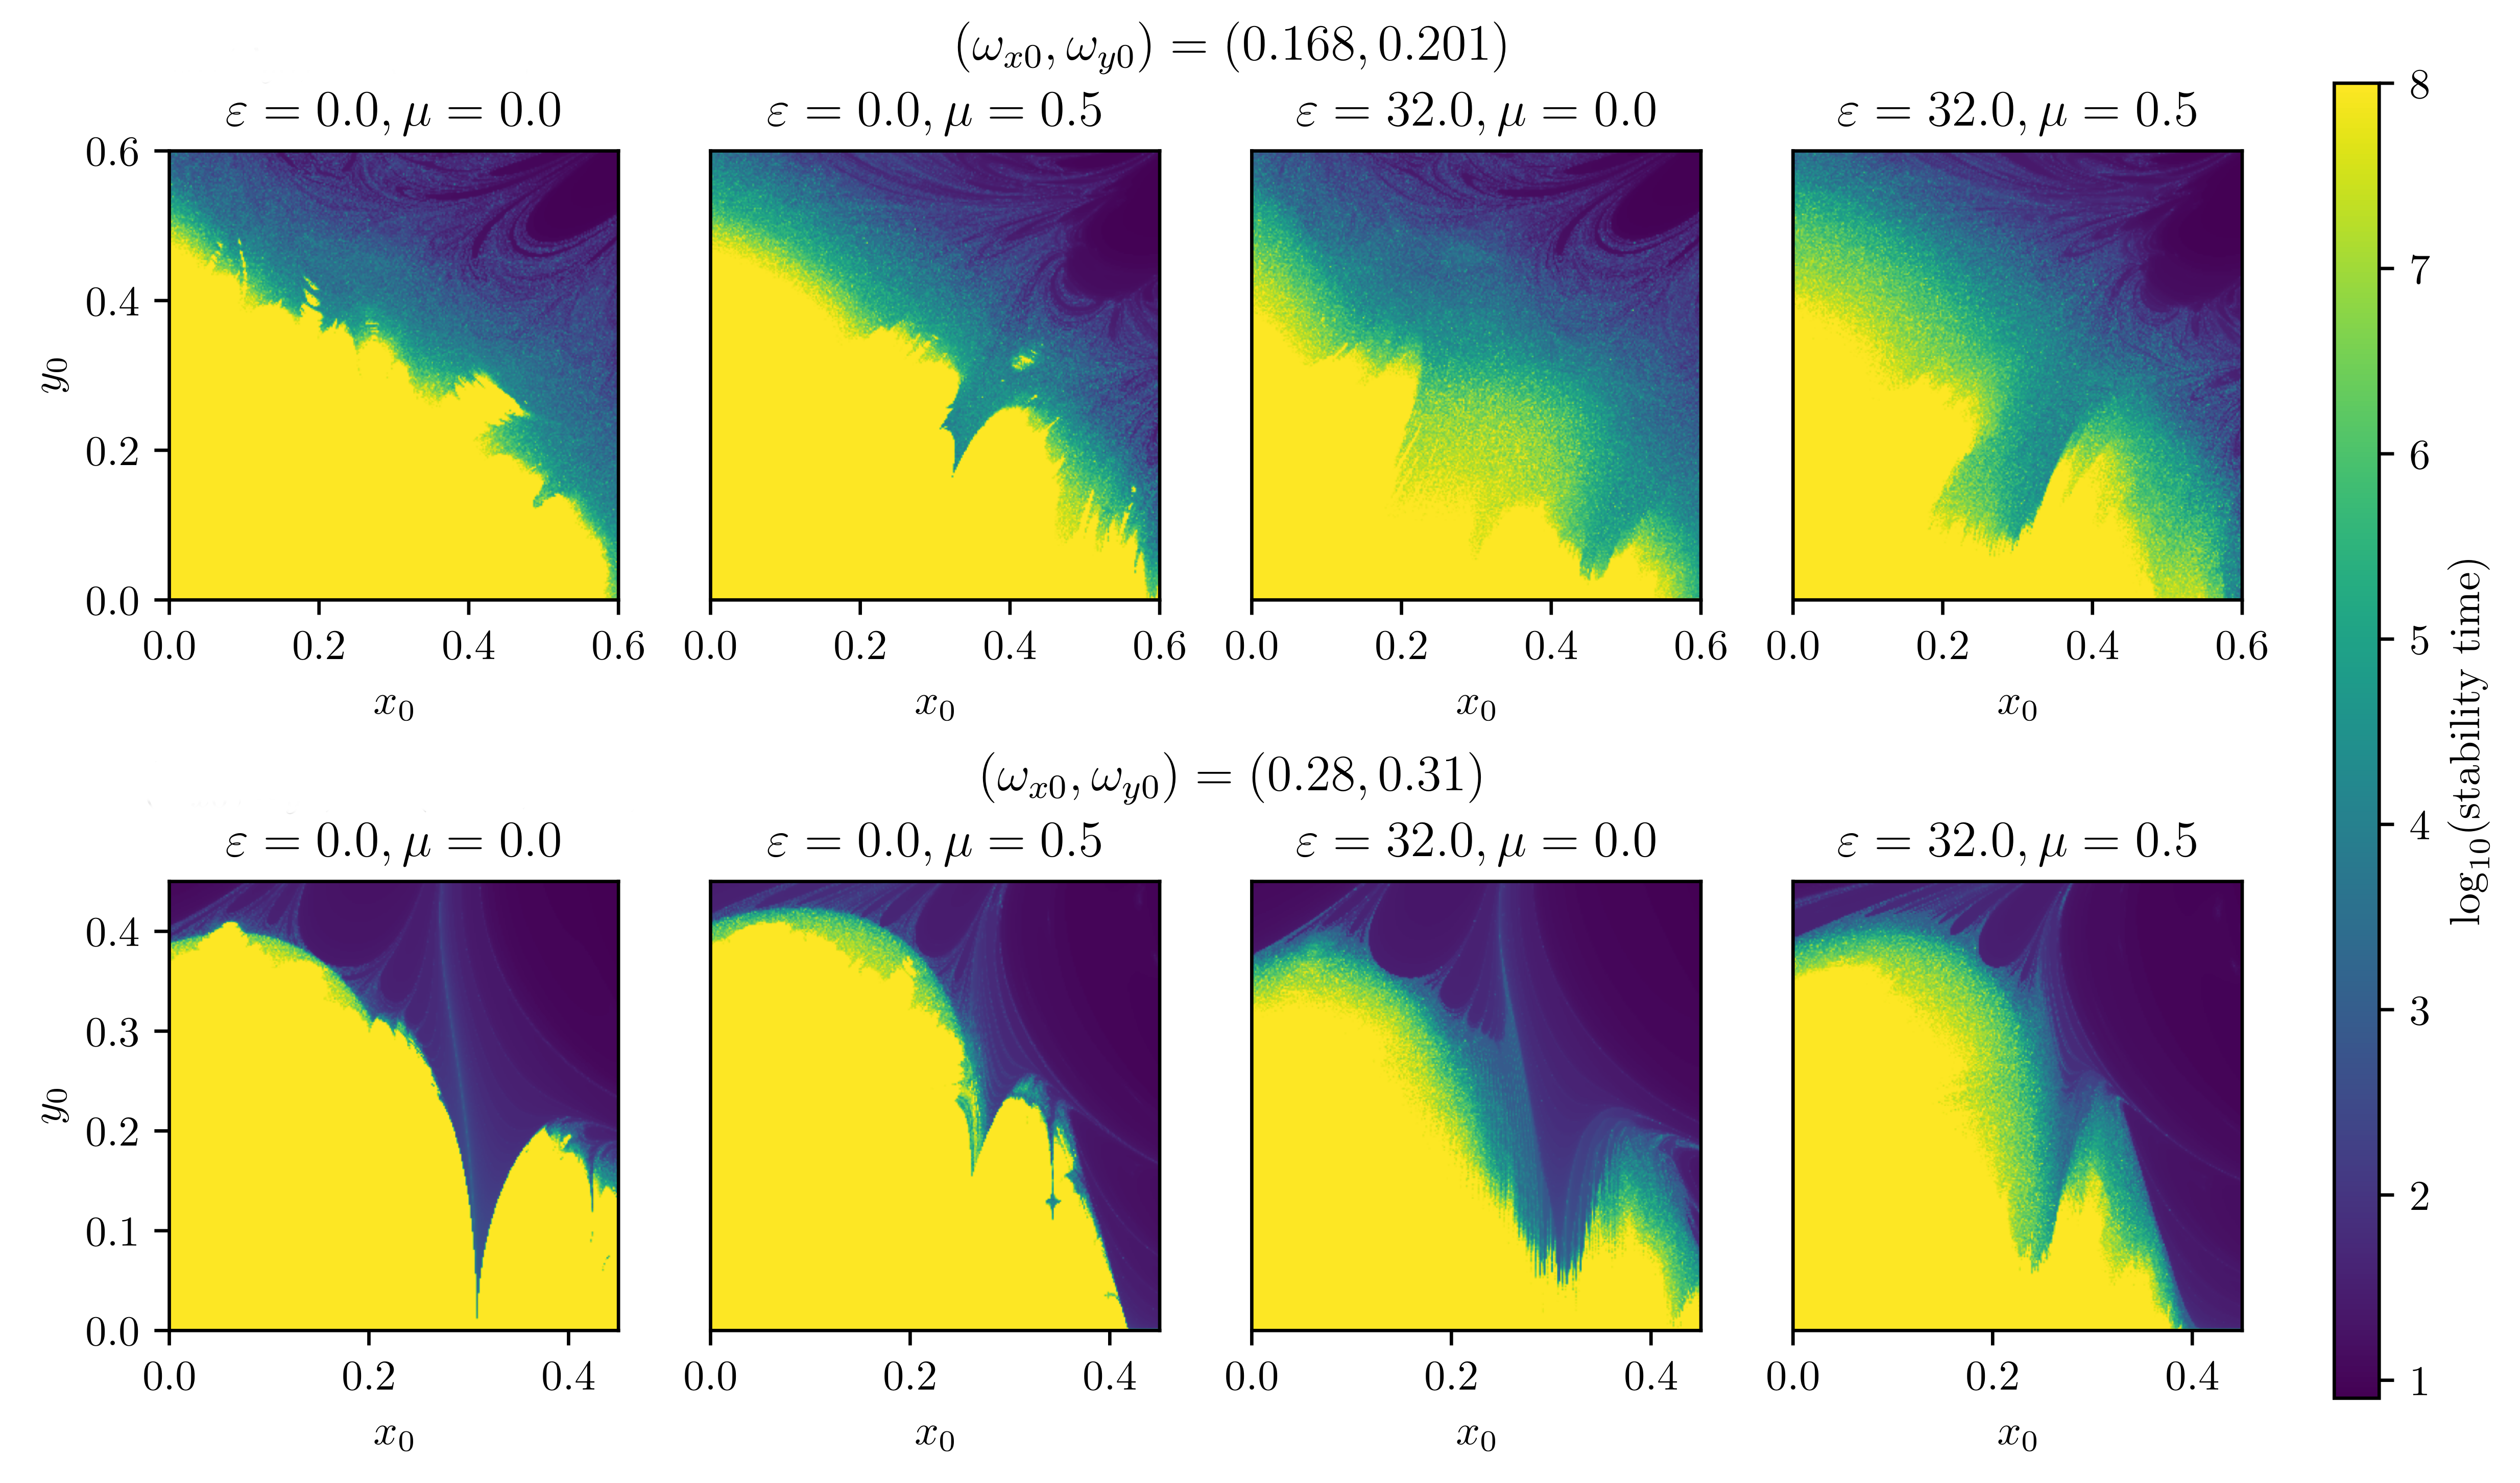
\includegraphics[width=\textwidth]{6_dynamic_indicators/fig/stability.png}
    \caption{Survival plot for various 4\textsc{d} modulated Hénon maps with quadratic and cubic non-linearities. Initial conditions, sampled on an uniform Cartesian $300\times300$ grid in the $x-y$ plane, are tracked up to $n_\text{max}=10^8$ and are considered lost when their distance to the origin exceeds a predefined maximum radius $r_\mathrm{c}=10^2$. The two sets of linear frequencies feature different shapes of the stable region as can be seen by comparing the plots in the two rows. The parameters $\varepsilon$ and $\mu$ induce additional changes, in particular the increase of the size of the transition region between stability up to $n_\mathrm{max}$ and shorter stability time. The color scale is related to the logarithm of the stability time as reported on the right.}
    \label{fig:survival}
\end{figure*}
%
The two rows of Fig.~\ref{fig:survival} show the survival plots for the two sets of frequencies considered in the studies. The shape of the stable region (yellow area) strongly depends on the frequencies, as different sets of resonances affect the dynamics. Furthermore, the impact of $\varepsilon$ and $\mu$ is also clearly seen. The first enlarges the transition region between stable initial conditions and unstable ones, i.e., the region for which $n_\mathrm{stab} < n_\mathrm{max}$, where a weak diffusion occurs, while the latter changes the shape of the stable region.
%
\section{\label{sec:dyn:results} Results of numerical investigations}
%
In the following, we report the results of the numerical study of the dynamic indicators presented in Section~\ref{sec:dyn:review}, namely $\log_{10}(LE)$, $FLI$, $FLI^{WB}$, $MEGNO(LE)$, $GALI^{(4)}$, $REM$, and $FMA$. Note that we consider the logarithm of $LE$, as it is a quantity comparable to $FLI$ and $MEGNO(LE)$. We first focus on the dependence of $FLI$ on the choice of the initial displacement vector $\vb{\xi}$, and compare it with $\log_{10}(LE)$. Next, we discuss a comparison between the convergence rate of $FLI$ and that of $FLI^{WB}$. Finally, we compare the classification performance of all dynamic indicators by determining their accuracy, together with its time dependence, in reconstructing a Ground Truth (GT) evaluated at a high iteration time.
%
\subsection{Dependence on the initial displacement}

The main feature of $LE$, compared to $FLI$, is its independence from the initial choice of direction of the unitary displacement vector $\vb{\xi}$. To highlight this, in Fig.~\ref{fig:le_fli_compare_short_long}, we directly compare the calculated values of $\log_{10}(\log_{10}(LE)/n)$ with those of $\log_{10}(FLI/n)$, calculated with an initial displacement along one of the four orthonormal base vectors $\hat{x},\,\hat{p}_x,\,\hat{y},\,\text{and }\hat{p}_y$. These calculations are carried out for a set of $300\times300$ initial conditions, sampled on a uniform Cartesian grid in the $x-y$ plane. It is possible to see how, at low turn number ($n=10^2$, top row), the different choice of displacement highlights the structures in $FLI$ that are missing in $LE$. This can be explained by considering that the displacement vector is not fully aligned along the largest Lyapunov exponent yet. In contrast, these structures are missing for $LE$, which has smoother behaviour.

\begin{figure*}[th]
    \centering
    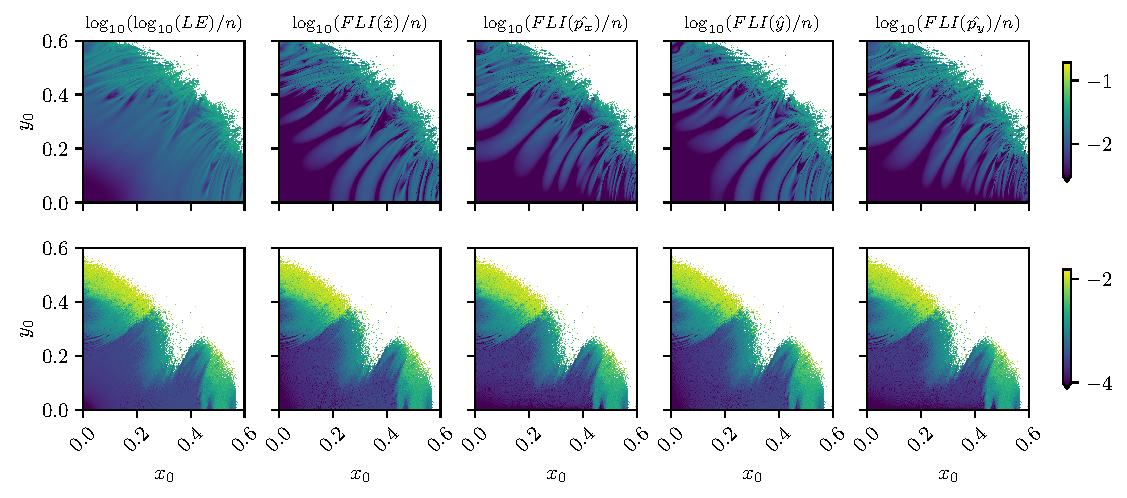
\includegraphics[width=\textwidth]{6_dynamic_indicators/fig/corrected_figs/LE_FLI_NEO.pdf}
    % 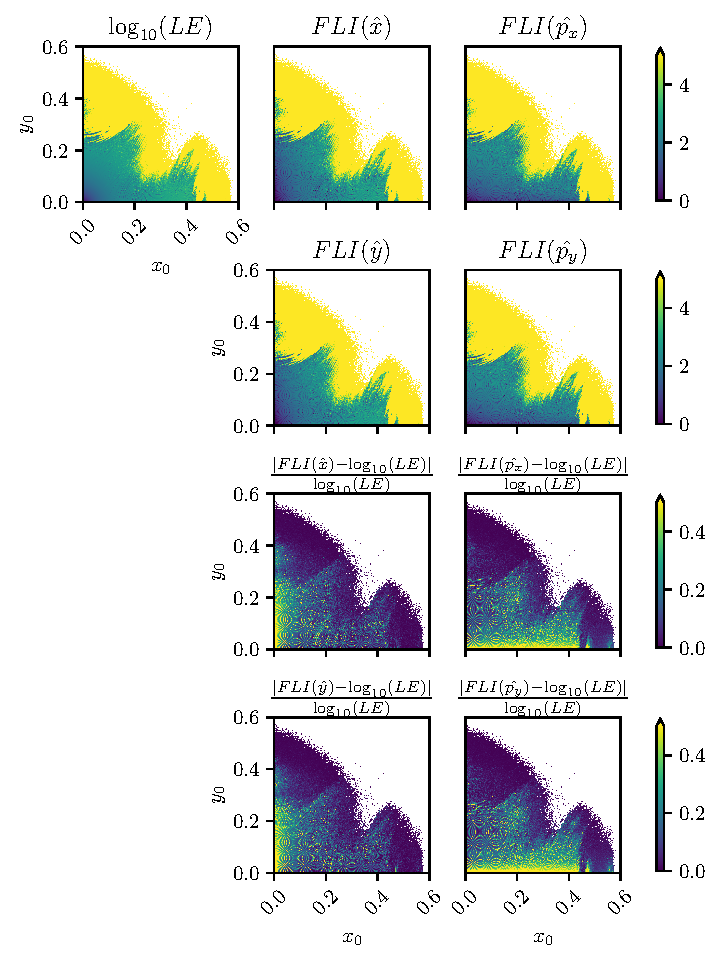
\includegraphics[width=0.6\textwidth]{6_dynamic_indicators/fig/LE_FLI_high.pdf}
    \caption{Color maps of $\log_{10}(\log_{10}(LE)/n)$ and $\log_{10}(FLI/n)$ indicators for a low iteration number ($n=10^2$, top row) and a high iteration number ($n=10^4$, bottom row). In both rows, the $FLI$ for the four possible displacements are shown together with $LE$, in order to highlight the different structures shown by the indicators. It is possible to see how, for low iteration numbers, different choices of initial displacement for $FLI$ highlight structures that do not appear in $LE$. The differences reduce for higher number of turns, but are still present. Note that an arrow at the bottom of the color bar means that pixels of the bottom color correspond to a value equal to or lower than the bottom value. White pixels correspond to initial conditions whose distance from the origin has exceeded a predefined radius ($r_c=10^2$) during the tracking, before reaching the target iteration number $n$. (Simulation parameters used: $(\omega_{x0},\omega_{y0})= (0.168,\ 0.201),\ \varepsilon=64.0,\ \mu=0.5$).}
    \label{fig:le_fli_compare_short_long}
\end{figure*}

%\begin{figure}[htp]
%    \centering
%    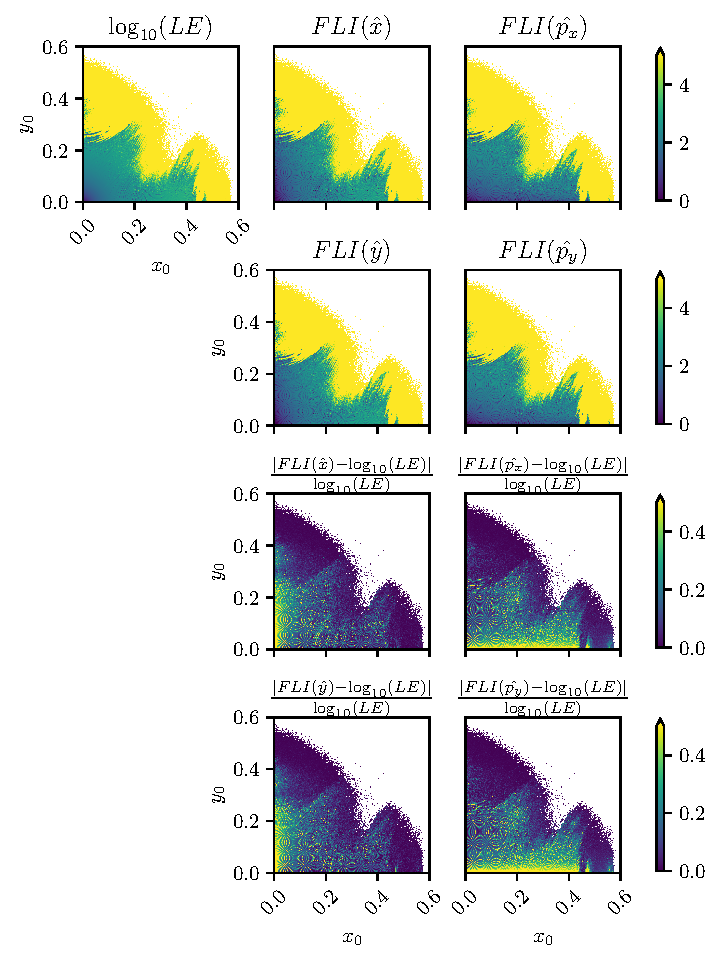
\includegraphics[width=0.6\textwidth]{6_dynamic_indicators/fig/LE_FLI_high.pdf}
%    \caption{Colormaps of $LE$ and $FLI$ for a high %iteration number $(n=10^4)$. Differently from %Fig.~\ref{fig:le_fli_compare_short}, a rather similar %structure is defined by the various dynamic indicators. %An arrow at the top of a colorbar means that pixels of %top color are either greater or equal the top value. %$\left((\omega_{x0},\omega_{y0})= (0.168,\ 0.201),\ %\varepsilon=64.0,\ \mu=0.5 \right)$.}
%    \label{fig:le_fli_compare_long}
%\end{figure}

The observed differences are greatly reduced for a higher number of turns ($n=10^4$, bottom row), as the initial displacement tends to become almost aligned along the direction corresponding to the largest Lyapunov exponent. However, despite the smaller differences between $\log_{10}(\log_{10}(LE)/n)$ and $\log_{10}(FLI/n)$, the behaviour of the various indicators is still not the same. It is worth noting how displacements along $\hat{x}$ and $\hat{y}$ produce similar structures that are, however, different with respect to the case in which displacement is carried out along $\hat{p}_x$ or $\hat{p}_y$. Globally, these observations underline the value of the invariance properties of $LE$, which seems to be more promising than $FLI$ for the analyses that will be discussed in the following sections.

As this dependence on the initial displacement decreases with higher iteration numbers, we will focus only on $FLI(\hat{x})$ for the remainder of the chapter, as the rest of the results are not significantly affected by this choice.

% This evaluation eventually highlights the presence of a bimodal distribution, with one ensemble of regular initial conditions and one of chaotic ones.
%
\subsection{Application of Weighted Birkhoff averaging to $FLI$}\label{subsec:dyn:FLI:WB}
%
As an additional analysis of the time dependence of chaos indicators, we compare the values obtained for $FLI$ at different times, using the standard approach that considers the mean in Eq.~\eqref{eq:fli_mean}, that is, $FLI/n$, or the variant based on the use of Birkhoff weights as in Eq.~\eqref{eq:fli_birkhoff}, that is, $FLI^{WB}$. The analysis starts considering two ensembles of regular and chaotic particles that have been classified by means of the value of the $FLI$ indicator computed for $n=10^8$ turns (effectively this sets a ground-truth level, as discussed in the next section). The sets are also used to calculate the time evolution of $FLI/n$ and $FLI^{WB}$ with the objective of evaluating possible improvements in the latter compared to the first. In Fig.~\ref{fig:fli_compare_mean_birk} (top), the comparison is made for a subset of the set of regular initial conditions, whereas the behaviour of chaotic ones is shown in the bottom plot of the same figure. It is possible to observe how, for regular initial conditions, Birkhoff averaging consistently speeds up the convergence of $FLI^{WB}$ to zero.

\begin{figure}[htp]
    \centering
    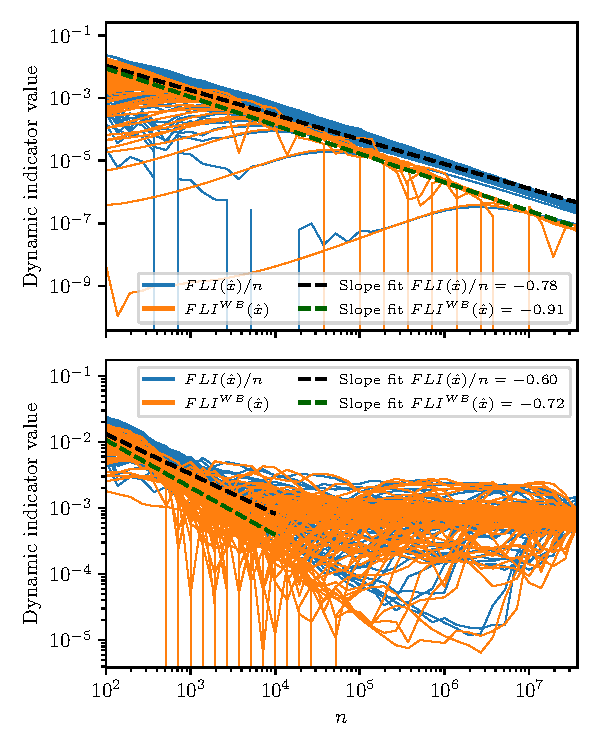
\includegraphics[width=0.8\textwidth]{6_dynamic_indicators/fig/lyap_birkhoff.pdf}
    \caption{Time evolution of $FLI$ computed using either a standard mean or the Birkhoff averaging. Top plot: indicators computed for a set of 100 regular initial conditions, the fit highlights a faster convergence rate for the Birkhoff averaging. Bottom plot: indicators computed for a set of 100 chaotic initial conditions. A similar improvement in convergence rate is observed for low $n$ values, before reaching a saturation value of the indicator of the order of $10^{-3}$. (Simulation parameters: $(\omega_{x0},\omega_{y0})= (0.28,\ 0.31),\ \varepsilon=32.0,\ \mu=0.5$).}
    \label{fig:fli_compare_mean_birk}
\end{figure}

The case of chaotic initial conditions has different characteristics. In fact, a saturation region is observed for the indicator value on the order of $10^{-3}$ for both indicators. When this value is reached, both indicators oscillate around it. However, the slope with which this non-zero value is reached is different for the two indicators and is higher in absolute value for $FLI^{WB}$ than for $FLI/n$, similar to what is observed for the case of regular orbits. It is also worth stressing the presence of initial conditions that, up to some $n=10^6$ turns, feature a steady decrease in the value of the dynamic indicator, as if they were characterized by regular motion. However, after that, the value of the indicator suddenly increases, reaching the value that identifies chaotic orbits. This behaviour clearly defies any approach aimed at classifying initial conditions as regular or chaotic in finite time. 

The improvement caused by the Birkhoff averages is also clearly visible in Fig.~\ref{fig:fli_colormap_mean_birk}, where the time evolution of the distribution of the values of $FLI/n$ (top) and $FLI^{WB}$ (bottom) is shown. The part of the distribution corresponding to the regular initial conditions reaches its peak (yellow band) and moves toward zero with increasing $n$. However, the displacement towards zero is faster for $FLI^{WB}$. Furthermore, the peak of the distribution is sharper for $FLI^{WB}$ than for $FLI$. In both graphs, a faint trace of a peak is visible corresponding to the indicator value of about $10^{-3}$. This feature is remarkably similar for the two indicators, as already seen in Fig.~\ref{fig:fli_colormap_mean_birk}.

\begin{figure}[htp]
    \centering
    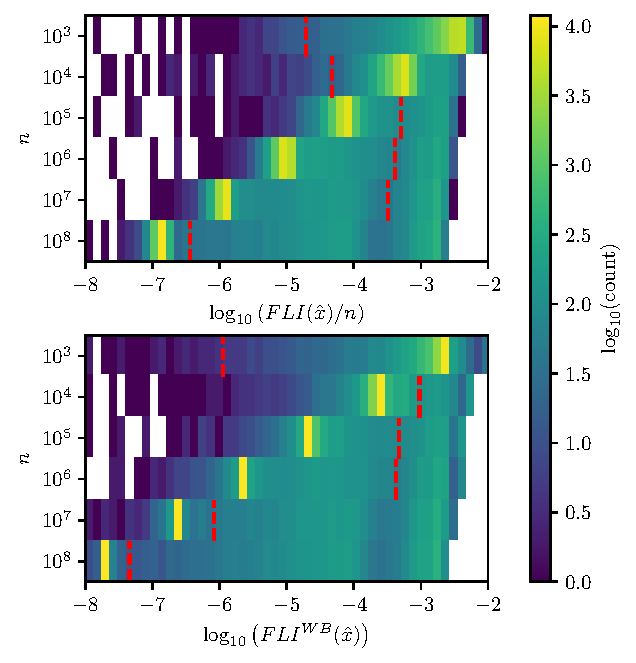
\includegraphics[width=0.8\textwidth]{6_dynamic_indicators/fig/lyapunov_birkhoff_map.pdf}
    \caption{Time evolution of the distribution of the values of $FLI$ (top) and $FLI^{WB}$ (bottom) indicators for the whole set of 15684 initial conditions that survived up to $n_\text{max}=10^8$. The Birkhoff averaging leads to faster convergence towards zero of the regular initial conditions, which are represented by the yellow band. Furthermore, the width of such a band is narrower for $FLI^{WB}$ with respect to $FLI$. The red dashed lines represent threshold values, defined by our algorithm, representing the attempt to perform the binary classification in regular and chaotic initial conditions. (Simulation parameters: $(\omega_{x0},\omega_{y0})= (0.28,\ 0.31),\ \varepsilon=32.0,\  \mu=0.1$).}
    \label{fig:fli_colormap_mean_birk}
\end{figure}

This behaviour shows that the regular orbits benefit from the use of the Birkhoff averages, whereas the chaotic ones are mostly unaffected by the special averaging mechanism. These features can be exploited for the classification problem that will be addressed in the next section.

\subsection{Classification performance}\label{subsec:dyn:classification}

For this analysis, we study the predictive performance of chaos indicators in terms of a binary classification of a large set of initial conditions by varying the number of iterations $n$. It should be stressed that this classification only concerns the behaviour of an orbit that has been detected to be stable for $n_\mathrm{max}$.

An overview of the time dependence of the dynamic indicators and the distribution of their values observed in our numerical investigation is given in the Appendix~\ref{app:timedep}. The main feature of interest, which constitutes the basis of this analysis, is the general tendency of dynamic indicators to create a bimodal distribution, as has also been reported for finite-time Lyapunov exponents in~\cite{PhysRevE.60.2761,VALLEJO200326}. We focus on studying the evolution of this specific characteristic, i.e., the presence of two peaks in the distribution of indicator values, as a function of time, which is the key feature used for the classification analysis.

As the development of the bimodal distribution requires various orders of magnitude of the number of turns, we perform our analysis on the logarithm of the seven dynamic indicators, namely $\log_{10}(\log_{10}(LE)/n)$, $\log_{10}(MEGNO(LE)/n)$, $\log_{10}(FLI/n)$, $\log_{10}(FLI^{WB})$, $\log_{10}(GALI^{(4)})$, $\log_{10}(REM)$, and $\log_{10}(FMA)$. The factor $n^{-1}$ is included in the first two indicators to observe a comparable evolution of values over time with the two $FLI$ indicators, since, ultimately, its presence does not alter the outcome of these studies.

To carry out this task, we first construct a ground truth (GT) for different sets of parameters for the 4\textsc{d} Hénon map, iterated for $n_\text{max} = 10^8$. The initial conditions are then classified into a binary chaotic/regular classification scheme using the $LE$ indicator. An example is given in Fig.~\ref{fig:ground_truth_bis} where eight cases, the same as those depicted in Fig.~\ref{fig:survival}, are displayed. Dark colours identify regular regions of the phase space, whereas lighter colours denote chaotic regions. It is clearly seen that the frequency modulation and the presence of the cubic non-linearity increase the extent of the chaotic areas of the phase space, also generating regions in which regular and chaotic orbits are deeply intertwined.  

\begin{figure*}[th]
    \centering
    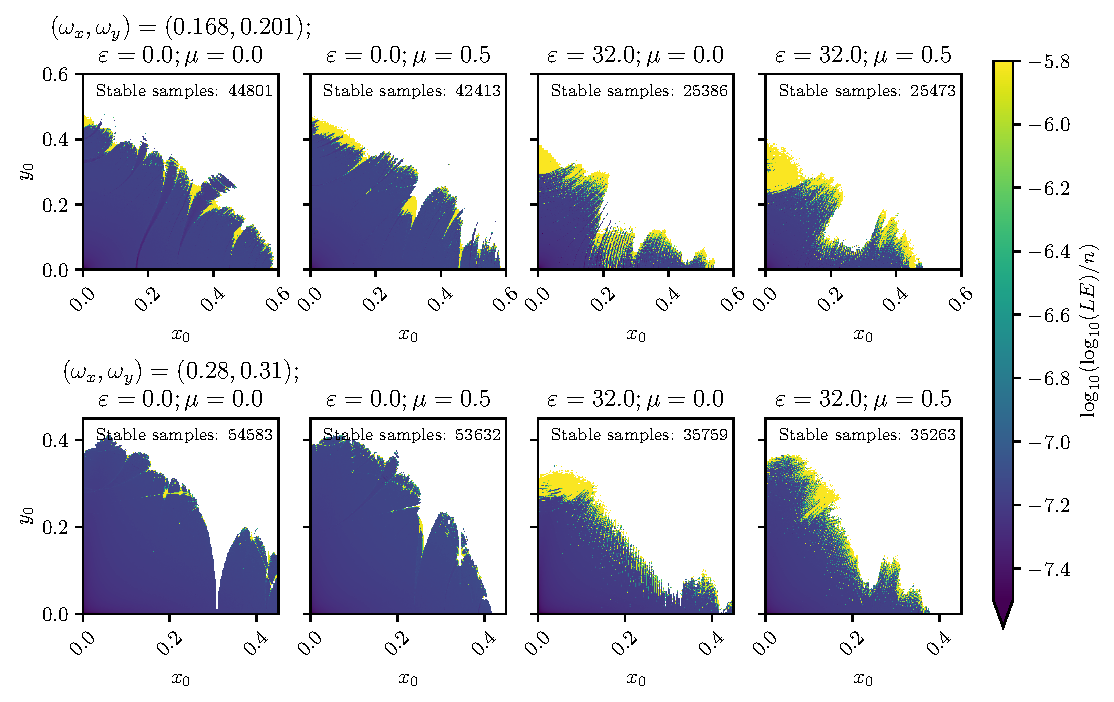
\includegraphics[width=\textwidth]{6_dynamic_indicators/fig/gt_example_colormap.pdf}
    \caption{Distributions of $\log_{10}(\log_{10}(LE)/n)$ for various 4\textsc{d} modulated Hénon maps (the same cases shown in Fig.~\ref{fig:survival}) with quadratic and cubic non-linearities. $300\times300$ initial conditions, sampled on an uniform Cartesian grid in the $x-y$ plane, are tracked up to $n_\text{max}=10^8$. It is possible to observe how the case for $\varepsilon=0.0,\ \mu=0.0$, corresponding to the absence of modulation and cubic non-linearities, lead to regular motion almost everywhere, except for a small set of initial conditions. For the other cases, extended regions of chaotic motion are visible. Note that the maximum value registered in the color maps corresponds to numerical saturation.}
    \label{fig:ground_truth_bis}
\end{figure*}

The GT classification is built from the distribution of the values of $\log_{10}(\log_{10}(LE)/n)$ for $n_\text{max}$. The resulting distribution has a main group of regular initial conditions with low value $LE$, and a second group of chaotic initial conditions with higher value $LE$. Due to the large separation of these two clusters, a threshold value has been calculated to distinguish them using a kernel density estimation method (KDE)~\cite{doi:10.1080/24709360.2017.1396742, refId0} with a Gaussian kernel and different bandwidth values. This allows investigating the Mode Tree~\cite{10.2307/1390955} of the distribution, detecting its two main modes, and setting the position of the minimum of the distribution between them. It is worth stressing that more refined approaches might be devised to detect the peaks or, equivalently, cluster the indicator values, but they have not been considered in this analysis. In fact, our focus is on the performance of the indicator in generating a suitable distribution for the classification problem, even for low values of $n$, not on designing a sophisticated algorithm to analyse the distribution of the indicator, including its peculiarities.

An example of the GT construction process can be seen in Fig.~\ref{fig:ground_truth_2}. 
%
\begin{figure*}[htp]
    \centering
    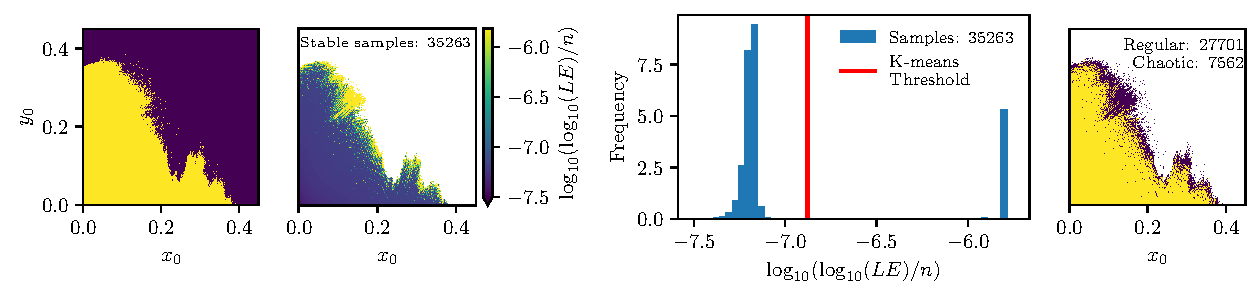
\includegraphics[width=1.0\textwidth]{6_dynamic_indicators/fig/GT.pdf}
    \caption{Ground Truth construction for a modulated Hénon map. From left to right: a survival plot of the initial conditions stable up to $n_\text{max}=10^8$ (yellow is stable, purple is unstable); distribution of the $LE$ indicator for all stable initial conditions, evaluated at $n_\text{max}$; histogram of $\log_{10}(\log_{10}(LE)/n)$, classified with a threshold evaluated with a KDE-based procedure; binary classification of regular (yellow) and chaotic (purple) initial conditions. (Simulation parameters:  $(\omega_{x0},\omega_{y0})= (0.28,\ 0.31),\ \varepsilon=32.0,\ \mu=0.5$).}
    \label{fig:ground_truth_2}
\end{figure*}
%
Stable initial conditions up to $n_\mathrm{max}$ are identified by direct tracking (first graph from the left), and the value of the indicator $LE$ is calculated for the set of stable initial conditions (second graph from the left). At this stage, it is possible to compute the distribution of $LE$ and determine the threshold that separates the peaks of the bimodal distribution (third plot from the left) and provides the criterion to classify any given initial condition as regular of chaotic. Applying the computed threshold, it is possible to generate a binary map with the resulting classification (fourth plot from the left). The determination of the threshold for the case shown is rather straightforward, as the large separation between the two peaks makes the actual value of the threshold not particularly relevant. However, when $n \ll n_\mathrm{max}$ the separation between the peaks decreases and the threshold value becomes essential for an efficient classification of the initial conditions. 

Examples of the procedure for determining the threshold based on the indicator distribution are shown in Fig.~\ref{fig:thresholds}. In the top plot, the case of $REM$ is depicted (but it is representative of all other indicators except $FMA$). The use of KDE with different bandwidth clearly shows how the two peaks of the distribution can be detected. This allows the position of the threshold to be set at the location of the minimum value of the distribution in between the two peaks. The case of $FMA$ is different since the distribution has three peaks and the standard algorithm to determine the threshold must be adapted. Therefore, KDE is used to determine the position of the three peaks, and the threshold is set at the position of the minimum of the distribution in between the two peaks with the largest amplitude.  

This choice is somewhat arbitrary, but the features of the distribution clearly indicate that the performance of the indicator is limited, with little possibility of improving it. Indeed, the non-negligible fraction of initial conditions that generate the part of the distribution in between the extreme peaks cannot be clearly classified by the proposed approach, as some of them will turn chaotic, whereas other regular if the indicator would be computed over a longer time span.  

\begin{figure}[htp]
    \centering
    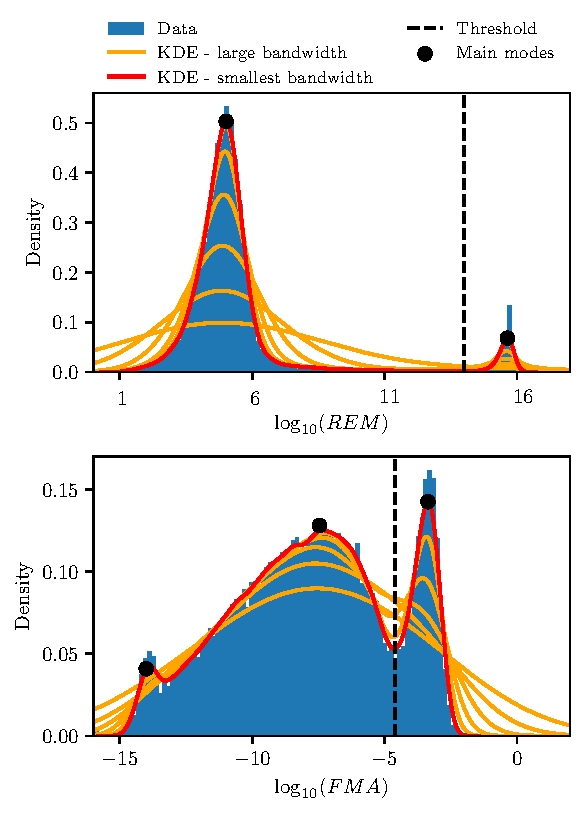
\includegraphics[width=0.7\textwidth]{6_dynamic_indicators/fig/edited_edited_thresholds.pdf}
    \caption{Example of the KDE-based procedure for computing a threshold for the binary classification (regular/chaotic) of initial conditions. Top: application to $\log_{10}(REM)$ (evaluated at $n=10^5$). KDEs with various bandwidth are used until the two main peaks of the bi-modal distribution are detected, the threshold is then placed at the position of the minimum of the distribution between them. This procedure is applied to all dynamic indicators except for $FMA$. Bottom: application of the procedure to $\log_{10}(FMA)$ (evaluated at $n=10^5$), which clearly exhibits a three-mode distribution. The procedure is applied so that it detects the three main modes of the distribution, and then sets the threshold at the minimum of the distribution between the two modes at higher values. (Simulation parameters:  $(\omega_{x0},\omega_{y0})= (0.28,\ 0.31),\ \varepsilon=32.0,\ \mu=0.5$).}
    \label{fig:thresholds}
\end{figure}

Once the GT has been computed, we define as predictive performance of a dynamic indicator the accuracy in reconstructing the binary classification in the GT, that is, the ratio between the correctly labelled initial conditions and the total number of stable initial conditions. Such a reconstruction is attempted using the same strategy implemented for the determination of the GT, namely, we consider the distribution of the dynamic indicator under consideration and define a binary classification using a threshold computed via the KDE-based approach. The resulting thresholds evaluated over time for $REM$ and $FMA$ are visualised in detail in Fig.~\ref{fig:neo_evolution}, while the results for the other dynamic indicators are presented in Appendix~\ref{app:timedep}.

\begin{figure*}[htp]
    \centering
    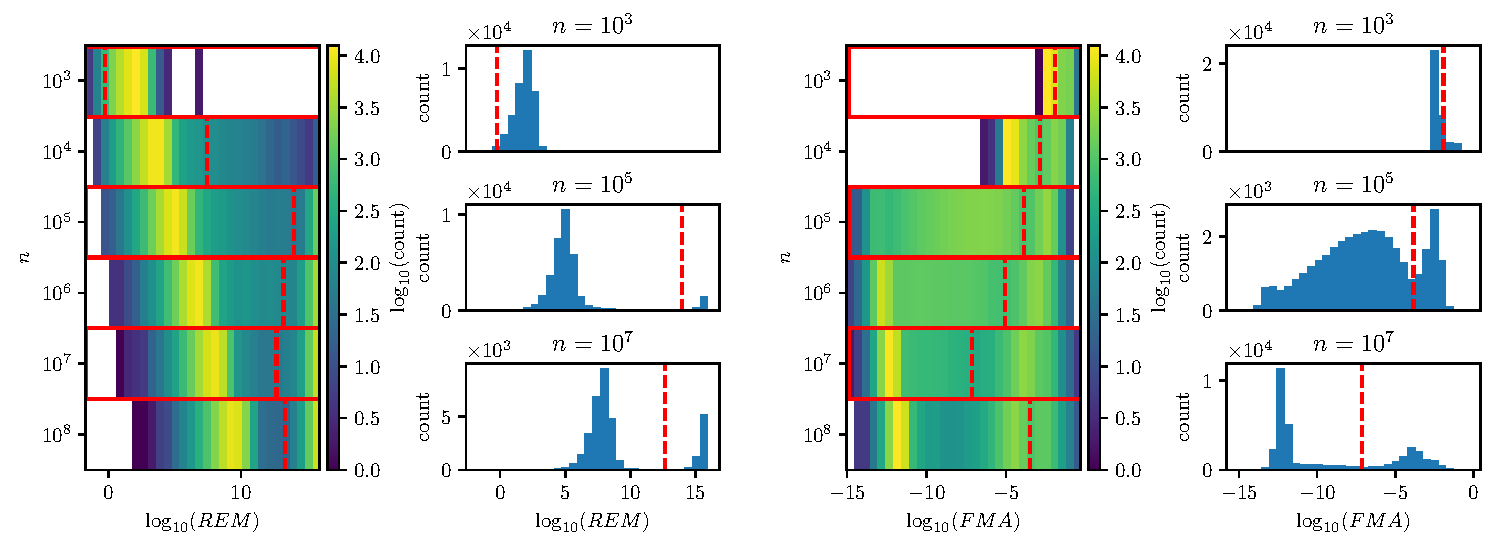
\includegraphics[width=1.0\textwidth]{6_dynamic_indicators/fig/corrected_figs/neo_evolution_idx_3.pdf}
    \caption{Distribution of values of $\log_{10}(REM)$ (left) and $\log_{10}(FMA)$ (right) as a function of time for a modulated 4\textsc{d} Hénon map. The red dashed lines represent threshold values, defined by our algorithm shown in Fig.~\ref{fig:thresholds}, representing our criterion to distinguish regular and chaotic orbits.
    For low values of the iterations $n$, the distribution of both indicators is in general represented by a uni-modal function. For higher values of $n$, we can see the formation of two separate clusters in the case of $REM$, making the distribution bi-modal. For $FMA$, we have in general a different behaviour, as it tends to form a tri-modal distribution. (simulation parameters: $(\omega_{x0},\omega_{y0})= (0.28,\ 0.31),\ \varepsilon=32.0,\ \mu=0.5$).}
    \label{fig:neo_evolution}
\end{figure*}

The accuracy performance of the dynamic indicator is then evaluated for various $n < n_{\text{max}}$. We expect a good-performing dynamic indicator to achieve high accuracy values when it generates two separate groups, even when $n \ll n_{\text{max}}$. Such behaviour, in fact, enables effective mode detection and consequent effective GT reconstruction. In contrast, a poor-performing dynamic indicator will need a longer tracking time before showing the presence of two separate clusters, causing the threshold determination to be unable to separate the chaotic from the regular initial conditions.

A global comparison of the classification performance of the seven dynamic indicators is carried out, and the accuracy achieved by the dynamic indicators as a function of $n$ is shown in Fig.~\ref{fig:performance}, for different sets of parameter values for the 4\textsc{d} Hénon maps. 

\begin{figure*}[th]
    \centering
    %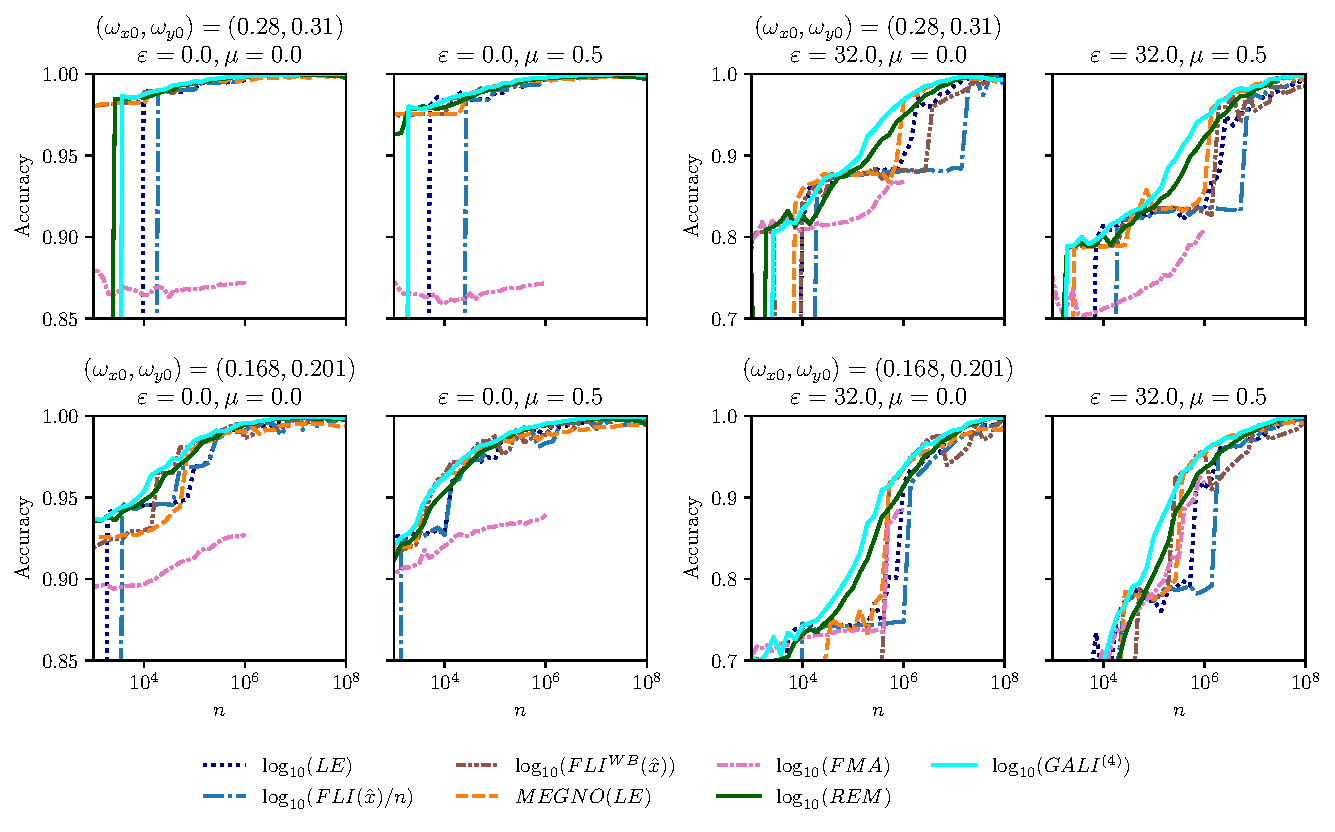
\includegraphics[width=1.0\textwidth]{6_dynamic_indicators/fig/performance.pdf}
    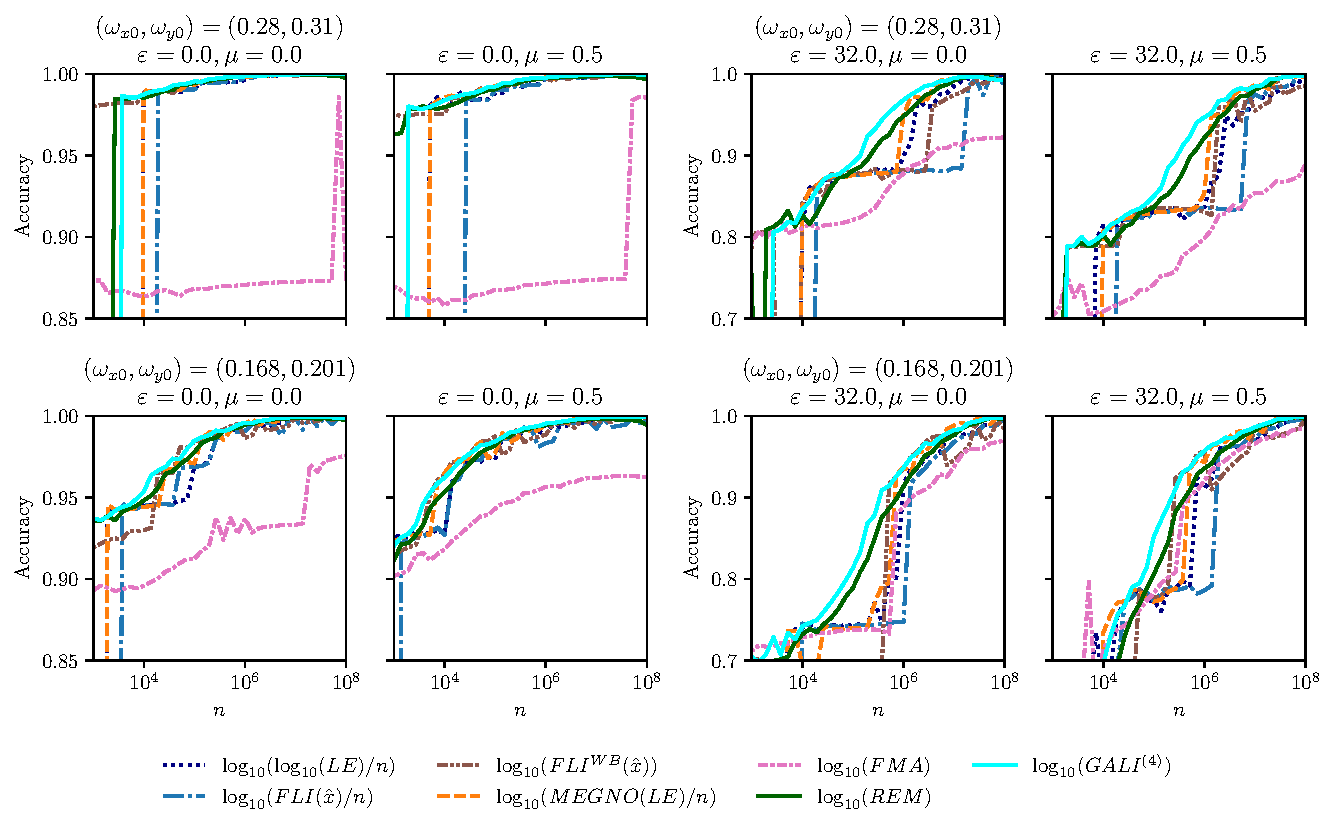
\includegraphics[width=1.0\textwidth]{6_dynamic_indicators/fig/corrected_figs/performance.pdf}
%    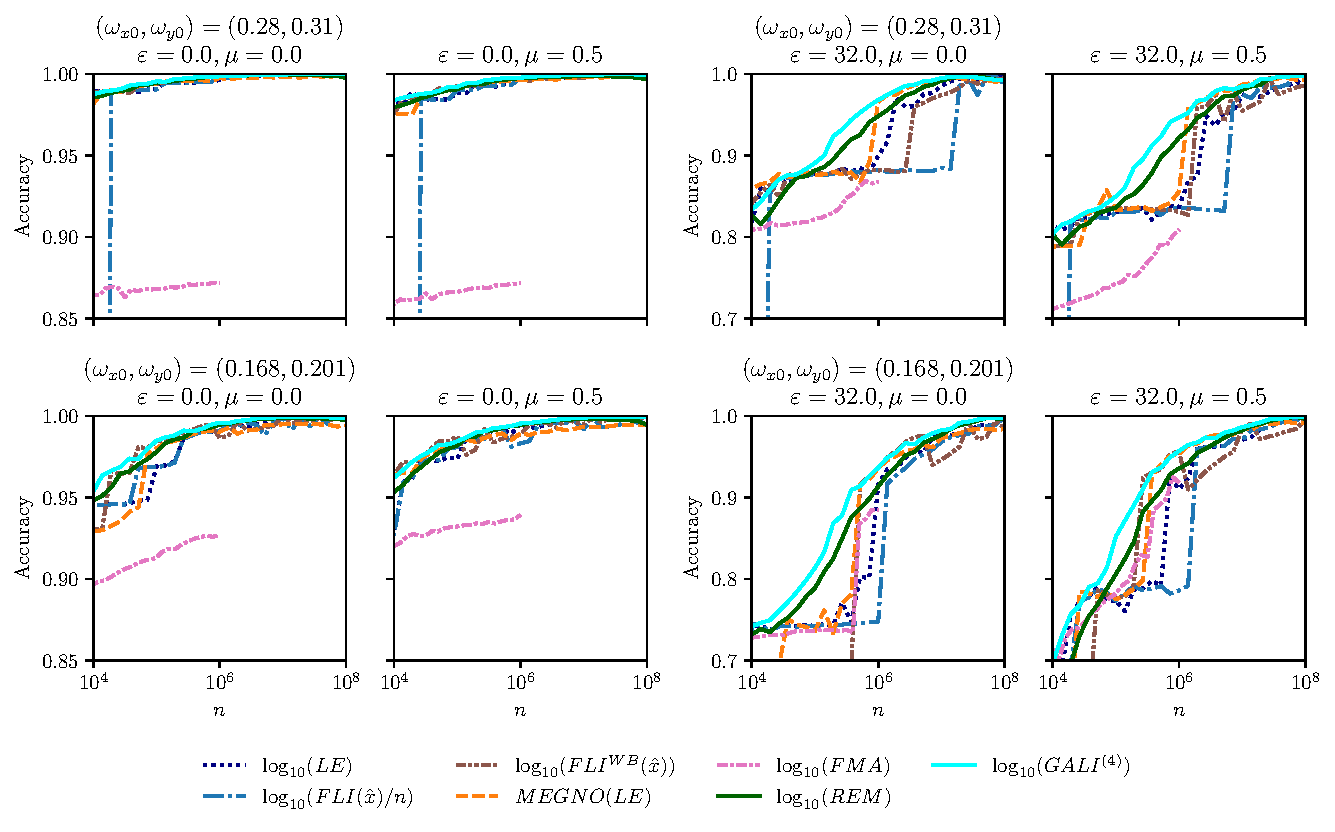
\includegraphics[width=1.0\textwidth]{6_dynamic_indicators/fig/performance_bis.pdf}
    \caption{Time dependence of the accuracy achieved in reconstructing the Ground Truth (computed for $n_\text{max}=10^8$) by the various dynamic indicators for eight cases of the 4\textsc{d} modulated Hénon maps (the same cases shown in Fig.~\ref{fig:survival}), differing by cubic non-linearities and frequency modulation.}
    \label{fig:performance}
\end{figure*}

When considering the Hénon maps with $\varepsilon=0.0$, i.e., without frequency modulation, a rather small fraction of chaotic orbits with a very mild dependence on $n$ of the accuracy of the various dynamic indicators is observed. Furthermore, $FMA$ differs from all other indicators, clearly showing poorer performance in terms of accuracy. All other indicators have very similar performance, the only difference being in the time at which a steplike increase in accuracy is observed, which occurs for $n = 10^3 - 10^4$, corresponding to 4-5 orders of magnitude lower than $n_\text{max}$. This sudden increase in accuracy is related to the time required by dynamic indicators to generate a bimodal distribution that can be efficiently analysed using our KDE-based procedure. In this sense, it should be noted that $GALI^{(4)}$ is the most accurate indicator, as it reaches high accuracy values even at very low values of $n$ and the gradual increase does not occur in the range of $n$ shown in the graphs. In general, the behaviour observed for all indicators (except $FMA$) shows that a rather accurate prediction of GT can be achieved using the information provided by the indicators over a rather limited number of turns.

In the case with $\varepsilon=32.0$, i.e., with frequency modulation and a larger fraction of chaotic orbits, the situation changes dramatically. Accuracy depends rather strongly on $n$, suggesting that chaos detection requires a larger number of turns to be accurate. In terms of the ranking of the indicators, $FMA$ remains the worst (this is certainly true for case $(\omega_{x0}, \omega_{y0}=(0.28, 0.31)$, while for case $(\omega_{x0}, \omega_{y0}=(0.168, 0.201)$ a better performance is observed). $REM$ and $GALI^{(4)}$, are the best values in a wide range of values of $n$. Furthermore, they do not show any sudden jump in accuracy because of their well-behaved distribution. Finally, we remark that beyond $n = 10^6 - 10^7$, the precision of all indicators is very similar.

To provide a quantitative assessment of the performance of the dynamic indicators, we define a performance estimate as
\begin{equation}
    \frac{1}{2}\int_4^6 \text{Accuracy}(10^x) \,\mathrm{d}x \,,
    \label{eq:final_evaluation}
\end{equation}
i.e., the integral of the accuracy achieved and displayed in Fig.~\ref{fig:performance} normalized to the integral of the ideal case with unit accuracy throughout the turn interval. The reasons for such a definition are twofold: First, it avoids the possible bias introduced by indicators that are more efficient in detecting the chaotic behaviour at low number of turns but that are not so efficient afterwards; second, it probes the predictive power of the indicator by setting an upper bound that is lower than the turn number used for determining the GT. Equation~\eqref{eq:final_evaluation} has been numerically evaluated using the trapezoidal rule and considering 50 values of $n$ equally spaced on a logarithmic scale over the interval $10^4-10^6$.  The performance estimate values for the dynamic indicators for the various H\'enon maps are reported in Table~\ref{table:values}. 

\begin{table*}[htb]
    \centering
    \begin{adjustbox}{width=\textwidth,center}
    \begin{tabular}{lc|lc}
        \hline
        \multicolumn{4}{c}{$(\omega_x, \omega_y) = (0.28, 0.31)$} \\
         \multicolumn{2}{c|}{$\varepsilon = 0.0; \mu = 0.0$} & \multicolumn{2}{c}{$\varepsilon = 0.0; \mu = 0.5$} \\
        \hline
        $\log_{{10}}(GALI^{{(4)}})$ & $0.99700 \pm 0.00014$ & $\log_{{10}}(GALI^{{(4)}})$ & $0.9956 \pm 0.0002$ \\ 
        $\log_{{10}}(FLI^{{WB}}(\hat{{x}}))$ & $0.9966 \pm 0.0005$ & $\log_{{10}}(REM)$ & $0.99423 \pm 0.00004$ \\ 
        $\log_{{10}}(MEGNO(LE)/n)$ & $0.9965 \pm 0.0008$ & $\log_{{10}}(\log_{{10}}(LE)/n)$ & $0.99 \pm 0.03$ \\ 
        $\log_{{10}}(REM)$ & $0.99629 \pm 0.00003$ & $\log_{{10}}(FLI^{{WB}}(\hat{{x}}))$ & $0.99 \pm 0.10$ \\ 
        $\log_{{10}}(\log_{{10}}(LE)/n)$ & $0.99 \pm 0.05$ & $\log_{{10}}(FLI(\hat{{x}})/n)$ & $0.9080 \pm 0.0016$ \\ 
        $\log_{{10}}(FLI(\hat{{x}})/n)$ & $0.94 \pm 0.01$ & $\log_{{10}}(MEGNO(LE)/n)$ & $0.90 \pm 0.14$ \\ 
        $\log_{{10}}(FMA)$ & $0.8738 \pm 0.0005$ & $\log_{{10}}(FMA)$ & $0.8797 \pm 0.0004$ \\ 
        \hline
        \multicolumn{4}{c}{$(\omega_x, \omega_y) = (0.28, 0.31)$} \\
         \multicolumn{2}{c|}{$\varepsilon = 32.0; \mu = 0.0$} & \multicolumn{2}{c}{$\varepsilon = 32.0; \mu = 0.5$} \\
        \hline
        $\log_{{10}}(GALI^{{(4)}})$ & $0.9453 \pm 0.0014$ & $\log_{{10}}(GALI^{{(4)}})$ & $0.924 \pm 0.002$ \\ 
        $\log_{{10}}(REM)$ & $0.9329 \pm 0.0003$ & $\log_{{10}}(REM)$ & $0.9096 \pm 0.0003$ \\ 
        $\log_{{10}}(MEGNO(LE)/n)$ & $0.93 \pm 0.08$ & $\log_{{10}}(MEGNO(LE)/n)$ & $0.90 \pm 0.09$ \\ 
        $\log_{{10}}(\log_{{10}}(LE)/n)$ & $0.924 \pm 0.011$ & $\log_{{10}}(\log_{{10}}(LE)/n)$ & $0.888 \pm 0.015$ \\ 
        $\log_{{10}}(FLI^{{WB}}(\hat{{x}}))$ & $0.913 \pm 0.007$ & $\log_{{10}}(FLI^{{WB}}(\hat{{x}}))$ & $0.88 \pm 0.02$ \\ 
        $\log_{{10}}(FMA)$ & $0.869 \pm 0.003$ & $\log_{{10}}(FLI(\hat{{x}})/n)$ & $0.843 \pm 0.009$ \\ 
        $\log_{{10}}(FLI(\hat{{x}})/n)$ & $0.863 \pm 0.007$ & $\log_{{10}}(FMA)$ & $0.797 \pm 0.005$ \\ 
        \hline
        \hline
        \multicolumn{4}{c}{$(\omega_x, \omega_y) = (0.168, 0.201)$} \\
         \multicolumn{2}{c|}{$\varepsilon = 0.0; \mu = 0.0$} & \multicolumn{2}{c}{$\varepsilon = 0.0; \mu = 0.5$} \\
        \hline
        $\log_{{10}}(GALI^{{(4)}})$ & $0.9896 \pm 0.0004$ & $\log_{{10}}(GALI^{{(4)}})$ & $0.9909 \pm 0.0004$ \\ 
        $\log_{{10}}(REM)$ & $0.98682 \pm 0.00009$ & $\log_{{10}}(MEGNO(LE)/n)$ & $0.99 \pm 0.09$ \\ 
        $\log_{{10}}(FLI^{{WB}}(\hat{{x}}))$ & $0.986 \pm 0.002$ & $\log_{{10}}(REM)$ & $0.98850 \pm 0.00012$ \\ 
        $\log_{{10}}(\log_{{10}}(LE)/n)$ & $0.981 \pm 0.003$ & $\log_{{10}}(FLI^{{WB}}(\hat{{x}}))$ & $0.988 \pm 0.002$ \\ 
        $\log_{{10}}(FLI(\hat{{x}})/n)$ & $0.980 \pm 0.016$ & $\log_{{10}}(\log_{{10}}(LE)/n)$ & $0.99 \pm 0.07$ \\ 
        $\log_{{10}}(FMA)$ & $0.9319 \pm 0.0010$ & $\log_{{10}}(FLI(\hat{{x}})/n)$ & $0.980 \pm 0.015$ \\ 
        $\log_{{10}}(MEGNO(LE)/n)$ & $0.9 \pm 0.2$ & $\log_{{10}}(FMA)$ & $0.9510 \pm 0.0009$ \\ 
        \hline
        \multicolumn{4}{c}{$(\omega_x, \omega_y) = (0.168, 0.201)$} \\
         \multicolumn{2}{c|}{$\varepsilon = 32.0; \mu = 0.0$} & \multicolumn{2}{c}{$\varepsilon = 32.0; \mu = 0.5$} \\
        \hline
        $\log_{{10}}(GALI^{{(4)}})$ & $0.903 \pm 0.003$ & $\log_{{10}}(GALI^{{(4)}})$ & $0.914 \pm 0.003$ \\ 
        $\log_{{10}}(REM)$ & $0.8880 \pm 0.0004$ & $\log_{{10}}(REM)$ & $0.8915 \pm 0.0004$ \\ 
        $\log_{{10}}(MEGNO(LE)/n)$ & $0.87 \pm 0.09$ & $\log_{{10}}(MEGNO(LE)/n)$ & $0.89 \pm 0.11$ \\ 
        $\log_{{10}}(\log_{{10}}(LE)/n)$ & $0.863 \pm 0.016$ & $\log_{{10}}(FMA)$ & $0.881 \pm 0.007$ \\ 
        $\log_{{10}}(FLI(\hat{{x}})/n)$ & $0.849 \pm 0.012$ & $\log_{{10}}(\log_{{10}}(LE)/n)$ & $0.88 \pm 0.02$ \\ 
        $\log_{{10}}(FLI^{{WB}}(\hat{{x}}))$ & $0.849 \pm 0.007$ & $\log_{{10}}(FLI^{{WB}}(\hat{{x}}))$ & $0.870 \pm 0.012$ \\ 
        $\log_{{10}}(FMA)$ & $0.843 \pm 0.004$ & $\log_{{10}}(FLI(\hat{{x}})/n)$ & $0.850 \pm 0.017$ \\ 
        \hline
    \end{tabular}
    \end{adjustbox}
    \caption{Performance estimate of the dynamic indicators for the various Hénon map configurations, evaluated using Eq.~\eqref{eq:final_evaluation} over the interval $n=10^4-10^6$. Values are ranked in decreasing order. It is clearly seen that $GALI^{(4)}$ is the highest scorer and $REM$ is the second-best scorer in most of the cases considered. The uncertainty in the performance estimate is evaluated by applying a variation of the calculated thresholds of $\pm 5\%$.}
    \label{table:values}
\end{table*}

Performance estimates have been ranked in decreasing order, separating the various cases considered in our analyses. $GALI^{(4)}$ turns out to be the highest scorer in all cases, followed by $REM$. Then we find $MEGNO$ and $FLI^{{WB}}(\hat{{x}})$, while $FMA$ tends to be the last in this ranking. The error associated with each performance estimate value is provided by the variation of the accuracy whenever the automatic threshold value is varied by $\pm 5\%$. This quantity provides information on the robustness of the accuracy against perturbation of the threshold: A small value indicates a high stability of the numerical values. It is also worth noting that the performance estimates of the best dynamic indicators are correlated with small values of the corresponding error.

Important insights on the performance of the various indicators can be gained by looking at the relative identification error in terms of false positive, i.e., when a regular orbit is classified as chaotic, and false negative, i.e., when a chaotic orbit is classified as regular. A false negative is almost unavoidable, according to the behaviour shown in Fig.~\ref{fig:fli_compare_mean_birk}, unless the indicator is calculated over a very large number of turns, which means accepting a very limited predictive power of the indicator. However, the behaviour of the two types of errors reveals interesting features of the various indicators. An overview of the dependence of false positive and false negative errors is shown in Fig.~\ref{fig:error_comparison}, where relative errors are displayed as functions of the turn number for the map configurations considered in the first row of Fig.~\ref{fig:performance}. 
%
\begin{figure*}[htp]
    \centering
    %\includegraphics[width=1.0\textwidth]{6_dynamic_indicators/fig/performance_specific_1_3.pdf}
    \includegraphics[width=\textwidth]{6_dynamic_indicators/fig/corrected_figs/performance_specific_1_3.pdf}
    \caption{Identification errors for the various indicators as a function of the number of turns for the cases displayed in the first row of Fig.~\ref{fig:performance}.}
    \label{fig:error_comparison}
\end{figure*}
%

The behaviour of the false positive error reveals a fundamental difference between $FMA$ and the other indicators. In fact, $FMA$ shows an error value that is only slightly dependent on the turn number and drops to small values for very large $n$. For the other indicators, for a low number of turns, this type of error is large, and then, around $10^4$ turns, it drops essentially to zero. This feature is related to the fact that, for a low number of turns, the bimodal structure is not yet present. It is also worth noting that, for the case of $FLI^(\hat{{x}})$ the Birkhoff averaging introduces a clear improvement by pushing the position of the sudden drop to zero of the false positive error to a lower number of turns.

The false negative error increases sharply at a turn number close to that corresponding to the abrupt decrease in the false positive error. After this turn number, two behaviours are observed: In the first case, the error level is approximately constant until it drops to a low value after $n \approx 10^7$. This value is relatively close to that used to determine the GT, which indicates a limited predictive power of the indicator. In the second case, the error level decreases almost linearly as a function of $n$. This is the key to achieving good performance and is the feature shown by $REM$ and $GALI^{(4)}$. It should be noted that $FMA$ also behaves in this way, i.e., with a linear decrease in the false positive error. However, when the false negative error drops, a jump in the false positive error is observed. This error then shows a decrease that is almost negligible up to $n_\mathrm{max}$. These characteristics, related to the characteristics of the distribution of the $FMA$ values, prevent this indicator from reaching a good performance level. 

As a last comment, these features are always present, but frequency modulation strongly enhances the errors. 
%
\section{\label{sec:dyn:conc} Conclusions}
%
In this chapter, various numerical indicators to identify the chaotic character of orbits of Hamiltonian systems have been presented and discussed in detail. The powerful Birkhoff averages were used to improve the convergence rate of an indicator in the case of regular initial conditions. The goal of our analysis is to evaluate the performance of the indicators in terms of accuracy in the binary classification of an orbit identified by its initial conditions, as regular or chaotic. An important element in this assessment is whether the correct classification can be achieved by using the information over a limited number of turns, i.e., whether an early chaos detection can be effectively performed, which is equivalent to probing the predictive power of dynamic indicators. 

The dynamical system that has been selected as a test bed for performance analyses is a 4\textsc{d} H\'enon-like symplectic map, with or without cubic non-linearity and with or without frequency modulation. This choice is justified by the relevant applications of this map to understand long-term stability problems in particle accelerators. Several configurations have been considered and, for each case, a ground truth classification has been determined with $n=10^8$ iterations. The various indicators have been used to provide an estimate of the classification performance with respect to ground truth as a function of the number of turns used. The classification is based on the bimodal feature of the indicator value distributions, which points out two clusters associated with regular and chaotic orbits. To define a classification threshold, we use a KDE-based algorithm to determine the position of the distribution minimum between the two modes.

A ranking of the performance of the various indicators has been established, with $GALI^{(4)}$ slightly outperforming the other indicators in all cases considered, immediately followed by $REM$. Then we find $FLI^{{WB}}$ and $MEGNO(LE)$. Modulation of the linear frequencies significantly reduces the predictive power of each indicator. It should be noted that the identification errors of the various indicators are largely dominated by the wrong labelling of the initial conditions as regular. 
%while $FMA$ also tends to wrongly identify the initial conditions as chaotic. 

The conclusions drawn for the case of the 4\textsc{d} H\'enon-like map are generic for a polynomial Hamiltonian system in a neighbourhood of elliptic fixed points. Hence, these results can be particularly useful for applications such as non-linear beam dynamics. The specific choice of an indicator to predict the chaotic character should take into account the performance evaluated in our analysis, as well as the computational efforts needed to compute the various indicators. In this sense, $REM$ could be a very interesting candidate due to its good performance combined with computational efficiency, which is particularly suitable for reducing the CPU time required for the numerical integration of complex physical systems.
%
\begin{chapterappendices}
%
\begin{comment}
%
\subsection{Forward Backward reversibility error\label{subsec:dyn:fb}}
%
We can introduce another chaos indicator that reverses the FB process by considering first the backward evolution defined by the inverse map
$M^{-1}(\xbf,-k)$, followed by the $F$ evolution:
%
\begin{equation}
 \begin{split}
   &\ybf_{n'}  = M^{-1}(\ybf_{n'-1},-(n'-1)) +\eps\boldsymbol{\xi}_{n'}\, , \\
   & \hskip 5 truecm  1\le n'\le n \, ; \\  
   &\ybf_{n'} = M(\ybf_{ n'-1}, -(2n-n'))+\eps   \boldsymbol{\xi}_{n' } \, , \\
   & \hskip 5 truecm n+1\le n'\le 2n \, .
  \end{split}
\label{eq2-14}
\end{equation}
%

In the absence of perturbation, the solution is given by $\xbf_{-n'}$ with the symmetry property
$\xbf_{-n'}=\xbf_{-(2n-n')}$ for $n'>n$ and $\xbf_{-2n}=\xbf$. The linear response
$\boldsymbol{\Xi}^{FB}_{n'}(\xbf)= \lim_{\eps\to 0}(\ybf_{n'}-\xbf_{-n'})/\eps$ satisfies the recurrence 
%
%
\begin{equation}
 \begin{split}
   \boldsymbol{\Xi}^{FB}_{n'}  &= DM^{-1}(x_{-(n'-1)},\,-(n'-1))\boldsymbol{\Xi}^{FB}_{n'}+ \boldsymbol{\xi}_{n'} \, ,  \\
   & \hskip 5 truecm 1\le n'\le n \, ; \\
   \boldsymbol{\Xi}^{FB}_{n'}  &= DM(x_{-(2n-n')-1},\,-(2n-n'))\boldsymbol{\Xi}^{FB}_{n'}+ \boldsymbol{\xi}_{n'} \, ,  \\
  & \hskip 5 truecm  n\le n'\le 2n \, .
  \end{split}
\label{eq2_15}
\end{equation}
%
From the recurrences of the tangent maps, we have
%
\begin{equation}
 \begin{aligned}
   & DM^{-1}(\xbf_{-k+1}, - k+1) =  \Lop_{-k}(\xbf) \Lop_{-k+1}^{-1}(\xbf), \\
   & DM(\xbf_{-(2n-k)-1},\,-2n-k) =   \Lop_{-(2n-k)}(\xbf)\,\Lop^{-1}_{-(2n-k)-1} (\xbf) \, .
  \end{aligned}
\label{eq2_16}
\end{equation}
%

Replacing Eq.~\eqref{eq2_1} in Eq.~\eqref{eq2_15} and following the same procedure as for the BF
case, one can easily check that $\boldsymbol{\Xi}^{FB}_{2n}$  is obtained from $\boldsymbol{\Xi}^{BF}_{2n}$
in Eq.~\eqref{eq2_15} by replacing $\Lop_k(\xbf)$ with $\Lop_{-k}(\xbf)$. Finally,  if the
random displacements vanish during the forward process, the covariance matrix of $\boldsymbol{\Xi}_{2n}^{FB}(\xbf)$
is given by 
%
\begin{equation}
 \begin{split}
   \Sigma^{2\,FB}_{n}(\xbf) & =  \sum_{k=1}^{n}\,\Bigl( \Lop_{-k}^T(\xbf)
   \,\Lop_{-k}(\xbf)  \Bigr)^{-1} \\
     & = \sum_{k=1}^{n}\, \Lop_{k}(\xbf_{-k})\, \Lop_{k}^T(\xbf_{-k}) \,.
 \end{split}
\label{eq2_17}
\end{equation}
%

To obtain the last equality in Eq.~\eqref{eq2_1}, we note that we defined $\xbf_k=M_k(\xbf)$
and letting $\xbf_{-k}= M_{-k}(\xbf)$
we have $M_{-k}(M_k(\xbf))=\xbf$. Differentiating it, we obtain
$\Lop_{-k}(M_k(\xbf))\,\Lop_k(\xbf)=\Iop$  and finally $\Lop_{-k}^{-1}(\xbf)= \Lop_k(\xbf_{-k})$.

If random deviations are present in both $B$ and $F$ processes we
have that  $\Sigma^{2\,FB}_{n} $,  defined  as $1/2$ the covariance matrix $\boldsymbol{\Xi}^{FB}_{2n}$,
is still given by Eq.~\eqref{eq2_17}, where the last term $\Lop_{n}(\xbf_{-n})\, \Lop_{n}^T(\xbf_{-n})$
is replaced with $dI+\frac{1}{ 2}\Lop_{n}(\xbf_{-n})\, \Lop_{n}^T(\xbf_{-n})$.
%
\end{comment}
\subsection{Computational costs for evaluating the indicators of chaos}\label{app:computing}
%
Evaluation of a dynamic indicator requires a variable amount of computational cost, which could affect the feasibility and efficiency of specific implementations or favour the usage of specific dynamic indicators. Here, we focus our considerations on the specific case of a discrete map with a known analytic expression for both the tangent and the inverse maps.

For $LE$, $FLI$, and $MEGNO(LE)$, the main computational effort consists of tracking the value of $\Lop_n(\xbf)$, along the orbit of $\xbf$. This implies the additional memory requirement to store a matrix of size $2d\times2d$ and the execution of matrix-matrix and matrix-vector multiplications at each iteration. It should be noted that an important feature of these indicators is that their evaluation at a target iteration number $n$ also provides their value for all lower iteration numbers. This feature frees up additional computational costs for the analysis of the evolution of the dynamic indicator value over time.

$GALI^{(k)}$ requires the evaluation of $\Lop_n(\xbf)$ to calculate the normalized $k$ images of $\boldsymbol{\eta}_j$ with $1\leq j \leq k$. A practical and fast method for computing the norm of external products in Eq.~\eqref{eq2_22} is given in~\cite{Skokos2008}, where it is proven that $GALI^{(k)}$ is equal to the product of singular values $z_j$, of $A$, where $A$ is a $2d\times k$ matrix that reads
\begin{equation}
    A = \left(\begin{array}{ccc}
        \left(\frac{\Lop_n(\xbf) \boldsymbol{\eta}_1}{ \Vert \Lop_n(\xbf) \boldsymbol{\eta}_1\Vert}\right)_1 & \cdots & \left(\frac{\Lop_n(\xbf) \boldsymbol{\eta}_k}{ \Vert \Lop_n(\xbf) \boldsymbol{\eta}_k\Vert}\right)_1 \\
        \vdots &  & \vdots \\
        \left(\frac{\Lop_n(\xbf) \boldsymbol{\eta}_1}{ \Vert \Lop_n(\xbf) \boldsymbol{\eta}_1\Vert}\right)_{2d} & \cdots & \left(\frac{\Lop_n(\xbf) \boldsymbol{\eta}_1}{ \Vert \Lop_n(\xbf) \boldsymbol{\eta}_1\Vert}\right)_{2d}
    \end{array}\right)\,.
\end{equation}

The singular values of $A$ can be obtained by applying the Singular Value Decomposition (SVD) method~\cite{10.5555/1403886}. Note that the evaluation of $GALI^{(k)}$ for a target iteration number $\bar{n}$ also provides the values of $\boldsymbol{\eta}_j$ for all lower values of $n$. However, for each $n \leq \bar{n}$ for which we wish to evaluate $GALI^{(k)}$, a specific SVD calculation is required.

For the reversibility error indicator $BF$, it is possible to use Eq.~\eqref{eq2-12} to evaluate $\boldsymbol{\Xi}_{n}^{BF}(\xbf)$ with the possibility of exploring several realizations of $\vb{\xi}$. This requires the evaluation, for each iteration, of $\Lop_n^{-1}(\xbf)$ or $\Lop_n(\xbf)$, together with the evaluation of the sum with a selected or a set of selected noise realizations. This can lead to higher memory demands when several noise realizations or the time evolution of the indicator needs to be evaluated. Furthermore, its evaluation at a target iteration number $\bar{n}$ does not provide the values for $n \leq \bar{n}$, as each evaluation requires a different summation and noise realization. If the map analysed is symplectic, the corresponding invariant defined in Eq.~\eqref{eq2_19} can be used, resulting in a computational effort comparable to the evaluation of $LE$.

$REM$, conversely, involves very little computational effort, as it does not require the evaluation of $\Lop_n(\xbf)$, but only the execution of the orbit computation twice. This makes $REM$ very attractive for applications in which no explicit or analytical expression for the tangent map is available. However, the evaluation of $REM$ for a target iteration number $n$ gives no information on its value for lower iteration values, as its evaluation requires separate backtracking each time.

Finally, for $FMA$, if the fundamental frequency is evaluated using FFT-based methods (see, e.g.,~\cite{Bartolini:292773,Bartolini:316949}), considerable effort is required in terms of memory usage, due to the necessity of storing the entire orbit of $M(\vb{x}, n)$, then perform the algorithm. This is not the case if the fundamental frequency is evaluated using the APA method (see, e.g.,~\cite{Bartolini:292773,Bartolini:316949}), as the mean can be progressively evaluated without the need to store the entire orbit history.

Modern parallel computing architectures, such as those offered in General Purpose Graphics Processing Units (GPGPU)~\cite{DBLP:journals/corr/abs-1202-4347}, follow the single-instruction, multiple-data (SIMD) architecture, that is, they execute the same operations over large data allocations, using thread wraps of hundreds of processing cores.

To fully exploit the SIMD architecture, an algorithm must offer options for scaling up parallelisation without strong penalties in terms of memory management or branching.

Tracking multiple initial conditions in discrete-time maps is one of the most straightforward processes to implement in a SIMD architecture, as it can be treated as a problem ``embarrassingly parallel''~\cite{Giovannozzi:317866}, and multiple examples of GPGPU applications can be observed, for example, in charged particle tracking in accelerator physics~\cite{pang2014gpu,oeftiger:hb16-mopr025,adelmann2019opal,schwinzerl:ipac21-thpab190,hermes:ipac2022-mopost045,iliakis2022enabling}.

The various indicators of chaos presented here offer, in general, a straightforward conversion to a SIMD approach, since it is immediately possible to perform the tracking and the turn-after-turn dynamic indicator evaluation of several initial conditions. This improvement alone enables mass processing of initial conditions for large values of the turn number $n_\mathrm{max}$, allowing various types of statistical analysis.

However, an exception is given by $FMA$ when evaluated using FFT-based methods, as it requires one to keep track in memory of the orbit of any initial condition and then perform numerical estimates of the fundamental frequencies. Due to this requirement, scaling up the procedure to a large number of turns or a large number of initial conditions may lead to memory limitations. To fully benefit from the SIMD architecture, we evaluated the fundamental frequency via the APA method with Birkhoff weights, which does not require the storage of the entire orbit but only the weighted mean phase advance, which can be progressively evaluated without high memory requirements.

A similar limitation is present in the $BF$ reversibility error, since its direct evaluation, defined in Eq.~\eqref{eq2-12}, requires maintaining track of the entire orbit when there is interest in evaluating different realizations of $\vb{\xi}_n$. In contrast, $REM$ offers a straightforward GPGPU approach, since it only requires explicit forward and backward tracking, without the need to evaluate the tangent map. We recall that $REM$ evaluates only the first invariant from a single noise realization, obtained by exploiting the numerical roundoff.
%
\subsection{Time dependence of dynamic indicators\label{app:timedep}}

% We numerically study the dynamic indicators presented in Section~\ref{sec:dyn:review}, namely $LE$, $FLI(\hat{x})/n$, $FLI^{WB}(\hat{x})$, $MEGNO(LE)$, $GALI^{(4)}$, $REM$, and $FMA$, as a function of the iteration time. As stated above, $FLI$ depends on the choice of initial displacement, although, when considering a large number of turns, this dependence becomes less relevant. Therefore, for this general analysis, we will focus only on $FLI(\hat{x})$.

When considering a large amount of initial conditions to determine the properties of the corresponding orbits by means of dynamic indicators, it is possible to obtain an accurate picture of the phase-space structures, such as regions characterized by regular dynamics and regions where frequency modulation and non-linearities induce chaotic behaviour. In Fig.~\ref{fig:generic_example}, the seven chaos indicators computed for $n=10^5$ are presented for a set of initial conditions that turned out to be stable up to $n_\text{max}=10^8$. All indicators highlight a region of regular motion close to the origin and chaotic structures at higher amplitudes. Generally speaking, the various dynamic indicators reconstruct very similar shapes for the regular and chaotic regions of the phase space, with the exception of $FMA$. Indeed, this indicator provides a lot of structure even inside the region that is classified as regular by the other indicators, and in which the values of the other indicators are to a high degree of accuracy constant. We inspect the distribution of values of the various dynamic indicators, computed at a large number of turns. It is possible to observe the formation of bimodal or, as we shall see for the case of $FMA$, three-modal distributions. In Fig.~\ref{fig:generic_example_2}, the time evolution of the distribution of the indicator value is shown. The red lines represent the threshold that we use to distinguish between regular and chaotic orbits, whose definition was given in Section~\ref{subsec:dyn:classification}.

\begin{figure*}[th]
    \centering
    %\includegraphics[width=\textwidth]{6_dynamic_indicators/fig/overview.pdf}
    \includegraphics[width=\textwidth]{6_dynamic_indicators/fig/corrected_figs/overview.pdf}
    \caption{Color maps of the various dynamic indicators for a modulated 4\textsc{d} Hénon map evaluated at $n=10^5$. It can be seen how the indicators globally highlight the same structures in phase space, with the exception of $FMA$, which also shows structures related to resonances. Note that an arrow at the top of the color bar means that pixels of the top color correspond to a value equal to or greater than the top value. White pixels correspond to initial conditions whose distance from the origin has exceeded a predefined radius ($r_c=10^2$) during the tracking, before reaching the target iteration number $n_\text{max}=10^8$. (Simulation parameters: $(\omega_{x0},\omega_{y0})= (0.28,\ 0.31),\ \varepsilon=32.0,\ \mu=0.5$).}
    \label{fig:generic_example}
\end{figure*}

\begin{figure*}[th]
    %\includegraphics[width=\textwidth]{6_dynamic_indicators/fig/evolution.pdf}
    \includegraphics[width=\textwidth]{6_dynamic_indicators/fig/corrected_figs/evolution_idx_3.pdf}
    \caption{Distribution of values of the various dynamic indicators as a function of time for a modulated 4\textsc{d} Hénon map. For low values of the  iterations $n$, the distribution is in general represented by a uni-modal function. For higher values of $n$, we can see the formation of either two separate clusters, making the distribution bi-modal, or an individual cluster with a significant tail. $\log_{10}(FMA)$ constitutes an exception, as it evolves forming a tri-modal distribution (also shown in detail in Fig.~\ref{fig:thresholds}, bottom).
    %These features are used to define a criterion to distinguish between regular and chaotic orbits.
    The red dashed lines represent threshold values, defined by our algorithm, representing our criterion to distinguish regular and chaotic orbits. (simulation parameters: $(\omega_{x0},\omega_{y0})= (0.28,\ 0.31),\ \varepsilon=32.0,\ \mu=0.5$).}
    \label{fig:generic_example_2}
\end{figure*}


%This general tendency to create a bimodal distribution for finite-time Lyapunov exponents has been reported in~\cite{PhysRevE.60.2761,VALLEJO200326}. We focus on studying the evolution of this specific feature, that is, the presence of two peaks in the distribution of indicator values as a function of time, which is the key issue for classification analysis.

The indicators $\log_{10}(LE)/n$, $FLI(\hat{x})/n$, $FLI^{WB}(\hat{x})$, and $MEGNO(LE)/n$ have a comparable behaviour and globally tend to cluster regular orbits into an ensemble peaked at near-zero values, whereas chaotic orbits are part of another cluster featuring a large spread of values, which correspond to indicator values that are orders of magnitude higher. To achieve a valid overview of the value distribution, especially its tendency to create a bimodal distribution~\cite{PhysRevE.60.2761,VALLEJO200326}, we will consider the logarithm of these three indicators, i.e.~$\log_{10}(\log_{10}(LE)/n)$, $\log_{10}(FLI(\hat{x})/n)$, $\log_{10}(FLI^{WB}(\hat{x}))$, and $\log_{10}(MEGNO(LE)/n)$.

By direct inspection of the colour maps in Fig.~\ref{fig:generic_example_2}, it can be seen how these four indicators generate bimodal distributions, with the peak corresponding to regular orbits featuring a clear trend towards zero, and this trend appears to be faster for $\log_{10}(FLI^{WB}(\hat{x}))$, and $\log_{10}(MEGNO(LE)/n)$, due to the applied filters. $\log_{10}(FLI(\hat{x})/n)$ and $\log_{10}(FLI^{WB}(\hat{x}))$ feature an increasing spread of values corresponding to chaotic orbits, a clear trend of the distribution of regular orbits toward zero. A similar trend is also observed in $\log_{10}(\log_{10}(LE)/n)$ and $\log_{10}(MEGNO(LE)/n)$, however, the current numerical implementation of $LE$ suffers from numerical saturation for chaotic orbits that exhibit exponential growth in the values of the tangent map. This results in a limitation for the spread of values that can be observed for chaotic orbits at high numbers of turns, but, ultimately, the distinction between clusters remains. 

$GALI^{(4)}$ takes values in the interval $[0,1]$, corresponding to the range of values of the volume of the 4\textsc{d} parallelotope, constructed by normalized orthonormal displacements. The unit value is associated with the initial orthonormal displacement, whereas zero implies an exact chaos-induced alignment of at least two displacement vectors along the direction of the maximum Lyapunov exponent. Inspecting the indicator distribution in logarithmic scale, i.e.~$\log_{10}(GALI^{(4)})$, highlights a bimodal distribution, where the peak corresponding to the ensemble of regular orbits moves towards small values of the indicator, following a power law distribution. Moreover, an ensemble of chaotic orbits creates a tail distribution of values lower than the regular ensemble, thus creating a second, smaller-amplitude peak in the indicator distribution. The presence of the logarithm when evaluating the distribution of $GALI^{(4)}$ generates a numerical artefact. Indeed, certain chaotic orbits feature a 4\textsc{d} volume, computed using the SVD method, that reaches values below numerical precision, which are consequently registered as zero. We assign to these initial conditions a value of $10^{-64}$, which represents a product of 4 singular values $z_j=\epsilon\sim10^{-16}$ with extended precision. The cluster of these special initial conditions generates yet another peak in the indicator distribution that is, nevertheless, irrelevant in future considerations about the classification of orbits. 

The dynamic indicator $REM$ is also considered on a logarithmic scale to better understand its behaviour. The measured Euclidean distance for the case of regular orbits ranges from a few orders of magnitude higher than the numerical precision $\epsilon\sim 10^{-16}$ for small values of $n$. These indicator values increase with $n$ following a power law (typically, the peak reaches $~10^{5}$ for $n=10^5$) due to the accumulation of the numerical error. Instead, for chaotic orbits, we observe exponential growth that saturates to an almost constant value. This occurs since chaotic orbits belong to an invariant bounded set of diameter $D$ so that the saturation value is about $\epsilon^{-1} D$. %The origin of such an upper bound in the value of $REM$ is found in the fact that each orbit considered for the evaluation of the indicator is limited within a finite-radius sphere.
Similarly to $GALI^{(4)}$, we inspect the indicator in logarithmic scale, i.e.~$\log_{10}(REM)$. 

$FMA$ is based on the evaluation of the Euclidean distance in the frequency space of the fundamental frequencies computed over different time intervals. If we inspect its distribution on logarithmic scale, we observe how the indicator converges to a three-mode distribution. This configuration consists of an ensemble of initial conditions rapidly converging to values close to numerical precision, an ensemble of initial conditions maintaining values above $10^{-5}$, and a well-populated ensemble of initial conditions that connect these two ensembles (this distribution is also shown in Fig.~\ref{fig:thresholds}, bottom). Inspecting the logarithm of the indicator, i.e.~$\log_{10}(FMA)$, allows to inspect the full spread of values achieved by the various orbits.

\end{chapterappendices}
\chapter{Analysis of LHC lattices with dynamic indicators}\label{ch:dyn-lhc}

In this final chapter, we make use of the insights on the behaviour of dynamic indicators presented in the previous chapter to analyse the phase-space properties of a realistic HL-LHC lattice. As modern tracking codes are able to perform the tracking of many particles in parallel, thanks to the use of modern GPU architectures, we can inspect numerous initial conditions and thus enable new statistical analyses of the phase-space properties of the lattice.

From the analysis performed on the Hénon map, along with the performance classification study, we know that the dynamic indicators $GALI^{(k)}$ and $REM$ are the most performant in quickly investigating the chaotic behaviour of the initial conditions. Along with these indicators, we also include the $FLI$ and $FLI^{WB}$ indicators, which are also very useful for archiving a numerical estimate of the maximal Lyapunov exponent, and the $FMA$ indicator, to compare its results with other indicators in the presence at different levels of modulation.

As the final goal of this line of research is to assess the relation between the existence of large chaotic regions in the phase space to the occurrence of Nekhoroshev-like diffusive behaviour, we therefore look forward to the information provided by dynamic indicators, which might offer a more direct insight about the presence of a Nekhoroshev-like long-term evolution.

The chapter is structured as follows. In Section~\ref{sec:8:evaluation}, we provide specific details on the implementation of the shadow particle method to evaluate dynamic indicators, as current tools do not offer an analytic expression of the tangent map. In Section~\ref{sec:8:implement}, we go into the technical details of the numerical implementation of the dynamic indicators, as well as the details of the model used for the analysis. In Section~\ref{sec:8:results}, we present the results of the analysis of the phase-space properties of the HL-LHC lattice, and in Section~\ref{sec:8:features}, we discuss some characteristics of the indicators. Finally, in Section~\ref{sec:8:detailed}, go into the details of the beam dynamics highlighted by the dynamic indicators, which are of interest in the context of highlighting Nekhoroshev scaling laws and determining the geometry of regular tori. In Section~\ref{sec:8:conclusions}, we conclude the chapter with a summary of the results and a discussion of future work. 

\section{Evaluation of dynamic indicators for complex systems}\label{sec:8:evaluation}

In the previous chapter, we observed how some dynamic indicators, such as $FLI$ and $GALI^{(k)}$, require the evaluation of the evolution of an initial displacement using the tangent map $DM(\vb{x}, n)$. For a simple model, such as the Hénon map, an analytic expression of $DM(\vb{x}, n)$ is available, enabling us to directly evaluate expressions such as Eq.~\ref{eq:fli_mean} directly.

Conversely, when realistic accelerator models are considered, which are the result of the concatenation of the transfer maps of thousands of magnetic elements, it is currently not feasible to obtain a complete and practical application of the analytic expression of the tangent map. This requires the use of numerical methods to evaluate the tangent map, which is a computationally expensive task. An alternative method to evaluate the linear response of the system to a small initial displacement is the use of a so-called ``shadow particle''~\cite{Skokos2010b}.

The shadow particle method consists of approximating the limit $\epsilon\to 0$ with an $\epsilon$ of small but finite value, performing orbit tracking of both the initial condition $\vb{x}_0$ and the displaced initial condition $\vb{y}_0 = \vb{x}_0 + \epsilon \boldsymbol{\xi}$, and then evaluating the estimate $\boldsymbol{\Xi}_{n}(\mathbf{x})=\frac{\mathbf{y}_{n}-\mathbf{x}_{n}}{\epsilon}$.

When tracking $\vb{x}_n$ and $\vb{y}_n$, it is also necessary, at every $\tau$ iterations, to reset the distance between $\vb{x}_n$ and $\vb{y}_n$ to the initial value $\epsilon$, while maintaining the same direction. This is done to avoid spurious effects in the evaluation of the linear response that could be caused by excessive orbit drift~\cite{Skokos2010b}, which is especially expected for chaotic orbits.

This periodically modified $\vb{y}'_n$, for a given value of $\tau$, reads
\begin{equation}
    \begin{aligned}
        \vb{y}'_0 =&\, \vb{y}_0 \,;  \\
        \vb{y}'_i =&\, DM(\vb{x}_{i\tau - 1}, i\tau - 1)DM(\vb{x}_{i\tau - 2}, i\tau - 2)\cdots \\
        &\cdots DM(\vb{x}_{(i-1)\tau}, (i-1)\tau)\left[\vb{x}_{(i-1)\tau}+\epsilon\,\frac{\vb{y}'_{i-1}-\vb{x}_{(i-1)\tau}}{\norm{\vb{y}'_{i-1}-\vb{x}_{(i-1)\tau}}}\right]\,, \quad 0 \leq i \leq n/\tau \,,        
    \end{aligned}
\end{equation}
which, for $\tau=1$, reduces to
\begin{equation}
\begin{aligned}
    \vb{y}'_0 &= \vb{y}_0 \,; \\
    \vb{y}'_i &= DM(\vb{x}_{i-1}, i-1)\left[\vb{x}_{i-1}+\epsilon\,\frac{\vb{y}'_{i-1}-\vb{x}_{i-1}}{\norm{\vb{y}'_{i-1}-\vb{x}_{i-1}}}\right]\,.
\end{aligned}
\end{equation}

Implementing this method in the definition of $FLI/n$, $FLI^{WB}$, and $GALI^{(k)}$ is a straightforward task and ends with replacement of the evaluation of the tangent map $DM(\vb{x}, n)$ with the evaluation of a shadow particle for each displacement direction $\boldsymbol{\xi}$ we want to consider.

This estimation method has been widely used in the literature due to its simplicity of implementation; however, in multiple studies ~\cite{Tancredi_2001, Skokos2010b} it has been highlighted how the choice of both the value of $\epsilon$ and the time interval $\tau$ between displacement resets to $\epsilon$ can significantly alter the final evaluation of $\boldsymbol{\Xi}_{n}(\mathbf{x})$ and consequently the dynamic indicators relying on it.


\section{Implementation of dynamic indicators in accelerator tracking codes} \label{sec:8:implement}
%

\subsection{GPU parallel tracking of particles}

As noted in Appendix~\ref{app:computing}, in the context of map tracking, single-particle tracking falls into the category of ``embarrassingly parallel'' computational problems~\cite{Giovannozzi:317866}, that is, a problem that can be easily parallelised on many processing units. This is because the tracking of a single particle is independent of the tracking of other particles, since intensity-dependent effects are neglected, and the only information that needs to be shared between different particles is the lattice information. This makes the tracking of many particles a very suitable problem for parallelisation in a GPU architecture, which is designed following the SIMD paradigm (Single Instruction Multiple Data)~\cite{DBLP:journals/corr/abs-1202-4347}.

Since 2021, a new symplectic tracking framework named Xsuite~\cite{xsuite} has been under development at CERN. Xsuite is a collection of Python packages that extends the features offered by the SixTrack code~\cite{De_Maria_2019}, following modern programming paradigms and allowing efficient parallelisation in both CPU and GPU architectures by generating optimised C code on the fly. More specifically, the Xtrack tracking package in Xsuite offers the possibility to track particles in realistic accelerator lattices on GPU architectures, thus enabling the tracking of large numbers of initial conditions at significantly shorter times. This tracking framework has already been used in multiple studies, ranging from Hollow Electron Lens studies to charged particle tracking in accelerator physics~\cite{pang2014gpu,oeftiger:hb16-mopr025,adelmann2019opal,schwinzerl:ipac21-thpab190,hermes:ipac2022-mopost045,iliakis2022enabling}.

The code structure of Xsuite allowed us to easily implement, within the GPU workflow, the fundamental elements for the dynamic indicators' evaluation, such as the normalisation of shadow particles, and it made it possible to track a large amount of initial conditions. The possibility of tracking a large number of initial conditions is one of the main motivations of this study, as a combination of large scans and dynamic indicators might lead to better insights into the phase-space characteristics of realistic accelerator lattices.
%
\subsection{Computational effort for evaluating chaos indicators}

The dynamic indicators showcased in the previous chapter require different computational efforts in terms of memory requirements or additional operations needed, on top of a reference single-particle tracking mechanism. As discussed in Appendix~\ref{app:computing}, considering these different requirements can favour the choice of a specific dynamic indicator, depending on the analysis to be performed and the available computational resources. We recall here the main considerations for each indicator considered in light of the usage of the shadow-particle method.

Current particle tracking frameworks do not offer practical tools for obtaining an analytic expression of the tangent map. To overcome this issue, the shadow particle method gives us a straightforward method to numerically evaluate the chaotic behaviour of a complex magnetic lattice made up of multiple non-linear elements.

For $FLI$, the main computational effort consists in tracking the value of two particles, namely the reference and the shadow one. This value increases if there is interest in inspecting different initial displacements at the same time. Similarly, $GALI^{(k)}$ requires the evaluation of $k+1$ particles per initial condition, namely, the reference orbit and $k$ shadow particles with orthogonal displacement.

$REM$ and $FMA$ do not require tracking of shadow particles. $REM$ however requires a forward and backward tracking, doubling the computational effort in a way comparable to $FLI$. $FMA$, instead, only requires forward tracking, but depending on the method used to evaluate the tune, it could require tracking of the entire orbit history, which can be a significant memory requirement and could lead to the impossibility of using a SIMD architecture. Details regarding this issue are discussed as well in the Appendix~\ref{app:computing}. In the context of this study, we evaluated the tune using the average phase advance method with Birkhoff weights proposed in~\cite{russo:ipac2021-thpab189}, which provides superconvergence and can be evaluated in a single forward tracking pass, without the need to store the entire orbit history.

\subsection{Models} \label{sec:model}
%
For our studies, we used a realistic accelerator lattice implementation based on version 1.4 of the HL-LHC layout and optics~\cite{Maria_2019} of Beam~1. We perform single-particle tracking without beam-beam interaction at top energy \SI{7.0}{TeV}. As we consider a configuration with colliding proton beams at top energy, we have the machine tunes set at $\omega_x=62.31, \omega_y=60.32$ and $\beta^\ast$ set at \SI{0.15}{\meter} at IP1 and IP5. The nominal emittance of the beam is set at \SI{2.5}{\micro \meter}. The tracking simulation has its starting point set at IP3. At this location, the $\beta$ functions for the two planes are $\beta_x=$\SI{117.83}{\meter} and $\beta_y=$\SI{219.64}{\meter}. The lattice implementation is based on the MAD-X code~\cite{madx} and is available in the pymask repository~\cite{pymask}.

The MAD-X magnetic lattice comprises 60 realisations (also called seeds) of the magnetic field imperfection that have been measured in the various magnets installed in the ring. These realisations are normally used to gather a broad statistic of the results in a simulation experiment. These seeds offer a good representation of different levels of non-linear effects, and they can be used to study the impact of machine imperfections on the formation of chaotic regions in the phase space.

From this set of 60 realisations, we picked two representative samples, namely, the one scoring, respectively, the best and worst dynamic aperture values on a tracking up to $n=10^3$ turns. The dynamic aperture is defined as the volume of the connected phase-space region where the particles exhibit a bounded motion for at least $n$ turns~\cite{DAdef, invlog}. We evaluated the dynamic aperture using a $100\times100$ uniform grid, sampling initial conditions in the $x-y$ transverse plane, with all other variables set to zero. The largest connected component of particles that survived tracking up to $n=10^3$ turns was considered to be in the dynamic aperture region.

See Fig.~\ref{fig:seed_presentation} for a visualisation of these two seeds. The resulting survival plot for the tracking done up to $n=10^3$ turns is reported, where one can see how the different realisations lead to a different portrait in the phase space.

\begin{figure}[htp]
    \centering
    \includegraphics[width=0.8\textwidth]{6_lhc_dynamic_indicators/figs/quick_scan.pdf}
    \caption{Survival plot up to $n=10^3$ turns of two different seeds of a realistic HL--LHC lattice of Beam 1, without beam-beam interaction, at \SI{7.0}{TeV}. The two seeds achieved, the worst and best dynamic aperture value out of the selection of 60 seeds available. The initial conditions consist of a $100\times100$ grid over the $x-y$ transversal plane. A region of interest (ROI) is highlighted in red on the two survival plots, and represents the choice of boundaries for the finer sampling we performed for our dynamic indicator analysis.}
    \label{fig:seed_presentation}
\end{figure}

To inspect the performance of the dynamic indicators, we sampled initial conditions on a uniform Cartesian grid of $300\times300$ particles in the $x-y$ plane, with transverse moments $p_x$ and $p_y$ set to zero. The boundaries of the Cartesian grid were manually selected based on the scan results presented in Fig.~\ref{fig:seed_presentation}, to have a square region of interest (ROI) focused on the dynamic aperture region highlighted at $n=10^3$. The boundary of the selected ROI is coloured red.

The longitudinal variable $\zeta$ was set at three values to inspect different levels of tune modulations induced by synchrotron motion, respectively, at \SI{0.0}{\meter}, at \SI{0.15}{\meter}, which is halfway close to the bunch separatrix, and at \SI{0.3}{\meter}, which is very close to the bucket separatrix. See Fig.~\ref{fig:the_bunch} for an illustration of the chosen $\zeta$ values, which are based on the tracking results of multiple initial conditions with different initial $\zeta$ values and $x, p_x, y, p_y$ set to zero. 

\begin{figure}
    \centering
    \includegraphics[width=0.65\textwidth]{6_lhc_dynamic_indicators/figs/longitudinal.pdf}
    \caption{Tracking of initial conditions with different $\zeta$ values up to $n=10^3$ on the HL-LHC lattice with best seed. The tracking highlights the classic structure, with the hyperbolic fixed points placed at $\zeta \sim \pm$ \SI{0.36}{\meter}. The three black crosses represents the three choices of $\zeta_0$ we decided to inspect in our dynamic indicator study.}
    \label{fig:the_bunch}
\end{figure}

\section{Chaos detection studies} \label{sec:8:results}

The dynamic indicators presented in the previous section, namely $FLI/n$, $FLI^{WB}$, $GALI^{(k)}$, $REM$, and $FMA$, were evaluated for the HL-LHC lattices up to $n=10^5$ turns. The results of the evaluation of these indicators are presented in the following sections.

Note how we present most of the value distributions on logarithmic scale, since the indicators are expected to follow either a power-law distribution or an exponential one. The logarithmic scale allows us to better inspect the tails of the distribution and the general tendencies of these indicators to create bimodal distributions, with the sole exception of $FMA$, which, as we have seen from the results in the previous chapter when considering a modulated Hénon map, tends to generate a trimodal distribution.

\subsection{Overview of the chaotic regions of the HL-LHC lattice}

The inspected $300\times300$ Cartesian grid of initial conditions considered in the selected ROIs gives us an overview of the phase space that ranges from zero amplitude to approximately 5 $\sigma$ units of amplitude.

An initial overview of how the phase space is structured is shown in Fig.~\ref{fig:true_survivors}, where we report a survival plot for the various configurations of the HL-LHC, in terms of the seed used and the value of $\zeta_0$ considered, tracked up to $n=10^5$ turns. As $n$ increases, a progressive erosion-like process takes place in the region where the particles are still not lost. This phenomenon is well known in the literature and has been studied for the development of dynamic aperture scaling laws, based on the Nekhoroshev theorem~\cite{Bazzani:2019csk}, which describes an exponentially slow decrease in dynamic aperture.

We can now inspect these six HL-LHC configurations with dynamic indicators and see what structures they highlight within the region where the particles survive up to $n=10^5$ turns. In Fig.~\ref{fig:fli_all}, we present a colour map of the values of $\log_{10}(\mathrm{FLI}(\hat{x})/n)$ evaluated in the six configurations. We can see, as expected, how chaotic regions, corresponding to the higher values of the indicator, occur at the borders of the stable region, showing for the case of certain configurations isolated structures that resemble islands of stability, with regular initial conditions within. These structures can be related to non-linear resonance effects. On the contrary, the internal core region is fully constituted by initial conditions with regular behaviour.

\begin{figure}
    \centering
    \includegraphics[width=0.9\textwidth]{6_lhc_dynamic_indicators/figs/stability.pdf}
    \caption{Survival plot up to $n=10^5$ turns for all six configurations of the realistic HL-LHC lattice model considered. The realisation given by the seed causes strong changes in the phase space structure, while the initial value of $\zeta_0$ is related to different levels of erosion of the stable boundary.}
    \label{fig:true_survivors}
\end{figure}

\begin{figure}
    \centering
    \includegraphics[width=0.9\textwidth]{6_lhc_dynamic_indicators/figs/fli_all.pdf}
    \caption{$\log_{10}(\mathrm{FLI}(\hat{x})/n)$ evaluated at $n=10^5$ for all six configurations of the realistic HL-LHC lattice model considered. The size of the chaotic structures highlighted by the indicator appears to be strongly correlated to $\zeta_0$.}
    \label{fig:fli_all}
\end{figure}

The size and shape of the chaotic regions appear to depend both on the seed and the initial value of $\zeta_0$. The worst seed also features larger regions of chaos in the phase space, while the best seed has the smallest among the three inspected. We can also see how increasing $\zeta_0$ contributes to slightly enlarging the size of chaotic regions, since the introduction of stronger longitudinal dynamics causes more modulation effects in the transverse plane, leading to more chaotic initial conditions. 

While we expect to see in the various lattices a correlation between the presence of large chaotic regions and a faster dynamic aperture decrease over time, we must stress that it is not a correct approach, nor the target of this paper, to seek a direct connection between the Lyapunov exponent of an initial condition and its stability time, as it is well known that there is no universal scale law connecting the two quantities, since such relation is extremely model dependent~\cite{Morbidelli1995}.

However, it is of interest to inspect the average value of the Lyapunov time (that is, the inverse of the maximum Lyapunov exponent~\cite{Tancredi_2001}) at different amplitudes. In Fig.~\ref{fig:ts_vs_r0}, we plot the inverse value of $FLI/n$, evaluated at $n=10^5$, with increasing amplitude. We can see how the values follow an exponential-like scale law. This functional shape resembles a Nekhoroshev-like scale law (i.e.\ Eq.~\eqref{nekest}), which found multiple applications in the definition of dynamic aperture scale laws.

In Fig.~\ref{fig:overview}, we present an overview of the various dynamic indicators in the analysis evaluated for one of the HL-LHC lattices, in the form of colour maps evaluated at $n=10^5$. We can see how the various dynamic indicators, with the exception of $FMA$, tend to highlight the same regions of chaos, giving a coherent overall evaluation of the phase-space chaoticity. The exception given by $FMA$ will be commented on in a later section. 

In Fig.~\ref{fig:overview2}, we present an overview of the evolution of the value distribution of the various dynamic indicators for different values of $n$. We can see that, in general, dynamic indicators tend to converge into a bimodal distribution, with the sole exception of $FMA$, which instead converges into a trimodal distribution. This tendency confirms what we observed in the previous chapter on the modulated Hénon map.

\begin{figure}
    \centering
    \includegraphics[width=1.0\textwidth]{6_lhc_dynamic_indicators/figs/overview.pdf}
    \caption{Colour maps of the various dynamic indicators for a realistic HL-LHC lattice, evaluated at $n=10^5$. It can be seen how the indicators globally highlight the same structures in phase space, with the exception of $FMA$, which also shows additional structures. (HL-LHC lattice used: best seed, $\zeta_0=$\SI{0.3}{\meter}.)}
    \label{fig:overview}
\end{figure}

\begin{figure}
    \centering
    \includegraphics[width=1.0\textwidth]{6_lhc_dynamic_indicators/figs/evolution.pdf}
    \caption{Distribution of values of the various dynamic indicators as a function of time for a realistic HL-LHC lattice. For low values of the number of turns $n$, the distribution is in general represented by a uni-modal function. For higher values of $n$, we can see the formation of either two separate clusters, making the distribution bi-modal, or an individual cluster with a significant tail. $\log_{10}(FMA)$ constitutes an exception, as it evolves forming a tri-modal distribution. (HL-LHC lattice used: best seed, $\zeta_0=$\SI{0.3}{\meter}.)}
    \label{fig:overview2}
\end{figure}

\section{Some characteristics of dynamic indicators}\label{sec:8:features}

\subsection{$FLI$ dependence on the initial displacement}

$FLI$, by definition, depends on the initial choice of the direction of the unitary displacement vector $\vb{\xi}$, which implies that different structures can be highlighted in the phase space.

To assess the magnitude of these differences, in Fig.~\ref{fig:fli_compare}, we compare the calculated values of $\log_{10}({FLI})$, calculated at $n=10^5$ with an initial displacement along one of the six orthonormal vectors, namely $\hat{x},\,\hat{p}_x,\,\hat{y},\,\hat{p}_y,\,\hat{\zeta},\,\text{and }\hat{\delta}$. The comparison is made against the mean value computed for the six possible initial displacements and the standard deviation is also presented.

It is possible to see how the different choice of initial displacement highlights different structures in the regular region, whereas chaotic regions tend to assume the same final value. This difference is also highlighted by the standard deviation, since the chaotic regions at the border generally show a low standard deviation, whereas the stable regions at lower amplitude have higher values.

This result is to be expected, as chaotic initial conditions are characterised by a large maximal Lyapunov exponent, which leads different initial displacements to eventually align along it after a high enough number of turns. However, in contrast, regular initial conditions may not exhibit this preferential direction and lead to greater differences in $FLI$ values for different initial conditions. However, it is important to highlight the fact that the general character of the dynamic indicator stays consistent along the various directions and at most causes slight evaluation differences for the initial conditions close to the border between a regular and a chaotic region in the phase space.

\begin{figure*}[htp]
    \centering
    \includegraphics[width=1.0\textwidth]{6_lhc_dynamic_indicators/figs/LE_FLI_high_main_idx_8.pdf}
    \caption{Overview of $FLI$ evaluated at $n=10^5$ using as initial displacement any of the six base vectors $\hat{x},\,\hat{p}_x,\,\hat{y},\,\hat{p}_y,\,\hat{\zeta},\,\text{and }\hat{\delta}$. The two colour maps on the left show the mean and the standard deviation of all six evaluations of $FLI$, the others show the values of $FLI$ for each of the six initial displacements as relative difference from the mean value. (HL-LHC lattice used: best seed, $\zeta_0=$\SI{0.3}{\meter}.)}
    \label{fig:fli_compare}
\end{figure*}

\subsection{Use of Birkhoff weights with $FLI$}

To quantify the convergence improvements given by the Birkhoff weights, we compare the values obtained for $FLI$ at different times for one of the HL-LHC lattices, using either the standard approach that considers the mean in Eq.~\eqref{eq:fli_mean}, that is, $FLI/n$, or the weighted mean based on the use of Birkhoff weights as in Eq.~\eqref{eq:fli_birkhoff}, that is, $FLI^{WB}$.

In this analysis, we consider two ensembles of regular and chaotic particles that have been classified by means of the value of the $FLI$ indicator computed for $n=10^5$ turns. In this context, we consider regular particles those that have reached a final value of $\log_{10}(\mathrm{FLI}/n) < -4.5$, and, as chaotic particles, we consider those that have reached a final value of $\log_{10}(\mathrm{FLI}/n) > -2.5$. This arbitrarily thresholding is based on the expected properties of the dynamic indicator $FLI$ and considers a subset of initial conditions that have already manifested clear regular or chaotic behaviour at $10^5$ turns, while excluding those that do not yet have a clear classification.

The sets are then used to inspect the time evolution of both $FLI/n$ and $FLI^{WB}$, to assess possible classification improvements in the latter compared to the first. These improvements can be, for example, an increased convergence rate in the indicator value or an increased spread between the values of regular and chaotic initial conditions.

In Fig.~\ref{fig:fli_compare_mean_birk_2} (left), the comparison between the two indicators is made for a subset of the set of regular initial conditions. It is possible to observe how, for regular initial conditions, Birkhoff averaging does not seem to significantly improve the convergence rate, although it does introduce a constant shift towards a smaller indicator value gap that improves the overall performance of the indicator.

\begin{figure}[htp]
    \centering
    \includegraphics[width=1.0\textwidth]{6_lhc_dynamic_indicators/figs/fli_vs_flibk_idx_2.pdf}
    \caption{Time evolution of $FLI$ computed using either a standard mean ($FLI/n$) or the Birkhoff averaging ($FLI^{WB}$). Left plot: indicators computed for a set of $100$ regular initial conditions, the fit highlights an almost identical convergence rate for the two indicators, although the Borkhoff averaging introduces a constant shift towards a smaller indicator value, which represents already an improvement. Right plot: indicators computed for a set of $100$ chaotic initial conditions. A slight difference in convergence rate is observed for low $n$ values, before reaching a saturation value of the indicator of the order of $10^{-3}$. (HL-LHC lattice used: worst seed, $\zeta_0=$\SI{0.3}{\meter}.)}
    \label{fig:fli_compare_mean_birk_2}
\end{figure}

In Fig.~\ref{fig:fli_compare_mean_birk_2} (right), we show the comparison for the subset of chaotic initial conditions. In this case, a saturation region is observed for the indicator value of the order of $10^{-4}$ for both indicators. When this value is reached, both indicators oscillate around it. However, the slope with which this non-zero value is reached is different for the two indicators and is higher in absolute value for $FLI^{WB}$ than for $FLI/n$. We must also point out how some chaotic initial conditions exhibit large fluctuations in $FLI^{WB}$ before the saturation point, reaching values comparable to the regular initial conditions. These isolated cases might be artefacts caused by the Birkhoff weights, which amplify certain modes in the time series when the chaotic behaviour still has not fully manifested.

Despite these isolated oscillations, the improvement brought about by the Birkhoff averages can be appreciated by comparing the evolution of the value distribution of $\log_{10}(FLI/n)$ and $\log_{10}(FLI^{WB})$ reported in Fig.~\ref{fig:overview2}, since there the time evolution of the value distribution is shown for all the initial conditions shown in Fig.~\ref{fig:overview}. The part of the distribution corresponding to the regular initial conditions reaches its peak (yellow band) and moves toward zero with increasing $n$. However, the displacement toward zero is faster for $FLI^{WB}$, and the peak is also narrower, potentially allowing for a better classification method, as seen in the previous chapter. It should be stressed that, as already mentioned, the lower values of $FLI^{WB}$ are not due to a steeper slope, but to a constant initial offset. In both graphs, a faint trace of a peak is visible that corresponds to the indicator value of about $10^{-3}$. This feature is remarkably similar for the two indicators, as already seen in Fig.~\ref{fig:fli_colormap_mean_birk}.

When applied to a modulated Hénon map, as discussed in Section~\ref{subsec:dyn:FLI:WB}, the Birkhoff weights applied to $FLI$ provided a slight improvement in the convergence of regular initial conditions to zero, as well as an overall benefit in highlighting the two separate clusters of initial conditions. In the current context, this difference in convergence was not appreciated to a comparable extent; however, a slight improvement was observed in cluster sharpness and separation, suggesting that Birkhoff weights still offer a certain improvement with respect to the plain $FLI$ classification of chaotic orbits. 

\subsection{Dependence of $FMA$ from the longitudinal dynamics}

As observed in Appendix~\ref{app:timedep}, the chaotic structures highlighted by $FMA$ are very different from those highlighted by the other dynamic indicators. This is due to the fact that $FMA$ is generally sensitive to tune changes, which are not necessarily related to chaotic dynamics, but rather related to the presence of resonances or tune modulation.

To further highlight this characteristic of $FMA$, we can observe how the indicator is particularly sensitive to the presence of longitudinal dynamics. Indeed, the longitudinal dynamics couples with the transverse one, also introducing tune modulation via a finite value of the chromaticity. In Fig.~\ref{fig:fma_vs_fli}, we present $FMA$ evaluated for the best seed for three values of $\zeta_0$, and we compare the resulting structures with those highlighted by $FLI^{WB}$. Two essential features can be observed. The first is that the chaotic regions at the border of the stable region resemble very much for the two indicators, which show that their behaviour is similar. The second is a strong difference between the two indicators in the region close to the vertical axis. This difference grows significantly as a function of $\zeta_0$. 
%
\begin{figure}[ht]
    \centering
    \includegraphics[width=1.0\textwidth]{6_lhc_dynamic_indicators/figs/FMA.pdf}
    \includegraphics[width=1.0\textwidth]{6_lhc_dynamic_indicators/figs/FMA_addendum.pdf}
    \caption{$\log_{10}(\mathrm{FMA})$ (top row) and $\log_{10}(\mathrm{FLI}^{WB}(\hat{x}))$ (bottom row) evaluated on the same seed for three values of $\zeta_0$ at $n=10^5$. The differences between the two indicators are enhanced with larger values of $\zeta_0$.}
    \label{fig:fma_vs_fli}
\end{figure}
%
With increasing values of $\zeta_0$ the chaotic region detected by $FMA$ extends toward the origin along the vertical axis. Furthermore, the width of this chaotic region increases with $\zeta_0$. It is quite clear that the chaotic behaviour detected by $FMA$ is an artefact related to the presence of a strong modulation of the tunes. In this sense, this observation suggests that the use of $FMA$ to identify chaotic regions in phase space is taken with a grain of salt whenever modulation of linear tunes is present.   

Another feature emerges when considering the evolution of the distribution of indicator values as a function of time. In fact, if we compare the evolution of the value distribution of $FMA$, we can observe how $FMA$ evolves into a trimodal distribution. Unlike the other dynamic indicators, which show a tendency to create a bimodal distribution.

\subsection{General performance of $REM$}

In the previous chapter, the performance of different dynamic indicators was evaluated using a modulated Hénon map and applying a clustering approach to detect chaotic orbits. This analysis showed that the $REM$ indicator is capable of highlighting chaotic structures faster than Lyapunov-based dynamic indicators such as $FLI^{WB}$. Mainly because of its ability to distinguish regular orbits from chaotic ones in a well-defined bimodal distribution, as the numerical error is quickly amplified by the chaotic character of the orbits.

When applying $REM$ to the HL-LHC lattices, we observe a similar behaviour, i.e.\ the ability to clearly highlight chaotic regions in the phase space. In Fig.~\ref{fig:overview}, we can qualitatively compare the results obtained by $REM$, calculated for an example seed, with those obtained with $FLI^{WB}$. We can observe how $REM$ tends to highlight chaotic regions qualitatively sharper than $FLI^{WB}$, reproducing the same behaviour observed in the modulated Hénon map, although, for this analysis, we lack the possibility to define a ground truth to be used to compare the results of the various indicators.

The behaviour of the distribution of the indicator values can be appreciated by comparing the evolution of the value distribution of $\log_{10}(REM)$ and $\log_{10}(FLI^{WB})$ as a function of time, as shown in Fig.~\ref{fig:overview2}. In fact, $\log_{10}(REM)$ tends to a bimodal distribution much faster than $\log_{10}(FLI^{WB})$ and in such a way that a threshold to detect chaotic initial conditions would be almost independent of $n$. Therefore, we can conclude that the promising performance of $REM$ in highlighting chaotic structures in the phase space, along with its straightforward numerical implementation, makes it a very interesting tool for studying phase-space structures in realistic accelerator lattices.

\section{Analysis of the beam dynamics using dynamic indicators}\label{sec:8:detailed}

\subsection{Considerations on stability time and Lyapunov time}

The Lyapunov time $T_\mathrm{L}$ is defined as the inverse of the maximal Lyapunov exponent of the system, which is directly estimated by the dynamic indicators $FLI/n$ and $FLI^{{WB}}$.

We are interested in assessing whether $T_\mathrm{L}$ follows a Nekhoroshev-like scaling law, which would indicate that the chaotic regions are those contributing to the diffusion-like process that has been introduced in the proposed framework. In other words, we want to inspect whether $T_\mathrm{L}$ scales with the amplitude $I$ of an initial condition, such as in Eq.~\eqref{nekest}. This study is motivated by the well-known fact that the dynamic aperture follows a Nekhoroshev-like evolution~\cite{Bazzani:2019csk}, discussed in Section~\ref{sec:2:dynamic_aperture}, which implies a scaling law that describes an exponential reduction in the stability time $T_\mathrm{s}$ of the initial conditions as a function of their initial amplitude $I_0$.

To make use of our numerical simulation data and inspect $T_\mathrm{s}$ and $T_\mathrm{s}$ as functions of the initial radius $r_0 = \sqrt{x_0^2 + y_0^2}$ of an initial condition, we evaluated the mean values of $T_\mathrm{s}$ and $T_\mathrm{L}$ for a set of initial conditions in the amplitude interval $]r_0-\Delta r/2, r_0 +\Delta r/2[$. The mean values of $T_\mathrm{s}$ and $T_\mathrm{L}$ are then calculated for each interval, and the resulting values are plotted as a function of $r_0$. Note that for our Nekhoroshev-like scale laws, $I_0$ and $r_0$ are related by $I_0 = r_0^2$.

To evaluate an optimal choice for $\Delta r$, we first calculate the mean values of $T_\mathrm{s}$ and $T_\mathrm{L}$ for a range of values of $\Delta r$, and compare the resulting curves directly. We then select the value of $\Delta r$ as the best compromise between statistical fluctuations and loss of information. In Fig.~\ref{fig:ts_vs_r0}, we present the results of this analysis for both $T_\mathrm{s}$ and $T_\mathrm{L}$, applied to one of the realisations of the HL-LHC lattice. We can observe that the best compromise is achieved for $\Delta r = 0.2\sigma$, which is the value used in the following.

\begin{figure}
    \centering
    \includegraphics[width=1\textwidth]{6_lhc_dynamic_indicators/figs/lyapunov_time_vs_thickness.pdf}
    \caption{Mean values of $T_\mathrm{s}$ and $T_\mathrm{L}$ as a function of $r_0$ for some values of $\Delta r$. The best compromise between statistical fluctuations and loss of information is achieved for $\Delta r = 0.2\sigma$.}
    \label{fig:ts_vs_r0}
\end{figure}

To estimate the Lyapunov time $T_\mathrm{L}$, we can use $FLI/n$ or $FLI^{{WB}}$, as they both provide an estimate of the maximal Lyapunov exponent and hence of $T_\mathrm{L}$. In Fig.~\ref{fig:lyapunov_time_fli_vs_wb}, we present the results of this analysis for the same seed of the HL-LHC lattice. For regular orbits, the maximal Lyapunov exponent is zero, and therefore $T_\mathrm{L}$ is infinite. For chaotic orbits, the maximal Lyapunov exponent is finite, and therefore $T_\mathrm{L}$ is finite. However, since the $FLI/n$ and $FLI^{WB}$ dynamic indicators are evaluated at a finite time $n$, it is inevitable to observe a finite value of $T_\mathrm{L}$ also for regular orbits. This can be observed in Fig.~\ref{fig:lyapunov_time_fli_vs_wb}, since for values of $r_0$ corresponding to regular regions of the phase space, i.e. close to zero, $T_\mathrm{L}$ as computed using $FLI/n$ tends to $10^5$, the maximum number of turns used in the numerical simulations. The situation is different for $FLI^{{WB}}$. In fact, thanks to its superconvergence properties, it provides the same mean $T_\mathrm{L}$ value as $FLI/n$ for $r_0$ in the chaotic regions, i.e. corresponding to large values of $r_0$. Moreover, it provides higher values of $T_\mathrm{L}$ for $r_0$ corresponding to regular regions. For this reason, we will use $FLI^{{WB}}$ to derive $T_\mathrm{L}$ in the following.

\begin{figure}
    \centering
    \includegraphics[width=1\textwidth]{6_lhc_dynamic_indicators/figs/lyapunov_time_vs_lyapunov_wb_time.pdf}
    \caption{Mean values of $T_\mathrm{L}$ as a function of $r_0$ with $\Delta r = 0.2\sigma$ for three values of the $\zeta_0$ variable. The results are presented for $FLI/n$ and $FLI^{{WB}}$ evaluated at $n=10^5$. For high values of $r_0$, the two indicators provide similar results, while for low values of $r_0$, $FLI^{{WB}}$ provides a higher value of $T_\mathrm{L}$, linked to the faster convergence rate of $FLI^{{WB}}$ to the true value of the inidcator and hence of the maximal Lyapunov exponent. The grey line represents ??.}
    \label{fig:lyapunov_time_fli_vs_wb}
\end{figure}

When comparing directly $T_\mathrm{L}$ and $T_\mathrm{s}$, as shown in Fig.~\ref{fig:ts_vs_tl}, we can observe that the two times exhibit a similar structure with respect to $r_0$: they both exhibit a saturated plateau for low $r_0$, corresponding to the regular-dominated region, and an exponential decay over a certain radius, which varies in sharpness and position depending on the value of $\zeta_0$. In the same Figure, we also show different evaluations of $T_\mathrm{L}$ based on $FLI^{WB}$, evaluated at different values of $n$, which explicitly show how the evaluation of $T_\mathrm{L}$ for regular orbits increases over time, while the evaluation of $T_\mathrm{L}$ for chaotic orbits eventually converges to its true value.

To better appreciate the value distribution observed for $T_\mathrm{L}$ and $T_\mathrm{s}$ at different values of $r_0$, in Fig.~\ref{fig:extra_distribution} we show as a colour map the evolution of the distribution of values from which we then evaluate the mean value. We can observe how the value distribution evolves towards a spreader distribution as $r_0$ increases. $T_\mathrm{s}$ for low values of $r_0$ is all concentrated in a single value, which is the maximum value of tracking time.   

\begin{figure}
    \centering
    \includegraphics[width=1\textwidth]{6_lhc_dynamic_indicators/figs/lyapunov_time_vs_radius.pdf}
    \caption{Mean values of $T_\mathrm{L}$ and $T_\mathrm{s}$ as a function of $r_0$ for $\Delta r = 0.2\sigma$. The values of $T_\mathrm{L}$ are evaluated for $FLI^{{WB}}$ evaluated at three values of $n$. The convergence process of the reconstructed $T_\mathrm{L}$ is clearly visible. Differences and similarities of $T_\mathrm{L}$ and $T_\mathrm{s}$ are clearly visible. Also visible is the worsening of similarities between the quantities with increasing value of the $\zeta_0$ variable. }
    \label{fig:ts_vs_tl}
\end{figure}

\begin{figure}
    \centering
    \includegraphics[width=1\textwidth]{6_lhc_dynamic_indicators/figs/dist_and_mean.pdf}
    \caption{Distribution of values of $T_\mathrm{L}$ (top) and $T_\mathrm{s}$ (bottom) as a function of $r_0$ for $\Delta r = 0.2\sigma$. The red line represents the mean value of the distributions, corresponding to the black or blue lines of Fig.~\ref{fig:ts_vs_tl}.}
    \label{fig:extra_distribution}
\end{figure}

We now want to fit a Nekhoroshev-like function
\begin{equation}
    T = T_0 \exp\left[-\left(\frac{I_\ast}{I_0}\right)^{\frac{1}{2\kappa}}\right]
\end{equation} 
to both $T_\mathrm{L}$ and $T_\mathrm{s}$, and inspect both the goodness of the fit and the evolution of the values of $T_0$, $I_\ast$, and $\kappa$ for the different combinations of seeds and values of $\zeta_0$. As this scale law ranges over multiple orders of magnitude, we consider the logarithm of $T$, and fit the following function:
\begin{equation}
    \log(T) = \log(T_0) - \left(\frac{I_\ast}{I_0}\right)^{\frac{1}{2\kappa}} \,.
\end{equation}
To fit the function, we first perform an initial brute force search over a grid of values of $T_0$, $I_0^*$, and $1/(2\kappa)$, and then we perform a more refined search around the best values found in the first step using the least squares method. This initial search is motivated by the non-linear nature of the fit, which makes it difficult to find the best values of the parameters with a simple gradient descent method.

As we have seen in Fig.~\ref{fig:ts_vs_tl} and Fig.~\ref{fig:extra_distribution}, and as we discussed previously, both evaluations of $T_\mathrm{L}$ and $T_\mathrm{s}$ are inevitably affected by the fact that they are evaluated on a finite number of turns $n=10^5$. Because of this, when performing the fit, we have to consider the part of the data that does not show saturation, which is ultimately the part of the data that has shown either a clear chaotic dynamics or strong instabilities during the tracking up to $10^5$ turns, enabling us to probe the Nekhoroshev character of the dynamics.

To make an accurate choice in the data to be used for the fit, that is, to choose the part of the data that does not show saturation, we perform the fit on multiple different data cuts, picked near the region of transition between the regular and chaotic regimes. We then choose the data cut that provides the best fit, using as measure of merit the reduced $\chi^2$ of the fit.

In Fig.~\ref{fig:the_lyap_fit}, we show the result of the fitting procedure of $T_\mathrm{L}$ and $T_\mathrm{s}$, applied to the two different HL-LHC seeds, both with $\zeta_0=$ \SI{0.3}{\meter}. We can see how different choices of data cut do not lead to strong differences in the values of the parameters of the fit, as long as they do not include the saturated part of the data. We can also observe how the fitting parameters for $T_\mathrm{L}$ and $T_\mathrm{s}$ are more comparable for the worst seed, which is in fact the one characterized by a stronger non-linear dynamics.

In Table~\ref{tab:lyap_fit_results}, we report the fit parameters archived for the 6 HL-LHC configurations we have considered. We can observe how in general the fit routine archives reasonable error estimates for all the datasets, with the exception of the fitting of $T_\mathrm{L}$ for the initial conditions with $\delta_0 =$ \SI{0.0}{\metre}, where the small size of chaotic regions, due to the absence of strong chaotic contribution from the longitudinal-induced modulation, makes the fit routine unable to identify a valid Nekhoroshev-like scale law.

We can also observe how, in the $T_\mathrm{s}$ fit, all the exponents $1/(2\kappa)$ have comparable value. This is promising as $\kappa$ is a parameter that is related to the geometry of the phase space, and thus it is expected to be a constant for all the different seeds. Similarly, $I_\ast$ shows a coherent behaviour, as it appears strongly correlated to the seed choice and the value of $\zeta_0$, decreasing as the combination of the two creates a situation with less stability.

As for the $T_\mathrm{L}$ fit, other than the case of the initial conditions with $\delta_0 =$ \SI{0.0}{\metre}, we can observe how the values of $1/(2\kappa)$ are comparable only within the same seed, with the best seed being the one closest to the value achieved for the $T_\mathrm{s}$ fit. This suggests that the evolution of $T_\mathrm{L}$ follows a different geometry than the one of $T_\mathrm{s}$, and, as we will see shortly, this can be related to similar results in literature. 

\begin{figure}
    \centering
    \includegraphics[width=1\textwidth]{6_lhc_dynamic_indicators/figs/fit_l_time_bad.pdf}
    \includegraphics[width=1\textwidth]{6_lhc_dynamic_indicators/figs/fit_l_time_best.pdf}
    \caption{Fitting of $T_\mathrm{L}$ and $T_\mathrm{s}$ for two different HL-LHC seeds (top row, worst seed with $\zeta_0=$ \SI{0.3}{\meter}; bottom row, best seed with $\zeta_0=$ \SI{0.3}{\meter}). Multiple slices of data are considered around the transition point at which the data begins to manifest clear saturation due to the finite tracking time $n=10^5$. The best fit is chosen by considering the minimum reduced $\chi^2$ archived by the data cuts considered.}
    \label{fig:the_lyap_fit}
\end{figure}

\begin{table}
    \centering
    \begin{tabular}{l|c|ccc}
        \toprule
        \multicolumn{2}{c|}{$T_\mathrm{s}$ fit} & $\zeta_0=$ \SI{0.0}{\meter} & $\zeta_0=$ \SI{0.15}{\meter} & $\zeta_0=$ \SI{0.3}{\meter} \\
        \midrule
        \multirow{3}{*}{\makecell{Worst\\seed}}  & $1/(2\kappa)$ & $2.94 \pm 0.02$ & $3.0 \pm 0.2$ & $3.03 \pm 0.08$ \\
        & $I_\ast$ & $131 \pm 2$ & $119 \pm 7$ & $109 \pm 5$ \\
        & $\log_{10}(T_0)$ & $-1.23 \pm 0.04$ & $-0.95 \pm 0.08$ & $-0.81 \pm 0.06$ \\
        \midrule

        \multirow{3}{*}{\makecell{Best\\seed}}  & $1/(2\kappa)$ & $2.9997 \pm 0.0004$ & $3.03 \pm 0.07$ & $3.00 \pm 0.08$ \\
        & $I_\ast$ & $220 \pm 40$ & $208 \pm 28$ & $206 \pm 23$ \\
        & $\log_{10}(T_0)$ & $-2.2 \pm 0.3$ & $-1.9 \pm 0.3$ & $-1.819 \pm 0.004$ \\
        \bottomrule
    
        \toprule
        \multicolumn{2}{c|}{$T_\mathrm{L}$ fit} & $\zeta_0=$ \SI{0.0}{\meter} & $\zeta_0=$ \SI{0.15}{\meter} & $\zeta_0=$ \SI{0.3}{\meter} \\
        \midrule
        \multirow{3}{*}{\makecell{Worst\\seed}}  & $1/(2\kappa)$ & $1 \pm 3$ & $1.88 \pm 0.01$ & $1.9 \pm 0.1$ \\
        & $I_\ast$ & $2500 \pm 1600$ & $100 \pm 40$ & $104 \pm 31$ \\
        & $\log_{10}(T_0)$ & $-3 \pm 17$ & $1.9 \pm 0.3$ & $1.5 \pm 0.3$ \\

        \midrule
        \multirow{3}{*}{\makecell{Best\\seed}}  & $1/(2\kappa)$ & $1.5 \pm 1.0$ & $2.94 \pm 0.08$ & $2.7 \pm 0.1$ \\
        & $I_\ast$ & $1700 \pm 400$ & $108 \pm 25$ & $98 \pm 27$ \\
        & $\log_{10}(T_0)$ & $-4 \pm 5$ & $1.1 \pm 0.3$ & $1.5 \pm 0.3$ \\
        \bottomrule
    \end{tabular}

    \caption{Fitting results of a Nekhoroshev-like scale law on the $T_\mathrm{s}$ and $T_\mathrm{L}$ data obtained from the six HL-LHC and $\zeta_0$ configurations considered. The error reported is the standard deviation of the fit parameters evaluated by the least-squares method.}
    \label{tab:lyap_fit_results}
\end{table}

In the work of Morbidelli et al.~\cite{Morbidelli1995}, an overview on the relationship between the Lyapunov time $T_\mathrm{L}$ and macroscopic instability times, which can be related to our measure of stability time $T_\mathrm{s}$, is presented. In particular, the authors distinguish between two different regimes, depending on the characteristics of the Hamiltonian dynamical system under study and the eventual presence of low-order resonances overlapping together.

The first regime is called the \textit{``resonance overlapping regime''}, and it is characterized by the presence of low-order resonances overlapping together. In this case, $T_\mathrm{s}$ is expected to be in a polynomial relation with $T_\mathrm{L}$, i.e.\ $T_\mathrm{s} \sim T_\mathrm{L}^\beta$, with some positive $\beta$. The second regime is called the \textit{``Nekhoroshev regime''}, and it is shown by the authors how such a regime can not follow a universal polynomial relation between $T_\mathrm{s}$ and $T_\mathrm{L}$, but might follow, instead, an exponential one, i.e.\ $T_\mathrm{s} \sim \exp(T_\mathrm{L})$. This highlights the fact that there is not a universal regime between $T_\mathrm{s}$ and $T_\mathrm{L}$, but rather a regime that depends on the specific characteristics of the Hamiltonian dynamical system under study.

If we bring forward our thesis that both $T_\mathrm{s}$ and $T_\mathrm{L}$ follow a Nekhoroshev-like scale law with respect to $I_0$, we can construct the following relation between the two values:
\begin{equation}
    \frac{T_\mathrm{s}}{T_{0s}} = \exp\left[\left(\frac{I_{\ast s}}{I_{\ast L}}\right)^{1/2\kappa_s}\left(\log\frac{T_\mathrm{L}}{T_{0L}}\right)^{\kappa_L / \kappa_s}\right] \, ,
\end{equation}
where, if $\kappa_L/\kappa_s = 1$, we are able to recover a polynomial relation between $T_\mathrm{s}$ and $T_\mathrm{L}$ in the form $T_\mathrm{s} = \alpha T_\mathrm{L}^\beta$. If this is not the case, the relation assumes the form $T_\mathrm{s} = \alpha \exp(\beta' \log{T_\mathrm{L}}^{\kappa_L / \kappa_s})$.

\subsection{Time evolution of $GALI^{(k)}$ for chaotic initial conditions}

The $GALI^{(k)}$ indicators depend on the value of the parameter $k$ that assumes the values $2 \leq k \leq 2N$, where $N$ is the number of degrees of freedom of the system, which, in our case, is $N=3$. For $k=6$ we have that the choice for the linearly independent initial displacements is rather obvious and corresponds to the six base vectors $\hat{x}$, $\hat{y}$, $\hat{p}_x$, $\hat{p}_y$, $\hat{\zeta}$, and $\hat{\delta}$, and a single indicator exists. On the other hand, for lower values of $k$, we can select the subspace of initial displacements among several possibilities and explore the chaotic behaviour of the system in that specific subspace.

The choice of $k$ has consequences on the convergence rate of the indicator for regular and chaotic orbits. A complete overview of the different expected behaviours of $GALI^{(k)}$ for different values of $k$ is given in~\cite{SKOKOS200730}.

If the orbit is chaotic, $GALI^{(k)}$ converges to zero exponentially fast with the law
\begin{equation}
    GALI^{(k)} \propto \exp\left[-t\left((\lambda_1 - \lambda_2)+(\lambda_1 - \lambda_3)+\cdots+(\lambda_1 - \lambda_k)\right)\right] \,,
\end{equation}
where $\lambda_1$ is the largest Lyapunov exponent and $\lambda_2> \lambda_3>\cdots>\lambda_k$ are the next $k-1$ Lyapunov exponents in decreasing order. If we assume $\lambda_1 \gg \lambda_2$, we see that the exponential decay of $GALI^{(k)}$ is bounded by $\exp(-tk\lambda_1)$.

In contrast, if the orbit is regular, $GALI^{(k)}$ varies with time according to different laws depending on the value of $k$ and the choice of displacements. That is, we have
\begin{equation}
    GALI^{(k)} \propto \begin{cases}\text { constant } & \text { if } 2 \leq k \leq N \\ \frac{1}{t^{2(k-N)-m}} & \text { if } N<k \leq 2 N \text { and } 0 \leq m<k-N \\ \frac{1}{t^{k-N}} & \text { if } N<k \leq 2 N \text { and } m \geq k-N\end{cases} \,.
\end{equation}

Therefore, in our case for $k\leq3$, the indicator should show a constant value over time, while for $k>3$ the indicator can show different power laws, depending on the value of $m$, which represents the dimensionality of the tangent space of the invariant torus on which the dynamics takes place.

These properties of the $GALI^{(k)}$ indicator make it a very useful tool for inspecting the geometrical properties of regular orbits in phase space. More specifically, studying the behaviour of $GALI^{(4)}$ for the various combinations of displacement vectors can give us an idea of the structure, i.e. dimensionality, of the regular orbits, by looking at the value assumed by $m$ assumes.

As a first attempt to test this behaviour with our HL-LHC lattices, we have inspected the evolution of the mean value of $GALI^{(2)}$ and $GALI^{(4)}$ for a set of regular initial conditions, selected using the indicator $FLI^{WB}$ calculated for $n=10^5$ turns. As displacement choices, we tested, respectively, every possible combination of 2 and 4 vectors out of the six base vectors. For all analyses performed and reported in this section, we will consider the HL-LHC lattice corresponding to the worst realisation of the magnetic errors with $\zeta_0=$ \SI{0.3}{\metre}.

Of the set of initial conditions classified as regular using $FLI^{WB}$, only those with a distance from the origin below $2\sigma$ have been retained. This is a somewhat arbitrary choice motivated by the expectation of extremely regular motion close to the origin of phase space and corroborated by the low values scored by the $FLI^{(WB)}$ indicator (i.e., close to or lower than $10^{-5}$ at $n=10^5$).

The results of the analysis for $GALI^{(2)}$ are shown in Fig.~\ref{fig:gali2}, where we can observe that the mean value of $GALI^{(2)}$ is somewhat constant over time only for displacements that are different from the pairs $(\hat{x},\ \hat{y})$, $(\hat{p}_x,\ \hat{p}_y)$, and $(\hat{\zeta},\ \hat{\delta})$. The cases corresponding to these pairs show a power-law evolution.

\begin{figure}
    \centering
    \includegraphics[width=0.8\textwidth]{6_lhc_dynamic_indicators/figs/evolution_gali_2_stable.pdf}
    \caption{Evolution of the mean value of the $GALI^{(2)}$ indicator for different displacement choices. An ensemble of regular initial conditions was considered. The mean value of $GALI^{(2)}$ turns out to remain constant only for the case of displacements that are different from the pairs $(\hat{x},\ \hat{y})$, $(\hat{p}_x,\ \hat{p}_y)$, and $(\hat{\zeta},\ \hat{\delta})$. The cases corresponding to these pairs feature a power law evolution, instead. (HL-LHC lattice used: worst seed, $\zeta_0=$\SI{0.3}{\meter}.)}
    \label{fig:gali2}
\end{figure}

For the indicator $GALI^{(4)}$, the results are shown in Fig.~\ref{fig:gali4}, where we can observe how the mean value of $GALI^{(4)}$ indeed follows a different evolution of the power law depending on the choice of displacement. Moreover, we can observe that all cases also manifest a saturation behaviour for $n>10^4$. To compare the different behaviours, we fit the power law over the interval $10^2\leq n \leq 10^4$, and we report the values of the exponent in Table~\ref{tab:gali4}, along with the corresponding $m$ value. The evolution of $GALI^{(6)}$ is also reported for comparison in both the figure and the table.

We can observe, for the combinations in which the four displacements belong only to two planes, that the exponent of the power law ends up exceeding the value of $2$, which is the maximum expected value of the power law for $k=4$ and $N=3$. For these cases, we reported a negative value of $m$, which does not have a geometrical interpretation. This behaviour as well might be related to the same degeneracy that we have observed for $GALI^{(2)}$, and it will also require further investigation.

Apart from this discrepancy, we can observe how the various displacement choices do yield different values of $m$, which can be interpreted as the number of initial displacements that lie in the tangent space of the regular tori. This is in agreement with the expected behaviour of $GALI^{(4)}$ for regular orbits, and it can be used to inspect the geometry of the regular tori in the phase space, and inspect which vectors lay on the regular tori tangent space.

Finally, $GALI^{(6)}$ shows a power law with exponent $4$, which is higher than all $GALI^{(4)}$ exponents, and implies an $m$ value of $2$. This is in agreement with the expected behaviour of the dynamic indicator.

\begin{figure}
    \centering
    \includegraphics[width=0.8\textwidth]{6_lhc_dynamic_indicators/figs/evolution_gali_4_stable.pdf}
    \caption{Mean value evolution of $GALI^{(4)}$ for different displacement choices. An ensemble of regular initial conditions was considered. The mean value of $GALI^{(4)}$ follows a different power law evolution depending on the displacement choice. (HL-LHC lattice used: worst seed, $\zeta_0=$\SI{0.3}{\meter}.)}
    \label{fig:gali4}
\end{figure}

\begin{table}
    \centering
    % should I space it? nah... let's decide later
    % \setlength{\extrarowheight}{2pt}
    \begin{tabular}{l|cc}
        \toprule
        \makecell{Displacement\\choice} & $2(k-3)-m$ & $m$ \\
        \midrule
        $\hat{x}$, $\hat{p}_x$, $\hat{p}_y$, $\hat{\zeta}$, & $1.25 \pm 0.09$ & $0.75$ \\
        $\hat{x}$, $\hat{p}_x$, $\hat{y}$, $\hat{\zeta}$, & $1.26 \pm 0.09$ & $0.74$ \\
        $\hat{x}$, $\hat{y}$, $\hat{p}_y$, $\hat{\zeta}$, & $1.44 \pm 0.08$ & $0.56$ \\
        $\hat{x}$, $\hat{p}_y$, $\hat{\zeta}$, $\hat{\delta}$, & $1.5 \pm 0.2$ & $0.5$ \\
        $\hat{x}$, $\hat{p}_x$, $\hat{p}_y$, $\hat{\delta}$, & $1.5 \pm 0.2$ & $0.5$ \\
        $\hat{x}$, $\hat{y}$, $\hat{\zeta}$, $\hat{\delta}$, & $1.5 \pm 0.2$ & $0.5$ \\
        $\hat{x}$, $\hat{p}_x$, $\hat{y}$, $\hat{\delta}$, & $1.5 \pm 0.2$ & $0.5$ \\
        $\hat{p}_x$, $\hat{y}$, $\hat{p}_y$, $\hat{\zeta}$, & $1.49 \pm 0.05$ & $0.51$ \\
        $\hat{p}_x$, $\hat{p}_y$, $\hat{\zeta}$, $\hat{\delta}$, & $1.5 \pm 0.2$ & $0.5$ \\
        $\hat{p}_x$, $\hat{y}$, $\hat{\zeta}$, $\hat{\delta}$, & $1.5 \pm 0.2$ & $0.5$ \\
        $\hat{x}$, $\hat{y}$, $\hat{p}_y$, $\hat{\delta}$, & $1.7 \pm 0.1$ & $0.3$ \\
        $\hat{p}_x$, $\hat{y}$, $\hat{p}_y$, $\hat{\delta}$, & $1.7 \pm 0.1$ & $0.3$ \\
        $\hat{y}$, $\hat{p}_y$, $\hat{\zeta}$, $\hat{\delta}$, & $2.5 \pm 0.2$ & $-0.5$ \\
        $\hat{x}$, $\hat{p}_x$, $\hat{\zeta}$, $\hat{\delta}$, & $2.6 \pm 0.2$ & $-0.6$ \\
        $\hat{x}$, $\hat{p}_x$, $\hat{y}$, $\hat{p}_y$, & $2.6 \pm 0.1$ & $-0.6$ \\
        \midrule
        $GALI^{(6)}$ & $4.0 \pm 0.2$ &  2.0 \\   
        \bottomrule     
    \end{tabular}
    \caption{Exponent of the power law and consequent values of $m$ for the different displacement choices for $GALI^{(4)}$. The errors reported correspond to the standard deviation evaluated by the least-squares fit. The exponent of $GALI^{(6)}$ is also reported. (HL-LHC lattice used: worst seed, $\zeta_0=$\SI{0.3}{\meter}.)}
    \label{tab:gali4}
\end{table}

Let us now consider the behaviour of $GALI^{(k)}$ for an ensemble of chaotic initial conditions. We expect both $GALI^{(2)}$ and $GALI^{(4)}$ to exhibit a similar exponential decay, regardless of the displacement choice, with $GALI^{(4)}$ showing a decay rate roughly double that of $GALI^{(2)}$. To check this, we consider the initial conditions that scored a value greater than $10^{-3}$ with $FLI^{WB}(\hat{x})$, evaluated at $n=10^{5}$, and compute the mean value of $GALI^{(2)}$ and $GALI^{(4)}$ scored for each displacement choice.

The results are shown in Fig.~\ref{fig:gali2_4_chaos}. The mean values of $GALI^{(2)}$ and $GALI^{(4)}$ follow an exponential decay in agreement with the expectations. All various displacement choices only exhibit an offset, but all have roughly the same decay rate. The pair $(\hat{\zeta}, \hat{\delta})$, which exhibits a faster decay rate compared to the other displacement choices $GALI^{(2)}$.  

\begin{figure}
    \centering
    \includegraphics[width=1.0\textwidth]{6_lhc_dynamic_indicators/figs/gali_2_4_chaos.pdf}
    \caption{Mean value evolution of $GALI^{(2)}$ and $GALI^{(4)}$ for different displacement choices. An ensemble of chaotic initial conditions was considered. The mean value of the two $GALI$ indicators both follow an exponential decay, which is in agreement with the expected behaviour for chaotic orbits. $GALI^{(4)}$ shows roughly double the decay rate of $GALI^{(2)}$. The displacement choice $(\hat{\zeta}, \hat{\delta})$ in $GALI^{(2)}$ shows a faster decay rate than the other choices. (HL-LHC lattice used: worst seed, $\zeta_0=$\SI{0.3}{\meter}.)}
    \label{fig:gali2_4_chaos}
\end{figure}


\section{Conclusions and future work}\label{sec:8:conclusions}

In this chapter, we used a set of dynamic indicators to study the beam dynamics generated by a realistic accelerator magnetic lattice. Given the ability of dynamic indicators to provide information on the chaotic character of the dynamics, they can be used to probe the long-term dynamics of charged particles in a circular accelerator, in order to gain insights on the phase-space structures and the scaling laws governing the beam dynamics, which are closely linked to stability and diffusive behaviour.

Five indicators have been considered, namely $FLI/n$, $FLI^{WB}$, $GALI^{(k)}$, $REM$, and $FMA$, based on the experience gained from the study of the dynamics generated by the H\'enon map. The computational aspects and numerical implementation of these indicators have been discussed, and they were then tested on an HL-LHC realistic accelerator lattice, and the information provided by each indicator was discussed, also with emphasis on their features.

We have observed that the $REM$ indicator performs mostly as expected, while the $FMA$ is strongly affected by the tune modulation induced by the longitudinal motion that couples with the transverse one by means of the non-zero chromaticity. In a way, this is comparable to the behaviour observed on the modulated Hénon map in the presence of tune modulation. 

The indicators have also been used to attempt a detailed characterisation of the beam dynamics. We have observed how the Lyapunov time, provided with improved convergence rates by $FLI^{WB}$, can be used to inspect the presence of a Nekhoroshev-like scaling law for the dynamics, and how such value is related to both the lattice realisations and the longitudinal dynamics. This suggests that such a concept can indeed be used to inspect the presence of extended chaotic structures in the phase space, which might be related to long-term Nekhoroshev-like diffusive behaviour. Furthermore, the time evolution of the indicators $GALI^{(k)}$ has been studied for chaotic initial conditions, highlighting some properties.


\addtocontents{toc}{\protect\addvspace{2.25em}}
\bookmarksetup{startatroot}
\chapter*{Conclusions}
\addcontentsline{toc}{chapter}{Conclusions}  
\chaptermark{Conclusion}


\vspace{3em}

%\begin{flushright}
%\textit{Meyrin, 31 January 2021}
%\end{flushright}

\finalornament{}

% \appendix
% 
% \appendix

%%%%%%%%%%%%%%%%%%%%%%%%%%%%%%%%%%%%%%%%%%%%%%%%%%%%%%%%%%%%%%%%%%%%%%%%%%%%%%%%
 



%%%BIBLIOGRAPHY
\sloppy
\printbibliography
\addcontentsline{toc}{chapter}{Bibliography}  
\chaptermark{Bibliography}
\sectionmark{}
\fussy
\chapter*{Acknowledgements}
\addcontentsline{toc}{chapter}{Acknowledgements}  
\chaptermark{Acknowledgements}
\sectionmark{}

\epigraph{
\textit{????}
}{\textsc{maybe.}}


\cleardoublepage
\pagenumbering{gobble}
\chapter*{Report on PhD activities}
\addcontentsline{toc}{chapter}{Report on PhD activities}  
\chaptermark{Report on PhD activities}
\sectionmark{}

\noindent\textsf{The following summary on PhD activities and publications is reported in accordance of the DR n. 1468, art. 22 c. 4, dated 5 December 2016}

\vspace{3em}

This PhD was performed under the joint supervision of Prof.~Armando Bazzani and Dr.~Massimo Giovannozzi, affiliated to the BE-ABP-NDC section at CERN. The first year of the PhD has been located at UNIBO, while the remaining years were spent in exchange at CERN within the BE-ABP-NDC section, under a Doctoral Student contract.

\section*{Scientific activity}

The line of research of this PhD has been mainly focused on two projects:
\begin{itemize}
    \item Formulation of an optimised measurement protocol for the LHC for
probing the non-linear diffusive behaviour of beam-tails via collimator
scans.
    \item Analysis of Dynamic Indicators for probing the chaotic behaviour of particles
in single-particle tracking simulations.
\end{itemize}

For the first line of work, the first two years were spent for the creation of the protocol, along with the formulation of simulation results and the writing of a first original paper for a peer-reviewed journal, documenting the proposed protocol and simulation results. Next, this
model was applied to available LHC collimator scan data.

An MD proposal has been proposed for executing such measurement
protocol on the first MD block of Run3. Due to unfortunate events that led to
the delay of various MD, we had to rely on occasional End of Fill
measurements (EoF). Some EoF measurement opportunities occurred between the months of October and December 2022, and the resulting data will be analysed in these first months of 2023.

For the second line of work, some first results were obtained in inspecting
the performance and implementation of Dynamic Indicators such as the
Reversibility Error and the Generalised Alignment Index in the context of GPU
parallelised single-particle tracking, and we are now looking forward to presenting
two separate papers on the archived results.

In addition to these two main lines of research, an initial collaboration was
started with the application of diffusive models to describe and inspect the
performance of beam-beam wire compensators. This collaboration might offer
insights into the long-term effects on beam-tail populations caused by wire
compensators.

\section*{Publications}

\begin{itemize}
    \item (In preparation) A.\ Bazzani, M.\ Giovannozzi, C.E.\ Montanari, G.\ Tur\-chet\-ti. \textit{``Chaos indicators and nonlinear dynamics in circular particle accelerators''}.
    
    \item (To be submitted) A.\ Bazzani, M.\ Giovannozzi, C.E.\ Montanari, G.\ Turchetti. \textit{``Performance analysis of indicators of chaos for nonlinear dynamical systems''}.

    \item  C.E.\ Montanari, A.\ Bazzani, M.\ Giovannozzi. \textit{``\href{https://doi.org/10.1140/epjp/s13360-022-03478-w}{Probing the diffusive behaviour of beam-halo dynamics in circular accelerators}''}. Eur. Phys. J. Plus (2022).

    \item M.\ Giovannozzi, E.H.\ Maclean, C.E. Montanari, G. Valentino, F.F.\ Van der Veken. \textit{``\href{https://doi.org/10.3390/info12020053}{Machine Learning Applied to the Analysis of Nonlinear Beam Dynamics Simulations for the CERN Large Hadron Collider and Its Luminosity Upgrade}''}. Information, 12(2), 53 -- 2020.

    % \item A.\ Bazzani, M.\ Giovannozzi, E.H.\ Maclean, C.E.\ Montanari, F.F.\ Van der Veken e W.\ Van Goethem. \textit{``\href{https://doi.org/10.1103/PhysRevAccelBeams.22.104003}{Advances on the modelling of the time evolution of dynamic aperture of hadron circular accelerators}''}. Phys. Rev. Accel. Beams 22, 104003 -- 24 October 2019.
    %\item A.\ Bazzani, S.\ Vitali, C.E.\ Montanari, M.\ Monti e G.\ Castellani. \textit{``\href{https://doi.org/}{Stochastic properties of colliding particles in a non-equilibrium thermal bath}''}. In: 2019. url:\url{ https://sites.google.com/view/lfo12-13aprile2019/programme}. (Abstract presented at the conference ``Nonlocal and Fractional Operators'', Rome, 12 April 2019).
\end{itemize}

\section*{Conference proceedings}

During this PhD, I had the opportunity to take part to the international conferences of IPAC'21 and IPAC'22. This has resulted in the following proceedings either as main author or coauthor:
 
\begin{itemize}
    \item C.E.\ Montanari, A.\ Bazzani, M.\ Giovannozzi, and G.\ Turchetti, \textit{``\href{
https://doi.org/10.18429/JACoW-IPAC2022-MOPOST042}{Using Dynamic Indicators for Probing Single-Particle Stability in Circular Accelerators}''}, in Proc. IPAC'22, Bangkok, Thailand, Jun. 2022, pp. 168-171.

    \item C.E.\ Montanari, A.\ Bazzani, M.\ Giovannozzi, A.A.\ Gorzawski, and S.\ Redaelli, \textit{``\href{https://doi.org/10.18429/JACoW-IPAC2022-MOPOST043}{Testing the Global Diffusive Behaviour of Beam-Halo Dynamics at the CERN LHC Using Collimator Scans}''}, in Proc. IPAC'22, Bangkok, Thailand, Jun. 2022, pp. 172-175.

    \item F.F.\ Van der Veken et al., \textit{``\href{https://doi.org/10.18429/JACoW-IPAC2022-MOPOST047}{Determination of the Phase-Space Stability Border with Machine Learning Techniques}''}, in Proc. IPAC'22, Bangkok, Thailand, Jun. 2022, pp. 183-186.

    \item C.E. Montanari, A. Bazzani, and M. Giovannozzi, \textit{``\href{https://doi.org/10.18429/JACoW-IPAC2021-TUPAB233}{Diffusive Models for Nonlinear Beam Dynamics}''}, in Proc. IPAC'21, Campinas, SP, Brazil, May 2021, pp. 1976-1979.

    \item F.F. Van der Veken, M. Giovannozzi, E.H. Maclean, C.E. Montanari, and G. Valentino, \textit{``\href{https://doi.org/10.18429/JACoW-IPAC2021-MOPAB028}{Using Machine Learning to Improve Dynamic Aperture Estimates}''}, in Proc. IPAC'21, Campinas, SP, Brazil, May 2021, pp. 134-137.
\end{itemize}

\section*{Internal talks and presentations}

\begin{itemize}
    \item \href{https://indico.cern.ch/event/1212187/#15-diffusion-mechanisms-includ}{Diffusion mechanisms including Xsuite development and collimation experiments} (ColUSM \#156: Special Joint HiLumi WP2/WP5 Meeting).
    \item \href{https://indico.cern.ch/event/1188011/#2-update-on-analysis-of-wire-c}{Update on analysis of wire compensators loss data} (Non-linear WG).     
    \item \href{https://indico.cern.ch/event/1162317/#21-update-analysis-of-lhc-diff}{Update analysis of LHC diffusion from LHC collimator scans} (BE-ABP-NDC section meeting).
    \item \href{https://indico.cern.ch/event/1100158/#2-probing-the-diffusive-behavi}{Probing the diffusive behaviour of beam-halo dynamics in circular accelerators} (Non-linear WG).
\end{itemize}

\section*{PhD courses}

\begin{itemize}
    \item Theoretical Physics:
    \begin{itemize}
        \item C.\ Degli Esposti Boschi, D.\ Vodola: Quantum Mechanics and Entanglement (3 CFU)
    \end{itemize}
    \item Nuclear Physics:
    \begin{itemize}
        \item R.\ Spighi, M.\ Franchini: Physics of Hadrontherapy (1.5 CFU)
        \item A. Gabrielli, Off-Detector Trigger and DAQ (1.5 CFU)
    \end{itemize}
    \item Materials Physics:
    \begin{itemize}
        \item T. Cramer: Probing material properties at the nano-scale with atomic force microscopy (1.5 CFU)
        \item L. Pasquini: Advanced Data Acquisition (1.5 CFU)
    \end{itemize}
    \item Applied Physics:
    \begin{itemize}
        \item G.\ Castellani, D.\ Remondini, M.\ Bersanelli: Statistical Learning and Selected Research Topics (3 CFU) 
    \end{itemize} 
\end{itemize} 

\section*{External training}

\begin{itemize}
    \item Joint Universities Accelerator School: The science of particle accelerators (January 2021 -- February 2021)
    \item INFN: Efficient Scientific Computing `21 (October 2021)
    \item CERN learning hub:  Scientific Writing (May 2022).
    \item CERN learning hub:  Convincing Scientific Presentations (September 2022).
    \item CERN learning hub:  Resilience for Researchers (September 2022 -- November 2022).
    
\end{itemize}



\end{document}
